%%%%%%%%%%%%%%%%%%%%%%%%%%%%%%%%%%%%%%%%%%%%%%%%%%%%%%%%%%%%%%%%%%%%
% Seguir orientações contidas em:
% http://www.prograd.ufscar.br/conselho-de-graduacao-1/arquivos-conselho-de-graduacao/regimento-geral-dos-cursos-de-graduacao-1

% Seção I
% Do Projeto Pedagógico do Curso como Documento Institucional
% Art. 10. O Projeto Pedagógico de cada curso deve ser elaborado em observância à legislação
% federal e normas institucionais e abranger, no mínimo:
% I - Marco referencial do curso que se constitui em:
% a) descrição da área de conhecimento predominante no curso e do campo de atuação
% profissional;
% b) justificativa de sua criação em coerência com a demanda social;
% c) objetivos do curso;
% d) evolução institucional do curso com o histórico de suas avaliações e reformulações curriculares,
% quando houver.
% II - Marco conceitual que se constitui na descrição do perfil do profissional/cidadão a ser formado
% pelo curso, de modo a conter os saberes e as competências (conhecimentos, habilidades, atitudes e
% valores), observando o estabelecido nas Diretrizes Curriculares Nacionais e no “Perfil do Profissional a ser
% formado na UFSCar”, que integra este Regimento como Apêndice A;
% III - Marco estrutural do curso que se constitui na descrição da organização curricular do curso,
% contendo:
% a) definição das atividades curriculares relacionadas a cada núcleo, eixo, unidade ou módulo;
% b) definição dos conteúdos relacionados às atividades curriculares;
% c) explicitação das formas de integração entre as atividades curriculares;
% d) configuração da matriz curricular, com a distribuição das atividades curriculares ao longo dos
% anos de duração do curso;
% e) detalhamento das atividades curriculares com a descrição de objetivo, ementa, carga horária,
% natureza da carga horária, caráter, requisitos, referências bibliográficas e possíveis regulamentos;
% f) estabelecimento dos princípios gerais de avaliação da aprendizagem.
% IV - Plano de implantação do Projeto Pedagógico de Curso, do qual conste:
% a) pessoal docente e técnico-administrativo, com a titulação e época de admissão;
% b) infraestrutura necessária para o funcionamento do curso;
% c) recurso necessário para a aquisição de livros.
% V - Declaração de Anuência dos Conselhos dos Departamentos Acadêmicos que ofertarão as
% atividades curriculares para o curso.
% § 1º. Os currículos dos cursos de graduação da UFSCar devem obedecer à carga horária
% estabelecida pelas respectivas Diretrizes Curriculares Nacionais e/ou normas legais correlatas, para
% integralização curricular.
% § 2º. A carga horária total do curso pode ser ampliada em até 15% (quinze por cento) do mínimo
% legal exigido.

\documentclass[11pt,a4paper]{report}

% Pacotes, definicoes de comandos e etc.
\usepackage{ec_preambulo}

\begin{document}

\begin{titlepage}
    \thispagestyle{empty}

    \begin{center}
    % \begin{figure}[!ht]
    %     \subfloat{
\includegraphics[width=0.2\textwidth]{imagens/logo_ufscar.jpg}}
    %     \hfill
    %     \subfloat{
\includegraphics[width=0.2\textwidth]{imagens/logo_dc.jpg}}
    % \end{figure}

    {\LARGE \textbf{UNIVERSIDADE FEDERAL DE SÃO CARLOS}}
        \\
        {\Large \textbf{CENTRO DE CIÊNCIAS EXATAS E DE TECNOLOGIA}} \\
        {\large \textbf{COORDENAÇÃO DO CURSO DE ENGENHARIA DE COMPUTAÇÃO}}  \\

        \vspace{8cm}

        {\Large \textbf{PROJETO PEDAGÓGICO DO
        CURSO DE \\ BACHARELADO EM ENGENHARIA DE COMPUTAÇÃO}} \\
        \vspace{8cm}

        {\Large São Carlos, \today}
    \end{center}
\end{titlepage}

\clearpage
\thispagestyle{empty}
\begin{center}
    \singlespacing
    \Large
    \textbf{UNIVERSIDADE FEDERAL DE SÃO CARLOS}

    \vspace{1.5ex}
    \textbf{Reitora} \\
    Prof.ª Dr.ª Ana Beatriz de Oliveira

    \vspace{1.5ex}
    \textbf{Diretor do Centro de Ciências Exatas e de Tecnologia} \\
    Prof. Dr. Luiz Fernando de Oriani e Paulillo 

    \vspace{1.5ex}
    \textbf{Pró-Reitor de Graduação} \\
    Prof. Dr. Daniel Rodrigo Leiva

    \vspace{1.5ex}
    \textbf{CURSO DE ENGENHARIA DE COMPUTAÇÃO} \\

    \vspace{1.5ex}
    \textbf{Coordenação do Curso de Engenharia de Computação} \\
    Prof. Dr. Fredy João Valente (Coordenador)\\
    Prof. Dr. Luciano de Oliveira Neris (Vice-Coordenador)\\

    \vspace{1.5ex}
    \textbf{Coordenadora de Estágio}\\
    Prof.ª Dr.ª Sandra Abib

    % \vspace{1.5ex}
    % \textbf{Coordenador dos Laboratórios de Informática para a Graduação}\\
    % Prof. Dr. Hélio Crestana Guardia

    \vspace{1.5ex}
    \textbf{Secretário do Curso}\\
    Sr. Nicanor José Costa

    \vspace{1.5ex}
    \textbf{Chefe do Departamento de Computação}\\
     Profª. Drª. Marcela Xavier Ribeiro 

    \vspace{1.5ex}
    \textbf{Núcleo Docente Estruturante}\\
    
    Prof. Dr. Alan Demétrius Baria Valejo\\
    Prof. Dr. Alexandre Levada\\
    Prof. Dr. Edilson Reis Rodrigues Kato\\
%    Prof. Dr. Emerson Carlos Pedrino\\
    Prof. Dr. Fredy João Valente\\
    Prof. Dr. Hélio Crestana Guardia\\
    Prof. Dr. Jander Moreira\\
    Profa. Dra. Kelen Cristiane Teixeira Vivaldini\\
    Prof. Dr. Luciano de Oliveira Neris\\
    Prof. Dr. Marcio Merino Fernandes\\
    Prof. Dr. Murilo Pretucelli Homem \\
    Prof. Dr. Orides Morandin Junior\\
    Prof. Dr. Paulo Matias\\
    Prof. Dr. Ricardo Menotti\\

    \vspace{1.5ex}

\end{center}

%TODO: Colaboradores
% Emerson
% Mauricio?

\clearpage


\chapter*{Dados de identificação do curso}~\label{cha:dados}
%! Author = Jander Moreira
%! Date = 27/02/2023

\begin{onehalfspace}
    \begin{tabular}{rl}
        \sline
        \textbf{Campus:}                        & São Carlos                                \\
        \textbf{Centro:}                        & Centro de Ciências Exatas e de Tecnologia \\
        \textbf{Denominação:}                   & Bacharelado em Engenharia de Computação   \\
        % \textbf{Linha de formação:} & Automação Industrial \\
        \textbf{Modalidade:}                    & Presencial                                \\
        \textbf{Número de Vagas Anuais:}        & 30                                        \\
        \textbf{Turno de Funcionamento:}        & Integral                                  \\
        \textbf{Carga Horária Total:}           & 3.660                                     \\ %Atualizar de: https://docs.google.com/spreadsheets/d/18P6oRUgPfpKe1KhB07A2B20fqWytffCImKi9RDmnzCg/edit#gid=221983726
        \textbf{Regime acadêmico:}              & Semestral                                 \\
        \textbf{Tempo de Duração do Curso:}     & 10 semestres                              \\
        \textbf{Prazo mínimo:}                  & 8 semestres                               \\
        \textbf{Prazo máximo:}                  & 18 semestres                              \\
        \textbf{Ato legal de criação do curso:} & Resolução ConsUni n° 133/92 de 07/05/1992 \\
        \textbf{Ano da última} \\
        \textbf{reformulação curricular:}       & 2024                                      \\
        \sline
    \end{tabular}
\end{onehalfspace}


\singlespacing
\tableofcontents
\listoffigures
\listoftables

%%%%%%%%%%%%%%%%%%%%%%%%%%%%%%%%%%%%%%%%%%%%%%%%%%%%%%%%%%%%%%%%%%%%%
%%%%%%%%%%%%%%%%%%%%%%%%%%%%%%%%%%%%%%%%%%%%%%%%%%%%%%%%%%%%%%%%%%%%%
%%%%%%%%%%%%%%%%%%%%%%%%%%%%%%%%%%%%%%%%%%%%%%%%%%%%%%%%%%%%%%%%%%%%%
\doublespacing


\chapter{Introdução}~\label{cha:intro}
%! Author = Jander Moreira
%! Date = 27/02/2023


Muito além dos computadores disponíveis em mesas de escritório, a computação hoje está presente em diversos dispositivos como veículos, celulares, televisores, câmeras, eletrodomésticos entre outros. O Engenheiro de Computação é um profissional capacitado tanto para conceber estes sistemas -- incluindo seu \textit{hardware} e \textit{software} -- quanto para integrá-los em sistemas ou soluções pré-existentes. Para tal, a formação desse profissional deve abordar conhecimentos técnicos aprofundados e também outros que lhe permitam atuar de maneira ética, contribuindo para a melhoria da vida em sociedade.

No entanto, sendo essa formação majoritariamente de base tecnológica, se faz necessário atualizá-la frente aos avanços do conhecimento nas áreas de engenharia e computação. Da mesma forma, deve-se considerar as novas demandas sociais decorrentes do contato cada vez mais frequente das pessoas com os dispositivos computacionais. Nesse contexto, apresenta-se aqui a reformulação curricular para o curso de Bacharelado em Engenharia de Computação (EC) da Universidade Federal de São Carlos (UFSCar).

Este Projeto Pedagógico de Curso (PPC), desenvolvido pelo Núcleo Docente Estruturante (NDE) do curso ao longo dos últimos anos, procurou seguir as recomendações mais recentes da \textit{Association for Computing Machinery} (ACM) e do \textit{Institute of Electrical and Electronics Engineers} (IEEE), principais associações de profissionais da área, atendendo às normativas do Conselho Nacional de Educação (CNE) e dos regimentos e normas da UFSCar.

Desde sua criação em 1992, passando por sua última reformulação em 2018, o curso sempre formou egressos com alta taxa de empregabilidade no mercado de trabalho. Assim, nesta reformulação, buscou-se continuar atendendo às demandas atuais de atuação profissional. Contudo, buscou-se refletir no PPC a vocação do Departamento de Computação da UFSCar para gerar novo conhecimento nas áreas específicas e com isso contribuir na formação de um profissional com maior escopo de atuação.

Em particular, este novo projeto pedagógico atende às novas Diretrizes Curriculares Nacionais (DCNs) para as Engenharias, instituídas pela Câmara de Educação Superior do Conselho Nacional de Educação (CES/CNE) através da Resolução nº 02/2019, as quais tratam das competências que o egresso deve possuir para sua atuação profissional.

%% TODO: atualizar datas e reuniões
\textcolor{red}{Esse PPC foi aprovado pelo Conselho de Curso da EC em sua 45ª reunião ordinária de 12/07/2018 e pelo Conselho do Departamento de Computação em sua 3ª reunião extraordinária de 13/07/2018.}


% \section{Ficha Técnica do Curso}

% \menotti{Alterar os valores quando fecharmos a matriz curricular}

% \begin{table}[h!]
% %\caption{Ficha Técnica do Curso}
% \centering
% %%\footnotesize
% \begin{tabular}{rcc}
% \hline
% \multicolumn{3}{c}{\textbf{{\large Bacharelado em Engenharia de Computação - DC-UFSCar}}}  \\
% \hline
% \hline
% Formação: & \multicolumn{2}{c} {Bacharel em Engenharia de Computação} \\
% \hline
% Número de Vagas Anuais: & \multicolumn{2}{c} {30} \\
% \hline
% Regime Escolar:  & \multicolumn{2}{c} {Sistema de Créditos Semestral} \\
% \hline
% Turno de Funcionamento:  & \multicolumn{2}{c} {Diurno (Integral)} \\
% \hline
% Integralização Curricular Prevista:  & \multicolumn{2}{c} {10 Semestres } \\
% \hline
% Integralização Curricular Mínima: & \multicolumn{2}{c} {8 Semestres} \\
% \hline
% Integralização Curricular Máxima: & \multicolumn{2}{c} {18 Semestres} \\
% \hline
% \hline
% \multicolumn{1}{c}{\textbf{Atividades}} &  \hphantom{xxxxx}  \textbf{Créditos}  \hphantom{xxxxx}  &  \textbf{Carga Horária} \\
% \hline
% Disciplinas Obrigatórias:  &  xx   &	xx  \\
% \hline
% Disciplinas Optativas:     &  xx   &	xx  \\
% \hline
% Projeto Integrador:        &  xx  & xx \\
% \hline
% Estágio Curricular:        &  xx  &	 xx  \\
% \hline
% Atividades Complementares: &   xx     &  xx     \\
% \hline
% \textbf{Total:}           &   \textbf{xx}  &      \textbf{xx} \\
% \hline
% \end{tabular}
% \label{tab:x86}
% \end{table}


\section{Organização deste Documento}

% TODO: rever quando for fechar o documento
\textcolor{red}{O restante deste documento está organizado da seguinte forma. No Capítulo~\ref{cha:MarcoReferencial} é apresentado o Marco Referencial do curso, contendo a área de conhecimento predominante e o campo de atuação profissional, justificativa de sua criação, objetivos, evolução institucional e histórico de suas avaliações e reformulações curriculares. O Marco Conceitual do curso, apresentado no Capítulo~\ref{cha:MarcoConceitual}, descreve o perfil do profissional a ser formado, bem como os saberes e as competências desejadas, em consonância com o estabelecido na Resolução CNE/CES n° 5/2016 e no ``Perfil do Profissional a ser formado na UFSCar''. O Marco Estrutural do curso, descrevendo toda sua organização curricular, é apresentado no Capítulo~\ref{cha:MarcoEstrutural}. Por fim, no Capítulo~\ref{cha:implantacao} é descrito o plano de implantação do PPC, listando o pessoal e a infraestrutura disponíveis para o seu funcionamento.}


\chapter{Marco Referencial do Curso}~\label{cha:MarcoReferencial}
%! Criador = Jander Moreira
%! Date = 27/02/2023

\section{Áreas de Conhecimento Predominantes no Curso}

No cenário mundial, a ACM e a IEEE são associações de profissionais que se destacam em refletir sobre a formação e atuação do Engenheiro de Computação. A IEEE, sendo uma instituição mais geral relacionada às questões de engenharia, tem uma delegação específica para a computação. Em 2016, essas instituições fizeram uma força tarefa conjunta para estabelecer diretivas para a elaboração de currículos de graduação em Engenharia de Computação \cite{CE2016} e propuseram atualizações para todo o conjunto da Computação em 2020 \cite{CC2020}.  Uma vez que se trata de um documento atual, construído de maneira participativa incluindo profissionais de diferentes partes do mundo, apresenta-se aqui a definição por eles estabelecida:

\begin{quote}
    ``A engenharia de computação é uma área de conhecimento que incorpora a ciência e a tecnologia do \textit{design}, construção, implementação e manutenção de componentes de \textit{hardware} e software de sistemas de computação modernos, equipamento controlado por computador e redes de dispositivos inteligentes.''~\cite[p.15]{CE2016}
\end{quote}

Ainda segundo o \textcite{CE2016}, tradicionalmente a Engenharia de Computação é vista como a combinação das áreas de Engenharia Elétrica e Ciência da Computação. No entanto, os autores ressaltam que a Engenharia de Computação evoluiu, nos últimos quarenta anos, como uma área relacionada porém distinta dessas. Uma área de atuação específica, historicamente associada à Engenharia de Computação, é a do \textit{design} de computadores.

% será que há  uma boa tradução para o termo design?  Projeto? (helio)

Nesse contexto, ressalta-se a importância do profissional formado para atuar nas áreas de conhecimento aqui apresentadas. Com a evolução e disseminação dos computadores, desde os Mainframes até os bilhões de dispositivos que hoje compõem a Internet das Coisas, o Engenheiro de Computação é um profissional essencial para a sociedade, uma vez que ele faz o \textit{design}, implementa e mantém os componentes de \textit{software} e \textit{hardware} com os quais interagimos. Na Figura~\ref{fig:eras} apresenta-se as eras da computação e a evolução dos dispositivos.

\begin{figure}[H]
    \centering
    \caption{As eras da computação.}
    \label{fig:eras}
    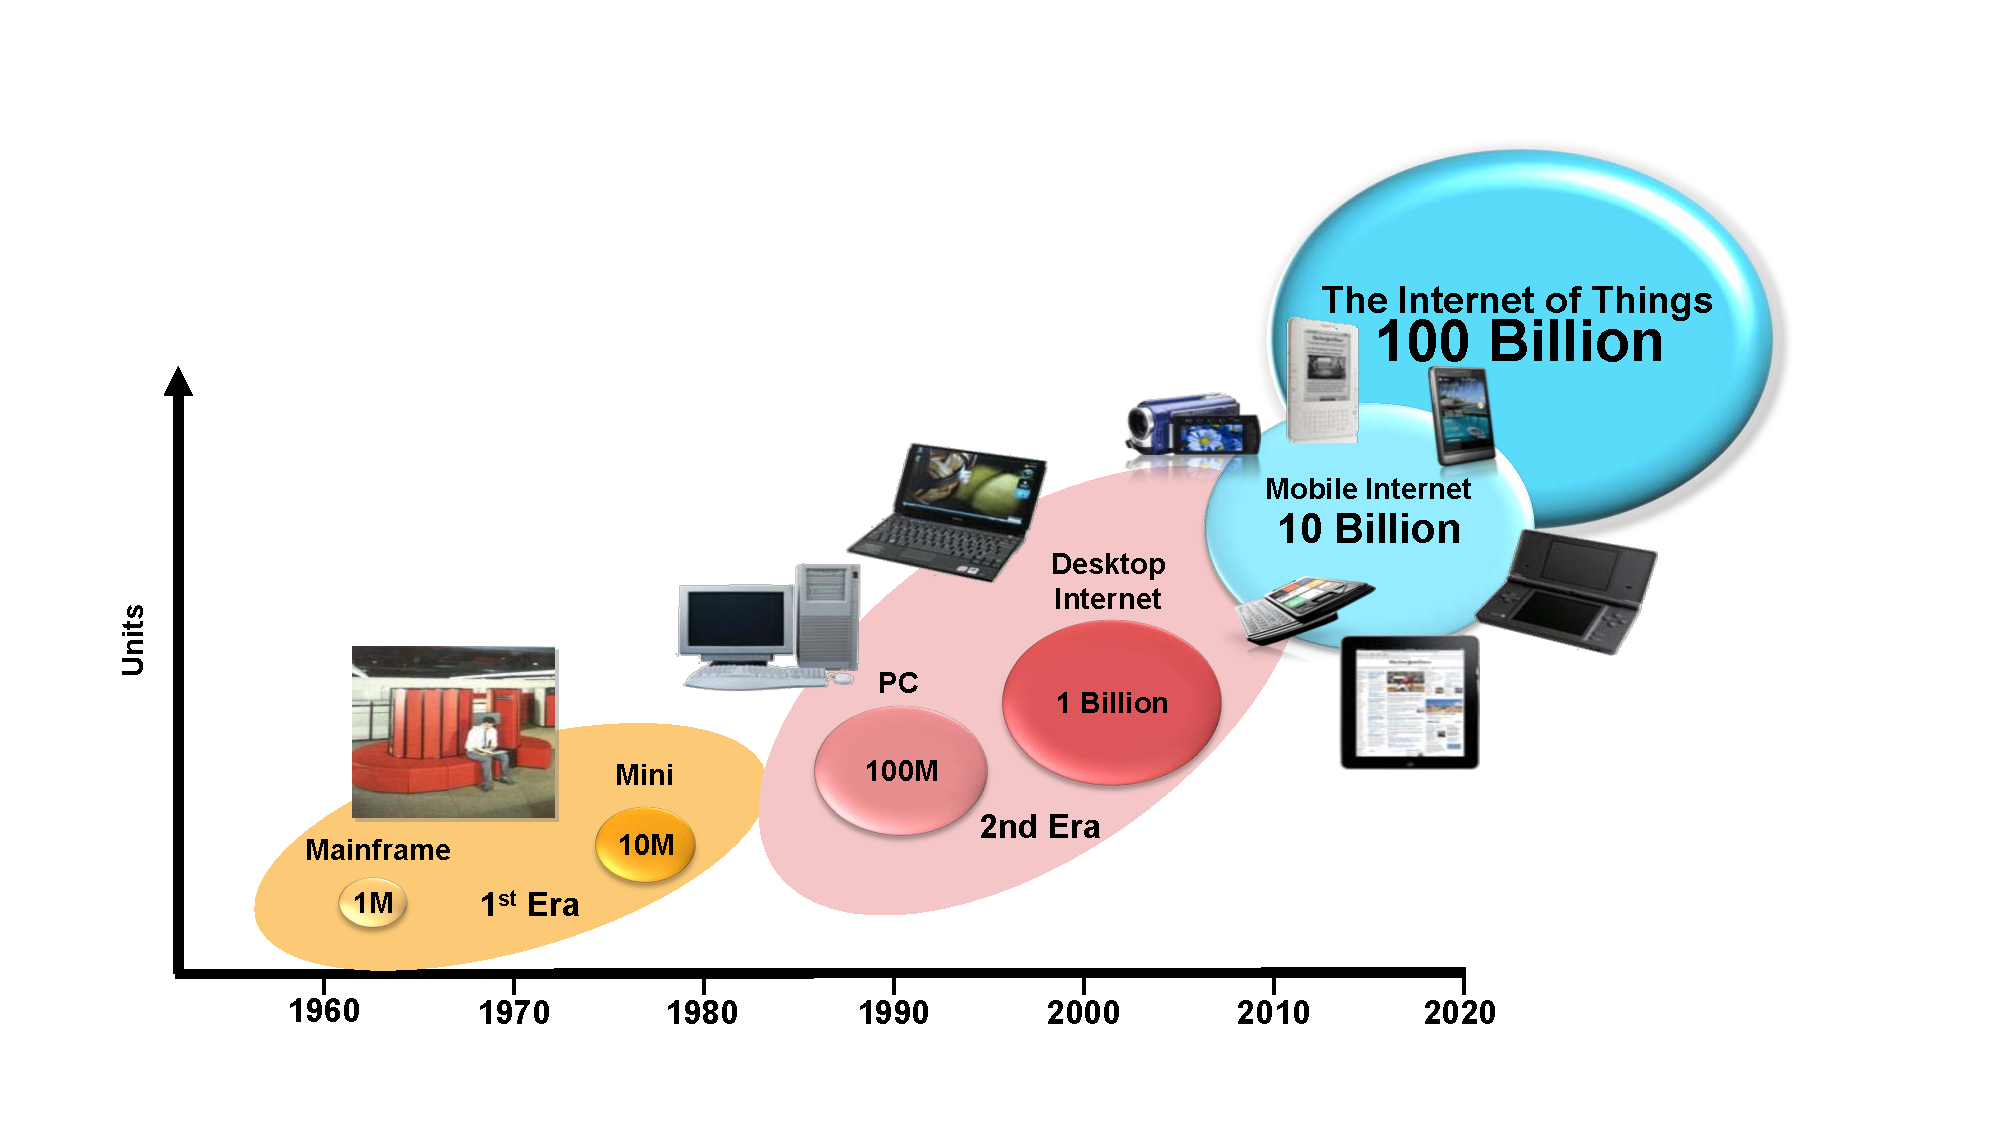
\includegraphics[width=\textwidth]{enc/imagens/CompEras.pdf}
    Fonte:~\textcite{ARM2013}
\end{figure}


As bases teóricas e princípios da Engenharia de Computação remetem a computação, matemática, ciência e engenharia resolvendo problemas técnicos por meio do \textit{design} de dispositivos computacionais, \textit{software}, redes e processos \cite{CE2016}. Essas bases teóricas sustentam a atuação profissional em diferentes áreas, como melhor descrito na Seção~\ref{sec:atuacao}.


\section{Campos de Atuação Profissional}~\label{sec:atuacao}

\textcolor{red} {O Anexo II da Resolução do CONFEA n° 1010, de 22 de agosto de 2005, intitulado como Sistematização dos Campos de Atuação Profissional, estabelece as atribuições profissionais do bacharel em Engenharia de Computação no Brasil. Os itens citados na Resolução são:}
\begin{itemize}
    \item Informação: Sistemas, Métodos e Processos da Informação e da Computação.
    \item Sistemas Operacionais: Organização de Computadores. Compiladores.
    Paradigma de Programação. Algoritmos e Estrutura de Dados. Softwares Aplicados à Tecnologia.
    \item Pesquisa Operacional: Modelagem, Análise e Simulação de Sistemas. Expressão Gráfica Computacional.
    \item \textit{Hardware}: Redes Lógicas. Técnicas Digitais. Informática Industrial.
    Instalações, Equipamentos, Componentes e Dispositivos de Mecânica Fina, Elétricos, Eletrônicos, Magnéticos e Ópticos da Engenharia de Computação.
\end{itemize}


\section{Objetivos do Curso}
\label{sec:objetivos}

O objetivo geral do Curso de Engenharia de Computação é a preparação de profissionais para serem capazes de receber e atender demandas e responsabilidades em um campo de atuação amplo que inclui:
\begin{itemize}
    \item Atuação em empresas de tecnologia e \textit{start ups} que desenvolvem sistemas computacionais (hardware e/ou software), tais como: Apple, Samsung, Amazon, Foxconn, Alphabet Inc., Microsoft, Huawei, etc.
    % parece estranho listar essas empresas aqui: por que essas e não outras? e se alguma 'pisar na bola'? vale a pena manter esta lista aqui?  (helio)
    \item A prática da Engenharia de Computação no mercado em diferentes verticais de atuação tais como: Agronegócio, Saúde, Aviação, Energia, Mineração, Petróleo, Finanças, Educação, Varejo, Serviços, Telecomunicações e Governo entre outras;
    \item Carreiras acadêmicas em Engenharia de Computação, através de uma sólida preparação para pós-graduação e posteriormente atuação no ensino, pesquisa e extensão.
\end{itemize}

O profissional formado em Engenharia de Computação (EC) deverá possuir a competência (conhecimento, habilidade e atitude) para atuar em diferentes áreas, incluindo Engenharia Elétrica, Engenharia de Automação, Engenharia de Produção, Tecnologia da Informação, Ciências da Computação e Física, entre outras áreas, de forma que habilita o egresso a ter competências para entender, mapear, propor e implementar soluções integradoras que atendam os requisitos do problema através de execução de projeto de engenharia que atenda a demanda.
% parece estranho indicar que o profissional pode atuar em áreas de formação de outros cursos. (helio)

Essas competências são adquiridas por meio de núcleos de formação que contemplam aspectos técnicos e também humanísticos, componentes curriculares que tratam as ações práticas, de saber fazer, conjuntamente com os aspectos teóricos e corpo docente qualificado e atuante nas esferas do ensino, da pesquisa e da extensão, criando oportunidades de aprendizado em sintonia com as demandas do mercado e da sociedade.


\section{Justificativa da Criação do Curso na UFSCar e sua Evolução Institucional}


O curso de Engenharia de Computação da UFSCar, implantado em 1992, e contemplando trinta vagas, foi aprovado através do Parecer n° 275/92, de 15 de abril de 1992, do Conselho de Ensino e Pesquisa e da Resolução n° 133/92, de 07 de maio de 1992, do Conselho Universitário da Universidade Federal de São Carlos, sendo reconhecido pela Portaria MEC n° 919, de 21 de agosto de 1998, cuja renovação do reconhecimento ocorreu através da Portaria SERES/MEC n° 286, de 21 de dezembro de 2012 (D.O.U. 27/12/2012).

O curso foi criado para atender às necessidades do mercado de trabalho que exigia profissionais com formação plena em engenharia e formação profissional em computação, pautado pelas diretrizes da Resolução CEF n° 48/76.

Nessa perspectiva, o curso almejava formar profissionais que projetassem sistemas computacionais, ou adaptasse os existentes, a partir do levantamento das necessidades de uma organização, dos estudos relativos à viabilidade técnica e custos do projeto, bem como realizaria o acompanhamento de todas as etapas da produção industrial. Esse profissional também seria formado para participar de projetos em indústrias, elaborando e utilizando novas técnicas de programação, modelagem e simulação de sistemas, que garantissem o emprego eficiente dos recursos computacionais.

% A Matriz Curricular de 1992 encontra-se no Anexo~\ref{cha:Matriz1992}, na qual as disciplinas são separadas por semestre e número de créditos. A distribuição da carga horária do curso também pode ser observada no Anexo~\ref{cha:Matriz1992} e a quantidade de créditos e as horas das disciplinas, divididas em seus tipos de Formação e referentes à Legislação Específica também.

Em 1996, ainda durante o processo de implantação do Curso de Bacharelado em Engenharia de Computação foi realizada a primeira autoavaliação com a participação de 4 (quatro) turmas de discentes, docentes e técnico-administrativos. Esse processo de autoavaliação vinculou-se ao Programa de Avaliação Institucional das Universidades Brasileiras (PAIUB), com financiamento da Secretaria de Ensino Superior (SESu/MEC), tendo o curso sido analisado considerando o perfil do profissional formado, os currículos e programas, as condições de funcionamento e os desempenhos docente e discente. Um resumo dos principais resultados da autoavaliação do PAIUB encontra-se em~\textcite{CPA}.

Em 1998, foi realizada a avaliação externa no período de reconhecimento do Curso pela equipe de avaliadores externos e nomeados pelo Ministério da Educação e Cultura (MEC). Os resultados dessa avaliação externa foram considerados positivos e um resumo dos indicadores da avaliação podem ser encontrados em~\textcite{CPA}. Nessa ocasião, a partir dos dados relativos à autoavaliação e avaliação externa, a carga horária total foi alterada de 252 (3.780 horas) para 250 créditos (3.750 horas), bem como algumas alterações na matriz curricular foram implementadas.

%De modo geral, essas alterações foram pautadas pelas mudanças identificadas no mercado de trabalho, ou seja, se fazia necessário propiciar o desenvolvimento de competências para a resolução de problemas que surgiram com o processo de implantação da Internet no Brasil. %A nova matriz elaborada em 1999 encontra-se no Anexo~\ref{cha:Matriz1999}.

A primeira reformulação curricular foi implementada em 2006 e pautou-se pela ampliação de conteúdos do núcleo básico, reorganização das práticas de laboratório para subsidiar a solução de problemas baseados na integração dos projetos multidisciplinares então existentes. A inclusão de disciplinas optativas vinculadas às linhas de pesquisa do corpo docente do Departamento de Computação seja no Programa de Mestrado em Ciência da Computação, como no Programa de Mestrado em Biotecnologia propiciou uma formação geral sólida para que o discente pudesse: (i) atuar nos mais diversos ramos de atividades da Engenharia de Computação; (ii) buscar consolidar a realização de seus interesses individuais; e (iii) estivesse preparado para enfrentar os desafios tecnológicos. Outro aspecto da avaliação vinculado à reformulação se refere ao Exame Nacional de Desempenho de Estudantes (ENADE) para os cursos de Computação, realizado pela primeira vez em 2005, quando entre estudantes com as melhores notas, figuraram os do curso de Bacharelado em Engenharia de Computação da UFSCar, campus São Carlos.

Em 2015 foi instituída uma comissão para a reformulação do projeto pedagógico, motivada pelos avanços tecnológicos, novos aspectos sócios econômicos existentes e novas avaliações do curso realizadas pela Comissão Própria de Avaliação (CPA) da UFSCar, criada a partir da publicação da Lei n° 10.861 de 14 de abril de 2004, que instituiu o Sistema Nacional de Avaliação da Educação Superior (SINAES). Este projeto pedagógico foi aprovado em 2018 (aprovado pelo Conselho de Curso da EC em sua 45ª reunião ordinária de 12/07/2018 e pelo Conselho do Departamento de Computação em sua 3ª reunião extraordinária de 13/07/2018) e implementado para os ingressos de 2019, de forma que a primeira turma concluirá o curso no final de 2023. As alterações no curso se caracterizaram por um melhor balanceamento da carga horária das disciplinas, com ênfase maior em disciplinas de \textit{hardware}. De forma geral, o curso como um todo teve sua carga horária total reduzida para 3.660~horas e teve como alterações relevantes a inserção de disciplinas eletivas e o cumprimento obrigatório de atividades complementares, com destaque a projetos integradores com caráter extensionista. Tais modificações permitiram que o curso assumisse uma identidade própria, tanto frente a outros cursos de Engenharia de Computação quanto aos demais cursos a área de Computação. 

% TODO: pensar se deixa simples ou mais completo o texto...
%Em 2019 foram instituídas as novas Diretrizes Curriculares Nacionais de Ensino (DCNs), as quais trazem, entre outros aspectos, a ênfase no desenvolvimento de competências técnicas e sócio emocionais dos estudantes ao longo da sua trajetória de formação. 

\textcolor{red}{As Diretrizes Curriculares Nacionais (DCNs) para as Engenharias, instituídas pela Câmara de Educação Superior do Conselho Nacional de Educação (CES/CNE) através da Resolução nº 02/2019, definem os princípios, os fundamentos, as condições e as finalidades, para aplicação, em âmbito nacional, na organização, no desenvolvimento e na avaliação do curso de graduação em Engenharia das Instituições de Educação Superior (IES). Elas trazem, entre outros aspectos, a ênfase no desenvolvimento de competências técnicas e sócio emocionais dos estudantes ao longo da sua trajetória de formação, buscando criar um ambiente propício para o desenvolvimento do pensamento criativo, com sólida base teórica, da capacidade de inovação e de empreendedorismo dos graduandos em engenharia. Neste contexto, o anexo A busca adequar o PPC do curso de Bacharelado em Engenharia de Computação para atender às referidas diretrizes segundo o perfil do profissional a ser formado pela UFSCar (ref?).}  % TODO: Rever este texto frente à incorporação de extensão.

% acho que falta também uma ligação desta informação com o conteúdo desta seção. (helio)


\chapter{Marco Conceitual do Curso}\label{cha:MarcoConceitual}
%%%%%%%%%%%%%%%%%%%%%%%%%%%
% Marco Conceitual do Curso

O profissional formado em Engenharia de Computação (EC) deverá possuir a competência (conhecimento, habilidade e atitude) para atuar em diferentes áreas, incluindo Engenharia Elétrica, Engenharia de Automação, Engenharia de Produção, Tecnologia da Informação, Ciências da Computação e Física, entre outras áreas agregadas ao curso de Engenharia de Computação. Desta forma, habilita o egresso ter capacidade de entender, mapear, propor e implementar soluções integradoras que atendam os requisitos do problema através de execução de projeto de engenharia que atenda à demanda.

% "deverá possuir a competência" ? Será que é melhor dizer que "terá a competência para..." ? (helio)
% ^^^-----------Concordo (jander)

% Será que é certo dizer que o EC pode atuar em EE, EA, EP, TI, CC, F, etc.? Será que não é preciso mencionar "em áreas releacionadas a essas formações?  (helio)

\textcolor{red}{No ano de 2000, em um trabalho conjunto elaborado por coordenadores e 
representantes das Comissões de reformulaçao
 Curricular dos Cursos de Graduação e a
Pró-Reitoria de Graduação da UFSCar, foi estabelecido o perfil do profissional a ser formado pelos cursos de graduação estabelecendo-se as competências necessárias a serem adquiridas pelo egresso, documento este que foi revisado em 2008 (UFSCar, 2008). Este documento estabelece as competências gerais a serem adquiridas durante a graduação da UFSCar. Sendo estabelecidos um conjunto de oito competências gerais, descritas a seguir:}
\textcolor{red}{\begin{itemize}
    \item Aprender;
    \item Produzir;
    \item Empreender;
    \item Atuar;
    \item Comprometer;
    \item Gerenciar;
    \item Pautar;
    \item Buscar
\end{itemize}}

\textcolor{red}{Neste documento, do Perfil do Profissional a ser Formado na UFSCar (UFSCar, 2008), também formam definidas as competências específicas do profissional a ser formado, isto é, estabelece o detalhamento das competências gerais, de acordo um uma interpretação geral para todos os cursos de graduação da UFSCar.}

\textcolor{red}{A partir das competências gerais e das competências específicas estabelecidas, o NDE do curso de EC, realizou a revisão das competências específicas, adaptando-o para o curso de Bacharelado em Engenharia de Computação.}

%Assim foi estabelecida uma nova leitura das competências específicas, agora aptadas para o curso de EC, como descrito no anexo A deste PPC.

% Desta forma, o curso se caracteriza pela agregação de conhecimento de diferentes áreas, particularmente de Engenharia Elétrica e Ciências da Computação, o que confere ao profissional a capacidade de analisar, especificar, projetar, implementar, integrar, testar e manter sistemas computacionais completos, modulares, autônomos, integrados, móveis, distribuídos, inteligentes, complexos ou dedicados, baseados em tecnologias de hardware e software que automatizem a execução de processos dos problemas de engenharia de computação.}


\section{Competências Gerais da Formação do Engenheiro de Computação}\label{sec:competencias-gerais-da-formacao-do-engenheiro-de-computacao}

\textcolor{red}{As competências gerais da formação do Engenheiro de Computação deverão tratar dos conhecimentos, das habilidades e da atitude profissional adquiridos pelo egresso durante o curso classificadas de acordo com o Perfil do Profissional a ser Formado na UFSCar (UFSCar, 2018), isto é, Aprender, Produzir, Empreender, Atuar, Comprometer, Gerenciar, Pautar e Buscar. Os conhecimentos devem ser necessários e suficientes para que o egresso possa atuar com segurança e domínio do assunto em todas as atividades relacionadas ao Engenheiro de Computação, enquanto deverá, durante o curso, desenvolver habilidades na busca de soluções de problemas. Deverá também possuir uma compreensão adequada do mundo e da sociedade, levando em consideração aspectos humanísticos, estando capacitado a atuar de forma proativa, ética e profissional para solucionar os problemas relacionados.}
% "... deverão tratar..." ?  ou "tratam, estão relacionadas, ...?  (helio)
\textcolor{red}{Para tal, poderá fazer uso de diferentes tecnologias e estratégias, propondo soluções criativas e inovadoras para a sociedade, implementadas como sistemas computacionais e contribuindo diretamente para o desenvolvimento sustentável do país e para a geração de riqueza, dentro dos princípios da ética profissional.}
% Para tal, o egresso do curso poderá fazer uso... (?) (helio)

O egresso possuirá, assim, o conhecimento e as habilidades para atuar em diferentes indústrias, no ensino, na pesquisa e na extensão ou, ainda, empreender novos negócios.

Adicionalmente, o engenheiro de computação estará capacitado a entender e considerar aspectos de negócios no processo de desenvolvimento, como o gerenciamento de projetos de engenharia de computação, e possuirá a habilidade de adaptação à constante e rápida evolução da área, aprendendo de forma autônoma e contínua. Também estará apto à produção e à divulgação de novos conhecimentos, tecnologias, serviços e produtos.


\section{Competências Específicas da Formação do Engenheiro de Computação}\label{sec:competencias-especificas-da-formacao-do-engenheiro-de-computacao}

O curso de Engenharia de Computação deverá proporcionar ao estudante a capacidade analítica para o entendimento e a resolução de problemas de engenharia de computação, capacidade de interpretação e compreensão de conteúdos de especificações de processos e de tecnologias, e as necessárias competências para o desenvolvimento e condução de projetos. As competências específicas relacionadas a cada uma das competências gerais (UFSCar. 2008) apresentadas irão tratar diretamente da formação do perfil do egresso no mercado de trabalho. Assim, as competências específicas estabelecem o conhecimento, as habilidades e a atitude do egresso para o curso de Bacharelado em Engenharia de Computação e estão distribuídas nas disciplinas oferecidas pelo curso ao longo da graduação do egresso.
% que tal: ".. ao longo da graduação." ? parece estranho falar da graduação do egresso... (h)

\subsection*{Competências específicas para \textsc{Aprender} de forma autônoma e contínua}\label{sec:competencias-especificas-para-aprender-de-forma-autonoma-e-continua}

O curso de Bacharelado em Engenharia de Computação fornecerá ao egresso a competência de aprender relacionada a:

\begin{compitem}
    \item Analisar o problema, processo de execução, entender e aplicar uma metodologia de solução de problemas de engenharia, utilizando técnicas e métodos multidisciplinares da Ciência da Computação e Engenharia Elétrica;
    \item Analisar o desempenho das soluções propostas ou implementadas, através de modelos analíticos, de simulação ou de experimentação;
    \item Analisar documentos de especificação de requisitos para o problema;
    \item Compreender as demandas que devem ser atendidas incluindo os requisitos de usuários, a legislação vigente, as restrições e limites aplicáveis para escolha das tecnologias e soluções;
    \item Compreender especificações técnicas de módulos de software e hardware;
    \item Compreender, analisar e entender normas e padrões documentados para os módulos e tecnologias as serem empregadas na solução;
    \item Aplicar técnicas e restrições para adequação da solução para as normas e padrões técnicos, além das restrições governamentais vigentes no país de uso da solução;
\end{compitem}

\subsection*{Competências específicas para \textsc{Produzir} e divulgar novos conhecimentos, tecnologias e produtos}

Utilizando os conhecimentos e habilidades adquiridas durante o curso de Bacharelado em Engenharia de Computação o egresso será capaz de:

\begin{compitem}
    \item Projetar uma arquitetura de solução prototipada, planejar desenvolvimento de solução definitiva incluindo revisão de módulos de hardware e software e interfaces de integração Inter módulos e com o ambiente destino;
    \item Resolver problemas que demandam conhecimento das tecnologias de automação e controle, para diferentes problemas em diversas áreas e campos de aplicação;
    \item Propor e implementar soluções para problemas que exijam conhecimentos de programação de computadores, conhecimentos matemáticos e físicos dentro dos limites da engenharia;
    \item Propor e implementar soluções que envolvam decisão sobre o design, a estrutura e a arquitetura do software, uso de padrões de projeto, estruturas de desenvolvimento e componentes de software.
    % substituir "design" por projeto? (h)
    \item Propor e implementar soluções para problemas que impliquem no uso de técnicas e programação concorrente, paralelismo, gestão de eventos, comunicação e programação distribuída, controle de execução, manuseio de exceções e erros, sistemas interativos, persistência e coerência de dados;
    \item Propor e implementar soluções para problemas que requeiram o desenvolvimento de software suficientemente complexo para exigir a aplicação de conhecimentos instrumentais às áreas de automação e controle, engenharia de software, e redes de computadores;
    \item Propor, selecionar componentes de hardware e implementar soluções complexas para o sensoriamento e captura de dados com métricas e grandezas, para monitoramento, atuação e controle de ambientes, máquinas, equipamentos, pessoas, objetos e entidades;
    \item Propor, desenvolver e implementar soluções de hardware customizadas para a solução de problemas de engenharia, inclusive com capacidade de reconfiguração flexível através de técnicas baseadas em sistemas em chip;
    \item Produzir, documentar e manter documentação de projeto de forma segura, confiável e aderente à solução implementada, inclusive apontando as restrições legislativas, normativas, éticas e padrões atendidos, com versionamento e identificação de origem;
\end{compitem}

\subsection*{Competências específicas para \textsc{Empreender} formas diversificadas de atuação profissional}

O curso de Bacharelado em Engenharia de Computação fornecerá ao egresso a competência de empreender relacionada a:

\begin{compitem}
    \item Estabelecer novos conhecimentos, tecnologias, serviços e produtos;
    \item Inovar nas soluções de problemas, através da compilação do conhecimento e experiências adquiridas;
    \item Gerar novos negócios em tecnologias nas diferentes áreas do conhecimento; %luciano
    \item Realizar o projeto de produtos e soluções de forma a extrapolar os conhecimentos adquiridos.
\end{compitem}

\subsection*{Competências específicas para \textsc{Atuar} multi, inter e transdiciplinarmente}

No que diz respeito à competência de atuar, o curso de Bacharelado em Engenharia de Computação será capaz de fornecer ao egresso as competências de atuar relacionadas à:

\begin{compitem}
    \item Realização de tarefas práticas em grupo, o que o leva a adquirir a capacidade de liderar e ser liderado;
    \item Habilidade de usar de forma correta a língua portuguesa na forma escrita e falada, através da leitura de materiais bibliográficos, preparação de documentos técnicos, elaboração de relatórios e apresentação de trabalhos de forma oral.
    \item Habilidade de cumprimento de prazos;
    \item Aprendizado e transmissão de conhecimento aos membros da equipe e a conciliação entre teoria e prática;
    \item Capacidade de atuar e trabalhar com equipes multidisciplinares;
    \item Desenvolver e implementar problemas multidisciplinares inovadores relacionados às engenharias e as tecnologias de computação;
    % desenvolver e implementar "soluções para" problemas ... (h)
\end{compitem}

\subsection*{Competências específicas para \textsc{comprometer-se} com a preservação da biodiversidade no ambiente natural e construído, com sustentabilidade e melhoria da qualidade de vida}

O curso de Bacharelado em Engenharia de Computação fornecerá ao egresso a competência de comprometer-se relacionada a:

\begin{compitem}
    \item Entender a necessidade de analisar os impactos de soluções de engenharia em um contexto global, ambiental e social;%luciano
    \item Propor soluções tecnológicas para o desenvolvimento sustentável da sociedade; %luciano
    % será que as soluções propostas levam ao desenvolvimento sustentável, ou que elas devem estar cientes e levar em consideração essas questões? (h)
    \item Propor projetos que estabelecem relações entre o ambiente, as tecnologias e a sociedade;
    \item Propor formas de melhoria da qualidade de vida da sociedade;
\end{compitem}

\subsection*{Competências específicas para \textsc{Gerenciar} processos participativos de organização pública e/ou privada e/ou incluir-se neles.}

No que diz respeito à competência de gerenciar, o egresso do curso de Bacharelado em Engenharia de Computação será capaz de:

\begin{compitem}
    \item Elaborar estratégias para o gerenciamento e controle de desenvolvimento de projetos de sistemas (hardware e software) e soluções em grau de complexidade que demandem o uso e técnicas e modelos de qualidade.
    \item Construir estratégias de desenvolvimento de software e hardware que garantam o funcionamento da solução conforme especificado, através da combinação de técnicas de prototipagem, codificação, validação, testes e homologação dos módulos e conjuntos.
    \item Coordenar a estruturação e execução do projeto de software e hardware para uma plataforma determinada, de forma a atender os requisitos do sistema, documentando as decisões tomadas de forma clara e concisa.
    \item Gerenciar e solucionar problemas que surjam na fase de desenvolvimento de projetos de software e/ou hardware através do uso de estratégias de simulação de interfaces, modelagem de uso em processos de negócio, reutilização de módulos, padronização de interfaceamento e uso de ferramentas e estratégias de gerenciamento do desenvolvimento, com a correspondente documentação de todo o processo.
\end{compitem}

\subsection*{Competências específicas para \textsc{Pautar-se} na ética e na solidariedade enquanto ser humano, cidadão e profissional.}

O curso de Bacharelado em Engenharia de Computação fornecerá ao egresso a competência de pautar-se relacionada a:
% parece estranho dizer "competência de pautar-se...". Será que ficaria melhor algo como "competência para atuar de forma técnica, mas também levando em consideração fatores sociais, como: "   ... ou algo assim.... (h)
\begin{compitem}
    \item Reconhecer, entender e aplicar os limites éticos na solução proposta e ser capaz de descartar soluções que recaiam fora destes limites;
    \item Capacidade de compreender e aceitar as diferenças existentes em uma sociedade na busca de soluções tecnológicas para a melhora da qualidade de vida; % luciano
    \item Analisar os relacionamentos pessoais internos e externos individuais e em grupo;
    \item Reconhecer os limites éticos profissionais e a sua importância na sociedade;
\end{compitem}

\subsection*{Competências específicas para \textsc{buscar} maturidade, sensibilidade e equilíbrio ao agir profissionalmente.}

O curso de Bacharelado em Engenharia de Computação fornecerá ao egresso a competência de buscar relacionada a:
% novamente, talvez seja o caso de não usar "competência de buscar" simplesmente. Talvez, ... a competência de considerar aspectos e conhecimentos de maturidade, respeito e equilíbrio em suas ações relacionadas a:"   ou algo nesse sentido... (h)
\begin{compitem}
    \item Gerenciar ou integrar equipes de trabalho multiculturais, diversas ou plurais;%luciano
    \item Participar como liderança em projetos e na sua participação social;
    \item No desenvolvimento e implantação de projetos relacionados à Engenharia de Computação;
\end{compitem}


\textcolor{red}{Essas competências gerais e especificas, estabelecidas em diálogo com todos os docentes e o NDE do curso de EC, foram sistematizadas de forma a possibilitar um melhor entendimento, ou um entendimento comum entre NDE e os docentes do curso. Assim foi estabelecida uma leitura direcionada às competências específicas, aptadas para o curso de EC de acordo com o Perfil do Profissional a ser Formado na UFSCar (UFSCar, 2008), como descrito no apêndice A deste PPC. O objetivo do apêndice A é o de se estabelecer uma forma mais concisa e objetiva do entendimento das competências e permitir que o NDE possa identificar e avaliar, através dos planos de ensinos formulados pelos docentes de cada disciplina a sua aplicação.}

%%%%%%%%%%%%%%%%%%%%%%%%%%%%%%%%%%%%%%%%%%%%%%%%%%%%%%%%%%%%%%%%%%%%


\section{Estratégias e metodologias de ensino e avaliação}\label{sec:estrategias-e-metodologias-de-ensino-e-avaliacao}

\subsection{Atividades em disciplinas}\label{sec:atividades-em-disciplinas}

% Planilha com estas informações: \url{https://docs.google.com/spreadsheets/d/1bBWnGmKhBWGH3HnDPU2ffqRCjNfU20VQ-vxeyX3qj1A/edit#gid=0}

As atividades listadas abaixo são as possíveis formas de se implementar as competências nas disciplinas do curso de Bacharelado em Engenharia de Computação, sendo que, são aplicadas de forma apropriada de acordo com cada disciplina. Abaixo são apresentas as atividades de acordo com cada competência geral (Anexo~\ref{cha:competencias}).
% essa lista é exaustiva e exclusiva? talvez possa-se dizer "... listadas são exemplos de possíveis ...". 
% também parece estranho falar "formas de implementar as competências...". talvez dizer algo como "formas de avaliar e prover as competências..."   (h)
                         
% achei as listas um pouco redundantes entre si, com itens que aparecem para as diferentes competências... há também características com poucos itens, com bastante desbalanceamento... (h)

\ExecuteLista{\Competencia}{cg-aprender, cg-produzir, cg-empreender,
    cg-atuar, cg-comprometer, cg-gerenciar, cg-pautar, cg-buscar}{
    \subsubsection{\Atributo{\Competencia}{aspecto}}

    \begin{itemize}[noitemsep]
        \ExecuteLista{\Atividade}{\Atributo{\Competencia}{atividades}}{
            \item \Atributo{\Atividade}{descricao}
        }
    \end{itemize}
}


\subsection{Metodologias}\label{sec:metodologias}
Algumas metodologias, ativas ou não, podem ser utilizadas para implementar as competências nas disciplinas, sendo umas mais apropriadas que outras, de acordo com a competência que se deseja transmitir. São elas:

% esta seção está estranha, parece que sem um propósito definido: essas metodologias são usadas no curso? Só listá-las aqui parece não ser muito objetivo (h)

\begin{itemize}
    \item Apresentação de seminários e discussões em grupos;
    \item Metodologia Design Thinking;
    \item Metodologia PBL – Aprendizagem Baseada em Problemas;
    \item Metodologia PjBL - Aprendizagem Baseada em Projetos;
    \item Metodologia TBL - Aprendizado baseado em Times (Grupos);
    \item Metodologias baseada em Estudo de Casos;
    \item Metodologias que possibilitam ao discente maior tempo e profundidade no desenvolvimento de tarefas de laboratório. Poderia ser utilizado o Espaço Maker do DC;
    \item Sala de aula invertida;
    \item Trabalho em grupo.
\end{itemize}

\subsection{Avaliação}\label{sec:avaliacao}

Por outra parte, torna-se necessário proporcionar aos estudantes vários momentos de avaliação, multiplicando as suas oportunidades de aprendizagem e diversificando os métodos utilizados. Assim, permite-se que os estudantes apliquem os conhecimentos que adquirem, exercitem e controlem eles próprios a aprendizagem e o desenvolvimento das competências, recebendo feedback frequente sobre as dificuldades e progressos alcançados.

O Regimento prevê ainda a realização de procedimentos e/ou aplicação de instrumentos de avaliações em, pelo menos, três datas distribuídas no período letivo para cada disciplina/atividade curricular. Serão considerados aprovados os estudantes que obtiverem frequência igual ou superior a setenta e cinco por cento das aulas e desempenho mínimo equivalente à nota final igual ou superior a seis.
% Qual regimento é este? Do que se trata? (h)

% parece estranho falar em "recomendação" neste documento. Afinal, ele é uma apresentação do curso e não um guia para os docentes que forem preparar suas disciplinas, certo? 
% essa estória de nota e fre
A utilização de diferentes métodos e instrumentos de avaliação é recomendada. A escolha dos métodos e instrumentos de avaliação depende de vários fatores: das finalidades, do objeto de avaliação, da área disciplinar e nível de grau de conhecimento dos estudantes a que se aplicam, do tipo de atividade, do contexto, e dos próprios avaliadores. Portanto, propõe-se que, além da tradicional prova individual e trabalho em grupo, outras formas de avaliação das atividades elencadas para se implementar as competências podem ser sugeridas abaixo:

\begin{itemize}
    \item Apresentação de projetos e avaliação em grupo;
    \item Apresentação de relatórios em seminários;
    \item Apresentações, relatórios, exercícios periódicos;
    \item Avaliação por pares;
    \item Compartilhamento das soluções entre grupos distintos;
    \item Emprego de metas (com soluções esperadas) a serem alcançadas;
    \item Identificação de evolução do material trazido e compartilhado, em uma abordagem coletiva e em pares;
    \item Observação e apresentação dos resultados de desenvolvimento prático;
    \item Realização de avaliações formativas e somativas;
    \item Verificação da funcionalidade e o desempenho de programas desenvolvidos;
    \item Verificação se as soluções desenvolvidas atendem às especificações.
\end{itemize}
                                           


\chapter{Marco Estrutural do Curso}~\label{cha:MarcoEstrutural}
%! Author = NDE
%! Date = 27/02/2023

O marco estrutural do Curso de Bacharelado em Engenharia de Computação da UFSCar, campus de São Carlos, engloba os seguintes componentes curriculares: Disciplinas Obrigatórias, Extensionistas e Optativas,  Atividades Complementares, Trabalho de Conclusão de Curso e Estágio Obrigatório. A estrutura visa atender a \citetitle{CNE2019}, a qual estabelece as Diretrizes Curriculares Nacionais (DCNs) para as Engenharias, tendo sido instituída pela Câmara de Educação Superior do Conselho Nacional de Educação (CES/CNE).

% \begin{quote}
%     ``Institui as Diretrizes Curriculares Nacionais para os
%     cursos de graduação na área da Computação,
%     abrangendo os cursos de bacharelado em Ciência
%     da Computação, em Sistemas de Informação, em
%     Engenharia de Computação, em Engenharia de
%     Software e de licenciatura em Computação, e dá
%     outras providências.''
% \end{quote}
% \footnote{A Resolução CNE/CES 11/2002 foi publicada no Diário Oficial da União em 9 de abril de 2002, Seção 1, p.32}.
%\footnote{CNE. Resolução CNE/CES 5/2016. Diário Oficial da União, Brasília, nº 220, de 17 de novembro de 2016 – Seção 1 – págs. 22 á 24}

%%%%%%kelen

% Art. 6º Resolução CNE/CES nº 5, de 16 de novembro de 2016 Os currículos dos cursos de bacharelado e licenciatura da área da Computação deverão incluir conteúdos básicos e tecnológicos referentes à área da Computação, comuns a todos os cursos, bem como conteúdos básicos e tecnológicos específicos para cada curso, todos selecionados em grau de abrangência e de profundidade de forma consistente com o perfil, as competências e as habilidades especificadas para os egressos.
%§ 1º Estes conteúdos não consistem em disciplinas obrigatórias, mas no conjunto substantivo de conhecimentos que poderão ser selecionados pelas Instituições de Educação Superior para compor a formação dos egressos em cada curso em questão.
%§ 2º Os conteúdos poderão ser ministrados em diversas formas de organização, observando-se o interesse do processo da formação acadêmica e a legislação vigente, e deverão ser planejados de modo integrado, dando sentido de unidade ao projeto pedagógico do curso.
%§ 3º Para a licenciatura deverão ser incluídos conteúdos de formação pedagógica, considerando as Diretrizes Curriculares Nacionais para a formação de professores para a Educação Básica.
%§ 4º Os núcleos de conteúdos poderão ser dispostos, em termos de carga horária e de planos de estudo, em atividades práticas e teóricas, individuais ou em equipe, tais como:

Assim, de acordo com a \citetitle{CNE2019}, tendo em consideração a flexibilidade necessária para atender domínios diversificados de aplicação e as vocações institucionais ao perfil do egresso, o Curso de Bacharelado em Engenharia de Computação provê uma formação sólida em Ciência da Computação, Matemática e Eletrônica. Essa formação se dá por meio de conteúdos básicos e tecnológicos referentes à área da computação, bem como conteúdos básicos e tecnológicos específicos para o curso de Engenharia de Computação. Estes conteúdos são abordados em grau de abrangência e de profundidade de forma consistente com o perfil do egresso, visando desenvolver as competências e as habilidades essenciais na formação de um Bacharel em Engenharia de Computação. A representação do perfil de formação é apresentada na Figura~\ref{fig:perfil}.

\textcolor{red}{\Large \textbf{Necessidade de revisão a partir daqui quando tivermos mais material sobre a curricularização da extensão.
Reunião dia 16/02/2024:
Revisar item 4 (daqui em diante)
Alterar Objetivos incluindo competências gerais
Produzir versão 1.0 até 20/Abril/2024
Fazer Revisão geral
}}


\begin{figure}[H] %TODO: vou trocar os 3 núcleos pelas 3 áreas: Computação, Matemática e Eletrônica
    \centering
    \caption{Representação Gráfica do Perfil de Formação}
    \label{fig:perfil}
    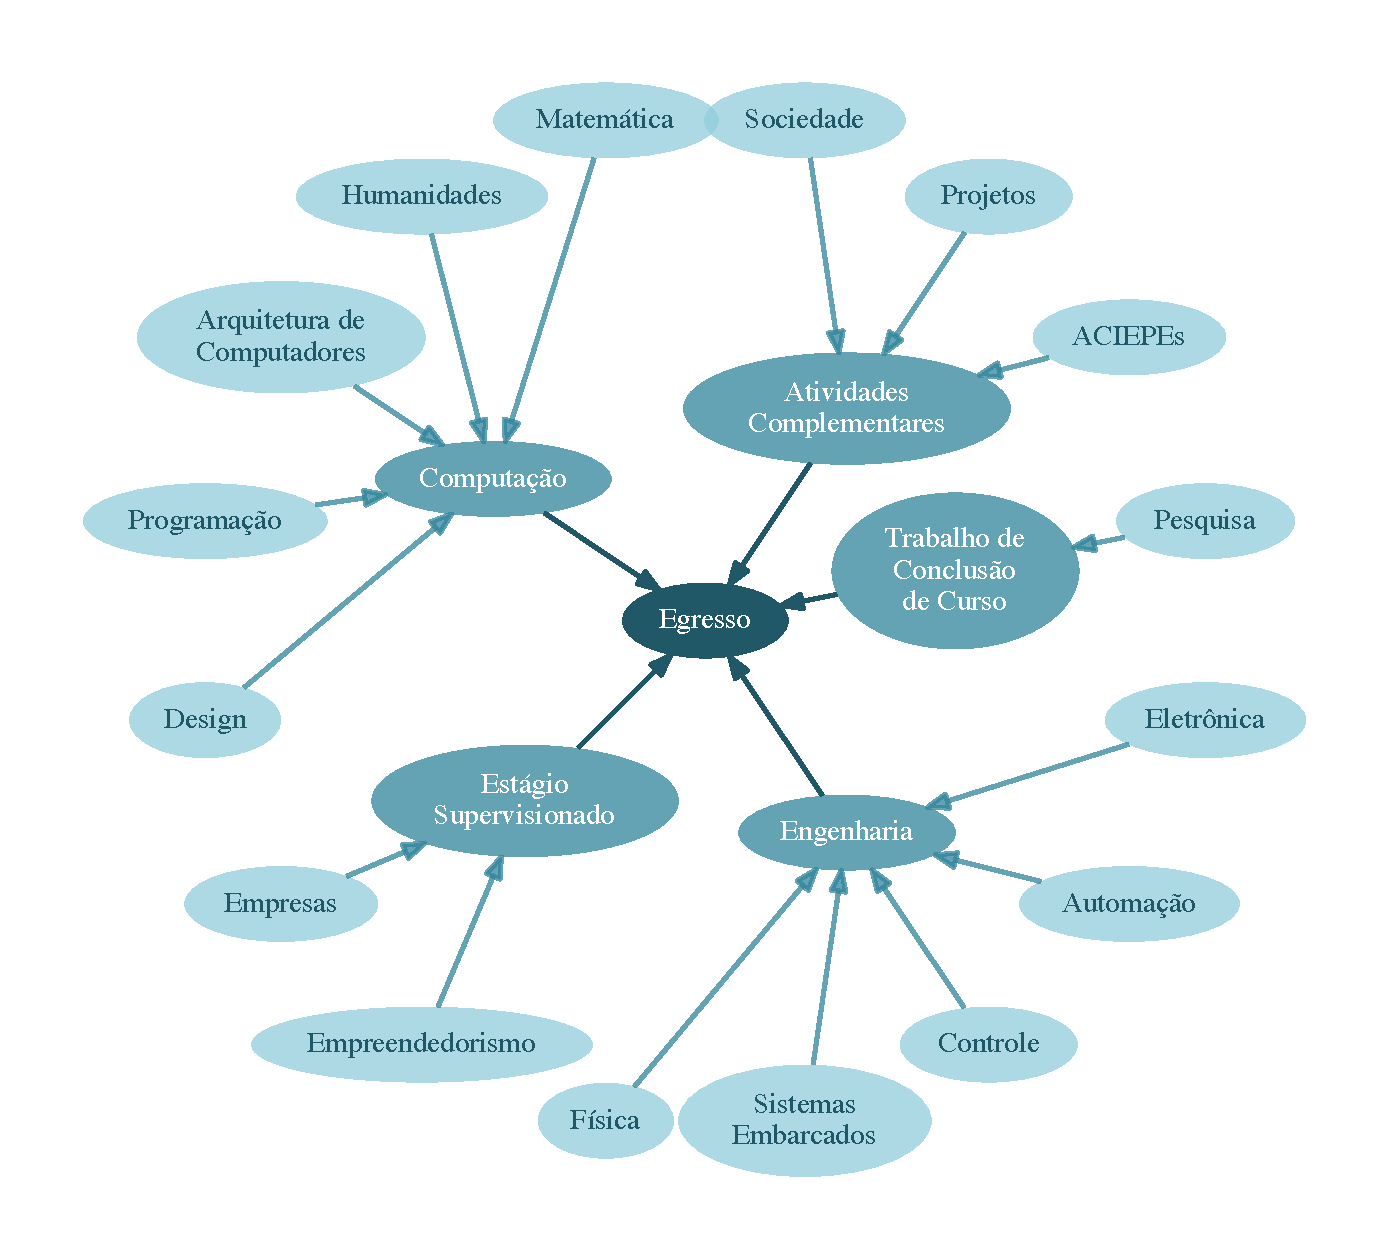
\includegraphics[width=\textwidth]{enc/imagens/Perfil.pdf}
\end{figure}

No Curso de Bacharelado em Engenharia de Computação, os conteúdos são apresentados por eixos que agrupam vários componentes curriculares, cada eixo é detalhado na Seção~\ref{sec:ACMC}. Os conteúdos básicos e tecnológicos referentes à área da computação compõem os eixos: Fundamentos de Matemática e Estatística, Algoritmos e Programação, Arquitetura de Computadores, Metodologias e Técnicas de Computação e Humanas. Estes eixos constituem um grupo de disciplinas de ciências básicas que oferecem uma formação elementar ao estudante referente aos campos de conhecimentos das ciências exatas, das ciências humanas e de computação básica.

Os conteúdos básicos e tecnológicos específicos para o Curso de Bacharelado em Engenharia de Computação consistem nos eixos: Física, Eletrônica, Engenharia e Sistemas e Especialização. Nesses eixos se concentram os conteúdos relacionados à capacitação do estudante ao exercício profissional da Engenheira de Computação. Os conteúdos abordados no eixo de Engenharia e Sistemas se caracterizam pela especificidade em relação às extensões e aprofundamentos profissionalizantes caracterizando o Curso de Bacharelado em Engenharia de Computação e fornecendo ao estudante conhecimentos científicos, tecnológicos e instrumentais próprios da área. O eixo Especialização fornece conhecimento em áreas específicas e também colabora para tornar o curso mais flexível às alterações científicas e tecnológicas, permitindo também ao aluno optar por um curso que se adapte a suas habilidades ou a demandas específicas do mercado.

De acordo com a \citetitle{CNE2019}, no conteúdo curricular se deve assegurar na formação o conhecimento das questões sociais, profissionais, legais, éticas, políticas e humanísticas. Pelo \citetitle[Seção II, Art. 14]{RGCG} e o \citetitle{PDI-UFSCAR}, conforme Parecer ConsUni nº 337 de 08/11/2003, bem como reafirmadas e ampliadas no PDI/UFSCar, conforme a Resolução ConsUni/UFSCar nº 766 de 20/12/2013, e do Perfil do Profissional a ser formado na UFSCar, conforme o Parecer CEPe/UFSCar nº 776 de 30/03/2001, também deve-se assegurar o conhecimento das temáticas relacionadas à História e Cultura Afro-Brasileira e Indígena, Língua Brasileira de Sinais (LIBRAS), Educação em Direitos Humanos e Educação Ambiental.
Esses conteúdos serão trabalhados de forma transversal nas disciplinas Seminários 1 e Seminários 2, bem como em Disciplinas Eletivas e Atividades Complementares que os estudantes devem desempenhar. %TODO: bem como em Disciplinas Eletivas e Atividades Complementares que os estudantes devem desempenhar ( o que acham?)
% sendo incorporados nas temáticas ambiental, diversidade cultural, desigualdades sociais, cidadania, empreendedorismo, administrativas, étnico-racial e cultural, sustentabilidade e impacto da computação e suas tecnologias na sociedade.

As Atividades Complementares são atividades curriculares que não estão compreendidas no desenvolvimento regular das disciplinas do Curso, compreendendo
% https://www.overleaf.com/download/project/5afb872df2e25c77af324668/build/17948239805-f5d853681d1bc600/output/output.pdf?compileGroup=standard&clsiserverid=clsi-pre-emp-e2-b-zrw3&popupDownload=true
outras atividades de caráter acadêmico, científico, social e cultural realizadas pelo estudante ao longo de seu curso de graduação, e que contribuem para o enriquecimento de conhecimentos de valores e hábitos científicos, profissionais e éticos, como também a colaboração e o trabalho em equipe. As exigências para a realização destas atividades estão relacionadas no Anexo~\ref{cha:atividades_complementares}.

O Trabalho de Conclusão de Curso~(TCC) é um componente curricular obrigatório e constitui-se de um trabalho acadêmico como síntese, integração ou aplicação de conhecimentos adquiridos de caráter científico ou tecnológico relacionado ao curso de Bacharelado em Engenharia da Computação. O TCC será desenvolvido sob a supervisão de um docente vinculado ao Curso de Bacharelado em Engenharia de Computação e formalizado como uma monografia. O objetivo é reforçar os princípios de investigação científica expondo ao estudante temas que incentivem a realização de projetos inovadores e que extrapolem os limites dos conteúdos transmitidos durante o curso. No Anexo~\ref{cha:tcc} é apresentado o Regulamento do Trabalho de Conclusão de Curso com as condições para realização desta atividade.

O Estágio é uma atividade curricular obrigatória realizada no final do curso visando preparar o estudante para o exercício profissional. O Estágio Obrigatório é orientado por um docente do curso por meio de relatórios técnicos e acompanhamento individualizado durante o período de realização do mesmo. O Regulamento do Estágio Curricular Obrigatório e Não-obrigatório pode ser consultado no Anexo~\ref{cha:estagio}.
%%%%%end kelen

%  \begin{comment}
%  De acordo com o Art. 6º da Resolução CNE/CES 11/2002, todo curso de Engenharia, deve possuir em seu currículo um núcleo de conteúdos básicos, um núcleo de conteúdos profissionalizantes e um núcleo de conteúdos específicos que caracterizem a modalidade do respectivo curso. Desta forma, nesse curso de Engenharia da Computação será adotada esta divisão para as componentes curriculares. Na Seção~\ref{sec:ACMC} será apresentado a composição dos núcleos.

% Para o curso de Engenharia de Computação, o  núcleo  de  conteúdos  básicos é constituído por um grupo de disciplinas de ciências básicas e ciências humanas e oferece uma formação elementar ao estudante referente aos campos de conhecimentos da Engenharia. %A carga horária mínima para o núcleo de conteúdos básicos é de 30\% do total previsto.

% No núcleo de conteúdos profissionalizantes, % deve ser composto por cerca de 15\% de carga horária mínima. Neste núcleo
% se concentram os conteúdos relacionados ao exercício profissional do Engenheiro de Computação. Os conteúdos oferecidos nesse grupo iniciarão a capacitação do estudante quando este aplicar os conceitos adquiridos ao conteúdos específicos profissionalizantes do curso de Engenharia de Computação.

% No núcleo de conteúdos específicos, segundo o parágrafo 4º, Art. 6º, da Resolução CNE/CES nº 11/2002, os conteúdos abordados nos módulos se caracterizam pela especificidade em relação às extensões e aprofundamentos do  núcleo  de  conteúdos  profissionalizantes. Desta forma, os conteúdos concentrados nesse núcleo definem o curso de Engenharia da Computação e fornecem ao estudante conhecimentos científicos, tecnólogicos e instrumentais, próprios da área.

% Estes conteúdos serão compostos pelas disciplinas Obrigatórias, Optativas e Eletivas. Todas as disciplinas Obrigatórias foram selecionadas para compor cada núcleo em grau de abrangência e de profundidade de forma consistente com o perfil do egresso, visando desenvolver as competências e as habilidades essenciais na formação de um bacharel em Engenharia de Computação.

% As disciplinas Optativas e Eletivas fornecem aprofundamento em determinadas áreas específicas e também colaboram para tornar o curso mais flexível às alterações científicas e tecnológicas, permitindo também ao estudante, optar por um curso que se adapte a suas habilidades ou a demandas específicas de mercado. A representação do perfil de formação é apresentada na Figura~\ref{fig:perfil}.

% \begin{figure}[H] %TODO: vou trocar os 3 núcleos pelas 3 áreas: Computação, Matemática e Eletrônica
%     \centering
%     \caption{Representação Gráfica do Perfil de Formação}
%     \label{fig:perfil}
%     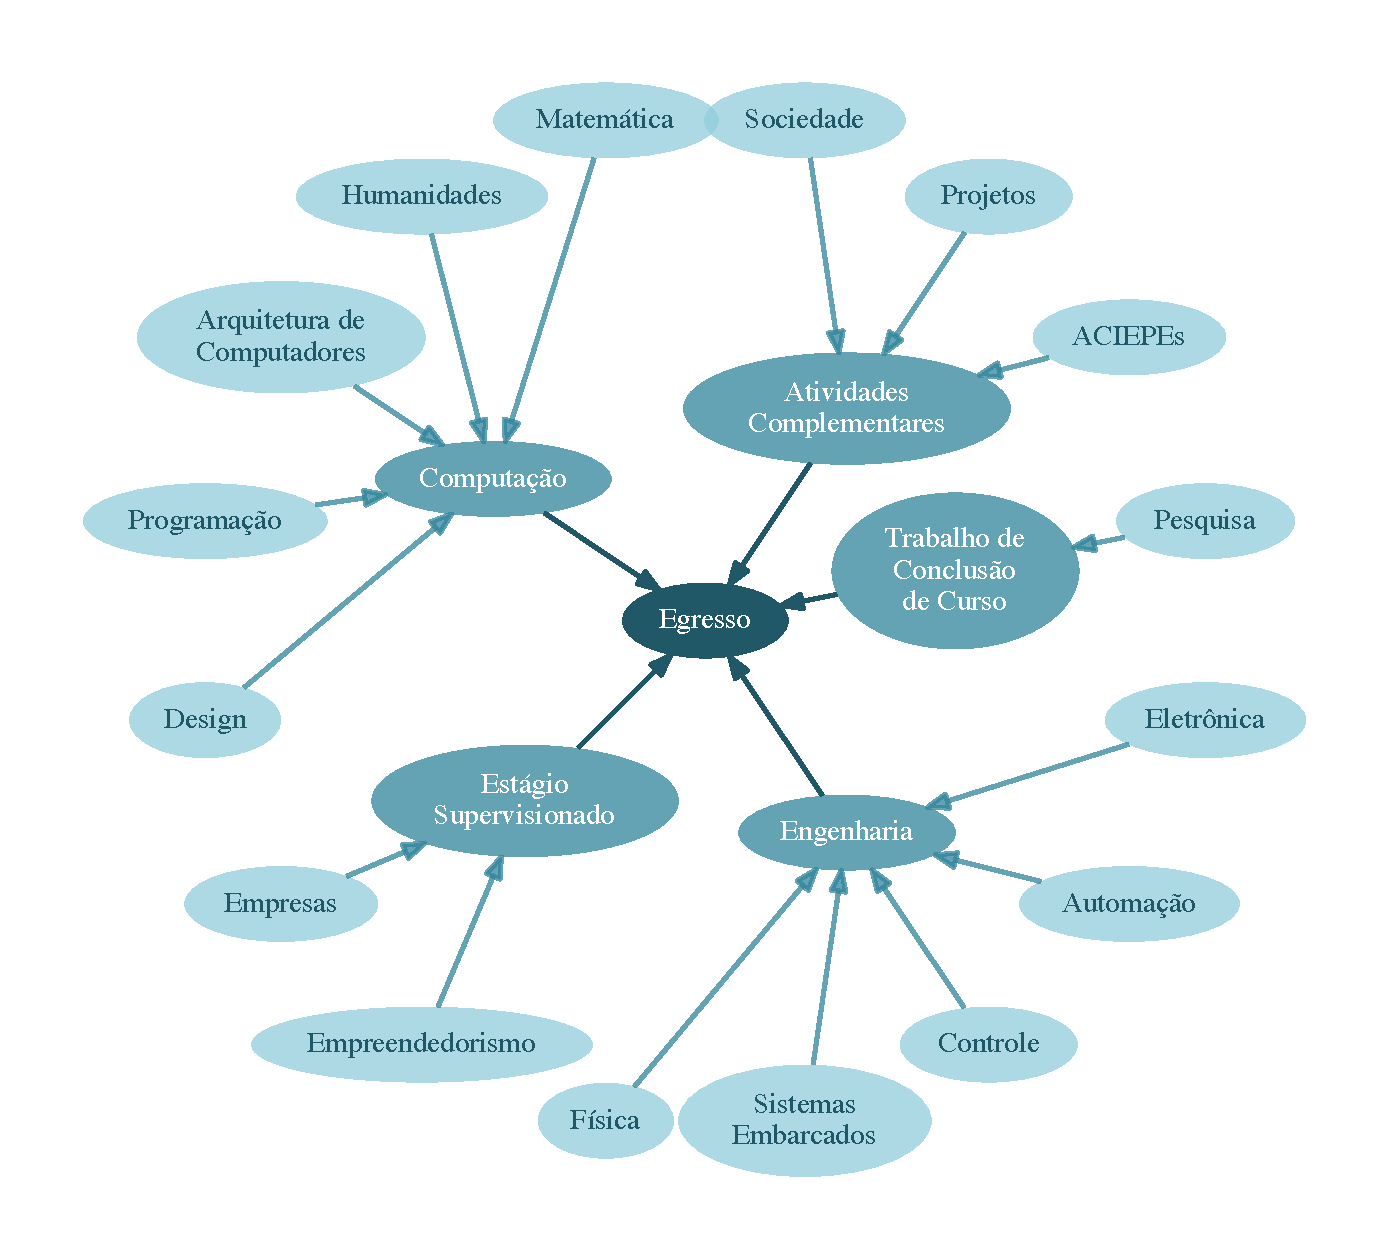
\includegraphics[width=\textwidth]{enc/imagens/Perfil.pdf}
% \end{figure}

% De acordo com o Art. 3º da Resolução CNE/CES 11/2002, no conteúdo curricular deve-se assegurar na formação o conhecimento das questões sociais, profissionais, legais, éticas, políticas e humanísticas. E pelo Regimento Geral dos Cursos de Graduação, Set. 2016 UFSCar (Seção II, Art. 14º)~\cite{RGCG} e o Plano de Desenvolvimento (PDI) da UFSCar~\cite{PDI-UFSCar}, conforme Parecer ConsUni nº 337 de 08/11/2003, bem como reafirmadas e ampliadas; no PDI/UFSCar~\cite{PDI-UFSCar}, conforme a Resolução ConsUni/UFSCar nº 766 de 20/12/2013; e do Perfil do Profissional a ser formado na UFSCar, conforme o Parecer CEPe/UFSCar nº 776 de 30/03/2001; também deve-se asseguar o conhecimento das temáticas relacionadas à História e Cultura Afro-Brasileira e Indígena, Língua Brasileira de Sinais (LIBRAS), Educação em Direitos Humanos e Educação Ambiental.
% Esses conteúdos serão trabalhados de forma transversal nas disciplinas Seminários 1 e Seminários 2, bem como em Disciplinas Eletivas que os estudantes podem vir a cursar.
% % sendo incorporados nas temáticas ambiental, diversidade cultural, desigualdades sociais, cidadania, empreendedorismo, administrativas, étnico-racial e cultural, sustentabilidade e impacto da computação e suas tecnologias na sociedade.

% As Atividades Complementares são atividades curriculares que não estão compreendidas no desenvolvimento regular das disciplinas do Curso, sendo todas e quaisquer atividades de caráter acadêmico, científico, social e cultural realizadas pelo estudante ao longo de seu curso de graduação, e que contribuem para o enriquecimento de conhecimentos de valores e hábitos científicos, profissionais e éticos, como também a colaboração e o trabalho em equipe. As exigências para a realiação destas atividades estão relacionadas no Anexo~\ref{cha:atividades_complementares}.

% %O Projeto Integrador é um componente curricular interdisciplinar que configura-se como eixo articulador para vincular a aprendizagem adquirida ao longo do curso com o aprimoramento de suas habilidades e competências para resolução de problemas contribuindo para o desenvovilmento de sua área.

% %disciplinas de várias eixos de conhecimento visando o desenvolvimento de habilidades e competências que extrapolam o conhecimento adquirido individualmente em cada disciplina.

% % Art. 8º -Resolução CNE/CES nº 5, de 16 de novembro de 2016   O Trabalho de Curso será desenvolvido como atividade de síntese, integração ou aplicação de conhecimentos adquiridos de caráter científico ou tecnológico. Parágrafo único. As Instituições de Educação Superior deverão estabelecer a obrigatoriedade ou não do Trabalho de Curso e aprovar a sua regulamentação, especificando critérios, procedimentos e mecanismo de avaliação, além das diretrizes e técnicas relacionadasà sua elaboração

% O TCC é um componente curricular obrigatório, que de acordo com Art. 7º ~-~Parágrafo Único da CNE/CES 11, 11/2002, constitui-se de um trabalho acadêmico com síntese, integração ou aplicação de conhecimentos adquiridos de caráter científico ou tecnológico relacionado ao curso de Bacharelado em Engenharia da Computação. O TCC será desenvolvido sob a supervisão de um docente vinculado ao curso de Engenharia da Computação e formalizado como uma monografia. O objetivo é reforçar os princípios de investigação cientíca expondo ao estudante temas que incentivem a realização de projetos inovadores e que extrapolem os limites dos conteúdos transmitidos durante o curso. No Anexo~\ref{cha:tcc} é apresentado o Regulamento do Trabalho de Conclusão de Curso com as condições para realização desta atividade.

% O Estágio Supervisionado é uma atividade curricular obrigatória, de acordo com Art. 7º da Resolução CNE/CES 11, 11/2002, realizada no final do curso visando preparar o estudante para o exercício profissional. O Estágio é orientado diretamente por um docente do curso através de relatórios técnicos e acompanhamento individualizado durante o período de realização do mesmo. O Regulamento do Estágio Curricular Obrigatório e Não-obrigatório pode ser consultado no Anexo~\ref{cha:estagio}, com mais detalhes sobre a realização destas atividades.

% \end{comment}

% CNE/CES No:136/2012 Conteúdos Curriculares da Formação Tecnológica e Básica para todos os Cursos de Bacharelado e de Licenciatura
%Os conteúdos tecnológicos e básicos comuns a todos os cursos são: sistemas operacionais; compiladores; engenharia de \textit{software}; interação humano-computador; redes de computadores; sistemas de tempo real; inteligência artificial e computacional; processamento de imagens; computação gráfica; banco de dados; dependabilidade; segurança; multimídia; sistemas embarcados; processamento paralelo; processamento distribuído; robótica; realidade virtual; automação; novos paradigmas de computação; matemática discreta; estruturas algébricas; matemática do contínuo [cálculo, álgebra linear, equações diferenciais, geometria analítica; matemática aplicada (séries, transformadas), cálculo numérico]; teoria dos grafos; análise combinatória; probabilidade e estatística; pesquisa operacional e otimização; teoria da computação; lógica; algoritmos e complexidade; linguagens formais e autômatos; abstração e estruturas de dados; fundamentos de linguagens (sintaxe, semântica e modelos); programação; modelagem computacional; métodos formais; análise, especificação, verificação e testes de sistemas; circuitos digitais; arquitetura e organização de computadores; avaliação de desempenho; ética e legislação; empreendedorismo; computação e sociedade; filosofia; metodologia cientifica; meio ambiente; fundamentos de administração; fundamentos de economia.
% CNE/CES No:136/2012 Conteúdos Curriculares da Formação Tecnológica e Básica dos Cursos de Bacharelado em Engenharia de Computação Os conteúdos básicos e tecnológicos, específicos para os cursos de Engenharia de Computação, são os seguintes: projeto de sistemas digitais; projeto de circuitos integrados; microeletrônica e nanoeletrônica; processamento digital de sinais; comunicação de dados; sistemas de controle; automação de projeto; transdutores; teoria dos semicondutores; teoria eletromagnética; eletrônica digital; eletrônica analógica; circuitos elétricos; eletricidade; física.

O Quadro de Integralização Curricular, contendo a quantidade mínima de créditos exigidos para cada tipo de atividade curricular, é apresentado no Quadro~\ref{tab:integralizacao}.

\begin{table}[H]
    \centering
    \caption{Integralização Curricular}
    \label{tab:integralizacao}
    \begin{tabular}{lcc}
        \sline
        \textbf{Atividades Curriculares} & \textbf{Créditos} & \textbf{Carga Horária} \\
        \hline
        Disciplinas Obrigatórias         & 200               & 3.000                  \\
        Disciplinas Optativas            & 12                & 180                    \\
        Disciplinas Eletivas             & 8                 & 120                    \\
        Estágio Supervisionado           & 12                & 180                    \\
        Trabalho de Conclusão de Curso   & 8                 & 120                    \\
        Atividades Complementares & 4 & 60
        \\
        \hline
        \textbf{Total}                   & \textbf{244}      & \textbf{3.660}         \\
        \sline
    \end{tabular}
\end{table}


\section{Princípios Norteadores da Reformulação Curricular}

Além das motivações já mencionadas na Seção~\ref{sec:objetivos}, a elaboração deste projeto pedagógico foi norteada também por relatos de professores e estudantes do curso e por pesquisa em projetos pedagógicos de cursos de Engenharia de Computação do Brasil e do exterior. Os princípios adotados para a elaboração da matriz curricular deste projeto pedagógico são os seguintes:

\begin{itemize}
    \item \textbf{Caracterização da área de Engenharia de Computação:} Este princípio é contemplado por meio dos núcleos de conteúdos básico e profissionalizantes, que fornecem ao estudante a base teórica necessária para seu engajamento futuro em atividades profissionais na área.
    \item \textbf{Especialização por meio de Disciplinas Optativas:} Este princípio é contemplado por meio de um conjunto de disciplinas Optativas, que cobrem conteúdos avançados, para complementar a formação básica do estudante.
    \item \textbf{Limitação da quantidade de disciplinas por semestre:} Para facilitar a concentração do estudante e permitir que ele tenha uma menor diversidade de conteúdos para gerenciar, a matriz curricular foi projetada para que o estudante curse no máximo 28 créditos por semestre. No entanto, caso o estudante queira se inscrever em disciplinas que não sejam do seu perfil a carga horária máxima semestral está limitada a 32 créditos.
    \item \textbf{Agregação de conteúdos relacionados em uma mesma disciplina:} Buscou-se agregar conteúdos relacionados em uma mesma disciplina, em detrimento de disciplinas distintas, sucessivas ou concorrentes. Por exemplo, a matriz não possui disciplinas distintas para tratar teoria e prática de um mesmo assunto.
    \item \textbf{Aperfeiçoamento de competências de desenvolvimento de projetos:} Este princípio é contemplado por meio de disciplinas presentes no núcleo de conteúdos específicos.
    \item \textbf{Substituição de carga horária teórica por prática:} Em diversas disciplinas buscou-se uma substituição de horas-aula teóricas por atividades práticas e/ou desenvolvimento de projetos.
    \item \textbf{Aprendizado contínuo:} Buscou-se oferecer uma base sólida de conhecimentos e práticas de estudo que permitam ao estudante atualizar-se e aprimorar-se ao longo de toda sua carreira profissional.
    \item \textbf{Consciência do papel do egresso na sociedade:} As disciplinas de Seminários 1 e 2, as disciplinas Eletivas e as Atividades Complementares foram inseridas na matriz curricular para favorecer reflexões sobre o papel do egresso na sociedade.
\end{itemize}


\section{Atividades Curriculares e Matriz Curricular}~\label{sec:ACMC}

% \begin{comment}
% Conforme mencionado, os componentes curriculares foram divididos em núcleo de conteúdos básicos, núcleo de conteúdo profissionalizante e núcleo de conteúdo específicos para o curso de Engenharia de Computação.
% De acordo com o Art. 6º da Resolução CNE/CES 11/2002, o curso deve possuir a proporção da carga horária apresentada a seguir, bem como, apresentar o subconjunto coerente de tópicos para cada núcleo caracterizando a modalidade do curso.

% \begin{compenum}
%     \item A carga horária mínima de 30\% do total previsto para o núcleo de conteúdos básicos;
%     \item Para o núcleo de conteúdos profissionalizantes a carga horária mínima deve ser de 15\%;
%     \item Os conteúdos específicos consubstanciarão o restante da carga horária total;
%     \item A carga horária mínima do estágio curricular deverá atingir 160 (cento e sessenta) horas.
%     \item Deverão também ser estimuladas atividades complementares, tais como trabalhos de iniciação científica, projetos multidisciplinares, visitas teóricas, trabalhos em equipe, desenvolvimento de protótipos, monitorias, participação em empresas juniores e outras atividades empreendedoras.
% \end{compenum}

% Para este curso temos a carga total de 3.900 horas de atividades, estando divididas conforme as diretrizes apresentada acima e o Regimento Geral dos Cursos de Graduação da UFSCar~\cite{RGCG}, onde:
% %TODO: incluir referência

% \begin{compenum}
% \item 31\%, correspondente a 1.200 horas didáticas, aplicado ao núcleo de conteúdos básicos;
% \item 22\%, correspondente a 870 horas, aplicado ao núcleo de conteúdos profissionalizantes;
% \item 47\%, correspondente a 1.830 horas, aplicado ao núcleo de conteúdos especifícos. Nesse núcleo estão contemplados:
% \begin{itemize}
%     \item 180 horas - Trabalho de Conclusão de Curso
%     \item 300 horas - Estágio Supervisionado
%     \item 120 horas - Atividade Complementar
% \end{itemize}
% \end{compenum}
% Nas Subseções~\ref{sec:NCB} à \ref{sec:matriz_curricular} serão apresentadas as componentes curriculares pertencentes a cada núcleo.

% %%%%%%%%%%%%%%%%%%%%
% \subsection{Núcleo de Conteúdos Básicos}~\label{sec:NCB}


% O núcleo de conteúdos básicos é constituído por 20 disciplinas. Entre elas estão 13 disciplinas que abrangem os tópicos de matemática e física, comuns a todos os cursos de ciências exatas e engenharias, que fornecem os conhecimentos básicos na resolução de problemas em engenharia. A disciplina de Otimização Matemática para gerar a capacitação de tais problemas de forma análitica e computacional também foi incluída.

% \begin{compenum}
%     \item Cálculo Diferencial e Integral 1
%     \item Geometria Analítica
%     \item Cálculo 2
%     \item Álgebra Linear 1
%     \item Cálculo 3
%     \item Séries e Equações Diferenciais
%     \item Probabilidade e Estatística
%     \item Cálculo Numérico
%     \item Física 1
%     \item Fisica Experimental A
%     \item Física 3
%     \item Fisica Experimental B
%     \item Otimização Matemática
% \end{compenum}

% Nesse conteúdo, tem-se também quatro disciplinas básicas de Informática, que enquadram-se como técnicas essenciais na área da computação.

% \begin{compenum}
%     \item Construção de Algoritmos e Programação
%     \item Introdução ao Pensamento Algorítmico
%     \item Engenharia de Software 1
%     \item Banco de Dados
% \end{compenum}

% Além da disciplina Metodologia Científica, apresentam-se também nesse núcleo as disciplinas Seminários 1 e 2 que visam trabalhar conteúdos relacionados a Administração, Economia, Humanidades, Ciências Sociais e Cidadania. Em vez de adotar uma disciplina associada a uma única temática, tais disciplinas tratam de conhecimentos distintos, trazendo intrinsecamente a vantagem da multidisciplinaridade, que possibilita cativar pela expectativa da contínua novidade, e também, da flexibilidade, que possibilita a modularização dos temas.

% Tais conteúdos são trabalhados na forma de seminários isolados ou programados em série, conforme ementa das respectivas disciplinas. Estas disciplinas têm como objetivo geral contribuir para a formação do perfil do futuro profissional nos aspectos não tecnológicos do curso, explicitados na Resolução CNE/CES 11/2002, tais como sociais, profissionais, legais, éticos, políticos e humanísticos. Desta forma, assenta-se a clara preocupação de formar um profissional não somente voltado às competências técnicas de suas atividades específicas, mas também torná-lo reflexivo diante de temas gerais importantes para o desenvolvimento da sociedade e do bem comum.

% \begin{compenum}
% \item Metodologia Científica
% \item Seminários 1
% \item Seminários 2
% \end{compenum}

% Na Figura~\ref{fig:basicos} apresenta-se o núcleo de conteúdos básico e suas componentes curriculares, bem como os respectivos semestres de oferecimento ao longo do curso.

% \begin{figure}[H]
%     \centering
%     \caption{Núcleo de Conteúdos Básicos}
%     \label{fig:basicos}
%     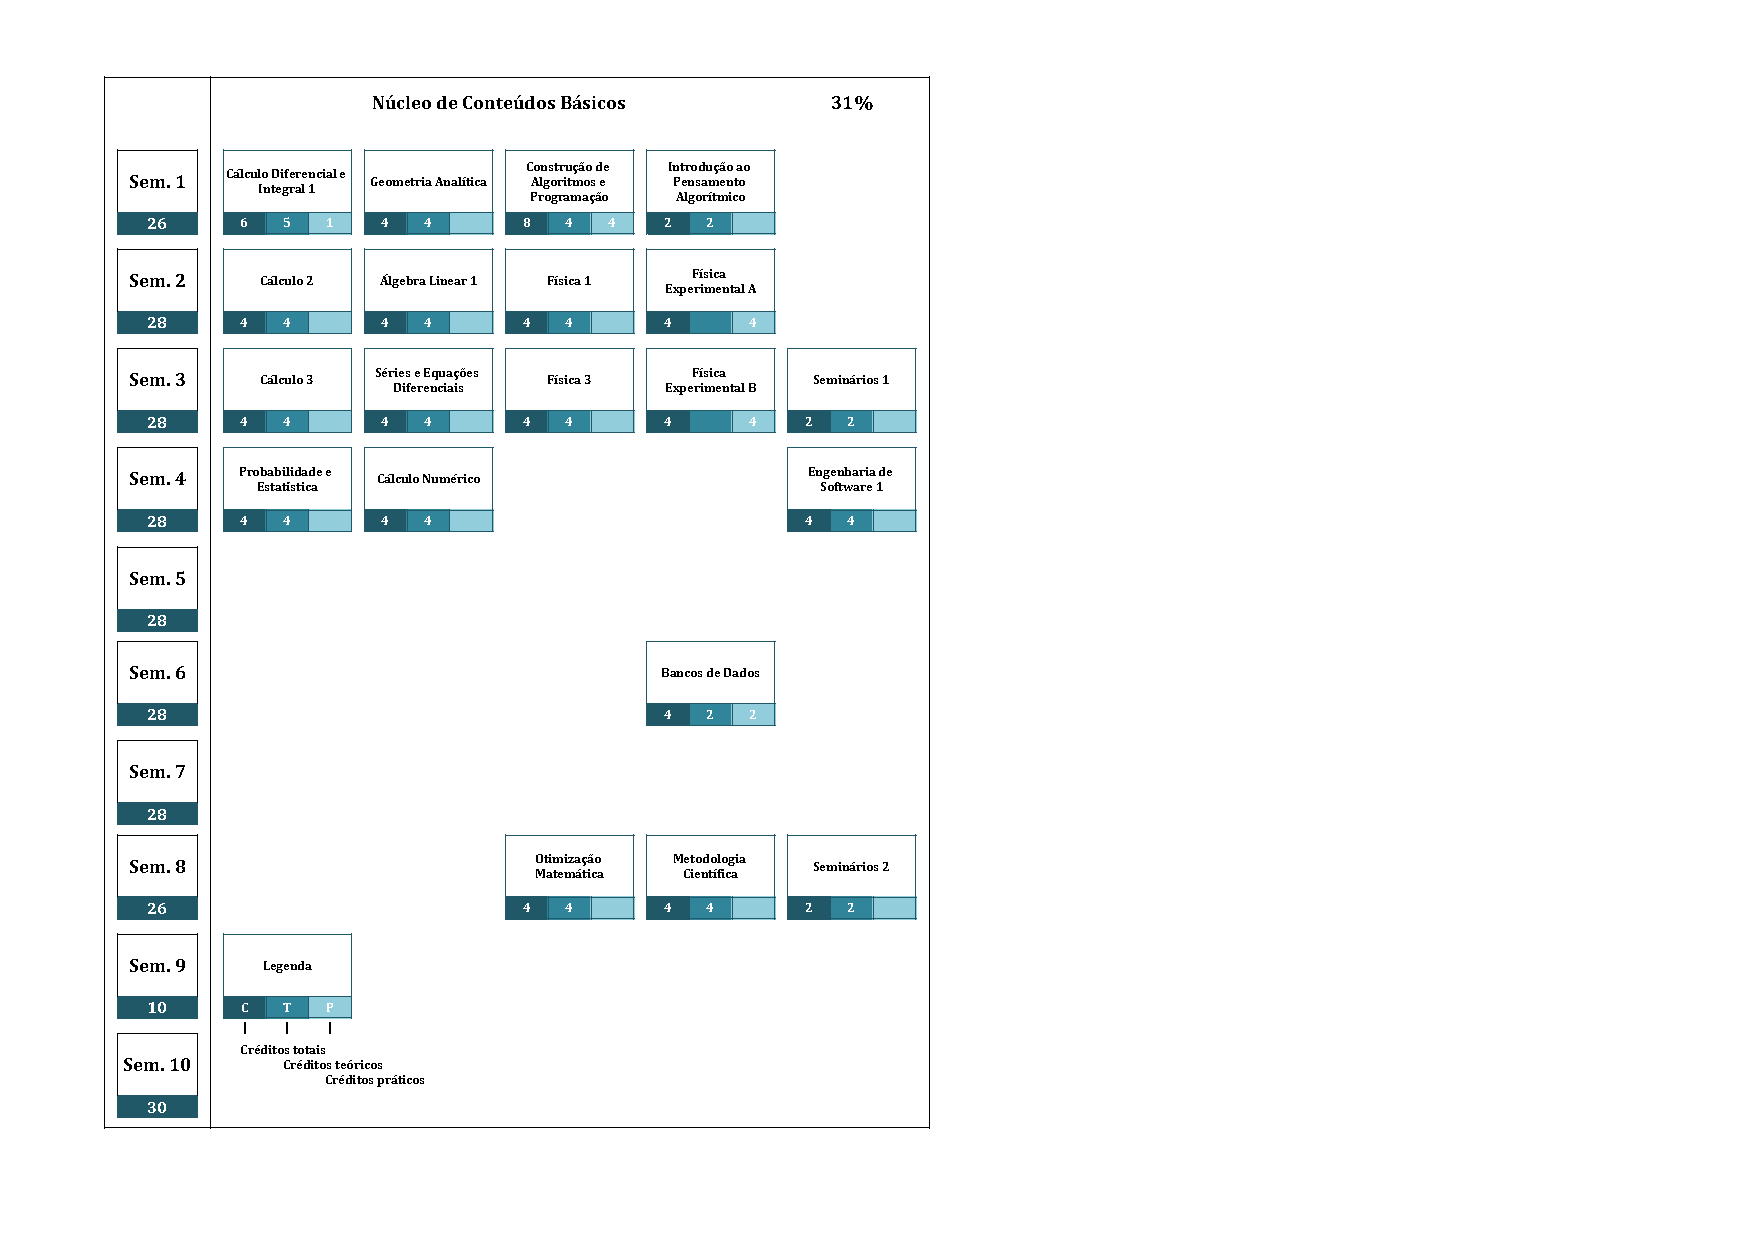
\includegraphics[height=\textwidth]{imagens/Basicos}
% \end{figure}

% %%%%%%%%%%%%%%%%%%%%%%%%%%%%%%%%%%%%%%%%%%%%

% \subsection{Núcleo de Conteúdos Profissionalizantes}~\label{sec:NCP}

% O conteúdo de núcleo de conteúdos profissionalizantes é constituído por 12 disciplinas, que se dividem em diversos tópicos que proporcionam o embasamento necessário para o perfil do egresso.

% Os tópicos Circuitos Elétricos, Controle de Sistemas Dinâmicos, Eletrônica Analógica e Digital e Telecomunicações são abordados nas cinco disciplinas a seguir. Estas disciplinas apresentam teorias e técnicas que permitem o desenvolvimento e análise de projeto e de componentes de sistemas computacionais e de comunicação.

% \begin{compenum}
% \item Circuitos Elétricos
% \item Circuitos Eletrônicos 1
% \item Circuitos Eletrônicos 2
% \item Sistemas Dinâmicos
% \item Tecnologia de Comunicação
% \end{compenum}

% Os tópicos Algoritmos e Estrutura de Dados e Sistemas Operacionais são abordados nas três disciplinas a seguir, e que tem como objetivo capacitar o {estudante} para desenvolver e/ou utilizar ferramentas e técnicas de algoritmos e programação, bem como a formação básica para desenvolvimento de programas que usem eficientemente os recursos e serviços providos por sistemas operacionais tornando os aptos a entender e atuar em desenvolvimento de projeto.

% \begin{compenum}
% \item Algoritmos e Estrutura de Dados 1
% \item Algoritmos e Estrutura de Dados 2
% \item Sistemas Operacionais
% \end{compenum}

% Os tópicos de Circuitos Lógicos e Organização de Computadores são constituídos por quatro disciplinas que tratam à construção de sistemas computacionais, em específico aspectos de \textit{hardware}.

% \begin{compenum}
% \item Lógica Digital
% \item Sistemas Digitais
% \item Arquitetura e Organização de Computadores 1
% \item Arquitetura e Organização de Computadores 2
% \end{compenum}

% Na Figura~\ref{fig:profissionalizantes} apresenta-se o núcleo de conteúdos profissionalizantes e suas componentes curriculares, bem como os respectivos semestres de oferecimento ao longo do curso.

% \begin{figure}[H]
%     \centering
%     \caption{Núcleo de Conteúdos Profissionalizantes}
%     \label{fig:profissionalizantes}
%     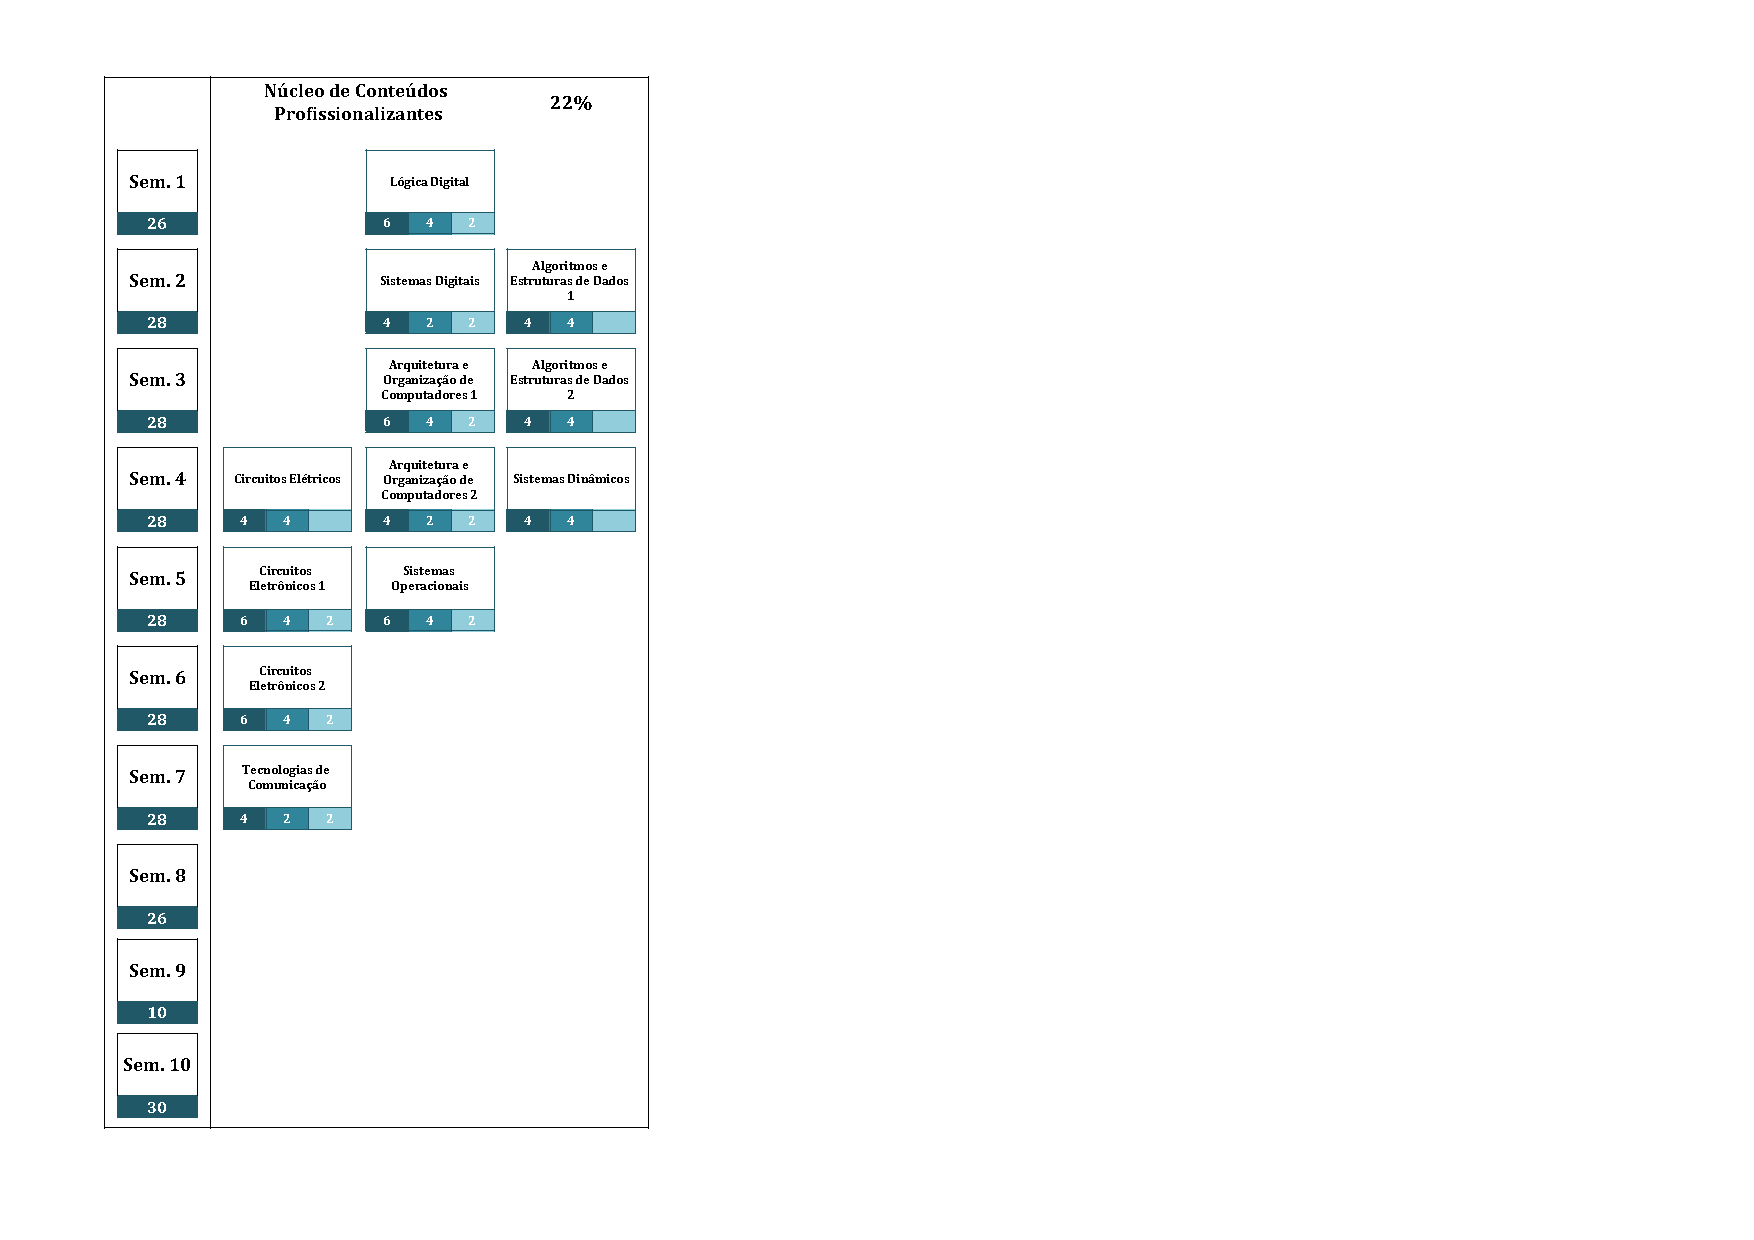
\includegraphics[height=\textwidth]{imagens/Profissionalizantes}
% \end{figure}

% %%%%%%%%%%%%%%%%%%%%%%%%%%%%%%%%%%%%%%%%%%

% \subsection{Núcleo de Conteúdos Específicos}~\label{sec:NCE}

% De acordo com parágrafo 4º - Artº. 6 da Resolução CNE/CES 11/2002, o núcleo de conteúdos específicos se constitui em extensões e aprofundamentos dos conteúdos do núcleo de conteúdos profissionalizantes, bem como de outros conteúdos destinados a caracterizar o curso de Engenharia de Computação. Tendo como objetivo, proporcionar conhecimentos científicos, tecnológicos e instrumentais necessários para a definição do perfil do Bacharel em Engenharia de Computação e garantir o desenvolvimento das competências e habilidades estabelecidas nas diretrizes. Desta forma, este núcleo constitui 24 disciplinas agrupadas em modalidades de conhecimento.

% As cinco disciplinas a seguir, apresentam o aprofundamento da capacitação do {estudante} para desenvolver e aplicar estratégias algorítmicas avançadas, construção de programas verificando a análise e correção do desempenho dos algoritmos, sistemas paralelos e concorrência, consolidação de paradigmas de projeto de algoritmos, avaliação das técnicas a serem implementadas em cada projeto/sistema, bem como projetar e entender tipos de arquiteturas de computadores não convencionais para alto desempenho.

% \begin{compenum}
% \item Programação Orientada a Objetos
% \item Projeto e Análise de Algoritmos
% \item Organização e Recuperação da Informação
% \item Programação Paralela e Distribuída
% \item Arquitetura de Alto Desempenho
% \end{compenum}

% As quatro disciplinas a seguir, apresentam as principais metodologias e técnicas da área da computação, tornando o estudante apto a realizar o \textit{design}, construção e avaliação de sistemas computacionais, bem como o uso de técnicas para prover comunicação, sincronização e coordenação entre múltiplos sistemas de computação distribuídos.

% \begin{compenum}
% \item Redes de Computadores
% \item Sistemas Distribuídos
% \item Interação Humano-Computador
% \item Inteligência Artificial
% \end{compenum}

% Estas nove disciplinas fornecem o conhecimento sobre identificar, formular e avaliar problemas de Engenharia de Computação e conceber soluções, bem como as disciplinas de apoio e prática profissional ao estudante, atividades relacionadas ao desenvolvimento de projetos sob supervisão docente e estágio.

% \begin{compenum}
% \item Controle 1
% \item Controle 2
% \item Processamento de Sinais Digitais
% \item Engenharia de Sistemas
% \item Projeto de Sistemas Computacionais Embarcados
% \item Trabalho de Conclusão de Curso 1
% \item Trabalho de Conclusão de Curso 2
% \item Estágio Supervisionado
% \end{compenum}

% As cinco disciplinas Optativas e Eletivas fornecem aprofundamento em determinadas áreas específicas, permitindo ao estudante optar por um aprofundamento que se adapte a suas habilidades ou demandas específicas de mercado.
% Importante ressaltar, que de acordo com o Regimento Geral dos Cursos de Graduação, Set. 2016 UFSCar (Seção II, Art. 14º)~\cite{RGCG}, devemos assegurar ao estudante a possibilidade de se especializar em Língua Brasileira de Sinais  (LIBRAS) cursando uma disciplina do tipo Optativa, desde o primeiro semestre do curso. A lista das disciplinas optativas está relacionada na Seção~\ref{sec:matriz_curricular}. Estas disciplinas devem ser idealmente cursadas entre o sétimo e nono período, mas podem ser antecipadas, desde que satisfeitos os pré-requisitos. A posição na grade e o número de disciplinas, portanto, é apenas uma sugestão. O estudante pode, por exemplo, cursar duas disciplinas de dois créditos ao invés de uma disciplina de quatro créditos como indicado na Figura~\ref{fig:especificos}.

% \begin{compenum}
% \item Optativa
% \item Optativa
% \item Optativa
% \item Eletiva
% \item Eletiva
% \end{compenum}

% As Atividades Complementares contemplam atividades acadêmicas, científicas e culturais que fazem parte da vida acadêmica do estudante e estão relacionadas com o desenvolvimento das habilidades e atitudes necessárias ao exercício de sua futura profissão. Dentre estas atividades podemos citar atuação em projetos de Iniciação Científica e de extensão universitária; monitorias e tutorias;  disciplinas ACIEPEs (Atividades Curriculares de Integração Ensino, Pesquisa e Extensão); participação na Empresa Júnior e no Programa de Ensino Tutorial da Engenharia de Computação (PET EnC), que é vinculado ao Departamento de Computação. %TODO As regras para consignação das horas-aula de atividades acadêmico-científico-culturais serão determinadas pelo Conselho de Coordenação de Curso, que atualizará quando necessário.

% \begin{compenum}
% \item Atividade Complementar
% \item Atividade Complementar
% \end{compenum}


% Na Figura~\ref{fig:especificos} apresenta-se o núcleo de conteúdos especifícos e suas componentes curriculares, bem como os respectivos semestres de oferecimento ao longo do curso.


% \begin{figure}[H]
%     \centering
%     \caption{Núcleo de Conteúdos Específicos}
%     \label{fig:especificos}
%     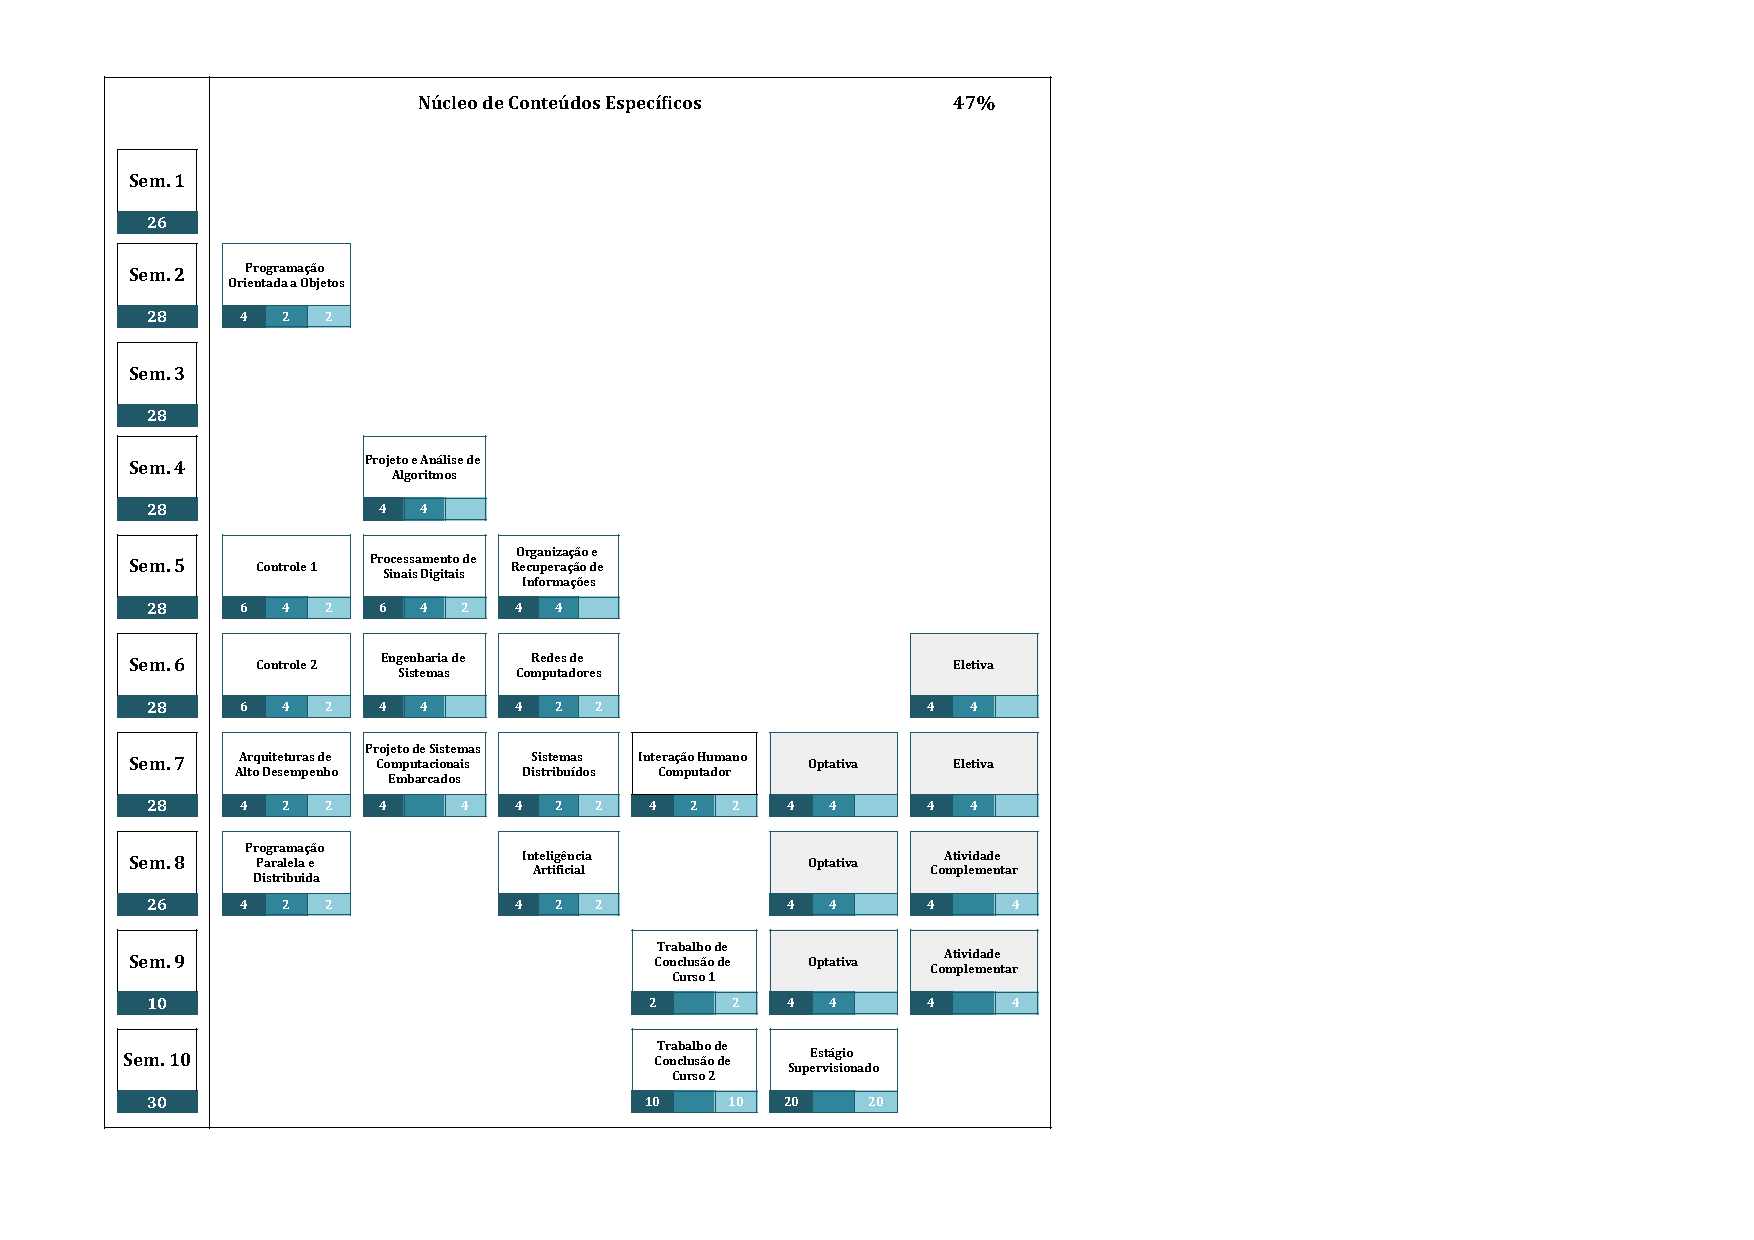
\includegraphics[height=\textwidth]{imagens/Especificos}
% \end{figure}


% \end{comment}

%%%%%%%%%%%%%%%%%%%%


Conforme mencionado, os componentes curriculares foram divididos em conteúdos básicos e tecnológicos referentes à área da computação e conteúdos básicos e tecnológicos específicos para o curso de Engenharia de Computação. Os conteúdos serão apresentados por eixos que agrupam vários componentes curriculares, e estes serão detalhados nas subseções a seguir.
O curso possui a proporção da carga horária apresentada a seguir, bem como, apresenta o subconjunto coerente de tópicos para cada núcleo caracterizando a modalidade do curso.

Para este curso temos a carga total de 3.660 horas de atividades, estando divididas conforme as diretrizes CNE/CES 5/2016 e o Regimento Geral dos Cursos de Graduação da UFSCar~\cite{RGCG}, onde:
%TODO: incluir referência

\begin{compenum}
    \item 57\%, correspondente a 2.070 horas didáticas, aplicado ao núcleo de conteúdos básicos e tecnológicos referentes à área da computação;
    \item 43\%, correspondente a 1.590 horas, aplicado ao núcleo de conteúdos tecnológicos específicos para o curso de Engenharia de Computação. Nesse núcleo estão contemplados:
    \begin{itemize}
        \item 120 horas - Trabalho de Conclusão de Curso;
        \item 180 horas - Estágio Supervisionado;
        \item  60 horas - Atividade Complementar.
    \end{itemize}
\end{compenum}

A seguir são apresentados os componentes curriculares pertencentes a cada eixo. A matriz curricular é apresentada na Seção~\ref{sec:matriz_curricular}.

\subsection{Conteúdos básicos e tecnológicos referentes à área da computação}~\label{sec:cb_tac}

O núcleo de conteúdos básicos e tecnológicos referentes à área da computação é constituído por 5 eixos.

\subsubsection{Eixo de Fundamentos de Matemática e Estatística}~\label{sec:E1}

Este eixo é constituído por sete disciplinas básicas de matemática e uma de estatística, comuns a todos os cursos de ciências exatas e engenharias, que fornencem os conhecimentos básicos na resolução de problemas em engenharia. As disciplinas deste eixo são apresentadas a seguir, bem como os respectivos semestres de oferecimento ao longo do curso.

\begin{compenum}
    \item Cálculo Diferencial e Integral 1 (1º Sem.)
    \item Geometria Analítica (1º Sem.)
    \item Cálculo Diferencial e Integral 2 (2º Sem.)
    \item Álgebra Linear 1 (2º Sem.)
    \item Cálculo 3 (3º Sem.)
    \item Séries e Equações Diferenciais (3º Sem.)
    \item Probabilidade e Estatística (4º Sem.)
    \item Cálculo Numérico (4º Sem.)
\end{compenum}

\subsubsection{Eixo de Algoritmos e Programação}~\label{sec:E4}

Nesse eixo, tem-se oito disciplinas de programação, que enquadram-se como técnicas essenciais na área da computação e apresentam o aprofundamento da capacitação do {estudante} para desenvolver e aplicar estratégias algorítmicas avançadas, construção de programas verificando a análise e correção do desempenho dos algoritmos, sistemas paralelos e concorrência, consolidação de paradigmas de projeto de algoritmos, avaliação das técnicas a serem implementadas em cada projeto/sistema.
% e tem como objetivo capacitar o {aluno} para desenvolver e/ou utilizar ferramentas e técnicas de algoritmos e programação.
As disciplinas Algoritmos e Estrutura de Dados 1 e 2 têm como objetivo capacitar o {estudante} para desenvolver e/ou utilizar ferramentas e técnicas de algoritmos e programação, bem como a formação básica para desenvolvimento de programas que usem eficientemente os recursos e serviços providos por sistemas operacionais tornando-os aptos a entender e atuar em desenvolvimento de projeto.

\begin{compenum}
    \item Construção de Algoritmos e Programação (1º Sem.)
    \item Introdução ao Pensamento Algorítmico (1º Sem.)
    \item Algoritmos e Estrutura de Dados 1 (2º Sem.)
    \item Programação Orientada a Objetos (2º Sem.)
    \item Algoritmos e Estrutura de Dados 2 (3º Sem.)
    \item Projeto e Análise de Algoritmos (4º Sem.)
    \item Organização e Recuperação da Informação (5º Sem.)
    \item Programação Paralela e Distribuída (8º Sem.)
\end{compenum}

\subsubsection{Eixo de Arquiteturas de Computadores}~\label{sec:E5}

Esse eixo é constituído por cinco disciplinas que tratam da construção de sistemas computacionais, em específico aspectos de \textit{hardware}. As disciplinas que compõem este eixo são apresentadas a seguir.

\begin{compenum}
    \item Lógica Digital (1º Sem.)
    \item Sistemas Digitais (2º Sem.)
    \item Arquitetura e Organização de Computadores 1 (3º Sem.)
    \item Arquitetura e Organização de Computadores 2 (4º Sem.)
    \item Arquiteturas de Alto Desempenho (7º Sem.)
\end{compenum}

\subsubsection{Eixo de Metodologia e Técnicas da Computação }~\label{sec:E6}

Este eixo é constituído por sete disciplinas e apresentam as principais metodologias e técnicas da área da computação, tornando o estudante apto a realizar o \textit{design}, construção e avaliação de sistemas computacionais, bem como o uso de técnicas para prover comunicação, sincronização e coordenação entre múltiplos sistemas de computação distribuídos.
As disciplinas que compõem este eixo são apresentadas a seguir.

\begin{compenum}
    \item Engenharia de Software 1 (4º Sem.)
    \item Sistemas Operacionais (5º Sem.)
    \item Banco de Dados (6º Sem.)
    \item Inteligência Artificial (6º Sem.)
    \item Redes de Computadores (7º Sem.)
    \item Sistemas Distribuídos (7º Sem.)
    \item Interação Humano-Computador (8º Sem.)
\end{compenum}

\subsubsection{Eixo de Humanas}~\label{sec:E8}

% Neste eixo, as disciplinas Seminários 1 e Seminários 2 são propostas em um formato alternativo. Diferentemente, em vez de adotar uma disciplina associada a um único núcleo de conhecimento, tais disciplinas tratam núcleos de conhecimentos distintos, trazendo intrinsecamente a vantagem da multidisciplinaridade, que possibilita cativar pela expectativa da contínua novidade, e também, da flexibilidade, que possibilita a modulação dos temas de acordo com os diversos parâmetros envolvidos, por exemplo: audiência e tendências afins mais presentes no quotidiano. Tais  conteúdos são trabalhados na forma de seminários isolados ou programados em série. Estas disciplinas têm como objetivo geral contribuir para a  formação do perfil do futuro profissional nos aspectos, grosso modo, não tecnológicos do curso, alguns explicitados na Resolução CNE/CES 11, de 11 de março de 2002 \footnote{A resolução CNE/CES 11/2002 foi publicada no Diário Oficial da União em 9 de abril de 2002, Seção 1, p.32} a qual trata das Diretrizes Gerais para os cursos de Engenharia,  entre outros:  sociais, profissionais, legais, éticos, políticos e humanísticos. Desta forma, assenta-se a clara preocupação de formar um profissional não somente voltado às competências de suas atividades específicas, mas também torná-lo, de um lado, reflexivo diante de temas gerais importantes para o desenvolvimento da teia social; e, complementarmente, de outro lado, assumir a co-responsabilidade nos rumos seguidos pela sociedade no qual está inserido quando premido pela necessidade de apresentar, em momentos de decisão em face de múltiplas opções, aquela de maior valor coletivo.

Apresentam-se nesse eixo as disciplinas Seminários 1 e 2 que visam trabalhar conteúdos relacionados a Administração, Economia, Humanidades, Ciências Sociais e Cidadania. Em vez de adotar uma disciplina associada a uma única temática, tais disciplinas tratam de conhecimentos distintos, trazendo intrinsecamente a vantagem da multidisciplinaridade, que possibilita cativar pela expectativa da contínua novidade, e também, da flexibilidade, que possibilita a modularização dos temas.

Tais conteúdos são trabalhados na forma de seminários isolados ou programados em série, conforme ementa das respectivas disciplinas. Estas disciplinas têm como objetivo geral contribuir para a formação do perfil do futuro profissional nos aspectos não tecnológicos do curso, explicitados na Resolução CNE/CES 5/2016, tais como sociais, profissionais, legais, éticos, políticos e humanísticos. Desta forma, assenta-se a clara preocupação de formar um profissional não somente voltado às competências técnicas de suas atividades específicas, mas também torná-lo reflexivo diante de temas gerais importantes para o desenvolvimento da sociedade e do bem comum.

\begin{compenum}
    \item Seminários 1 (3º Sem.)
    \item Disciplina Eletiva (6º Sem.)
    \item Disciplina Eletiva (7º Sem.)
    \item Seminários 2 (8º Sem.)
    \item Atividade Complementar (9º Sem.)
\end{compenum}

As Atividades Complementares contemplam atividades acadêmicas, científicas e culturais que fazem parte da vida acadêmica do estudante e estão relacionadas com o desenvolvimento das habilidades e atitudes necessárias ao exercício de sua futura profissão. Dentre estas atividades podemos citar atuação em projetos de Iniciação Científica e de extensão universitária; monitorias e tutorias; disciplinas ACIEPEs (Atividades Curriculares de Integração Ensino, Pesquisa e Extensão); participação na Empresa Júnior e no Programa de Ensino Tutorial da Engenharia de Computação (PET EnC), que é vinculado ao Departamento de Computação. %TODO As regras para consignação das horas-aula de atividades acadêmico-científico-culturais serão determinadas pelo Conselho de Coordenação de Curso, que atualizará quando necessário.

\subsection{Conteúdos básicos e tecnológicos específicos para o curso de Engenharia de Computação}~\label{sec:cb_tec}

O núcleo de conteúdos básicos e tecnológicos específicos para o curso de Engenharia de Computação é constituído em extensões e aprofundamentos dos conteúdos deste núcleo, bem como de outros conteúdos destinados a caracterizar o curso de Engenharia de Computação. Tendo como objetivo proporcionar conhecimentos científicos, tecnológicos e instrumentais necessários para a definição do perfil do Bacharel em Engenharia de Computação e garantir o desenvolvimento das competências e habilidades estabelecidas nas diretrizes. Desta forma, este núcleo constitui quatro eixos que se dividem em diversos tópicos que proporcionam o embasamento necessário para o perfil do egresso.

\subsubsection{Eixo de Física}~\label{sec:E2}

Este eixo é constituído por quatro disciplinas básicas de física, comuns a todos os curso de ciências exatas e engenharias. As disciplinas deste eixo são apresentadas a seguir, bem como os respectivos semestres de oferecimento ao longo do curso.

\begin{compenum}
    \item Física 1 (2º Sem.)
    \item Física Experimental A (2º Sem.)
    \item Física 3 (3º Sem.)
    \item Física Experimental B (3º Sem.)

\end{compenum}

\subsubsection{Eixo de Eletrônica}~\label{sec:E3}

Este eixo é constituído por três disciplinas que apresentam teoria e técnicas que permitem o desenvolvimento, análise e projeto de componentes que compõem sistemas computacionais. As disciplinas deste eixo são apresentadas a seguir, bem como os respectivos semestres de oferecimento ao longo do curso.

\begin{compenum}
    \item Circuitos Elétricos (4º Sem.)
    \item Circuitos Eletrônicos 1 (5º Sem.)
    \item Circuitos Eletrônicos 2 (6º Sem.)
\end{compenum}

\subsubsection{Eixo de Engenharia e Sistemas}~\label{sec:E7}

Este eixo é constituído por doze disciplinas que fornecem o conhecimento sobre identificar, formular e avaliar problemas de engenharia de computação e conceber soluções, bem como as disciplinas de apoio e prática profissional do estudante, atividades relacionadas ao desenvolvimento de projetos sob supervisão docente e estágio. Estas disciplinas também apresentam teorias e técnicas que permitem o desenvolvimento e análise de projeto e de componentes de sistemas computacionais e de comunicação. A disciplina de Otimização Matemática gera a capacitação para resolução de problemas em engenharia de forma analítica e computacional. As disciplinas que compõem este eixo são apresentadas a seguir.

\begin{compenum}
    \item Sistemas Dinâmicos (4º Sem.)
    \item Controle 1 (5º Sem.)
    \item Processamento de Sinais Digitais (5º Sem.)
    \item Controle 2 (6º Sem.)
    \item Engenharia de Sistemas (6º Sem.)
    \item Tecnologia de Comunicação (7º Sem.)
    \item Projeto de Sistemas Computacionais Embarcados (7º Sem.)
    \item Otimização Matemática (8º Sem.)
    \item Metodologia Científica (8º Sem.)
    \item Trabalho de Conclusão de Curso 1 (9º Sem.)
    \item Trabalho de Conclusão de Curso 2 (10º Sem.)
    \item Estágio Supervisionado (10º Sem.)
\end{compenum}

\subsubsection{Eixo de Especializações }~\label{sec:E9}

Este eixo engloba as Disciplinas Optativas que fornecem especializações em determinadas áreas, permitindo que o estudante se adapte às suas habilidades ou a demandas específicas do mercado.

\begin{compenum}
    \item Disciplina Optativa (7º Sem.)
    \item Disciplina Optativa (8º Sem.)
    \item Disciplina Optativa (9º Sem.)

\end{compenum}

É importante ressaltar que, de acordo com o Regimento Geral dos Cursos de Graduação, Set. 2016 UFSCar (Seção II, Art. 14º)~\cite{RGCG}, deve-se assegurar ao estudante a possibilidade de se especializar na Língua Brasileira de Sinais (LIBRAS) cursando uma disciplina do tipo Optativa, desde o primeiro semestre do curso. A lista das disciplinas optativas está relacionada na Seção~\ref{sec:matriz_curricular}. Estas disciplinas devem ser idealmente cursadas entre o sétimo e nono período, mas podem ser antecipadas, desde que satisfeitos os pré-requisitos. A posição na grade e o número de disciplinas, portanto, é apenas uma sugestão. O estudante pode, por exemplo, cursar duas disciplinas de dois créditos ao invés de uma disciplina de quatro créditos.% como indicado na Figura~\ref{fig:especificos}.%TODO Menotti verificar está figura pra esta nova atribuição


\subsection{Atividades Curriculares Extensionista}\label{sec:atividades-curriculares-extensionistas}

De acordo com a Resolução QUE AINDA NÃO SAIU, Art.~5º, as Atividades Curriculares Extensionista (ACEs) que contemplam os princípios listados no artigo Art.~2º, conforme validação pela Comissão Mista ProGrad/ProEx/CoG/Coex, podem ser dos tipos de I a III, a seguir:

\begin{enumerate}[label = \Roman*--]
    \item Ações de extensão, com ou sem bolsa, com aprovação registrada na Pró-Reitoria de Extensão nas modalidades de projetos, cursos, oficinas, eventos e prestação de serviços;
    \item Atividades Curriculares de Integração entre Ensino, Pesquisa e Extensão (ACIEPEs); e
    \item Atividades curriculares com carga horária integral ou parcial voltada à abordagem extensionista.
\end{enumerate}

O Curso de Engenharia de Computação destina um mínimo de 336~horas para estas atividades alocadas em disciplinas com caráter extensionista. Tais disciplinas podem ser caracterizadas dentre as obrigatórias contidas no projeto pedagógico e as optativas.

Disciplinas elencadas: Engenharia de Sistemas, Sistemas Distribuídos, Sistemas Embarcados...

Disciplinas optativas (carga horária de 300 horas): Devem seguir o seguinte template:




\subsection{Matriz Curricular}~\label{sec:matriz_curricular}


A matriz curricular completa é apresentada na Figura~\ref{fig:matriz_completa}. O detalhamento das disciplinas em cada semestre é apresentado nos Quadros~\ref{tab:matriz1} a~\ref{tab:matriz_optativas9}. O Semestre 9, apresentado no Quadro~\ref{tab:matriz9}, possui uma quantidade de créditos reduzida para que o estudante possa: (i) antecipar o início do Estágio Supervisionado e realizá-lo durante um ano, requisito desejável em muitas vagas; (ii) se envolver em Atividades Complementares mais intensas, se assim desejar, e; (iii) cumprir eventuais dependências, se necessário, para se dedicar integralmente ao Estágio Supervisionado e ao Trabalho de Conclusão de Curso.


%%%%%%% Matriz Completa  %%%%%%%%%%%%%%%%%%%
\begin{landscape}
    \begin{figure}[H]
        \centering
        \caption{Matriz Curricular}
        \label{fig:matriz_completa}
        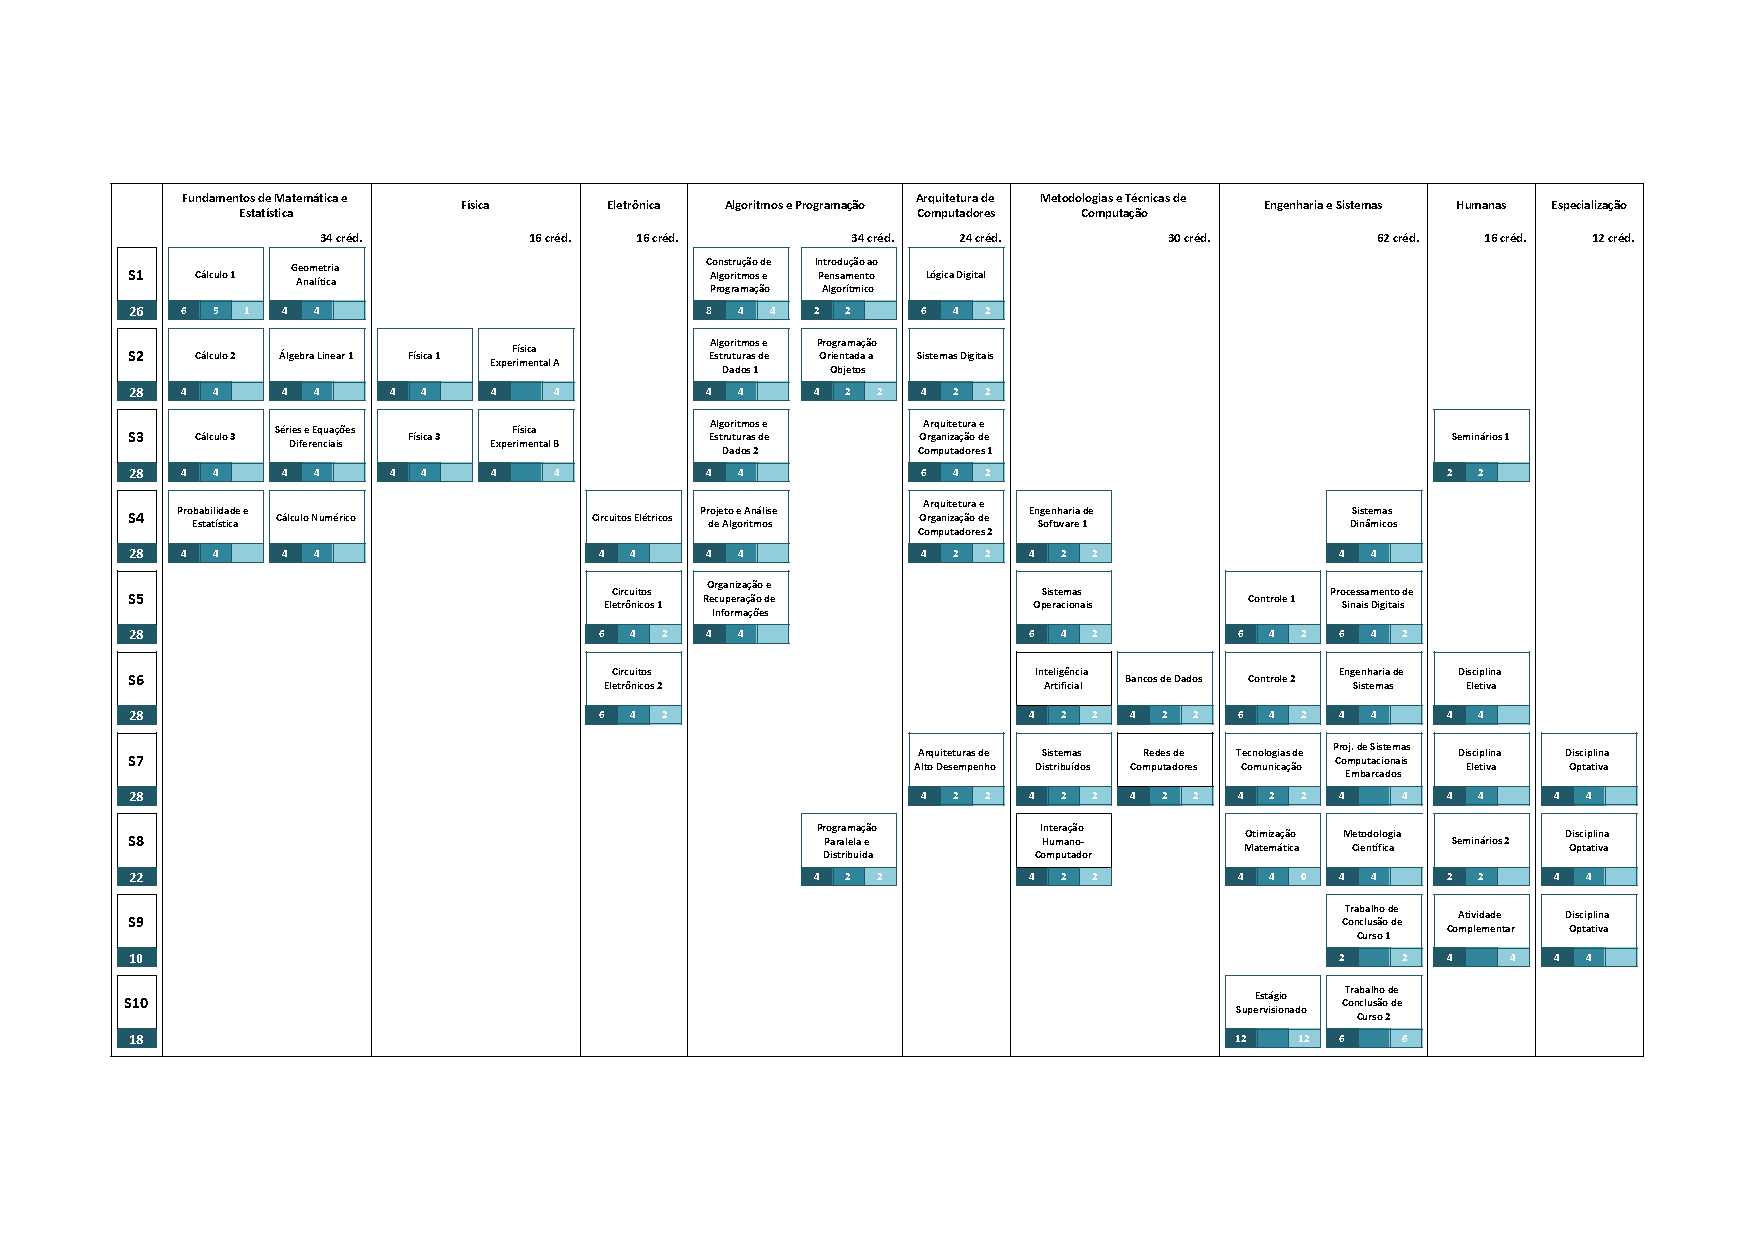
\includegraphics[scale=.9]{imagens/Grade_eixos}
    \end{figure}

    \singlespacing

    % As tabelas abaixo estão na ordem em que aparecem na matriz completa, da esquerda para a direita.
    %%%%%%%%%%%%%%%%%%
    %% Semestre 1: %%%
    %%%%%%%%%%%%%%%%%%

    \begin{table}[H]%[!ht]
        \caption{Matriz Curricular - Semestre 1}
        \centering
        %\footnotesize
        \begin{tabular}{cp{7.0cm}p{7.0cm}ccccc}
            \sline
            \multirow{2}{*}{\textbf{Nro.}} & \multirow{2}{*}{\textbf{Disciplina}} & \multirow{2}{*}{\textbf{Requisito}} & \textbf{Depto.} & \multirow{2}{*}{\textbf{Caráter}} & \multicolumn{3}{c}{\textbf{Natureza}} \\
            &                                        & & \textbf{Ofertante} &             & \textbf{T} & \textbf{P} & \textbf{Total} \\
            \hline
            1 & Cálculo Diferencial e Integral 1       & & DM                 & Obrigatório & 5          & 1          & 6              \\
            2 & Geometria Analítica                    & & DM                 & Obrigatório & 3          & 1          & 4              \\
            3 & Construção de Algoritmos e Programação & & DC                 & Obrigatório & 4          & 4          & 8              \\
            4 & Introdução ao Pensamento Algorítmico   & & DC                 & Obrigatório & 2          & --         & 2              \\
            5 & Lógica Digital                         & & DC                 & Obrigatório & 4          & 2          & 6              \\
            \sline
        \end{tabular}
        \label{tab:matriz1}
    \end{table}

    %%%%%%%%%%%%%%%%%%
    %% Semestre 2: %%%
    %%%%%%%%%%%%%%%%%%

    \begin{table}[H]%[!ht]
        \caption{Matriz Curricular - Semestre 2}
        \centering
        %\footnotesize
        \begin{tabular}{cp{7.0cm}p{7.0cm}ccccc}
            \sline
            \multirow{2}{*}{\textbf{Nro.}} & \multirow{2}{*}{\textbf{Disciplina}} & \multirow{2}{*}{\textbf{Requisito}} & \textbf{Depto.} & \multirow{2}{*}{\textbf{Caráter}} & \multicolumn{3}{c}{\textbf{Natureza}} \\
            &                                   &                                        & \textbf{Ofertante} &             & \textbf{T} & \textbf{P} & \textbf{Total} \\
            \hline
            1 & Cálculo 2                         & Cálculo Diferencial e Integral 1       & DM                 & Obrigatório & 3          & 1          & 4              \\
            2 & Álgebra Linear 1                  & Geometria Analítica                    & DM                 & Obrigatório & 3          & 1          & 4              \\
            3 & Física 1                          &                                        & DF                 & Obrigatório & 4          & --         & 4              \\
            4 & Física Experimental A             &                                        & DF                 & Obrigatório & --         & 4          & 4              \\
            5 & Algoritmos e Estrutura de Dados 1 & Construção de Algoritmos e Programação & DC                 & Obrigatório & 4 & -- & 4 \\
            6 & Programação Orientada a Objetos   & Construção de Algoritmos e Programação & DC                 & Obrigatório & 2 & 2 & 4 \\
            7 & Sistemas Digitais                 & Lógica Digital                         & DC                 & Obrigatório & 2          & 2          & 4              \\
            \sline
        \end{tabular}
        \label{tab:matriz2}
    \end{table}

    %%%%%%%%%%%%%%%%%%
    %% Semestre 3: %%%
    %%%%%%%%%%%%%%%%%%

    \begin{table}[H]%[!ht]
        \caption{Matriz Curricular - Semestre 3}
        \centering
        %\footnotesize
        \begin{tabular}{cp{8.0cm}p{6.0cm}ccccc}
            \sline
            \multirow{2}{*}{\textbf{Nro.}} & \multirow{2}{*}{\textbf{Disciplina}} & \multirow{2}{*}{\textbf{Requisito}} & \textbf{Depto.} & \multirow{2}{*}{\textbf{Caráter}} & \multicolumn{3}{c}{\textbf{Natureza}} \\
            &                                             &                                    & \textbf{Ofertante} &             & \textbf{T} & \textbf{P} & \textbf{Total} \\
            \hline
            1 & Cálculo 3                                   & Cálculo 2                          & DM                 & Obrigatório & 3          & 1          & 4              \\
            2 & Séries e Equações Diferenciais              & Cálculo Diferencial e Integral 1   & DM                 & Obrigatório & 3 & 1 & 4 \\
            3 & Física 3                                    & Física 1                           & DF                 & Obrigatório & 4          & --         & 4              \\
            4 & Física Experimental B                       &                                    & DF                 & Obrigatório & --         & 4          & 4              \\
            5 & Algoritmos e Estrutura de Dados 2           & Algoritmos e Estruturas de Dados 1 & DC                 & Obrigatório & 4 & -- & 4 \\
            6 & Arquitetura e Organização de Computadores 1 & Lógica Digital                     & DC                 & Obrigatório & 4          & 2          & 6              \\
            7 & Seminários 1                                &                                    & DC                 & Obrigatório & --         & 2          & 2              \\
            \sline
        \end{tabular}
        \label{tab:matriz3}
    \end{table}

    %%%%%%%%%%%%%%%%%%
    %% Semestre 4: %%%
    %%%%%%%%%%%%%%%%%%

    \begin{table}[H]%[!ht]
        \caption{Matriz Curricular - Semestre 4}
        \centering
        %\footnotesize
        \begin{tabular}{cp{7.0cm}p{7.0cm}ccccc}
            \sline
            \multirow{2}{*}{\textbf{Nro.}} & \multirow{2}{*}{\textbf{Disciplina}} & \multirow{2}{*}{\textbf{Requisito}} & \textbf{Depto.} & \multirow{2}{*}{\textbf{Caráter}} & \multicolumn{3}{c}{\textbf{Natureza}} \\
            &                                             &                                                                                                & \textbf{Ofertante} &             & \textbf{T} & \textbf{P} & \textbf{Total} \\
            \hline
            1 & Probabilidade e Estatística                 &                                                                                                & DEs                & Obrigatório & 4          & --         & 4              \\
            2 & Cálculo Numérico                            & Cálculo Diferencial e Integral 1, Geometria Analítica e Construção de Algoritmos e Programação & DM & Obrigatório & 3 & 1 & 4\\
            3 & Circuitos Elétricos                         & Séries e Equações Diferenciais                                                                 & DC                 & Obrigatório & 4          & --         & 4              \\
            4 & Projeto e Análise de Algoritmos             & Algoritmos e Estruturas de Dados 1                                                             & DC                 & Obrigatório & 4 & -- & 4 \\
            5 & Arquitetura e Organização de Computadores 2 & Arquitetura e Organização de Computadores 1 & DC & Obrigatório & 2 & 2 & 4 \\ % CoC corrigiu 6 -> 4 % Identificado pela prof. Vania
            6 & Engenharia de Software 1                    & Programação Orientada a Objetos                                                                & DC                 & Obrigatório & 4          & --         & 4              \\
            7 & Sistemas Dinâmicos                          & Séries e Equações Diferenciais e Física 1                                                      & DC                 & Obrigatório & 4          & -- & 4 \\
            \sline
        \end{tabular}
        \label{tab:matriz4}
    \end{table}

    %%%%%%%%%%%%%%%%%%
    %% Semestre 5: %%%
    %%%%%%%%%%%%%%%%%%

    \begin{table}[H]%[!ht]
        \caption{Matriz Curricular - Semestre 5}
        \centering
        %\footnotesize
        \begin{tabular}{cp{7.0cm}p{7.0cm}ccccc}
            \sline
            \multirow{2}{*}{\textbf{Nro.}} & \multirow{2}{*}{\textbf{Disciplina}} & \multirow{2}{*}{\textbf{Requisito}} & \textbf{Depto.} & \multirow{2}{*}{\textbf{Caráter}} & \multicolumn{3}{c}{\textbf{Natureza}} \\
            &                                         &                                                                                                                & \textbf{Ofertante} &             & \textbf{T} & \textbf{P} & \textbf{Total} \\
            \hline
            1 & Circuitos Eletrônicos 1                 & Circuitos Elétricos                                                                                            & DC                 & Obrigatório & 4          & 2          & 6              \\
            2 & Organização e Recuperação de Informação & Algoritmos e Estruturas de Dados 1                                                                             & DC                 & Obrigatório & 4 & -- & 4 \\
            3 & Sistemas Operacionais                   & Arquitetura e Organização de Computadores 1                                                                    & DC                 & Obrigatório & 4 & 2 & 6 \\
            4 & Controle 1                              & Sistemas Dinâmicos                                                                                             & DC                 & Obrigatório & 4          & 2          & 6              \\
            5 & Processamento de Sinais Digitais        & Cálculo Diferencial e Integral 1, Geometria Analítica, Álgebra Linear e Construção de Algoritmos e Programação & DC & Obrigatório & 4 & 2 & 6 \\
            \sline
        \end{tabular}
        \label{tab:matriz5}
    \end{table}

    %%%%%%%%%%%%%%%%%%
    %% Semestre 6: %%%
    %%%%%%%%%%%%%%%%%%

    \begin{table}[H]%[!ht]
        \caption{Matriz Curricular - Semestre 6}
        \centering
        %\footnotesize
        \begin{tabular}{cp{7.0cm}p{7.0cm}ccccc}
            \sline
            \multirow{2}{*}{\textbf{Nro.}} & \multirow{2}{*}{\textbf{Disciplina}} & \multirow{2}{*}{\textbf{Requisito}} & \textbf{Depto.} & \multirow{2}{*}{\textbf{Caráter}} & \multicolumn{3}{c}{\textbf{Natureza}} \\
            &                         &                                    & \textbf{Ofertante} &             & \textbf{T} & \textbf{P} & \textbf{Total} \\
            \hline
            1 & Circuitos Eletrônicos 2 & Circuitos Eletrônicos 1            & DC                 & Obrigatório & 4          & 2          & 6              \\
            2 & Inteligência Artificial & Algoritmos e Estruturas de Dados 1 & DC                 & Obrigatório & 2          & 2          & 4              \\
            3 & Banco de Dados          & Algoritmos e Estrutura de Dados 1  & DC                 & Obrigatório & 2          & 2          & 4              \\
            4 & Controle 2              & Controle 1                         & DC                 & Obrigatório & 4          & 2          & 6              \\
            5 & Engenharia de Sistemas  & Engenharia de Software 1           & DC                 & Obrigatório & 4          & --         & 4              \\
            6 & Disciplina Eletiva      &                                    & --                 & Optativo    & --         & --         & 4              \\
            \sline
        \end{tabular}
        \label{tab:matriz6}
    \end{table}

    %%%%%%%%%%%%%%%%%%
    %% Semestre 7: %%%
    %%%%%%%%%%%%%%%%%%

    \begin{table}[H]%[!ht]
        \caption{Matriz Curricular - Semestre 7}
        \centering
        %\footnotesize
        \begin{tabular}{cp{7.0cm}p{7.0cm}ccccc}
            \sline
            \multirow{2}{*}{\textbf{Nro.}} & \multirow{2}{*}{\textbf{Disciplina}} & \multirow{2}{*}{\textbf{Requisito}} & \textbf{Depto.} & \multirow{2}{*}{\textbf{Caráter}} & \multicolumn{3}{c}{\textbf{Natureza}} \\
            &                                               &                                                                      & \textbf{Ofertante} &             & \textbf{T} & \textbf{P} & \textbf{Total} \\
            \hline
            1 & Arquiteturas de Alto Desempenho               & Arquitetura e Organização de Computadores 1                          & DC & Obrigatório & 2 & 2 & 4 \\
            2 & Sistemas Distribuídos                         & Sistemas Operacionais                                                & DC                 & Obrigatório & 4          & --         & 4              \\
            3 & Redes de Computadores                         & Sistemas Operacionais                                                & DC                 & Obrigatório & 4          & --         & 4              \\
            4 & Tecnologias de Comunicação                    & Sistemas Operacionais                                                & DC                 & Obrigatório & 2          & 2          & 4              \\
            5 & Projeto de Sistemas Computacionais Embarcados & Arquitetura e Organização de Computadores 2 e Engenharia de Sistemas & DC & Obrigatório & -- & 4 & 4 \\
            6 & Disciplina Eletiva                            &                                                                      & --                 & Optativo    & --         & --         & 4              \\
            7 & Disciplina Optativa                           &                                                                      & --                 & Optativo    & --         & --         & 4              \\
            \sline
        \end{tabular}
        \label{tab:matriz7}
    \end{table}

    %%%%%%%%%%%%%%%%%%
    %% Semestre 8: %%%
    %%%%%%%%%%%%%%%%%%

    \begin{table}[H]%[!ht]
        \caption{Matriz Curricular - Semestre 8}
        \centering
        %\footnotesize
        \begin{tabular}{cp{7.0cm}p{7.0cm}ccccc}
            \sline
            \multirow{2}{*}{\textbf{Nro.}} & \multirow{2}{*}{\textbf{Disciplina}} & \multirow{2}{*}{\textbf{Requisito}} & \textbf{Depto.} & \multirow{2}{*}{\textbf{Caráter}} & \multicolumn{3}{c}{\textbf{Natureza}} \\
            &                                    &                                        & \textbf{Ofertante} &             & \textbf{T} & \textbf{P} & \textbf{Total} \\
            \hline
            1 & Programação Paralela e Distribuída & Sistemas Operacionais                  & DC                 & Obrigatório & 2          & 2          & 4              \\
            2 & Interação Humano-Computador        & Construção de Algoritmos e Programação & DC                 & Obrigatório & 2 & 2 & 4 \\
            3 & Otimização Matemática              & Cálculo 2                              & DC                 & Obrigatório & --         & 4          & 4              \\
            4 & Metodologia Científica             &                                        & DC                 & Obrigatório & 4          & --         & 4              \\
            5 & Seminários 2                       & Seminários 1                           & DC                 & Obrigatório & --         & 2          & 2              \\
            6 & Disciplina Optativa                &                                        & --                 & Optativo    & --         & --         & 4              \\
            \sline
        \end{tabular}
        \label{tab:matriz8}
    \end{table}

    %%%%%%%%%%%%%%%%%%
    %% Semestre 9: %%%
    %%%%%%%%%%%%%%%%%%

    \begin{table}[H]%[!ht]
        \caption{Matriz Curricular - Semestre 9}
        \centering
        %\footnotesize
        \begin{tabular}{cp{7.0cm}p{7.0cm}ccccc}
            \sline
            \multirow{2}{*}{\textbf{Nro.}} & \multirow{2}{*}{\textbf{Disciplina}} & \multirow{2}{*}{\textbf{Requisito}} & \textbf{Depto.} & \multirow{2}{*}{\textbf{Caráter}} & \multicolumn{3}{c}{\textbf{Natureza}} \\
            &                                  &                        & \textbf{Ofertante} &             & \textbf{T} & \textbf{P} & \textbf{Total} \\
            \hline
            1 & Trabalho de Conclusão de Curso 1 & Metodologia Científica & DC                 & Obrigatório & 2          & --         & 2              \\
            2 & Atividade Complementar           &                        & --                 & Complem.    & --         & --         & 4              \\
            3 & Disciplina Optativa              &                        & --                 & Optativo    & --         & --         & 4              \\
            \sline
        \end{tabular}
        \label{tab:matriz9}
    \end{table}

    %%%%%%%%%%%%%%%%%%
    %% Semestre 10: %%
    %%%%%%%%%%%%%%%%%%

    \begin{table}[H]%[!ht]
        \caption{Matriz Curricular - Semestre 10}
        \centering
        %\footnotesize
        \begin{tabular}{cp{7.0cm}p{7.0cm}ccccc}
            \sline
            \multirow{2}{*}{\textbf{Nro.}} & \multirow{2}{*}{\textbf{Disciplina}} & \multirow{2}{*}{\textbf{Requisito}} & \textbf{Depto.} & \multirow{2}{*}{\textbf{Caráter}} & \multicolumn{3}{c}{\textbf{Natureza}} \\
            &                                  &                                  & \textbf{Ofertante} &             & \textbf{T} & \textbf{P} & \textbf{Total} \\
            \hline
            1 & Estágio Supervisionado           & 200 créditos                     & DC                 & Estágio     & --         & 12         & 12             \\
            2 & Trabalho de Conclusão de Curso 2 & Trabalho de Conclusão de Curso 1 & DC                 & Obrigatório & -- & 6 & 6 \\
            \sline
        \end{tabular}
        \label{tab:matriz10}
    \end{table}

    %TODO verificar esta lista
    O detalhamento das possíveis disciplinas optativas é apresentado nos Quadros~\ref{tab:matriz_optativas7},~\ref{tab:matriz_optativas8}~e~\ref{tab:matriz_optativas9} de acordo com a sugestão do semestre.

    %%%%%%%%%%%%%%%%%%
    %% Optativas:  %%%
    %%%%%%%%%%%%%%%%%%

    \begin{table}[H]%[!ht] %TODO: conferir se está coerente com as ementas
        \caption{Matriz Curricular - Optativas recomendadas para o 7º semestre}
        \centering
        %\footnotesize
        \begin{tabular}{cp{7.0cm}p{7.0cm}ccccc}
            \sline
            \multirow{2}{*}{\textbf{Nro.}} & \multirow{2}{*}{\textbf{Disciplina}} & \multirow{2}{*}{\textbf{Requisito}} & \textbf{Depto.} & \multirow{2}{*}{\textbf{Caráter}} & \multicolumn{3}{c}{\textbf{Natureza}} \\
            &                                              &                                                                      & \textbf{Ofertante} &          & \textbf{T} & \textbf{P} & \textbf{Total} \\
            \hline
            1  & Aprendizado de Máquina 1                     & Inteligência Artificial e Introdução à Probabilidade e Estatística & DC & Optativo & 4 & -- & 4 \\ %Requisito de IA coloca esta no 9o semestre e inviabiliza AM2
            2  & Computação Gráfica                           & Geometria Analítica e Algoritmos e Estruturas de Dados 1             & DC & Optativo & 2 & 2 & 4 \\
            3  & Controle Avançado                            & Controle 2                                                           & DC                 & Optativo & 2          & 2          & 4              \\
            4  & Desenvolvimento de Software para Web 1       & Banco de Dados                                                       & DC                 & Optativo & --         & 4          & 4              \\
            5  & Empreendedores em Informática                &                                                                      & DC                 & Optativo & 4          & --         & 4              \\
            6  & Engenharia de Software 2                     & Engenharia de Software 1                                             & DC                 & Optativo & 4          & --         & 4              \\
            7  & Introdução à Língua Brasileira de Sinais     &                                                                      & DPsi               & Optativo & 2          & --         & 2              \\
            8  & Lógica Matemática                            &                                                                      & DC                 & Optativo & 4          & --         & 4              \\
            9  & Matemática Discreta                          &                                                                      & DC                 & Optativo & 4          & --         & 4              \\
            10 & Processamento Digital de Imagens & Construção de Algoritmos e Programação, Cálculo Diferencial e Integral I e
            Geometria Analítica & DC & Optativo & 2 & 2 & 4    \\
            11 & Programação Orientada a Objetos Avançada     & Algoritmos e Estruturas de Dados 1 e Programação Orientada a Objetos & DC & Optativo & 2 & 2 & 4    \\
            12 & Projeto e Implementação de Banco de Dados    & Banco de Dados                                                       & DC                 & Optativo & 2          & 2          & 4              \\
            13 & Prototipação de Sistemas Digitais/Analógicos & Circuitos Eletrônicos 2                                              & DC                 & Optativo & -- & 4    & 4    \\
            \sline
        \end{tabular}
        \label{tab:matriz_optativas7}
    \end{table}

    \begin{table}[H]%[!ht] %TODO: conferir se está coerente com as ementas
        \caption{Matriz Curricular - Optativas recomendadas para o 8º semestre}
        \centering
        %\footnotesize
        \begin{tabular}{cp{7.0cm}p{7.0cm}ccccc}
            \sline
            \multirow{2}{*}{\textbf{Nro.}} & \multirow{2}{*}{\textbf{Disciplina}} & \multirow{2}{*}{\textbf{Requisito}} & \textbf{Depto.} & \multirow{2}{*}{\textbf{Caráter}} & \multicolumn{3}{c}{\textbf{Natureza}} \\
            &                                              &                                                       & \textbf{Ofertante} &          & \textbf{T} & \textbf{P} & \textbf{Total} \\
            \hline
            1  & Aprendizado de Máquina 2                     & Aprendizado Máquina 1                                 & DC                 & Optativo & 4          & --         & 4              \\
            2  & Arquitetura de Software e Padrões            & Engenharia de Software 2                              & DC                 & Optativo & 4          & --         & 4              \\
            3  & Banco de Dados para Ciência de Dados         & Projeto e Implementação de Banco de Dados & DC & Optativo & 2 & 2 & 4    \\
            4  & Desenvolvimento de Software para Web 2       & Desenvolvimento de Software para Web 1                & DC & Optativo & -- & 4 & 4    \\
            5  & Introdução à Computação Musical              &                                                       & DC                 & Optativo & 2          & 2          & 4              \\
            6  & Paradigmas de Linguagens de Programação      & Projeto e Análise de Algoritmos                       & DC                 & Optativo & 2 & 2 & 4    \\
            7  & Processamento Digital de Imagens 3D e Vídeos & Processamento Digital de Imagens                      & DC & Optativo & 2 & 2 & 4    \\
            8  & Processamento e Visualização de Dados        & Computação Gráfica                                    & DC                 & Optativo & 2          & 2          & 4              \\
            9  & Segurança Cibernética                        & Sistemas Operacionais e Arquitetura de Computadores 1 & DC & Optativo & 2 & 2 & 4    \\
            10 & Teoria da Computação                         & Matemática Discreta                                   & DC                 & Optativo & 4          & --         & 4              \\
            \sline
        \end{tabular}
        \label{tab:matriz_optativas8}
    \end{table}

    \begin{table}[H]%[!ht] %TODO: conferir se está coerente com as ementas
        \caption{Matriz Curricular - Optativas recomendadas para o 9º semestre}
        \centering
        %\footnotesize
        \begin{tabular}{cp{7.0cm}p{7.0cm}ccccc}
            \sline
            \multirow{2}{*}{\textbf{Nro.}} & \multirow{2}{*}{\textbf{Disciplina}} & \multirow{2}{*}{\textbf{Requisito}} & \textbf{Depto.} & \multirow{2}{*}{\textbf{Caráter}} & \multicolumn{3}{c}{\textbf{Natureza}} \\
            &                                                &                                                                                         & \textbf{Ofertante} &          & \textbf{T} & \textbf{P} & \textbf{Total} \\
            \hline
            1 & Construção de Compiladores                     & Teoria da Computação e Construção de Algoritmos e Programação& DC & Optativo & 4 & -- & 4    \\
            2 & Desenvolvimento Móvel                          & Desenvolvimento de Software para Web 2                                                  & DC                 & Optativo & --         & 4          & 4              \\
            3 & DevOps                                         & Programação Orientada a Objetos Avançada e Arquitetura e Organização de Computadores 1 & DC & Optativo & -- & 4 & 4    \\
            4 & Introdução à Programação de Robôs Móveis       & Álgebra Linear 1, Geometria Analítica e Probabilidade e Estatística & DC & Optativo & 2 & 2 & 4    \\
            5 & Manipuladores Robóticos                        & Álgebra Linear 1,  Geometria Analítica e Cálculo Diferencial e Integral 1 & DC & Optativo & 2 & 2 & 4    \\
            6 & Processamento de Dados em Escala               & Sistemas Operacionais                                                                   & DC                 & Optativo & 2          & 2          & 4              \\
            7 & Projeto de Manufatura Assistido por Computador & Geometria Analítica                                                                     & DC                 & Optativo & 2 & 2 & 4    \\
            8 & Sistemas de Integração e Automação Industrial  & Controle 1                                                                              & DC                 & Optativo & 1          & 3          & 4              \\
            9 & Visão Computacional                            & Processamento de Sinais Digitais ou (Álgebra Linear e Processamento Digital de Imagens) & DC & Optativo & 2 & 2 & 4    \\
            \sline
        \end{tabular}
        \label{tab:matriz_optativas9}
    \end{table}

\end{landscape}

%TODO Citar disicplinas eletivas


\section{Ementário de Disciplinas}\label{sec:ED}

A seguir são apresentadas, por ordem de semestres, as disciplinas do curso, bem como os objetivos, a ementa, pré-requisitos e bibliografia básica e complementar. % As disciplinas que foram reformuladas, bem como novas disciplinas propostas, constam com código XX.XXX-X indicando que um novo código deverá ser criado para cada uma delas. As disciplinas que possuem código permanecem inalteradas.

\singlespacing

%NOTE: Ordenei por semestres para conferir e coincidir com a ordem que aparece na grade (Menotti)
% \subsection{Conteúdo Básico}

% \newpage

% Sem 1
%Cálculo Diferencial e Integral 1
%Geometria Analítica
%Construção de Algoritmos e Programação
%Introdução ao Pensamento Algorítmico
%Lógica Digital

\disciplina{calculo1}{
    \titulo      {1}{Cálculo Diferencial e Integral 1}
    \objetivo    {Propiciar o aprendizado dos conceitos de limite, derivada e integral de funções de uma variável real. Propiciar a compreensão e o domínio dos conceitos e das técnicas de cálculo diferencial e integral. Desenvolver a habilidade de implementação desses conceitos e técnicas em problemas nos quais eles se constituem os modelos mais adequados. Desenvolver a linguagem matemática como forma universal de expressão da ciência.}
    % \requisitos{}
    \recomendadas{N/A}
    \ementa      {Números reais e funções de uma variável real. Limites e continuidade. Cálculo Diferencial e aplicações. Cálculo integral e aplicações.}
    \creditos{6 total (5 teóricos, 1 prático)}
    %     % \horas    {90 total (75 teóricas, 15 práticas)}
    % %    \extra       {6 horas}
    \codigo      {DM}{08.221-0}
    \bibliografia {
        GUIDORIZZI, H. L. Um curso de cálculo v. 1 – 5a. Edição, Rio de Janeiro: Livros Técnicos e Científicos, 2001.

        STEWART, J. Cálculo v. 1 – 5a. Edição, São Paulo: Pioneira Thomson Learning, 2006.

        SWOKOWSKI, E. W. Cálculo com geometria analítica v. 1 – 2a. Edição, São Paulo: McGraw-Hill do Brasil, 1994.
    }{
        ANTON, H. Cálculo v. 1, 10. ed, Porto Alegre, RS: Bookman, 2014.

        ÁVILA, G. Calculo: funções de uma variável v. 1 - 6a. Edição, Rio de Janeiro: Livros Técnicos e Científicos, 1994.

        FLEMMING, D. M.; GONCALVES, M. B. Cálculo A: funções, limite, derivação, integração – 6a. Edição, São Paulo: Prentice Hall, 2006.

        LEITHOLD, L. O cálculo com geometria analítica v. 1 – 3. ed, São Paulo: Harbra, 1991.

        THOMAS, G. B. et al. Cálculo, v.1 - 10a. Edição, Addison Wesley, 2002.
    }

    % Inserido por Murillo R. P. Homem, em 01/04/2023
     \competencias{
        cg-aprender/{ce-ap-1, ce-ap-2, ce-ap-3, ce-ap-4},
        cg-atuar/{ce-atuar-1, ce-atuar-2, ce-atuar-3, ce-atuar-4},
        }
        
}
  %Cálculo Diferencial e Integral 1
\disciplina{ga}{
    \titulo      {1}{Geometria Analítica}
    \objetivo    {Introduzir linguagem básica e ferramentas (matrizes e vetores), que permitam ao aluno analisar e resolver alguns problemas geométricos, no plano e espaço euclidianos, preparando-o para aplicações mais gerais do uso do mesmo tipo de ferramentas. Mais especificamente: Analisar e resolver problemas elementares que envolvem operações de matrizes e sistemas de equações lineares; Analisar soluções de problemas geométricos no plano e no espaço através do uso de vetores,matrizes e sistemas; Identificar configurações geométricas no plano e no espaço euclidiano a partir de suas equações, bem como deduzir equações para tais configurações. Resolver problemas que envolvem essas configurações.
    }
    % \requisitos  {N/A} % xxxxxxx
    \recomendadas{N/A}
    \ementa      {Matrizes; Sistemas Lineares; Eliminação Euclidiana. Vetores; produto escalar;vetorial e misto. Retas e Plano. Cônicas e Quadráticas.}
    \creditos    {4 total (3 teóricos, 1 práticos)}
    % %    \extra       {x horas}
    \codigo      {DM}{08.111-6}
    \bibliografia {
        BOULOS, P. e CAMARGO, I. Geometria analítica, um tratamento vetorial - 3. ed. - Pearson Editora, 2005.

        CAROLI, A., CALLIOLI, C. A., FEITOSA, M. O. Matrizes, vetores e geometria analitica - Editora Nobel, São Paulo, 1987.

        STEINBRUCH, A., WINTERLE, P. Geometria analítica - 2. ed. , Pearson Editora, São Paulo, 2006.
    }{
        BALDIN, Y. Y. e FURUYA, Y. K. S. Geometria analítica para todos e atividades com Octave e GeoGebra -  São Carlos: EDUFSCa, 2011r.

        CALLIOLI, C. A., DOMINGUES, H. H., COSTA, R. Álgebra linear e aplicações, 6 ed., São Paulo: Atual, 2007.

        LIMA, E. L. Geometria analítica e álgebra Linear - IMPA, 2001.

        LIPSCHUTZ, S. Álgebra linear: teoria e problemas - McGraw-Hill, 1994.

        WINTERLE, PVetores e geometria analítica - Makron Books, 2000.
    }

    % Inserido por Murillo R. P. Homem, em 01/04/2023
     \competencias{
        cg-aprender/{ce-ap-1, ce-ap-2, ce-ap-3, ce-ap-4},
        cg-atuar/{ce-atuar-1, ce-atuar-2, ce-atuar-3, ce-atuar-4},
        }
        
}        %Geometria Analítica
\disciplina{cap}{
    \titulo      {1}{Construção de Algoritmos e Programação}
    \objetivo    {Tornar os estudantes aptos a utilizar pensamento computacional e algorítmico para proposição de soluções de problemas. Capacitar os estudantes a mapear tais soluções em programas usando linguagem de programação.}
    \requisitos  {N/A} % xxxxxxx
    \recomendadas{N/A}
    \ementa      {Noções gerais da computação: organização de computadores, programas, linguagens e aplicações. Detalhamento de algoritmos estruturados e programação: tipos básicos de dados. Representação e manipulação de dados. Estruturas de controle de fluxo (condicionais e repetições). Modularização (sub-rotinas, passagem de parâmetros e escopo). Documentação. Estruturação básica de dados: variáveis compostas heterogêneas (registros) e homogêneas (vetores e matrizes). Operações em arquivos e sua manipulação. Alocação dinâmica de memória e ponteiros.}
    \creditos    {8 total (4 teóricos, 4 práticos)}
    %    \extra       {4 horas}
    \codigo      {DC}{1001350}
    \bibliografia {
        CIFERRI. R.R. Programação de Computadores, Edufscar, 2009.

        MEDINA, M. ; FERTIG. C. Algoritmos e Programação: Teoria e Prática, Novatec, 2005.

        SENNE,  E. Primeiro Curso de Programação em C, Visual Books, 2003.

        TREMBLAY, J.P.; BUNT. R.B. Ciência dos Computadores, McGraw-Hill, 1981.

        KERNIGHAN, B.W. ; RITCHIE, D.M. The C Programming Language (2nd Edition), 1988.
    }{
        HARBISON, S.P.; STEELE., G.L. C: a reference manual, 2002.

        KOCHAN; S.G. Programming in C: A complete introduction to the C programming language, 2004.

        KING,  K.N. C Programming: A Modern Approach, Norton \& Company, 1996.
    }
    % Jander, em 15/2/23
    \dataatualizacao{9/10/23} % Jander, Alexandre, Edilson, Fredy
    \competencias{%
        % Revisto sem modificações
        cg-aprender/{ce-ap-4},
        cg-produzir/{ce-pro-2, ce-pro-4},
        cg-atuar/{ce-atuar-1, ce-atuar-2},
        cg-empreender/{ce-emp-2},
    }
}
       %Construção de Algoritmos e Programação
\disciplina{ipa}{
    \titulo      {1}{Introdução ao Pensamento Algorítmico}
    \objetivo    {Motivar e orientar os estudantes a desenvolver soluções sistemáticas para problemas diversos, contextualizados em situações cotidianas, de modo que estas possam ser implementadas a fim de usar o computador como ferramenta para obtenção de resultados. Desenvolver nos estudantes a habilidade de organizar e analisar dados de um problema, a fim de encontrar soluções utilizando técnicas de abstração, decomposição, reconhecimento de padrões e generalização, além da capacidade de analisar a eficiência de suas soluções.}
    \requisitos  {N/A} % xxxxxxx
    \recomendadas{N/A}
    \ementa      {Introdução ao pensamento algorítmico. Análise e especificação de problemas sob o aspecto de pensamento algorítmico. Técnicas de resolução de problemas: abstração, decomposição, reconhecimento de padrões e generalização. Representação e visualização de dados e soluções, com interpretação de resultados. Noções de paralelização. Noções de eficiência de um algoritmo. Introdução em alto nível de algoritmos de diversas áreas da ciência da computação: ordenação, busca, conectividade em grafos, caminhos mínimos, hashing, k-nn, criptografia.}
    \creditos       {2 total (2 teóricos)}
    %    \extra       {3 horas}
    \codigo      {DC}{1001349}
    \bibliografia {
        BHARGAVA, A. Y. Entendendo Algoritmos: Um guia ilustrado para programadores e outros curiosos. NOVATEC, 2017. 264 p. ISBN 978-85-752-2563-9.

        LOPES, A.; GARCIA, G.. Introdução à programação: 500 algoritmos resolvidos. Rio de Janeiro: Elsevier, 2002. 469 p. ISBN 978-85-352-1019-4.

        SPRAUL, V. A. Think like a programmer: an introduction to creative problem solving. No Starch Press, 2012. 256 p. ISBN 978-1593274245

        SOUZA, M. A. F. Algoritmos e lógica de programação: um texto introdutório para engenharia. 2.ed. São Paulo: Cengage Learning, 2014. 234 p. ISBN 9788522111299.
    }{
        FORBELLONE, A. L. V.; EBERSPACHER, H. F. Lógica de programação: a construção de algoritmos e estruturas de dados. 3. ed. São Paulo: Pearson Prentice Hall, 2008. 218 p. ISBN 978-85-7605-024-7.

        HOLLOWAY, J. P. Introdução a programação para engenharia: resolvendo problemas com algoritmos. Rio de Janeiro: LTC, 2006. 339 p. ISBN 8521614535.

        SKIENA, S. S. The algorithm design manual. New York: Springer-Verlag, c1998. 486 p. ISBN 0-387-94860-0.

        ERWIG, Martin. Once Upon an Algorithm: How Stories Explain Computing. MIT Press, 2017. 336 p. ISBN 978-0262036634

        FILHO, W. F.; PICTET, R. Computer Science Distilled: Learn the Art of Solving Computational Problems. Code Energy, 2017. 183 p. ISBN 0997316004

        TILLMAN, F. A.; CASSONE, D. T. A Professional's Guide to Problem Solving with Decision Science. Pioneering Partnerships LLC, 2018. 298 p. ISBN 978-0999767115
    }
    % Jander, em 15/2/23
    \competencias{
        cg-aprender/{ce-ap-3, ce-ap-4},
        cg-produzir/{ce-pro-2, ce-pro-4},
        cg-atuar/{ce-atuar-1, ce-atuar-2},
        cg-empreender/ce-emp-2,
    }
}       %Introdução ao Pensamento Algorítmico
\disciplina{ld}{
    \titulo      {1}{Lógica Digital}
    \objetivo    {Ao final da disciplina o estudante deve ser capaz de projetar e analisar circuitos digitais combinatórios e sequenciais e executar sua implementação usando circuitos integrados e linguagem de descrição de hardware.}
    \requisitos  {N/A}
    \recomendadas{N/A}
    \ementa      {Conceitos fundamentais de Eletrônica Digital. Representação digital da informação. Álgebra Booleana. Tabelas verdade e portas lógicas. Expressões lógicas e formas canônicas. Estratégias de minimização de circuitos. Elementos de memória. Máquinas de estado (Mealy e Moore). Circuitos funcionais típicos (combinacionais e sequenciais).}
    \creditos    {6 total (4 teóricos, 2 práticos)}
    %    \extra       {3 horas}
    \codigo      {DC}{1001351}
    \bibliografia {
        TOCCI, Ronald J.; WIDMER, Neil S. MOSS, Gregory L. Sistemas digitais: princípios e aplicações. 11. ed. São Paulo: Pearson Prentice Hall, 2011. xx, 817 p. : il. ISBN 9788576059226.

        WAKERLY, John F. Digital design: principles and practices. 4. ed. Upper Saddle River: Pearson Prentice Hall, 2006. 895 p. ISBN 0-13-186389-4.

        FLOYD, Thomas L. Sistemas digitais: fundamentos e aplicações. 9. ed. Porto Alegre, RS: Artmed, 2007. xiii, 888 p. ISBN 9788560031931.
    }{
        Stephen Brown, Zvonko Vranesic, and Brown Stephen; Fundamentals of Digital Logic with Verilog Design; McGraw-Hill Companies,Inc.; Edition 2; 2007.

        PEDRONI, Volnei Antonio. Eletrônica digital moderna e VHDL: princípios digitais, eletrônica digital, projeto digital, microeletrônica e VHDL. Rio de Janeiro: Elsevier, 2010. 619 p. ISBN 9788535234657.

        ERCEGOVAC, Milos D.; LANG, Tomás. Digital arithmetic. San Frascisco: Morgan Kaufmann, c2004. 709 p. ISBN 1-55860-798-6.

        Victor P. Nelson, H. Troy Nagle, Bill D. Carroll, David Irwin; Digital Logic Circuit Analysis and Design; Edition 1
        Prentice Hall; 1995.

        Norman Balabanian e Bradley Carlson; Digital Logic Design Principles; Edition 1; Wiley; 2000.
    }
    \dataatualizacao{23/10/23} % Edilson, Márcio, Luciano, Menotti, Helio, Jander, 
    \competencias
    {
        cg-aprender/{ce-ap-1, ce-ap-2, ce-ap-3},
        cg-produzir/{ce-pro-1, ce-pro-2, ce-pro-4, ce-pro-5},
        cg-atuar/{ce-atuar-1, ce-atuar-2, ce-atuar-3, ce-atuar-4}
    }
}        %Lógica Digital

\ExecuteLista{\Disciplina}{calculo1, ga, cap, ipa, ld}{\MostraDisciplina{\Disciplina}}


% Sem 2
%Cálculo 2
%Álgebra Linear
%Física 1
%Física Experimental A
%Algoritmos e Estruturas de Dados 1
%Programação Orientada a Objetos
%Sistemas Digitais

\disciplina{calculo2}{
    \titulo      {2}{Cálculo 2}
    \objetivo    {Aplicar os critérios de convergência para séries infinitas, bem como expandir funções em série de potências. Interpretar geometricamente os conceitos de funções de duas ou mais variáveis e ter habilidade nos cálculos de derivadas e dos máximos e mínimos de funções. Aplicar os teoremas das funções implícitas e inversas}
    \requisitos  {Cálculo Diferencial e Integral 1} % FAVOR NÃO ALTERAR PARA Cálculo 1, pois não é!!! 82210 OU 89109 OU 344001 OU 524034 OU 344001 OU 342009 OU 342211 OU 340456 OU 341258 OU (82619 E 82627) OU (215171 E 215287) OU (215287 E 215384)
    \recomendadas{N/A}
    \ementa      {Curvas e superfícies. Funções reais de várias variáveis. Diferenciabilidade de funções de várias variáveis. Fórmula de Taylor;  Máximos e mínimos; Multiplicadores de Lagrange. Derivação implícita e aplicações.}
    \creditos    {4 total (3 teóricos, 1 práticos)}
%    \extra       {x horas}
    \codigo      {DM}{08.920-6}
     \bibliografia {
        GUIDORIZZI, H. L. Um curso de cálculo. v. 2 – Livros Técnicos e Científicos, Rio de Janeiro, 2004 
        
        PINTO, D.;  MORGADO, M. C. F. Cálculo diferencial e integral de funções de várias variáveis -  UFRJ/SR-1, 1997. 
        
        THOMAS, G. B. et al. Cálculo, v.2 - 10a. Edição, Addison Wesley, 2003. 
    }{
        ÁVILA, G. S.S. Cálculo: funções de várias variáveis - 3a. Ediçao,  Rio de Janeiro: Livros Tecnicos e Cientificos, 1981. v.3. 258 p.  
        
        LIMA, E. L. Curso de análise v.2 - Projeto Euclides. Rio de Janeiro, IMPA, 1989. 
        
        RUDIN, W. Principles of mathematical analysis - 3. ed - McGraw-Hill, c1976. 
        
        STEWART, J.  Cálculo  v. 2, 4. ed,  Pioneira/Thomson Learning, São Paulo, 2001. 
        
        SWOKOWSKI, E. W. Cálculo com geometria analítica, v. 2 - 2. ed. – Markron Books, 1991.
    }

    % Inserido por Murillo R. P. Homem, em 01/04/2023
     \competencias{
        cg-aprender/{ce-ap-1, ce-ap-2, ce-ap-3, ce-ap-4},
        cg-atuar/{ce-atuar-1, ce-atuar-2, ce-atuar-3, ce-atuar-4},
        }
        
}

\disciplina{algelin}{
    \titulo      {2}{Álgebra Linear}
    \objetivo    {Levar o aluno a entender e reconhecer as estruturas da Álgebra Linear,
        que aparecem em diversas áreas da matemática e, trabalhar com estas estruturas, tanto abstrata como concretamente (através de cálculo com representações matriciais).
    }
    \requisitos  {Geometria Analítica} % 81116 OU (215279 E 215384) OU 343510 OU 342017 OU 342190 OU 81515 OU 345083 OU 345970 OU 524182 % 
    \recomendadas{N/A}
    \ementa      {Espaços Vetoriais; Transformações Lineares; Diagonalização de
    Matrizes; Espaços com Produto Interno; Formas Bilineares e
    Quadráticas.}
    \creditos    {4 total (3 teóricos, 1 práticos)}
    %    \extra       {x horas}
    \codigo      {DM}{08.013-6} % Corrigido CoC DC -> DM % Sabrina 
    \bibliografia{
        BOLDRINI, J. L. et al. Álgebra Linear. 3. ed. São Paulo: Harbra, 1986.

        CALLIOLI, C. A.; DOMINGUES, H. H.; Costa, R. C. F. Álgebra linear e aplicações. 6. ed.São Paulo: Atual, 2013.

        COELHO, F. U.; LOURENÇO, M. L. Um curso de álgebra linear. 2. ed. São Paulo: EdUSP, 2010.
    }{
        ANTON, H.; BUSBY, R. C. Álgebra linear contemporânea. Porto Alegre, RS: Bookman, 2008.

        LIMA, E. L. Álgebra linear. 5. ed. Rio de Janeiro: IMPA. (Coleção Matemática Universitária), 2001.

        HOFFMAN, K.; KUNZE, R. Álgebra linear. 2. ed. Rio de Janeiro: Livros Técnicos e Científicos, 1979.

        LANG, S. Álgebra linear. São Paulo: Edgard Blucher, 1971.

        LIPSCHUTZ, S. Álgebra linear. São Paulo: McGraw-Hill do Brasil, 1973.

        MONTEIRO, L. H. J. Álgebra linear. São Paulo: Nobel, 1970.
    }

    % Inserido por Murillo R. P. Homem, em 01/04/2023
     \competencias{
        cg-aprender/{ce-ap-1, ce-ap-2, ce-ap-3, ce-ap-4},
        cg-atuar/{ce-atuar-1, ce-atuar-2, ce-atuar-3, ce-atuar-4},
        }
        
}

\disciplina{fisica1}{
    \titulo      {2}{Física 1}
    \objetivo    {Introduzir os princípios básicos da Física Clássica (Mecânica), tratados
    de forma elementar, desenvolvendo no estudante a intuição necessária para analisar fenômenos físicos sob os pontos de vista qualitativo e quantitativo. Despertar o interesse e ressaltar a necessidade do estudo desta matéria, mesmo para não especialistas.}
    \requisitos  {N/A} % xxxxxxx
    \recomendadas{N/A}
    \ementa      {Movimento de uma partícula em 1D, 2D e 3D; Leis de Newton; Aplicações das Leis de Newton – Equilíbrio de Líquidos (Arquimedes) - Forças Gravitacionais; Trabalho e Energia; Forças Conservativas – Energia Potencial; Conservação da Energia (Equação de Bernoulli); Sistemas de Várias Partículas – Centro de Massa; Colisões; Conservação do Momento Linear.
    }
    \creditos    {4 total (4 teóricos)}
    %    \extra       {x horas}
    \codigo      {DF}{09.901-5}
    \bibliografia {
        HALLIDAY, D.; RESNICK, R.; WALKER. J. Fundamentos de Física, volume 1, Mecânica, 9ª edição, GEN/LTC 2012.

        YOUNG, H. D.; FRIEDMAN. R. A.; SEARS ; ZEMANSKY. Física I: Mecânica, 12.ed.. Pearson, São Paulo.

        CHAVES,  A.; SAMPAIO,  J.F. Física Básica: Mecânica.
    }{
        NUSSENZVEIG, H.M. Curso de Física Básica, v. 1

        TIPLER,  P. A.; . MOSCA,  G. Física para cientista e engenheiros, v. 1, Mecânica, 6. ed., GEN/LTC, 2008.

        SERWAY R. A.; JEWETT, Jr. J. W. Princípios de Física, v. 1, Mecânica. 3 ed.. Editorial Thomson. 2005.

        FEYNMAN R.P.; Lectures on Physics, v. 1.

        KELLER, F.J.; GETTYS,  W.E.; SKOVE, M.J. Física, v. 1
    }
    % Inserido por Edilson Kato, em 11/03/2024
     \competencias{
        cg-aprender/{ce-ap-1, ce-ap-2, ce-ap-3, ce-ap-4},
        cg-atuar/{ce-atuar-1, ce-atuar-2, ce-atuar-3, ce-atuar-4},
        }
}

\disciplina{fisexpa}{
    \titulo      {2}{Física Experimental A}
    \objetivo    {Treinar o aluno para desenvolver atividades em laboratório. Familiarizá-lo
    com instrumentos de medidas de comprimento, tempo e temperatura. Ensinar o aluno a organizar dados experimentais, a determinar e processar erros, a construir e analisar gráficos, para que possa fazer uma avaliação crítica de seus resultados. Verificar experimentalmente as leis da Física.}
    \requisitos  {N/A} % xxxxxxx
    \recomendadas{N/A}
    \ementa      {Medidas e erros experimentais; Cinemática e dinâmica de partículas; Cinemática e dinâmica de corpos rígidos; Mecânica de meios contínuos;Termometria e calorimetria.}
    \creditos    {4 total (4 práticos)}
    %    \extra       {x horas}
    \codigo      {DF}{09.110-3}
    \bibliografia {
        INMETRO. Avaliação de dados de medição: guia para a expressão de incerteza de medição – GUM 2008. Traduzido de: Evaluation of measurement data: guide to the expression of uncertainty in measurement – GUM 2008. 1ª Ed. Duque de Caxias, RJ: INMETRO/CICMA/SEPIN, 2012. Disponível em:< http://www.inmetro.gov.br/infotec/publicacoes/gum\_final.pdf>. Acesso em: 13 Mar. 2013.

        HALLIDAY, D.; RESNICK, R.; WALKER, J. Fundamentos de Física: mecânica. [Fundamentals of physics]. Gerson Bazo Costamilan (Trad.). 4. ed. Rio de Janeiro: LTC, 1993

        VUOLO, J. H. Fundamentos da Teoria de Erros. 2. ed. São Paulo, SP: Editora Edgard Blücher LTDA
    }{
        INMETRO. Vocabulário internacional de termos fundamentais e gerais de Metrologia: portaria INMETRO nº 029 de 1995. 5. ed. Rio de Janeiro: Editiora SENAI, 2007.

        NUSSENZVEIG, H. M. Curso de Física Básica, 3. ed. São Paulo: Editora Edgard Blücher LTDA, 1996.

        CAMPOS, A. A; ALVES, E.S; SPEZIALI, N.L. Física Experimental Básica na Universidade, 2. ed. Belo Horizonte: Editora UFMG, 2008.

        DUPAS, M. A. Pesquisando e normalizando: noções básicas e recomendações úteis para a elaboração de trabalhos científicos. 6. ed. São Carlos: Editora EdUFSCar, 2009.

        WORSNOP, B. L.; FLINT, H. T. Curso Superior de Física Práctica - Tomo I. Buenos Aires: EUDEBA, 1964.
    }

}

\disciplina{aed1}{
    \titulo      {2}{Algoritmos e Estruturas de Dados 1}
    \objetivo    {Tornar os estudantes aptos a utilizar técnicas básicas de programação em seus projetos; capacitar os estudantes a reconhecer, implementar e modificar algoritmos e estruturas de dados básicos; familiarizar os estudantes com noções de projeto e análise de algoritmos, através do estudo de uma linguagem algorítmica, exemplos e exercícios práticos; estimular os estudantes a avaliar quais técnicas de programação, algoritmos e estruturas de dados se adequam melhor a cada situação, problema ou aplicação.}
    \requisitos  {Construção de Algoritmos e Programação} % xxxxxxx
    \recomendadas{N/A}
    \ementa      {Introdução à recursão, com algoritmos e aplicações. Visão intuitiva sobre análise de correção (invariantes) e eficiência (complexidade) de algoritmos. Apresentação de busca linear e binária. Apresentação de algoritmos de ordenação elementares (insertion sort, selection sort e bubble sort). Apresentação de programação por retrocesso (backtracking) e enumeração. Noções de tipos abstratos de dados. Detalhamento de estruturas de dados como: listas (alocação estática e dinâmica, circulares, duplamente ligadas e com nó cabeça), matrizes e listas ortogonais, pilhas e filas (alocação sequencial e ligada) com aplicações. Detalhamento de árvores (definição, representação e propriedades), árvores binárias (manipulação e percursos) e árvores de busca (operações de busca, inserção e remoção). Apresentação de filas de prioridade com detalhamento das implementações triviais e com heap (alocação ligada e sequencial). Apresentação de exemplos e exercícios práticos, os quais podem envolver estruturas de dados compostas (como vetores de listas ligadas) e diferentes abordagens algorítmicas (gulosa, divisão e conquista, programação dinâmica, backtracking, busca em largura, etc).}
    \creditos    {4 total (4 teóricos)}
    % \extra       {4 horas}
    \codigo      {DC}{1001502}
    \bibliografia {
        FEOFILOFF. P. Algoritmos em Linguagem C, Elsevier, 2009.

        AARON M.; TENENBAUM, Y. L.; AUGENSTEIN,  M. J. Estruturas de dados usando C. São Paulo: Pearson Makron Books, 2009.

        FERRARI, R., RIBEIRO, M. X., DIAS, R. L., FALVO, M. Estruturas de Dados com Jogos. Rio de Janeiro – Elsevier, 2014.
    }{
        SEDGEWICK,  R. Algorithms in C++, Parts 1-4: fundamentals, data structures, sorting, searching. 3rd. ed., Boston: Addison - Wesley, 1998.

        SEDGEWICK, R. Algorithms in C++, Part 5: graph algorithms. 3rd. ed., Boston: Addison-Wesley, 2001.

        ZIVIANI, N. Projetos de algoritmos: com implementações em Pascal e C. 3. ed. rev. e ampl. São Paulo: Cengage Learning, 2012.

        ROBERTS,  E.S. Programming Abstractions in C: a Second Course in Computer Science, Addison-Wesley, 1997.

        CIFERRI,  R.R. Programação de Computadores, Edufscar, 2009.
    }
    % Jander, em 15/2/23
    \dataatualizacao{9/10/23} % Jander, Alexandre, Edilson, Fredy
    \competencias{
        % cg-produzir/{ce-pro-1, ce-pro-2, ce-pro-4, ce-pro-5},
        % cg-atuar/{ce-atuar-1, ce-atuar-2, ce-atuar-4},
        % cg-empreender/{ce-emp-1, ce-emp-2, ce-emp-4, ce-emp-5},
        % Para:
        cg-produzir/{ce-pro-1, ce-pro-2, ce-pro-4, ce-pro-5},
        cg-atuar/{ce-atuar-1, ce-atuar-4, ce-atuar-5},
        cg-empreender/{ce-emp-1, ce-emp-2},
    }
}
\disciplina{poo}{
    \titulo      {2}{Programação Orientada a Objetos}
    \objetivo    {Capacitar os estudantes nos conceitos básicos de programação orientada a objetos e suas características principais. Capacitar os estudantes na construção de programas utilizando uma linguagem baseada no paradigma de orientação a objetos.}
    \requisitos  {Construção de Algoritmos e Programação} % xxxxxxx
    \recomendadas{N/A}
    \ementa      {Histórico do paradigma orientado a objetos e comparação com o paradigma estruturado. Conceitos teóricos e práticos de orientação a objetos: abstração, classes, objetos, atributos e métodos, encapsulamento/visibilidade, herança, composição/agregação, sobrecarga, polimorfismo de inclusão e classes abstratas e polimorfismo paramétrico. Modularização. Alocação dinâmica de objetos. Tratamento de exceções.}
    \creditos    {4 total (2 teóricos, 2 práticos)}
    %    \extra       {4 horas}
    \codigo      {DC}{1001507}

    \bibliografia {
        DEITEL, H.M. \& DEITEL, P. J. - C++ Como Programar, 5ed, Pearson Prentice Hall, 2006 (Disponível BCo)

        PIZZOLATO, E. B. - Introdução à programação orientada a objetos com C++ e Java, EdUFSCar, 2010 (Disponível BCo)

        ECKEL, B. Thinking in C++. 2ed. Upper Saddle River: Prentice Hall, 2000. (Disponível BCo)
    }{
        SILVA FILHO, A. M. Introdução à programação orientada a objetos com C++, Elsevier, 2010 (Disponível BCo)

        DEITEL, Paul J.; DEITEL, Harvey M. C++ for programmers. Upper Saddle River, NJ: Prentice Hall, 2009. 1000 p. (Deitel Developer Series). ISBN 10-0-13-700130-9. (Disponível BCo)

        SCHILDT, Herbert. C++: the complete reference. 4. ed. New York: McGraw Hill, c2003. 1023 p. ISBN 0-07-222680-3.(Disponível BCo)
    }
    % Jander, 13/5/23
    \dataatualizacao{16/10/23} % Jander, Alexandre, Edilson, Fredy, Márcio, Alan
    \competencias{
        % cg-aprender/{ce-ap-1, ce-ap-2, ce-ap-3},
        % cg-produzir/{ce-pro-1, ce-pro-2},
        % cg-atuar/{ce-atuar-1, ce-atuar-5}
        % Para:
        cg-aprender/{ce-ap-4},
        cg-produzir/{ce-pro-5},
        cg-atuar/{ce-atuar-1, ce-atuar-3},
        cg-gerenciar/{ce-ger-1},
    }
}
    
    

\disciplina{sd}{
    \titulo      {2}{Sistemas Digitais} % sujeito a votação
    \objetivo    {Ao final da disciplina o estudante deve ser capaz de projetar, analisar e testar circuitos digitais síncronos e assíncronos complexos; e aplicar técnicas para solução de problemas inerentes a sua implementação.} % 
    \requisitos  {Lógica Digital} % Lógica Digital
    \recomendadas{N/A}
    \ementa      {Máquinas de estado algorítmicas. Arquiteturas eficientes dedicadas para solução de problemas (não von Neumann). Sincronização de relógio e temporização. Instabilidades e Falhas (Hazards e Glitches). Tecnologia de Implementação. Avaliação e testes de circuitos: Placas de Circuito Impresso, Ruídos, Alta frequência, Built-in Self-Test, Transmission-Line Effects.} % SUGESTÃO: Técnicas alternantivas para projetos de circuitos sequenciais; Sincronização de relógio e temporização; Instabilidades e Falhas (\emph{Hazards e Glitches}); Tecnologia de Implementação; Avaliação e testes de circuitos: Placas de Circuito Impresso, Ruídos, Alta frequência, \emph{Built-in Self-Test, Trnasmission line effects})}
    \creditos    {4 total (2 teóricos, 2 práticos)}
    %    \extra       {3 horas}
    \codigo      {DC}{1001539}
    \bibliografia {
        PEDRONI, Volnei Antonio. Eletrônica digital moderna e VHDL: princípios digitais, eletrônica digital, projeto digital, microeletrônica e VHDL. Rio de Janeiro: Elsevier, 2010. 619 p. ISBN 9788535234657.

        ARNOLD, Mark Gordon. Verilog digital computer design: Algorithms into hardware. Upper Saddle River: Prentice Hall PTR, c1999. 602 p. ISBN 0-13-639253-9.

        HAMBLEN, James O.; HALL, Tyson S.; FURMAN, Michael D. Rapid prototyping of digital systems. New York: Springer, c2008. xvii, 411 p. : il., grafs., ISBN 978038772670.
    }{
        Brown, Stephen D. Fundamentals of digital logic with Verilog design. Tata McGraw-Hill Education, 2007.\livrotexto{Cap. finais, conforme ementa}

        Lala. Parag K. Self-checking and Fault-tolerant Digital Design. Morgan Kaufmann, 2001.

        Harris, David. Skew-tolerant circuit design. Morgan Kaufmann, 2001.

        Oklobdzija, Vojin G., ed. Digital design and fabrication. CRC press, 2017.

        Agarwal, A. Lang, J. H. Foundations of Analog and Digital Electronic Circuits, Elsevier, 2005

        Wolf, Marilyn. Computers as components: principles of embedded computing system design. Elsevier, 2012.

        Szalapaj, Peter. Contemporary architecture and the digital design process. Routledge, 2014.
    }
    \dataatualizacao{23/10/23} % Edilson, Márcio, Luciano, Menotti, Helio, Jander    
    \competencias
    {
        cg-aprender/{ce-ap-1, ce-ap-2, ce-ap-3},
        cg-produzir/{ce-pro-1, ce-pro-2, ce-pro-4, ce-pro-5},
        cg-atuar/{ce-atuar-1, ce-atuar-2, ce-atuar-3, ce-atuar-4}
    }
}

\ExecuteLista{\Disciplina}{calculo2, algelin, fisica1, fisexpa, aed1, poo, sd}{
    \MostraDisciplina{\Disciplina}
}

% Sem 3
%Cálculo 3
%Séries e Equações Diferenciais
%Física 3
%Física Experimental B
%Algoritmos e Estruturas de Dados 2
%Arquitetura e Organização de Computadores 1
%Seminários 1
\disciplina{calculo3}{
    \titulo      {3}{Cálculo 3}
    \objetivo    {Generalizar os conceitos e técnicas do Cálculo Integral de funções de uma variável para funções de várias variáveis. Desenvolver a aplicação desses conceitos e técnicas em problemas correlatos.
    }
    \requisitos  {Cálculo 2} % 82260 OU 89206 OU 342076 OU 342220 OU 342475 OU 524042 OU 82635
    \recomendadas{N/A}
    \ementa      {Integração dupla; Integração tripla; Mudanças de coordenadas; Integral de linha; Diferenciais exatas e independência do caminho; Análise vetorial: Teorema de Gauss, Green e Stokes.}
    \creditos    {4 total (3 teóricos, 1 práticos)}
    %    \extra       {x horas}
    \codigo      {DM}{08.930-3}
    \bibliografia {
        GUIDORIZZI, H. L. Um curso de Cálculo. Volume 3, 5ª edição, Livros Técnicos e Científicos Editora, Rio de Janeiro, 2002.

        THOMAS, G.B. Cálculo. Volume 2, 10ª edição, Addison Wesley, São Paulo, 2003.

        SWOKOWSKI, E. W. Cálculo com Geometria Analítica. Volume 2, 2ª edição, Makron Books, São Paulo, 1995.
    }{
        ÁVILA, G. S. S., Cálculo das funções de múltiplas variáveis. Volume 3, 7ª edição, LTC Editora, Rio de Janeiro, 2006.

        LEITHOLD, L. Cálculo com Geometria Analítica. Volume 2, 2ª edição, Harbra, São Paulo, 1982.

        ANTON, H., Cálculo. Volume 2, 6ª edição, Bookman, Porto Alegre, 2000.

        PINTO, D.; FERREIRA MORGADO, M. Cálculo Diferencial e Integral de Funções de Várias Variáveis, 3a. edição, UFRJ, 2009.

        FLEMMING, D. M.; GONÇALVES, M. B. Cálculo B: funções de várias variáveis, integrais múltiplas, integrais curvilíneas e de superfície - 2. ed. - Pearson Prentice Hall, São Paulo, 2007.
    }

    % Inserido por Murillo R. P. Homem, em 01/04/2023
     \competencias{
        cg-aprender/{ce-ap-1, ce-ap-2, ce-ap-3, ce-ap-4},
        cg-atuar/{ce-atuar-1, ce-atuar-2, ce-atuar-3, ce-atuar-4},
        }
        
}

\disciplina{sereqdif}{
    \titulo      {3}{Séries e Equações Diferenciais}
    \objetivo    {Desenvolver as ideias gerais de modelos matemáticos de equações diferenciais ordinárias com aplicações à ciências físicas, químicas e engenharia; Desenvolver métodos elementares de resolução das equações clássicas de 1a. e 2a. ordem; Desenvolver métodos de resolução de equações diferenciais através de séries de potências; Representar funções em séries de potências e em séries de funções trigonométricas; Desenvolver métodos de resolução de equações diferenciais através de séries de potências; e Resolver equações diferenciais com uso de programas computacionais.}
    \requisitos  {Cálculo 1 } % 82210 OU 89109 OU 344001 OU 524034 OU 344001 OU 342009 OU 342211 OU 340456 OU 341258 OU (82619 E 82627) OU (215171 E 215287) OU (215287 E 215384)
    \recomendadas{N/A}
    \ementa      {Equações Diferenciais de 1a. Ordem; Equações Diferenciais de 2a. Ordem; Séries Numéricas. Séries de Potências. Noções sobre Séries de Fourier; e Soluções de Equações Diferenciais por Séries de Potências.}
    \creditos    {4 total (3 teóricos, 1 prático)}
    %    \extra       {x horas}
    \codigo      {DM}{08.940-0}
    \bibliografia {
        BOYCE, W.E.;DIPRIMA, R.C. (2001). Equações Diferenciais Elementares e Problemas de Valores de Contorno, 7. ed. Guanabara Koogan, Rio de Janeiro, 2001.

        FIGUEIREDO, D.G. ;NEVES, A.F. Equaçõe Diferenciais Aplicadas, Coleção Matemática Universitária, IMPA, Rio de Janeiro, 1977.

        GUIDORIZZI, L.H. Um Curso de Cálculo, v. 4. LTC, 2001.
    }{
        ZILL, D. G. Equações Diferenciais com Aplicações em Modelagem, Thomson, São Paulo, 2003.

        BASSANEZI R. C.; FERREIRA Jr. W. C. Equações Diferenciais com Aplicações, Editora Harbra Ltda, 1988.

        CODDINGTON E. A. .An Introduction to Ordinary Differential Equations, 1989.
        MATOS, P.M. Séries e Equações Diferenciais, 1a. edição, Printice Hall, São Paulo, 2001.

        STROGATZ, S. Nonlinear Dynamics and Chaos: With Applications to Physics, Biology, Chemistry, and Engineering, (Studies in Nonlinearity), Perseus Books Group, 2001.
    }

    % Inserido por Murillo R. P. Homem, em 01/04/2023
     \competencias{
        cg-aprender/{ce-ap-1, ce-ap-2, ce-ap-3, ce-ap-4},
        cg-atuar/{ce-atuar-1, ce-atuar-2, ce-atuar-3, ce-atuar-4},
        }
        
}
\disciplina{fisica3}{
    \titulo      {3}{Física 3}
    \objetivo    {Nesta disciplina serão ministrados aos estudantes os fundamentos de eletricidade e magnetismo e suas aplicações. Os estudantes terão a oportunidade de aprender as equações de Maxwell. Serão criadas condições para que os mesmos possam adquirir uma base sólida nos assuntos a serem discutidos, resolver e discutir questões e problemas ao nível do que será ministrado e de acordo com as bibliografias recomendadas.}
    \requisitos  {Física 1} % 99015 OU 520136 OU 98108 OU 90018 OU 24023 OU 98019 OU 98051 OU 342092 OU 520098
    \recomendadas{N/A}
    \ementa      {Carga elétrica, força de Coulomb e conceito de campo elétrico; Cálculo do campo elétrico por integração direta e através da Lei de Gauss. Aplicações; Potencial elétrico. Materiais dielétricos e Capacitores; Corrente elétrica, circuitos simples e circuito RC; Campo magnético; Cálculo do campo magnético: Lei de Ampère e Biot-Savart; Indução eletromagnética e Lei de Faraday; Indutância e circuito RL; Propriedades magnéticas da matéria: diamagnetismo, paramagnetismo e ferromagnetismo.}
    \creditos    {4 total (4 teóricos)}
    %    \extra       {x horas}
    \codigo      {DF}{09.903-1}
    \bibliografia {
        Halliday, D.; Resnick , R.; Walker. J. Fundamentos da Física, 6ª ed., Rio de Janeiro: LTC, 2003.

        Young, H. D.; Friedman. R. A. Física III: Eletromagnetismo, 12ª ed., São Paulo: Addison Wesley, 2008.

        Tipler,  P. A.; Mosca. G. Física para cientistas e engenheiros, 5ª ed., Rio de Janeiro: Editora LTC, 2006.
    }{
        Serway R. A. ; Jewett Jr. J. W. Física: para cientistas e engenheiros, [Rio de Janeiro: LTC, 1996] ou [São Paulo: Cengage Learning, 2008].

        Nussenzveig,  H. M. Curso de Física Básica, 1. ed., São Paulo: Edgard Blucher, 1997.

        Keller , F. J.; Gettys, W. E.; Skove. M. J. Física, São Paulo: Makron Books, c1999.

        Feynman, R. P; Leighton, R. B.; Sands. M. The Feynman lectures on physics. Reading: Addison-Wesley, c1963.

        Chaves, A. S. Física: curso básico para estudantes de ciências físicas e engenharias. Rio de Janeiro: Reichmann \& Affonso, 2001.
    }
}

\disciplina{fisexpb}{
    \titulo      {3}{Física Experimental B}
    \objetivo    {Ao final da disciplina, o aluno deverá ter pleno conhecimento dos conceitos básicos, teórico-experimentais, de eletricidade, magnetismo e óptica geométrica. - Conhecerá os princípios de funcionamento e dominará a utilização de instrumentos de medidas elétricas, como: osciloscópio, voltímetro, amperímetro e ohmímetro. Saberá a função de vários componentes passivos, e poderá analisar e projetar circuitos elétricos simples, estando preparado para os cursos mais avançados, como os de Eletrônica. - Em óptica geométrica, verificará experimentalmente, as leis da reflexão e refração.
    }
    \requisitos  {N/A} % xxxxxxx
    \recomendadas{N/A}
    \ementa      {Medidas elétricas;Circuitos de corrente contínua; Indução eletromagnética; Resistência, capacitância e indutância; Circuitos de corrente alternada; Óptica geométrica: Dispositivos e instrumentos; Propriedades elétricas e magnéticas da matéria}
    \creditos    {4 total (4 práticos)}
    %    \extra       {x horas}
    \codigo      {DF}{09.111-1}
    \bibliografia {HALLIDAY, D.; RESNICK, R.; WALKER, J. Fundamentos de física. [Fundamentals of physics]. Gerson Bazo Costamilan (Trad.). 4 ed. Rio de Janeiro: LTC, c1993.

    TIPLER, P. A., Física para cientistas e engenheiros. [Physics for scientists and engineers]. Horacio Macedo (Trad.). 4 ed. Rio de Janeiro: LTC, c2000.

    NUSSENZVEIG, H. M. Curso de física básica. São Paulo: Edgard Blucher, 1997.
    }
    {
        BROPHY, J. J. Eletronica basica. Julio Cesar Goncalves Reis (Trad.). 3 ed. Rio de Janeiro: Guanabara Dois, 1978.

    CUTLER, P. Analise de circuitos CC, com problemas ilustrativos. Adalton Pereira de Toledo (Trad.). Sao Paulo: McGraw-Hill do Brasil, 1976.

    CUTLER, P. Analise de circuitos CA: com problemas ilustrativos. Adalton Pereira de Toledo (Trad.). Sao Paulo: McGraw-Hill do Brasil, 1976.

    NUSSENZVEIG, H. M.. Curso de Fisica Basica. 3 ed. Sao Paulo: Edgard Blucher, 1996.

    SERWAY, R. A. Física para cientistas e engenheiros com fisica moderna. [Physics for scientists and engineers with modern physics]. Horacio Macedo (Trad.). 3 ed. Rio de Janeiro: LTC, c1996.

    HALLIDAY, D; RESNICK, R; KRANE, K. S. Fisica III e IV. [Physics]. Denise Helena Sotero da Silva (Trad.). 4 ed. Rio de Janeiro: LTC, c1996.}
}

\disciplina{aed2}{
    \titulo      {3}{Algoritmos e Estruturas de Dados 2}
    \objetivo    {Tornar os estudantes aptos a utilizar diversas técnicas de programação em seus projetos; capacitar os estudantes a reconhecer, implementar e modificar algoritmos e estruturas de dados amplamente utilizados; familiarizar os estudantes com o projeto e a análise de algoritmos, através do estudo de uma linguagem algorítmica, exemplos e exercícios práticos; estimular os estudantes a avaliar quais técnicas de programação, algoritmos e estruturas de dados se adequam melhor a cada situação, problema ou aplicação.}
    \requisitos  {Algoritmos e Estruturas de Dados 1} % xxxxxxx
    \recomendadas{N/A}
    \ementa      {Aprofundamento das noções de análise de correção (invariantes e indução matemática) e eficiência (complexidade de tempo e espaço) de algoritmos, incluindo a notação O. Detalhamento dos algoritmos de ordenação não-elementares (heap sort, merge sort e quick sort aleatorizado). Apresentação de algoritmo $O(n \log n)$ para cálculo de inversões entre sequências (adaptação do merge sort). Limitante inferior $\Omega (n \log n)$ para ordenação por comparação. Noções de algoritmos de ordenação não baseados em comparação e com tempo linear (bucket, counting e radix sort). Introdução de tabelas de símbolos com detalhamento de sua implementação usando estruturas de dados como: tabelas de espalhamento (hash tables), skip lists (estrutura probabilística), árvores de busca balanceadas (AVL ou rubro-negras e árvores de busca ótimas). Apresentação do algoritmo de Boyer-Moore e das árvores de prefixos para processamento de cadeias de caracteres. Introdução a grafos com diferentes tipos (simples, dirigido e ponderado) e representações (matrizes, listas de adjacência e listas ortogonais). Detalhamento de diversos algoritmos em grafos como: busca (com aplicação em conectividade), busca em largura (com aplicação em caminhos mínimos não ponderados), busca em profundidade (com aplicações em ordenação topológica e componentes fortemente conexos), caminhos mínimos em grafos sem custos negativos (algoritmo de Dijkstra com e sem heap). Apresentação de exemplos e exercícios práticos, os quais podem envolver estruturas de dados compostas (como heaps ou tabelas hash associados a vetores) e diferentes abordagens algorítmicas (gulosa, divisão e conquista, programação dinâmica, aleatorização etc).}
    \creditos    {4 total (4 teóricos)}
    %    \extra       {4 horas}
    \codigo      {DC}{1001490}
    \bibliografia {
        SEDGEWICK, R. Algorithms in C++, Part 5: graph algorithms. 3rd. ed., Boston: Addison-Wesley, 2001.

        ZIVIANI, N.Projeto de algoritmos: com implementações em Java e C++. 2. ed. São Paulo: Cengage Learning, 2011.

        FEOFILOFF. P. Algoritmos em Linguagem C, Elsevier, 2009.

        CORMEN, T.H. ; LEISERSON, C.E. ; RIVEST, R.L.; STEIN, C. Introduction to Algorithms, 3rd ed., McGraw-Hill, 2009.
    }{
        SEDGEWICK,  R. Algorithms in C++, Parts 1-4: fundamentals, data structures, sorting, searching. 3rd. ed., Boston: Addison - Wesley, 1998.

        BERMAN,  A. M. Data structures via C++: objects by evolution. New York: Oxford University Press, 1997.

        LANGSAM, Y. ;AUGENSTEIN, M. ; TENENBAUM, A. M. Data structures using C and C++. 2. ed. Upper Sadle River: Prentice Hall, 1996.

        ZIVIANI,  N. Projetos de algoritmos: com implementações em Pascal e C. 3. ed. rev. e ampl. São Paulo: Cengage Learning, 2012.

        DROZDEK,  A. Estruturas de dados e algoritmos em C++. São Paulo: Cengage Learning, 2010.
    }
    % Jander, 13/5/23
    \competencias{
        cg-aprender/{ce-ap-1, ce-ap-2},
        cg-produzir/{ce-pro-1, ce-pro-2, ce-pro-5},
        cg-empreender/{ce-emp-1, ce-emp-2}
    }
}
\disciplina{arq1}{
    \titulo      {3}{Arquitetura e Organização de Computadores 1}
    \objetivo    {Ao final da disciplina o estudante deve ser capaz de entender os princípios da arquitetura e organização básica de computadores e a relação entre linguagens de alto nível e linguagens de máquina, bem como de criar um computador usando técnicas de implementação de unidades funcionais e analisar seu desempenho.}
    \requisitos  {Lógica Digital} % 02.437-6 -Lógica Digital
    \recomendadas{N/A}
    \ementa      {Conceitos fundamentais de Arquitetura de Computadores. Linguagem de máquina. Aritmética computacional. Organização do computador: monociclo, multiciclo e pipeline. Desempenho de computadores. Hierarquia de memória. Entrada/Saída: barramentos e dispositivos externos. Implementação de um processador completo usando linguagem de descrição de hardware.} %Incluir interrupções?
    \creditos    {6 total (4 teóricos, 2 práticos)}
    %    \extra       {3 horas}
    \codigo      {DC}{1001540} %02.735-9 antiga
    \bibliografia {
        PATTERSON, David A.; HENNESSY, John L. Organização e projeto de computadores: a interface harware/software. 3. ed. Rio de Janeiro: Elsevier, 2005. 484 p. ISBN 8535215212.

        HARRIS, David Money; HARRIS, Sarah L. Digital design and computer architecture. San Frascisco: Elsevier, 2007. 569 p. ISBN 978-0-12-370497-9.

        STALLINGS, William. Arquitetura e organização de computadores. 8. ed. São Paulo: Pearson, 2012. 624 p. ISBN 978-85-7605-564-8.

        SAITO, José Hiroki. Introdução à arquitetura e à organização de computadores: síntese do processador MIPS. São Carlos, SP: EdUFSCar, 2010. 189 p. (Coleção UAB-UFSCar. Sistemas de Informação). ISBN 978-85-7600-207-9.
    }{
        HENNESSY, John L.; PATTERSON, David A. Arquitetura de computadores: uma abordagem quantitativa. 3. ed. Rio de Janeiro: Campus, 2003. 827 p. ISBN 85-352-1110-1.

        STALLINGS, William. Arquitetura e organizacao de computadores: projeto para o desempenho. 5. ed. São Paulo: Prentice Hall, 2002. 786 p. ISBN 85-87918-53-2.
    }
    %\dataatualizacao{16/10/23} % Jander, Alexandre, Edilson, Fredy, Márcio, Alan
    \dataatualizacao{23/10/23} % Marcio, Luciano
    \competencias{
        % cg-aprender/{ce-ap-1, ce-ap-2, ce-ap-3},
        % cg-produzir/{ce-pro-1, ce-pro-2, ce-pro-4, ce-pro-5},
        % cg-atuar/{ce-atuar-1, ce-atuar-2, ce-atuar-3, ce-atuar-4}
       %cg-buscar/{ce-busc-1, ce-busc-4},        
        % Para:
        cg-aprender/{ce-ap-1, ce-ap-2, ce-ap-3},
        cg-atuar/{ce-atuar-1, ce-atuar-2}        
    }
}
\disciplina{sem1}{
    \titulo      {3}{Seminários 1}
    \objetivo    {Assegurar a formação de profissionais dotados de conhecimento das questões sociais, profissionais, legais, éticas, políticas e humanísticas; da compreensão do impacto da computação e suas tecnologias na sociedade; de utilizar racionalmente os recursos disponíveis de forma transdisciplinar; de competências para entender a dinâmica social segundo as perspectivas econômicas e assumir decisões que levem em conta tais perspectivas; e de capacidade para atuar segundo as tendências profissionais atuais.}
    \requisitos  {N/A} % xxxxxxx
    \recomendadas{N/A}
    \ementa      {A disciplina será baseada em seminários dos mais diversos temas, de acordo com o seu objetivo. Os temas a seguir serão obrigatoriamente abordados em todas as ofertas da disciplina. Outros temas serão apresentados aos estudantes de acordo com as necessidades mais prementes associadas ao perfil do egresso:
        \begin{itemize}
            \itemsep0em
            \item A propriedade intelectual e suas implicações no contexto da computação;
            \item A ética, a moral e o direito: pilares de sustentação da dinâmica social;
            \item Estratégias de ensino e aprendizagem;
            \item A importância da matemática;
            \item Comportamentos individuais dirigidos à manutenção da saúde;
            \item As relações interpessoais no ambiente de trabalho e as competências profissionais especificas no trabalho em equipe;
            \item A importância da ergonomia no ambiente de trabalho;
            \item A necessidade da reforma política no Brasil.
        \end{itemize}
    }
    \creditos    {2 total (2 práticos)}
    %    \extra      {0 horas}
    \codigo      {DC}{1001344}
    \bibliografia {
        LEMOS, Ronaldo. Direito, tecnologia e cultura. Rio de Janeiro: Ed. FGV, 2005. 211 p. ISBN 85-225-0516-0.

        COLBARI, Antônia de Lourdes. Ética do trabalho: a vida familiar na construção da identidade profissional. São Paulo: Letras \& Letras, 1995. 278 p. ISBN 85-85387-53-X

        DIAZ BORDENAVE, Juan E.; PEREIRA, Adair Martins. Estratégias de ensino-aprendizagem. 10. ed. Petropolis: Vozes, 1988. 312 p.

        PRADO, Shirley Donizete (Org.) et al. Alimentação, consumo e cultura. Curitiba: CRV, 2013. 240 p. (Série Sabor Metrópole ; v. 1). ISBN 9788580427790.

        GUERIN, Bernard. Analyzing social behavior: behavior analysis and the social sciences. Reno: Context Press, c1994. 382 p. ISBN 1-87978-13-6.

        COUTO, Hudson de Araujo. Ergonomia aplicada ao trabalho: o manual tecnico da maquina humana. Belo Horizonte: Ergo, 1995.

        BOBBIO, Norberto. A teoria das formas de governo. Brasília: UnB, 1980. Não paginado (Colecao Pensamento Politico; v.17).
    }{
        SCIENTIFIC authorship: credit and intellectual property in science. New York: Routledge, 2003. 384 p. ISBN 0-415-94293-4.

        SENNETT, Richard. A corrosao do carater. 4. ed. Rio de Janeiro: Record, 2000. 204 p. ISBN 85-01-0561-5.

        MATURANA, Humberto Romesin; VARELA GARCIA, Francisco J. A árvore do conhecimento: as bases biológicas da compreensão humana. São Paulo: Palas Athena, 2001. 283 p. ISBN 85-72420-32-0.

        RODRIGUES, Rosicler Martins. Alimentacao e saude. Sao Paulo: Moderna, 1994. 48 p. (Colecao Desafios Serie Teen). ISBN 85-16-01140-2.

        PICKERING, Peg. Como administrar conflitos profissionais: técnicas para transformar conflitos em resultados. 10. ed. São Paulo: Market Books, c1999. 114 p. ISBN 85-87393-28-6.

        WISNER, Alain. A inteligencia no trabalho: textos selecionados de ergonomia. Sao Paulo: FUNDACENTRO, 2003.

        SENADO FEDERAL; SECRETARIA DE DOCUMENTAÇÃO E INFORMAÇÃO; SUBSECRETARIA DE BIBLIOTECA. Formas e sistemas de governo: bibliografia. Brasília , 1991.
    %TODO: Algum comentário que sobre os temas variáveis.
    }
    % Fredy Valente 13/03/2023
    \competencias{
        cg-aprender/{ce-ap-1, ce-ap-2},
        cg-atuar/{ce-atuar-3, ce-atuar-4},
        cg-pautar/{ce-paut-1, ce-paut-2, ce-paut-3},
    }
}

\ExecuteLista{\Disciplina}{calculo3, sereqdif, fisica3, fisexpb, aed2, arq1, sem1}{
    \MostraDisciplina{\Disciplina}
}

% Sem 4
%Probabilidade e Estatística
%Cálculo Numérico
%Circuitos Elétricos
%Projeto e Análise de Algoritmos
%Arquitetura e Organização de Computadores 2
%Engenharia de Software 1
%Sistemas Dinâmicos
\disciplina{probest}{
    \titulo      {4}{Probabilidade e Estatística}
    \objetivo    {Mostrar aos alunos conceitos de estatística, apresentando uma introdução aos princípios gerais, que serão úteis na área do aluno.}
    \requisitos  {N/A} % xxxxxxx
    \recomendadas{N/A}
    \ementa      {Experimento e Amostragem. Medidas Estatísticas dos Dados. Descrição Estatística dos Dados. Probabilidade. Variável Aleatória. Distribuições de Probabilidades Especiais. Distribuições Amostrais. Estimação de Parâmetros. Testes de Significância. Inferência Tratando-se de Duas Populações. Correlação e Previsão. Teste Qui-Quadrado.}
    \creditos    {4 total (4 teóricos)}
    %    \extra       {x horas}
    \codigo      {DEs}{15.001-0}
    \bibliografia {
        MORETTIN, P.A.; BUSSAB, W.O. Estatística Básica: 5. ed. São Paulo, Editora Saraiva, 2004.

        MONTGOMERY, D.C., RUNGER, G.C. Estatística Aplicada e Probabilidade para Engenheiros; LTC Editora, 2. ed. Rio Janeiro, 2003.

        MAGALHAES, M. N.; LIMA, A. C. P. Noções de Probabilidade e Estatística. 4. ed. São Paulo, EDUSP, 2002.
    }{
        WALPOLE, W.E.;MYERS, R.H.;MYERS, S.L.; YE, K. Prob. e Est. para Engenharia e Ciências, Pearson Prentice-Hall,São Paulo, 2009.

        MOORE, D. A Estatística Básica e Sua Prática, Editora LTC, Rio de Janeiro, 2005.

        COSTA NETO, P.L.O. Estatística, S.Paulo, Ed.Blucher, São Paulo, 1977.

        HOEL, P.G.; PORT, S.C.;STONE, C.J. Introdução à Teoria da Probabilidade. Ed. Interciência, 1978.

        MENDENHALL, W. Probabilidade e estatistica, Rio de Janeiro, RJ, Ed. Campus, 1985.
    }

    % Inserido por Murillo R. P. Homem, em 01/04/2023
     \competencias{
        cg-aprender/{ce-ap-1, ce-ap-2, ce-ap-3, ce-ap-4},
        cg-atuar/{ce-atuar-1, ce-atuar-2, ce-atuar-3, ce-atuar-4},
        }
            
}
\disciplina{calnum}{
    \titulo      {4}{Cálculo Numérico}
    \objetivo    {Apresentar técnicas numéricas computacionais para resolução de problemas nos campos das ciências e da engenharia, levando em consideração suas especificidades, modelagem e aspectos computacionais vinculados a essas técnicas.
    }
    \requisitos  {Cálculo 1, Geometria Analítica e Construção de Algoritmos e Programação} % (82210 OU 89109 OU 524034 OU 82015 OU 344001 OU 342009 OU 342211 OU 340456 OU (82619 E 82627) OU (215171 E 215287)) E (81116 OU 524182 OU 345970 OU 81019 OU 81515 OU 342017 OU 342190 OU 343510 OU 345083) E (20320 OU 20109 OU 20168 OU 25070 OU ((481114 OU 343323) E 481220) OU 20184 OU 20125 OU 25011 OU 25054 OU 92410 OU 20583 OU 105180 OU 25070 OU 343137 OU 342068 OU 25470 OU 25488 OU 430048 OU 580015 OU 580287 OU 92410) OU 345970
    \recomendadas{N/A}
    \ementa      {Erros em processos numéricos;Solução numérica de sistemas de equações; lineares; Solução numérica de equações; Interpolação e aproximação de funções; Integração numérica;Solução numérica de equações diferenciais ordinárias}
    \creditos    {4 total (3 teóricos, 1 prático)}
    %    \extra       {x horas}
    \codigo      {DM}{08.302-0}
    \bibliografia {
        RUGGIERO, M.; LOPES, V. L. Cálculo Numérico: aspectos teóricos e computacionais, MacGraw-Hill, 1996.

        ARENALES, S.; DAREZZO, A. Cálculo Numérico - Aprendizagem com apoio de software, Editora Thomson, 2007.

        FRANCO, N. B. Cálculo Numérico, Pearson Prentice Hall, 2006.
    }{
        HUMES et al. Noções de Cálculo Numérico, MacGraw-Hill, 1984.

        BARROSO, C. L. et al. Cálculo Numérico com Aplicações, Harbra, 1987.

        BURDEN, R.L.,FAIRES, J.D. Numerical Analysis, PWS Publishing Company, 1996.

        CLÁUDIO, D. M. et al. Fundamentos de Matemática Computacional, Atlas, 1989).

        CONTE, S. D.,  Elementos de Análise Numérica, Ed. Globo, 1975.

        DEMIDOVICH, B. P. et al. Computacional Mathematics, Moscou, Mir Pub, 1987.

        SANTOS, V. R. Curso de Cálculo Numérico, LTC, 1977.

        SPERANDIO, D. et al. Cálculo Numérico: características matemáticas e computacionais dos métodos numéricos, Pearson/Prentice Hall, 2003.

        YONG, D. M. et al. (1972). Survery of Numerical Mathematics, Addison Wesley, 1972.}

    % Inserido por Murillo R. P. Homem, em 01/04/2023
     \competencias{
        cg-aprender/{ce-ap-1, ce-ap-2, ce-ap-3, ce-ap-4},
        cg-atuar/{ce-atuar-1, ce-atuar-2, ce-atuar-3, ce-atuar-4},
        }
        
}
\disciplina{circeletricos}{
    \titulo      {4}{Circuitos Elétricos}
    \objetivo    {Desenvolvimento das habilidades de modelagem e análise de circuitos elétricos estáticos e dinâmicos, no contexto dos sistemas lineares e de componentes de parâmetros discretos.}
    \requisitos  {Séries e Equações Diferenciais} % xxxxxxx CoC Removeu Física 2 
    % OU Física Experimental B % Sugestão Sabrina CoC
    \recomendadas{N/A}
    \ementa      {Natureza algébrica das variáveis representativas de tensão e corrente. Leis de Kirchhoff. Modelos ideais de componentes de parâmetros discretos. Princípio da Superposição e Teoremas de Thevenin e Norton. Método de análise baseado em tensões de Nó. Método de análise baseado em correntes de malha. Análise de circuitos estáticos. Análise de circuitos dinâmicos no domínio do tempo. Teorema da translação no tempo. Análise fasorial (no domínio complexo) em circuitos em regime senoidal.}
    \creditos    {4 total (4 teóricos)}
    %    \extra       {3 horas}
    \codigo      {DC}{1001352}
    \bibliografia {
        IRWIN, J. D. Análise básica de circuitos para engenharia. 7. ed. Rio de Janeiro: LTC, c2003.

        NILSSON, J. W.; RIEDEL, S. A. Electric circuits. 8. ed. Upper Saddle River: Pearson Prenttice Hall, c2008.

        JOHNSON, D. E.; JOHNSON, J. R.; HILBURN, J. L.; SCOTT, P. D. Electric circuit analysis. 3. ed. [s.l.]: John Wiley \& Sons, c1999
    }{
        ALEXANDER, C. K.; SADIKU, M. N. O. Fundamentals of electric circuits. 4. ed. Boston: McGraw-Hil, c2009.

        BOYLESTAD, R.. Introdução à análise de circuitos. 10. ed. São Paulo: Pearson Prenttice Hall, 2009.

        DORF, R. C.; SVOBODA, J. A. Introdução aos circuitos elétricos. 8. ed. Rio de Janeiro: LTC, 2012.

        HAYT JR, W. H.; KEMMERLY, J. E.; DURBIN, Steven M. Análise de circuitos em engenharia. 7. ed. São Paulo: McGraw-Hill do Brasil, 2008.

        MARKUS, O. Circuitos elétricos: corrente contínua e corrente alternada: teoria e exercícios. 9. ed. São Paulo: Érica, 2011.
    }

    % Jander 13/5/23
    \dataatualizacao{9/10/23} % Jander, Alexandre, Edilson, Fredy
    \competencias{
        % De:
        % cg-aprender/{ce-ap-1, ce-ap-3, ce-ap-4},
        % cg-produzir/{ce-pro-1, ce-pro-2, ce-pro-4}
        % Para:
        cg-aprender/{ce-ap-1, ce-ap-4},
        cg-produzir/{ce-pro-2, ce-pro-4},
        cg-atuar/{ce-atuar-4, ce-atuar-5},
    }
}
\disciplina{paa}{
    \titulo      {4}{Projeto e Análise de Algoritmos}
    \objetivo    {Tornar os estudantes aptos a aplicar estratégias algorítmicas avançadas a seus projetos; capacitar os estudantes a analisar a correção e o desempenho de algoritmos não-triviais; permitir aos estudantes consolidar os paradigmas de projeto de algoritmos (divisão e conquista, aleatorização, guloso, programação dinâmica), através de diversos exemplos e demonstrações; familiarizar os estudantes com noções da teoria da complexidade computacional; estimular os estudantes a avaliar quais técnicas de projeto, algoritmos e estruturas de dados se adequam melhor a cada situação, problema ou aplicação.}
    \requisitos  {Algoritmos e Estruturas de Dados 1} % xxxxxxx
    \recomendadas{N/A}
    \ementa      {Detalhamento das análises assintóticas (notação O, Omega e Theta). Aprofundamento de divisão-e-conquista: árvore de recorrência e teorema mestre (demonstração, interpretação e exemplos). Apresentação de aplicações em áreas distintas com definição do problema, algoritmo, recorrência, análises de correção e eficiência. Exemplos de aplicações: multiplicação de inteiros e matrizes, ordenação e seleção aleatorizados (Revisão de probabilidade). Revisão de grafos e apresentação da operação de contração de arestas com aplicação no algoritmo probabilístico de Karger para o problema do corte mínimo. Aprofundamento de algoritmos gulosos: aplicações em áreas distintas com definição do problema, algoritmo e invariantes, análises de correção e eficiência. Exemplos de aplicações: escalonamento de tarefas com peso em uma única máquina, coleção disjunta máxima de intervalos, códigos de Huffman, problema da árvore geradora mínima (algoritmo genérico) e abordagens de Prim (com e sem heap) e Kruskal (com detalhamento da estrutura union-find). Aprofundamento de programação dinâmica: princípios de PD (com exemplos); aplicações em áreas distintas com definição do problema, subestrutura ótima com demonstração, algoritmo, implementação eficiente, análises de correção e eficiência. Exemplos de aplicações: conjunto independente ponderado em grafos caminhos, alinhamento de sequências, problema da mochila, caminhos mínimos. Revisão do algoritmo para caminhos mínimos de Dijkstra com apresentação de contra-exemplo para o caso de grafos com custos negativos. Detalhamento dos algoritmos para caminhos mínimos de Bellman-Ford, Floyd-Warshall e Johnson. Introdução de NP-Completude pelo ponto de vista algorítmico: reduções; completude; definição e interpretação de NP-Completude (questão P vs NP). Noções de abordagens para tratar problemas NP-Completos e NP-Difíceis. Algoritmos exatos (Ex: busca exaustiva melhorada para Cobertura por Vértices e programação dinâmica para Caixeiro Viajante); algoritmos de aproximação (Ex: algoritmos guloso e de programação dinâmica para mochila); algoritmos de busca local (Ex: Corte Máximo e 2-SAT).}
    \creditos    {4 total (4 teóricos)}
    %    \extra       {4 horas}
    \codigo      {DC}{1001525}
    \bibliografia {
        S. Dasgupta, C.H. Papadimitriou, U.V. Vazirani. Algoritmos, McGraw-Hill, 2009.

        T.H. Cormen, C.E. Leiserson, R.L. Rivest, C. Stein. Introduction to Algorithms, 3rd ed., McGraw-Hill, 2009.

        R. Sedgewick, K. Wayne. Algorithms, 4th. ed., Addison-Wesley, 2011.
    }{
        J. Kleinberg, É. Tardos. Algorithm Design, Addison-Wesley, 2005.

        SEDGEWICK,  R. Algorithms in C++, Parts 1-4: fundamentals, data structures, sorting, searching. 3rd. ed., Boston: Addison - Wesley, 1998.

        SEDGEWICK, R. Algorithms in C++, Part 5: graph algorithms. 3rd. ed., Boston: Addison-Wesley, 2001.

        Nivio Ziviani. Projeto de algoritmos: com implementações em Java e C++. 2. ed. São Paulo: Cengage Learning, 2011.

        D.E. Knuth. The Art of Computer Programming, vols. 1 e 3, Addison-Wesley, 1973.

        K. H. Rosen. Discrete mathematics and its applications. 7th. ed. New York: McGraw Hill, 2013.
    }
    % Jander, 13/5/23
    \dataatualizacao{4/9/23} % Jander
    \competencias{
        % cg-aprender/{ce-ap-1, ce-ap-2},
        % cg-produzir/{ce-pro-2, ce-pro-4},
        % cg-atuar/{ce-atuar-4, ce-atuar-5}
        cg-aprender/{ce-ap-4},
        cg-produzir/{ce-pro-2, ce-pro-4},
        cg-atuar/{ce-atuar-4}
    }
}
\disciplina{arq2}{
    \titulo      {4}{Arquitetura e Organização de Computadores 2}
    \objetivo    {Ao final da disciplina o estudante deve ser capaz de entender a organização das principais arquiteturas modernas, bem como as técnicas de extração de paralelismo para o desenvolvimento visando alto desempenho.} % Destacar a capacitação para o projeto de novas arquiteturas 
    \requisitos  {Arquitetura e Organização de Computadores 1} % Arquitetura e Organização de Computadores I % Co-requisito Sistemas Operacionais
    \recomendadas{N/A}
    \ementa      {Linguagem de máquina de processadores modernos; Níveis de paralelismo: ILP, execução fora de ordem, SIMD, thread. Programação de baixo nível (System Programming) e Suporte ao Sistema Operacional. Interfaces de E/S, interrupções e timers.} % SUGESTÃO: Linguagem de máquina de processadores modernos (?); Níveis de paralelismo: ILP, execução fora de ordem, SIMD, \emph{thread} ; Programação de baixo nível (\emph{System Programming}) e Suporte ao Sistema Operacional.
    \creditos    {4 total (2 teóricos, 2 práticos)} % os dois créditos práticos não podem ser usados apenas para aprofundar os 2 teóricos! 
    %    \extra       {2 horas}
    \codigo      {DC}{1001541}
    \bibliografia {
        HENNESSY, John L.; PATTERSON, David A. Arquitetura de computadores: uma abordagem quantitativa. 3. ed. Rio de Janeiro: Campus, 2003. 827 p. ISBN 85-352-1110-1.

        STALLINGS, William. Arquitetura e organizacao de computadores: projeto para o desempenho. 5. ed. São Paulo: Prentice Hall, 2002. 786 p. ISBN 85-87918-53-2.

        HYDE, Randall. The art of assembly language. San Frascisco: No Starch Press, c2003. 903 p. ISBN 1-886411-97-2.

        IRVINE, Kip R. Assembly language for intel-based computers. 5. ed. Upper Saddle River: Prentice Hall, c2007. 722 p. ISBN 0-13-238310-1.
    }{
        PATTERSON, David A.; HENNESSY, John L. Organização e projeto de computadores: a interface harware/software. 3. ed. Rio de Janeiro: Elsevier, 2005. 484 p. ISBN 8535215212.

        HARRIS, David Money; HARRIS, Sarah L. Digital design and computer architecture. San Frascisco: Elsevier, 2007. 569 p. ISBN 978-0-12-370497-9.

        STALLINGS, William. Arquitetura e organização de computadores. 8. ed. São Paulo: Pearson, 2012. 624 p. ISBN 978-85-7605-564-8.
    }
    \dataatualizacao{23/10/23} % Marcio, Luciano
    \competencias{
        % cg-aprender/{ce-ap-1, ce-ap-2, ce-ap-3},
        % cg-produzir/{ce-pro-1, ce-pro-2, ce-pro-4, ce-pro-5},
        % cg-atuar/{ce-atuar-1, ce-atuar-2, ce-atuar-3, ce-atuar-4}
        cg-aprender/{ce-ap-1, ce-ap-2, ce-ap-3},
        cg-atuar/{ce-atuar-1},
    }
}
\disciplina{es1}{
    \titulo      {4}{Engenharia de Software 1}
    \objetivo    {Capacitar os estudantes a realizar levantamento de requisitos; capacitar os estudantes a elaborar modelos (diagramas) que traduzem os requisitos em uma solução de software de qualidade; tornar os estudantes aptos a especificar diagramas que cobrem vários níveis de abstração de um sistema de software; habilitar os estudantes a refletir sobre a modelagem de sistemas não triviais, como de tempo real, embarcados, ferramentas, etc.}
    \requisitos  {Programação Orientada a Objetos} % xxxxx
    \recomendadas{N/A}
    \ementa      {Histórico da Engenharia de Software. Visão sobre Ciclo de Vida de Desenvolvimento de Sistemas de Software. Detalhamento do processo de gerenciamento de requisitos com ênfase na elicitação e especificação: documento de requisitos e casos de uso. Detalhamento do Processo de Conversão de Requisitos em Modelos Conceituais (Diagramas de Classes e Diagramas de Sequência do Sistema - DSS). Introdução à Modelagem comportamental: Diagramas de Estado em nível de análise. Introdução ao Projeto de Software. Detalhamento da conversão dos modelos de análise em Modelos de Projeto: Diagrama de Classes e de Pacotes (Subsistemas). Apresentação do conceito de modularização (agrupamento de classes que atendem a determinado critério). Conversão dos Modelos de Análise em Modelos Projeto: Diagramas de Sequência/Colaboração. Diagrama de Estados em nível de projeto. Utilização de Diagramas de Componentes para modularização do sistema. Utilização de diagramas de implantação.}
    \creditos    {4 total (4 teóricos)}
    %    \extra       {x horas}
    \codigo      {DC}{1001530}
    \bibliografia {
        SOMMERVILLE, Ian. Engenharia de software. 9. ed. São Paulo: Pearson Prentice Hall, 2011. 529 p. ISBN 97885793611081;

        PRESSMAN, Roger S.; MAXIM, Bruce R. Engenharia de software: uma abordagem profissional. 8. ed. Porto Alegre: AMGH, 2016. 940 p. ISBN 9788580555332.

        FURLAN, José Davi. Modelagem de objetos através da UML - Unified Modeling Languagem. São Paulo: Makron Books, 1998. 329 p. ISBN 85-346-0924-1.

        BLAHA, Michael; RUMBAUGH, Michael. Modelagem e projetos baseados em objetos com UML 2. 2. ed. Rio de Janeiro: Elsevier, 2006. 496 p. ISBN 8535217533.
    }
    {
        HUMPHREY, Watts S. A discipline for software engineering. Reading: Addison-Wesley, 1995. 789 p. (SEI Series in Software Engineering). ISBN 0-201-54610-8.

    PFLEEGER, Shari Lawrence. Engenharia de software: teoria e prática. 2. ed. São Paulo: Prentice Hall, 2004. 537 p. ISBN 85-87918-31-1.

    ENGINEERING and managing software requirements. Berlin: Springer, 2006. AURUM, Aybüke; WOHLIN, C.(Eds.), 478 p. (Institute for nonlinear science). ISBN 3-540-25043-3.
    }

    % Engenharia de Software 1
    % Inserido por Murillo R. P. Homem, em 09/02/2023
    % Compilado a partir dos formulários preenchidos por Valter Camargo e Auri Vincenzi
    % \competencias{
    %     cg-aprender/{ce-ap-1, ce-ap-2},
    %     cg-produzir/{ce-pro-1, ce-pro-2},
    %     cg-atuar/{ce-atuar-1, ce-atuar-2, ce-atuar-3, ce-atuar-5},
    %     cg-gerenciar/{ce-ger-1, ce-ger-3},
    %     cg-empreender/{ce-emp-1, ce-emp-2}
    % }
    \dataatualizacao{23/10/23} % Edilson, Márcio, Luciano, Menotti, Helio, Jander    
    \competencias{
        cg-aprender/{ce-ap-3, ce-ap-4},
        cg-gerenciar/{ce-ger-1, ce-ger-3},
        cg-produzir/{ce-pro-1, ce-pro-5},
    }

    % Murillo: retirei os itens ce-pro-3, ce-pro-5

}
\disciplina{sistdin}{
    \titulo      {4}{Sistemas Dinâmicos}
    \objetivo    {Capacitar na elaboração de modelos físico-matemáticos visando possibilitar a análise ou projeto de sistemas. Prover teoria e ferramentas sistemáticas visando concluir sobre características gerais de sistemas em estudo ou visando comportamentos específicos requeridos ao projeto. Oferecer capacitação para seleção ou concepção de simuladores adequados para verificação de comportamentos em atividades de análise ou de síntese. A elaboração de um projeto que satisfaça as exigências de comportamento dinâmico previamente especificado somente se efetiva com a aplicação de conhecimentos técnicos de modelagem de dinâmica de sistemas.}
    \requisitos  {Séries e Equações Diferenciais e Física 1} % TODO: removi Fisica 2, pois não está na nossa grade (verificar)
    \recomendadas {N/A}
    \ementa      {Representação de modelos no domínio do tempo: entrada e saída e matricial (espaço de estados). Representação de modelos no domínio da frequência: Transformada de Laplace. Análise de sistemas e conceitos: modelos, aproximação, validação, protótipos e simuladores. Classificação geral de modelos de sistemas dinâmicos. Modelagem de Sistemas Lineares (Sistemas Elétricos, Sistemas Mecânico, Sistemas Fluídicos e Sistemas Térmicos), considerando as variáveis associadas à energia e fluxo, armazenamento, dissipação e balanço energético. Métricas de desempenho no tempo e na frequência e noções de identificação de parâmetros. Redução de ordem e técnicas de linearização para Sistemas ordem superior e sistemas não lineares. Técnicas computacionais para simulação de sistemas dinâmicos contínuos e discretos no tempo. Aplicações em sistemas diversos: fluídicos, eletro-hidráulicos, eletromecânicos, e termo-hidráulicos.}


    \creditos    {4 total (4 teóricos)}
    %    \extra       {3 horas}
    \codigo      {DC}{1001347}
    \bibliografia { CASTRUCCI, P. L; BITTAR, A. SALES, R. M. Controle automático. Rio de Janeiro: LTC, 2011. ISBN 978-85-216-1786-0.

    OGATA, Katsuhiko. System dynamics. 4. ed. Upper Saddle River, N.J.: Pearson Prentice Hall, 2004. ISBN 0-13-142462-9.

    CLOSE, C. M.; FREDERICK, D. K.; NEWELL, J. C. Modeling and analysis of dynamic systems. 3. ed. New York: John Wiley Sons, 2002. ISBN 0-41-39442-4.
    }
    {
        WELLSTEAD, P.E., Introduction to physical system modeling. Academic Press, New York, 1979;

    DOEBELIN, E.O., System modeling and response: theoretical and experimental approaches, John Wiley, New York, 1980;

    FELÍCIO, L. C.; Modelagem da dinâmica de sistemas e estudo da resposta. Rima 2ed.; 2010.

    AGUIRRE, L.A., Introdução à Identificação de Sistemas, Editora UFMG, 2003. (disponível na BCo)

        KARNOPP, D. C.; MARGOLIS, D. L.; ROSENBERG, R. C.; System Dynamics: Modeling, Simulation, and Control of Mechatronic Systems; Wiley; Edição 5; 2012. ISBN-10: 047088908X

    BROWN F, T,; Engineering System Dynamics: A Unified Graph-Centered Approach; CRC Press; Edição 2; 2001.;

    PALM III, W. J.; System Dynamics; McGraw Hill Education; Edição 3; 2013. ISBN-10: 0073398063;

    BROWN, F. T.; Engineering System Dynamics: A UYnified Graph-Centered Approach, CRC Press; Edição 2;
    2006. ISBN-10: 0849396484;

    SEELER, K. A.; System Dynamics: An Introduction for Mechanical Engineers; Springer; 2014. ISBN-10: 1461491517;

    KLUEVER, C.; Dynamic Systems: Modelin, Simulation, and Control; Wiley, Edição 1, 2015. ISBN-10: 1118289455.
    }
    
    \dataatualizacao{30/10/23} % Kelen, Luciano, Fedy, Alexandre, Matias 
    \competencias{
        cg-aprender/{ce-ap-1, ce-ap-2, ce-ap-4},
        cg-atuar/{ce-atuar-1}
    }
}

\ExecuteLista{\Disciplina}{probest, calnum, circeletricos, paa, arq2, es1, sistdin}{
    \MostraDisciplina{\Disciplina}
}

% Sem 5
%Circuitos Eletrônicos 1
%Organização e Recuperação da Informação
%Sistemas Operacionais
%Controle 1
%Processamento de Sinais Digitais
\disciplina{circeletronicos1}{
    \titulo      {5}{Circuitos Eletrônicos 1}
    \objetivo    {Promover o entendimento das características físicas dos materiais adotados para emergência dos comportamentos não lineares dos dispositivos eletrônicos básicos. Caracterizar os dispositivos eletrônicos básicos e suas propriedades não lineares. Desenvolver habilidades de modelagem, análise e síntese de circuitos eletrônicos. Gerar a capacitação em modelagem de circuitos eletrônicos por regiões de comportamento linear e resolução com verificação de hipóteses. Apresentar e desenvolver projetos dos principais circuitos funcionais e aplicações.}
    \requisitos  {Circuitos Elétricos} % xxxxxxx OU Fisica Experimental B % Sugestão Sabrina CoC 
    \recomendadas{N/A}
    \ementa      {Características e comportamentos de sistemas não lineares. Estratégias de análise de sistemas não lineares. Vantagens e desvantagens de sistemas não lineares. Materiais semicondutores básicos e suas propriedades. Concepção de dispositivos eletrônicos básicos. Caracterização do diodo: comportamentos e modelos: ideal, aproximado e teórico. Circuitos com diodos: modelagem e estratégia de análise de sistemas não lineares por regiões de comportamento. Síntese de circuitos com diodos. Caracterização do transistor de junção bipolar (TJB): comportamentos, modelos e configurações. Ponto de operação e circuito de polarização. Circuitos com transistores: modelagem e estratégia de análise. Síntese de circuitos com transistores TJB. Aplicações. Amplificadores operacionais: conceituação e propriedades. Análise e projeto de circuitos com base em amplificadores operacionais. Aplicações usuais e relevantes de amplificadores operacionais.}
    \creditos    {6 total (4 teóricos, 2 práticos)}
    %    \extra       {3 horas}
    \codigo      {DC}{1001533}
    \bibliografia {AMARAL, A. M. Raposo. Análise de circuitos e dispositivos eletrónicos. Porto: Publindústria, Edições Técnicas, 2013.

    TOOLEY, M.. Circuitos eletrônicos: fundamentos e aplicações. Rio de Janeiro: Elsevier, 2007.

    BOYLESTAD, R. L.; NASHELSKY, Louis. Dispositivos eletrônicos e teoria de circuitos. 11. ed. São Paulo: Pearson, 2013.
    }
    {
        MALVINO, A. P.; BATES, D. J. Eletrônica. 7. ed. Porto Alegre, RS: AMGH Editora, 2007.

    COMER, D. J.; COMER, Donald. Fundamentos de projeto de circuitos eletrônicos. Rio de Janeiro: LTC, 2005.

    SILVA, M. M. Introducao aos circuitos electricos e electronicos. 2. ed. Lisboa: Fundacao Calouste Gulbenkian, 2001

    HAYT, W.H.; Neudeck, G. W. ; Electronic Circuit Analysis and Design; Edition 2; Wiley;0 1984.

    BATARSEH, I.; Ahmad H.; Power Electronics: Circuit Analysis and Design; Springer; 2018.
    }

    \dataatualizacao{12/12/23} % Luciano
    \competencias{
        cg-aprender/{ce-ap-1, ce-ap-3},
        cg-produzir/{ce-pro-1, ce-pro-2, ce-pro-4},
        cg-atuar/{ce-atuar-1, ce-atuar-5}
    }
}

\disciplina{ori}{
    \titulo      {5}{Organização e Recuperação da Informação}
    \objetivo    {Tornar os estudantes aptos a solucionar problemas que envolvem a organização e recuperação de informações armazenadas em arquivos. Capacitar os estudantes a implementar estruturas de dados adequadas à organização e busca de informação em meios externos. Familiarizar os estudantes com o projeto e a análise de algoritmos para lidar com informações em disco, através de exemplos e exercícios práticos. Estimular os estudantes a avaliar quais técnicas de programação, algoritmos e estruturas de dados se adequam melhor a cada situação, problema ou aplicação.}
    \requisitos  {Algoritmos e Estruturas de Dados 1} % xxxxxxx
    \recomendadas{N/A}
    \ementa      {Apresentação dos conceitos de representação, organização, armazenamento e recuperação de dados em memória secundária. Noções sobre a estrutura física de dispositivos de armazenamento secundário (discos magnéticos, fitas magnéticas, discos de estado sólido e novas tecnologias). Apresentação do conceito de organização de arquivos: arquivos dos tipos binários e texto, campos, registros e reaproveitamento de espaço na remoção lógica de registros. Apresentação de conceitos e implementação de índices: índice linear, índice multinível, índices primário e secundário, estruturas de árvores de múltiplos caminhos (árvores B, B+, B* e B virtual com buffer-pool). Noções sobre índices para dados não convencionais (árvores métricas, quadtrees e índices bitmap). Apresentação de algoritmos para o processamento cossequencial de listas em memória secundária e ordenação externa. Apresentação do conceito e implementação para hashing externo: funções e espalhamento, baldes, hash dinâmico, uso de hash como mecanismo de indexação. Apresentação de conceitos de compressão de dados sem perda de informação (Huffman, LZW ou similares). Apresentação da organização de memória interna: métodos sequenciais e não sequenciais; coleta de lixo.}
    \creditos       {4 total (4 teóricos)}
    %    \extra       {4 horas}
    \codigo      {DC}{1001487}
    \bibliografia {
        M. J. Folk, B. Zoellick. File Structures, Second Edition. Addison-Wesley, Hardcover, Published June 1992.

        Nivio Ziviani. Projetos de algoritmos: com implementações em Pascal e C. 3. ed. rev. e ampl. São Paulo: Cengage Learning, 2012.

        Adam Drozdek. Estruturas de dados e algoritmos em C++. São Paulo: Cengage Learning, 2010.

        T.H. Cormen, C.E. Leiserson, R.L. Rivest, C. Stein, Introduction to Algorithms, 3rd ed., McGraw-Hill, 2009.
    }{
        Yedidyah Langsam, Moshe J. Augenstein, Aaron M. Tenenbaum. Data structures using C and C++. 2. ed. Upper Sadle River: Prentice Hall, 1996.

        Aaron M. Tenenbaum, Yedidyah Langsam, Moshe J. Augenstein. Estruturas de dados usando C. São Paulo: Pearson Makron Books, 2009.

        Jayme Luiz Szwarcfiter, Lilian Markenzon. Estruturas de Dados e seus Algoritmos. 3a edição, Rio de Janeiro: LTC, 2010.

        Nivio Ziviani. Projeto de algoritmos: com implementações em Java e C++. 2. ed. São Paulo: Cengage Learning, 2011.
    }
    \dataatualizacao{9/10/23} % Jander, Alexandre, Edilson, Fredy
    \competencias{
        % cg-aprender/{ce-ap-1, ce-ap-2},
        % cg-produzir/{ce-pro-2, ce-pro-4},
        % cg-atuar/{ce-atuar-4, ce-atuar-5}
        % Para:
        cg-aprender/{ce-ap-2},
        cg-produzir/{ce-pro-2, ce-pro-4},
        cg-atuar/{ce-atuar-1, ce-atuar-4},
        cg-buscar/{ce-busc-4},
    }
}
\disciplina{so}{
    \titulo      {5}{Sistemas Operacionais}
    \objetivo    {Familiarizar os estudantes com Sistemas Operacionais, apresentando seus objetivos, suas funcionalidades e aspectos de suas organizações internas. Familiarizar os estudantes com as políticas para o gerenciamento de processos e recursos. Familiarizar os estudantes com as funcionalidades providas pelos Sistemas Operacionais como gerenciadores de recursos. Tornar o estudante ciente dos algoritmos e das abstrações utilizadas em projetos de sistemas operacionais para o gerenciamento de atividades a executar (processos e threads) e para o armazenamento de dados (arquivos). Habilitar o estudante a identificar os requisitos existentes para diferentes tipos de sistemas computacionais e suas implicações no projeto do sistema operacional (sistemas de tempo-real, servidores, dispositivos com capacidades de software e hardware limitadas). Tornar os estudantes aptos a criar programas que usem eficientemente os recursos e serviços providos por sistemas operacionais. Tornar os estudantes aptos a entender e atuar no projeto e no desenvolvimento de sistemas operacionais.}
    \requisitos  {Arquitetura e Organização de Computadores 1}
    \recomendadas{N/A}
    \ementa      {Introdução. Interface do SO. Processos, threads e gerenciamento do processador. Gerenciamento de memória. Comunicação e sincronização de processos e threads. Gerenciamento de armazenamento. Estudo de caso com sistemas operacionais.}
    \creditos    {6 total (4 teóricos, 2 práticos)}
    %    \extra       {x horas}
    \codigo      {DC}{1001535}
    \bibliografia {TANENBAUM, A.S. "Sistemas Operacionais Modernos", 2. ed., Pearson Prentice Hall, 2008.
    % 
    SILBERSCHATZ, A.; GALVIN, P. B.; Gagne, G. Fundamentos de sistemas operacionais. Trad. 6. ed. LTC, 2009.
    % 
    TANENBAUM, A. S.; WOODHULL, A.S. Operating systems: design and implementation. 3 ed. Pearson Prentice Hall, 2009.}
    {STALLINGS, W. "Operating System: Internals and Design Principles",  6. ed., Prentice Hall, 2008. ISBN-10: 0136006329, ISBN-13: 978-0136006329.
    %
    MACHADO, F.B., MAIA, L.P. "Arquitetura de Sistemas Operacionais", 4. ed., LTC, 2007.ISBN: 8521615485, ISBN-13: 9788521615484.
    %
    DEITEL, H.M.; DEITEL, P.J. ; CHOFFNES. "Sistemas Operacionais", PRENTICE HALL BRASIL, 2007. ISBN: 8576050110, ISBN-13: 9788576050117.
    %
    GUIMARAES, C. C. Principios de sistemas operacionais. Rio de Janeiro: Campus, 1980. 222 p.
    %
    KIRNER, C.; MENDES, S. B. T. Sistemas operacionais distribuidos: aspectos gerais e analise de sua estrutura. Rio de Janeiro: Campus, 1988. 184 p. ISBN 85-7001-475- }

    % Comentado por Jander, para remover o erro de duplicação de competências
    % \competencias{
    % % Sistemas Operacionais
    % % Inserido por Murillo R. P. Homem, em 09/02/2023
    % % Compilado a partir do formulário preenchido por Hélio Guardia
    %     cg-aprender/{ce-ap-1, ce-ap-2, ce-ap-4},
    %     cg-produzir/{ce-pro-1, ce-pro-2, ce-pro-4},
    %     cg-atuar/{ce-atuar-1, ce-atuar-4}
    % }
    
    % Fredy Valente 06/03/2023
    \dataatualizacao{06/11/23} % Kelen, Luciano, Fedy, Alexandre, Kato, Helio, Jander, Menotti, Orides
    \competencias{
        %cg-aprender/{ce-ap-1, ce-ap-2, ce-ap-4},
        %cg-produzir/{ce-pro-1, ce-pro-2, ce-pro-4},
        %cg-atuar/{ce-atuar-1,  ce-atuar-4}
        cg-aprender/{ce-ap-1, ce-ap-2, ce-ap-4},
        cg-produzir/{ce-pro-2, ce-pro-4},
        cg-atuar/{ce-atuar-4, ce-atuar-5}
    }
}
\disciplina{controle1}{
    \titulo      {5}{Controle 1}
    \objetivo    {Desenvolver habilidades de modelagem, análise e projeto de sistemas de controle para ambientes de natureza dinâmica com característica linear em que as grandezas físicas devem evoluir de acordo com restrições ou requisitos desejados, baseada na teoria de controle clássico para sistemas em tempo contínuo SISO (Single Input Single Output).}
    \requisitos  {Sistemas Dinâmicos} % % xxx?)
    \recomendadas{N/A}
    \ementa      {O problema de controle. Comparação de malha aberta e fechada. diagrama de blocos. Análise temporal da resposta transitória de sistemas: sistemas de primeira, segunda ordem e superior, critérios de desempenho. Estabilidade: estabilidade de sistemas lineares, critério de estabilidade de Routh e erro em regime. Análise e projeto de sistemas de controle pelo método do lugar das raízes: Representação geométrica do lugar das raízes e método de construção, projeto de compensadores para melhoria da resposta transitória e do erro em regime. Análise e projeto de sistemas de controle no domínio da frequência: Diagramas de Bode, Diagrama de Nyquist, Estabilidade de sistemas com realimentação, projeto de compensadores para melhoria da resposta transitória e erro em regime. Implementação de controladores PID.}
    \creditos    {6 total (4 teóricos, 2 práticos)}
    %    \extra       {x horas}
    \codigo      {DC}{1001348}
    \bibliografia {
        CASTRUCCI, Plínio de Lauro; BITTAR, Anselmo; SALES, Roberto Moura. Controle automático. Rio de Janeiro: LTC, 2011. ISBN 978-85-216-1786-0.

        OGATA, Katsuhiko. Engenharia de controle moderno. 5. ed. São Paulo: Pearson, 2011. 809 p. ISBN 978-85-7605-810-6.

        NISE, Norman S. Control systems engineering. 2. ed. Redwood City: The Benjamin/Cummings, c1995. ISBN 0-8053-5424-7.
    }
    {FRANKLIN, Gene F.; POWELL, J. David; EMANI-NAEINI, Abbas. Feedback control of dynamic systems. 2. ed. Reading: Addison-Wesley, 1991.

    Kluever, C.; Dynamic Systems: Modelin, Simulation, and Control; Wiley, Edição 1, 2015. ISBN-10: 1118289455

    FRANKLIN, Gene F.; POWELL, J. David; WORKMAN, Michael L. Digital control of dynamic systems. 2. ed. Reading: Addison-Wesley, 1990. ISBN 0-201-11938-2.

    OGATA, Katsuhiko. Engenharia de controle moderno. 5. ed. São Paulo: Pearson, 2011. ISBN 978-85-7605-810-6.

    KUO, Benjamin C. Digital control systems. 2. ed. Ft. Worth: Saunders College Publishing, c1992. 751 p. (HRW Series in Electrical Engineering). ISBN 0-03-012884-6.

    ASTROM, Karl Johan; WITTENMARK, Bjorn. Adaptive control. Reading: Addison-Wesley, c1989. 526 p. (Addison-Wesley Series in Electrical and Computer Engineering Control Engineering).

    CRUZ, José Jaime da. Controle robusto multivariável. São Paulo: Edusp, 1996. 163 p. (Acadêmica ; v. 5). ISBN 9788531403413.

    HEMERLY, Elder Moreira. Controle por computador de sistemas dinâmicos. 2. ed. São Paulo: Blucher, 2011. 249 p. ISBN 978-85-212-0266-0.
    }

    \dataatualizacao{12/12/23} % Luciano   
    \competencias{
        cg-aprender/{ce-ap-1, ce-ap-2},
        cg-empreender/{ce-emp-3, ce-emp-4, ce-emp-5}, 
        cg-atuar/{ce-atuar-3, ce-atuar-4, ce-atuar-5}
    }

}
\disciplina{psd}{
    \titulo      {5}{Processamento de Sinais Digitais}
    \objetivo    {Prover embasamento teórico do ferramental matemático básico para a análise de sinais e sistemas no tempo contínuo e discreto com exemplos de aplicação em problemas de engenharia.}
    \requisitos  {Cálculo Diferencial e Integral 1, Geometria Analítica, Álgebra Linear e Construção de Algoritmos e Programação} % xxxxx
    \recomendadas{N/A}
    \ementa      {Introdução ao processamento de sinais. Fundamentos matemáticos de sinais e sistemas. Convolução de sinais. Análise em frequência de sinais. Série de Fourier, Transformada de Fourier e transformada Z. Amostragem e reconstrução de sinais de tempo contínuo: Teorema de Nyquist e efeito de Aliasing. Filtros digitais: análise, estruturas, técnicas de projeto e aspectos práticos de implementação.}
    \creditos    {6 total (4 teóricos, 2 práticos)}
    %    \extra       {x horas}
    \codigo      {DC}{1001486}
    \bibliografia {
        A.V. Oppenheim, A.S. Willsky e S.H. Nawab, "Signals and Systems", Segunda Edição, Prentice Hall, 1997;

        A.V. Oppenheim e R.W. Schafer, "Discrete Time Signal Processing", Prentice Hall, 1989;

        B.P. Lathi, "Sinais e sistemas lineares", 2. ed. Porto Alegre, RS: Bookman, 2007. 856 p. ISBN 978-85-60031-13-9.
    }{
        S.S. Soliman e M.D. Srninath, "Continuous and Discrete Signals And Systems", Segunda Edição, Prentice Hall, 1998.

        P. Denbigh, "System Analysis \& Signal Processsing", Addison Wesley, 1998.

        J.G.Proakis e D.G.Manolakis, Digital Signal Processing: Principles, Algorithms and Applications, 4a. edição, Pearson Prentice Hall, 2007.
    }
   \competencias{
        cg-aprender/{ce-ap-2, ce-ap-4},
        cg-produzir/{ce-pro-2, ce-pro-4, ce-pro-5},
        cg-atuar/{ce-atuar-1, ce-atuar-2, ce-atuar-3}
    }
}


\ExecuteLista{\Disciplina}{circeletronicos1, ori, so, controle1, psd}{
    \MostraDisciplina{\Disciplina}
}


% Sem 6
%Circuitos Eletrônicos 2
%Inteligência Artificial
%Banco de Dados
%Controle 2
%Engenharia de Sistemas
\disciplina{circeletronicos2}{
    \titulo      {6}{Circuitos Eletrônicos 2}
    \objetivo    {Caracterizar os dispositivos eletrônicos básicos e suas propriedades não lineares. Desenvolver habilidades de modelagem, análise e síntese de circuitos eletrônicos. Gerar a capacitação em modelagem de circuitos eletrônicos por regiões de comportamento linear e resolução com verificação de hipóteses. Apresentar estruturas de circuitos funcionais e aplicações.}
    \requisitos  {Circuitos Eletrônicos 1} % xxxxxxx
    \recomendadas{N/A}
    \ementa      {Caracterização do transistor de efeito de campo (FET): comportamentos, modelos e configurações. Ponto de operação e circuito de polarização de transistores FET. Circuitos com transistores FET: modelagem e estratégia de análise. Síntese de amplificadores com transistores FET. Transistores FET na síntese de circuitos eletrônicos em geral. Resposta em frequência do TJB e do FET. Circuitos integrados lineares e digitais. Circuitos osciladores. Fontes de alimentação.}
    \creditos    {6 total (4 teóricos, 2 práticos)}
    %    \extra       {3 horas}
    \codigo      {DC}{1001528}
    \bibliografia {
        AMARAL, A. M. Ra.. Análise de circuitos e dispositivos eletrónicos. Porto: Publindústria, Edições Técnicas, 2013.

        TOOLEY, M. Circuitos eletrônicos: fundamentos e aplicações. Rio de Janeiro: Elsevier, 2007.

        BOYLESTAD, R. L.; NASHELSKY, L. Dispositivos eletrônicos e teoria de circuitos. 11. ed. São Paulo: Pearson, 2013.
    }{
        MALVINO, A. P.; BATES, D. J. Eletrônica. 7. ed. Porto Alegre, RS: AMGH Editora, 2007.

        COMER, D.J.; COMER, Donald. Fundamentos de projeto de circuitos eletrônicos. Rio de Janeiro: LTC, 2005.

        SILVA, M. M. Introducao aos circuitos electricos e electronicos. 2. ed. Lisboa: Fundacao Calouste Gulbenkian, 2001

        HAYT, W. H.; NEUDECK, G. W. ; Electronic Circuit Analysis and Design; Edition 2; Wiley;0 1984.

        BATARSEH, I; AHMAD, H.; Power Electronics: Circuit Analysis and
        Design; Springer; 2018.
    }

    \dataatualizacao{9/10/23} % Jander, Alexandre, Edilson, Fredy
    \competencias{
        % cg-aprender/{ce-ap-1, ce-ap-3, ce-ap-4},
        % cg-produzir/{ce-pro-1, ce-pro-2, ce-pro-4},
        % cg-atuar/{ce-atuar-1, ce-atuar-5}
        % Para:
        cg-aprender/{ce-ap-1, ce-ap-3},
        cg-produzir/{ce-pro-1, ce-pro-2, ce-pro-4},
        cg-atuar/{ce-atuar-1, ce-atuar-4},
    }
}
\disciplina{ia}{
    \titulo      {6}{Inteligência Artificial}
    \objetivo    {Capacitar o estudante para utilizar representação de conhecimento na construção de algoritmos a partir dos conceitos da IA. Propiciar ao estudante a aquisição dos conceitos relacionados à busca, representação de conhecimento, raciocínio automático e aprendizado de máquina. Desenvolver no estudante a competência para saber identificar problemas que podem ser resolvidos com técnicas da IA e quais técnicas podem ser adequadas a cada problema.}
    \requisitos  {Algoritmos e Estruturas de Dados 1} %  ou Programação e Algoritmos 2.

    \recomendadas{Probabilidade e Estátistica} %

    \ementa      {Caracterização da área de IA. Apresentação de métodos de busca desinformada e informada para a resolução de problemas: busca em largura, busca de custo uniforme, busca em profundidade, subida da encosta, têmpera simulada, algoritmos evolutivos. Introdução à representação de conhecimento baseada em lógica. Visão geral de métodos de raciocínio e inferência: algoritmos de encadeamento para frente e para trás, resolução e programação lógica. Introdução à representação de conhecimento incerto: quantificação de incerteza e raciocínio probabilístico. Noções de aprendizado de máquina supervisionado e não-supervisionado: classificação, regressão e agrupamento.}
    \creditos    {4 total (2 teóricos, 2 práticos)}
    %    \extra       {x horas}
    \codigo      {DC}{1001336}
    \bibliografia {
        RUSSELL, Stuart J; NORVIG, Peter. Artificial intelligence: a modern approach. 3. ed. Upper Saddle River: Prentice-Hall, c2010. 1131 p. ISBN 978-0-13-604259-4.
        % 
        LUGER, George F. Artificial intelligence: Structures and strategies for complex problem solving. 5. ed. Harlow: Addison Wesley Longman, c2005. 824 p. ISBN 0-321-26318-9.
        % 
        BRATKO, Ivan. Prolog: programming for artificial intelligence. 2. ed. Harlow: Addison-Wesley, 1990. 597 p. (International Computer Science Series). ISBN 0-201-41606-9.
    }
    {
        MITCHELL, Tom M. Machine learning. Boston: MCB/McGraw-Hill, 1997. 414 p. (McGraw-Hill Series in Computer Science). ISBN 0-07-042807-7;
    %
    BITTENCOURT, Guilherme. Inteligência artificial: ferramentas e teorias. 3. ed. Florianópolis, SC: Editora da UFSC, 2006. 371 p. : il., tabs. (Série Didática). ISBN 8532801382;
    %
    FACELI, Katti; LORENA, Ana Carolina; GAMA, João; CARVALHO, André Carlos Ponce de Leon Ferreira de. Inteligência artificial: uma abordagem de aprendizado de máquina. Rio de Janeiro: LTC, 2011. 378 p. ISBN 9788521618805;
    %
    COPPIN, Ben. Inteligência artificial. Grupo Gen-LTC, 2015.
    }
    \dataatualizacao{23/10/23} % Edilson, Márcio, Luciano, Menotti, Helio, Jander, 
    \competencias{
        cg-aprender/{ce-ap-1, ce-ap-3, ce-ap-4},
        cg-produzir/{ce-pro-1, ce-pro-2, ce-pro-4, ce-pro-5},
        cg-empreender/{ce-emp-3, ce-emp-4},
        cg-atuar/{ce-atuar-1, ce-atuar-3, ce-atuar-4}
    }
}
\disciplina{bd}{
    \titulo      {6}{Banco de Dados}
    \objetivo    {Familiarizar os estudantes com os conceitos fundamentais sobre banco de dados; capacitar os estudantes para a realização de projetos de banco de dados; habilitar os estudantes para o desenvolvimento de sistemas de banco de dados; tornar os estudantes aptos a desenvolver um sistema de banco de dados utilizando um sistema gerenciador de banco de dados relacional.}
    \requisitos  {Algoritmos e Estrutura de Dados 1} % xxxxx
    \recomendadas{N/A}
    \ementa      {Conceitos básicos de banco de dados: arquitetura de um sistema de banco de dados; componentes de um sistema gerenciador de banco de dados, arquitetura cliente-servidor de banco de dados, modelos e esquemas de banco de dados. Projeto conceitual de banco de dados: modelo entidade-relacionamento e modelo entidade-relacionamento estendido. Projeto lógico de banco de dados: modelo relacional e mapeamento entre esquemas do nível conceitual para o nível lógico. Álgebra relacional. Linguagem SQL}
    \creditos   {4 total (2 teóricos, 2 práticos)}
    %    \extra       {x horas}
    \codigo      {DC}{1001493}
    \bibliografia {
        ELMASRI, Ramez; NAVATHE, Shamkant B. Sistemas de banco de dados. 6. ed. São Paulo: Pearson Addison Wesley, 2011. 788 p. ISBN 9788579360855. (disponível na BCO)

        RAMAKRISHNAN, Raghu; GEHRKE, Johannes. Sistemas de gerenciamento de banco de dados. 3. ed. São Paulo: McGraw-Hill, 2008. 884 p. ISBN 978-85-7726-027-0. (disponível na BCO)

        SILBERSCHATZ, Abraham; KORTH, Henry F.; SUDARSHAN, S. Sistema de bancos de dados. 6. ed. São Paulo: Elsevier, 2012. 861 p. ISBN 978-85-352-4535-6. (disponível na BCO)
    }{
        DATE, C. J. Introdução a sistemas de banco de dados. Rio de Janeiro: Elsevier, 2003. 865 p. ISBN 9788535212730. (disponível na BCO)

        HEUSER, Carlos Alberto. Projeto de banco de dados. 6. ed. Porto Alegre, RS: Bookman, 2009. 282 p. (Série Livros Didáticos Informática UFRGS ; v.4). ISBN 9788577803828.(disponível na BCO)

        GARCIA-MOLINA, Hector; ULLMAN, Jeffrey D.; WIDOM, Jennifer. Database system implementation. New Jersey: Prentice Hall, 2000. 653 p. ISBN 0-13-040264-8. (disponível na BCO)
    }
    \dataatualizacao{23/10/23} % Edilson, Márcio, Luciano, Menotti, Helio, Jander   
    \competencias{
        cg-aprender/{ce-ap-1, ce-ap-2},
        cg-produzir/{ce-pro-2, ce-pro-4},
        cg-atuar/{ce-atuar-4, ce-atuar-5}
    }
    % Murillo: retirei o item ce-paut-3
    % \competencias{
    %     cg-aprender/{ce-ap-3, ce-ap-4},
    %     cg-produzir/{ce-pro-1, ce-pro-2},
    %     cg-empreender/{ce-emp-1, ce-emp-2}, 
    %     cg-gerenciar/{ce-ger-1, ce-ger-3},
    %     cg-pautar/{ce-paut-1, ce-paut-4}, 
    %     cg-buscar/{ce-busc-1, ce-busc-3}
    % }

}

\disciplina{controle2}{
    \titulo      {6}{Controle 2}
    \objetivo    {Desenvolver habilidades de modelagem, análise e projeto de sistemas de controle para ambientes de natureza dinâmica com característica linear em que as grandezas físicas devem evoluir de acordo com restrições ou requisitos desejados, baseada na teoria de controle clássico para sistemas em tempo discreto SISO (Single Input Single Output). Desenvolver habilidades de modelagem, análise e projeto de sistemas de controle para ambientes de natureza dinâmica com característica linear em que as grandezas físicas devem evoluir de acordo com restrições ou requisitos desejados; baseada na teoria de controle baseada na abordagem de espaço de estados.}
    \requisitos  {Controle 1} % % xxx?)
    \recomendadas{N/A}
    \ementa      {O problema de controle em sistemas amostrados, sistemas de controle digital: (equações de diferença / teorema de Shannon) aplicação de conversor A/D e conversor D/A junto ao processo. Mapeamento do plano s no plano z. Estabilidade de sistemas em tempo discreto: critérios de routh e Jury; aproximações de tempo discreto. Projeto de controlador discreto a partir de projeto de controlador de tempo contínuo. Erro em regime permanente. Resposta transiente no plano z: influência do período de amostragem em transitórios; controlador PID discreto, projeto no domínio da frequência; controlador dead beat. Introdução a espaço de estados: conceito sobre variável de estado, representação de sistemas dinâmicos no espaço de estados. Análise das equações de estado: controlabilidade e observabilidade. Projeto de lei de controle. Projeto de estimador. Projeto do compensador.}
    \creditos    {6 total (4 teórico, 2 práticos)}
    %    \extra       {x horas}
    \codigo      {DC}{1001534}
    \bibliografia {
        KUO, Benjamin C. Digital control systems. 2. ed. Ft. Worth: Saunders College Publishing, c1992. ISBN 0-03-012884-6.

        FRANKLIN, Gene F.; POWELL, J. David; WORKMAN, Michael L. Digital control of dynamic systems. 2. ed. Reading: Addison-Wesley, 1990. ISBN 0-201-11938-2.

        CASTRUCCI, Plínio de Lauro; BITTAR, Anselmo; SALES, Roberto Moura. Controle automático. Rio de Janeiro: LTC, 2011. ISBN 978-85-216-1786-0.

        NISE, Norman S. Control systems engineering. 2. ed. Redwood City: The Benjamin/Cummings, c1995. ISBN 0-8053-5424-7.

        FRANKLIN, Gene F.; POWELL, J. David; EMANI-NAEINI, Abbas. Feedback control of dynamic systems. 2. ed. Reading: Addison-Wesley, 1991.
    }
    {OGATA, Katsuhiko. Engenharia de controle moderno. 5. ed. São Paulo: Pearson, 2011. ISBN 978-85-7605-810-6.

    NISE, Norman S. Control systems engineering. 2. ed. Redwood City: The Benjamin/Cummings, c1995. ISBN 0-8053-5424-7.

    ISERMANN, Rolf. Digital control systems. 2. ed. Berlin: Springer-Verlag, c1991. ISBN 3-540-50997-6.

    HEMERLY, Elder Moreira. Controle por computador de sistemas dinâmicos. 2. ed. São Paulo: Blucher, 2011. ISBN 978-85-212-0266-0.

    NISE, Norman S. Control systems engineering. 2. ed. Redwood City: The Benjamin/Cummings, c1995. ISBN 0-8053-5424-7.

    CRUZ, José Jaime da. Controle robusto multivariável. São Paulo: Edusp, 1996. ISBN 9788531403413.

    GOODWIN, Graham Clifford; GRAEBE, Stefan F.; SALGADO, Mario E. Control system design. Upper Saddle River: Prentice Hall, c2001. ISBN 0-13-958653-9.}

    \dataatualizacao{30/10/23} % Kelen, Luciano, Fedy, Alexandre, Matias     
    \competencias{
        cg-aprender/{ce-ap-1, ce-ap-2},
        cg-empreender/{ce-emp-3, ce-emp-4, ce-emp-5}, 
        cg-atuar/{ce-atuar-3, ce-atuar-4, ce-atuar-5}
    }
}
\disciplina{engsis}{
    \titulo      {6}{Engenharia de Sistemas}
    \objetivo    {Capacitar o estudante para que o mesmo defina de maneira precoce no ciclo de desenvolvimento de um sistema as necessidades do usuário, bem como as funcionalidades requeridas, realizando a documentação sistemática dos requisitos, e abordando a síntese de projeto e a etapa de validação de forma a considerar o problema completo: operação; custos e cronogramas; performance; treinamento e suporte; teste; instalação e fabricação de sistemas computacionais físicos.}
    \requisitos  {Engenharia de Software 1} % %Engenharia de Software 1)
    \recomendadas{Arquitetura de Computadores 1}
    \ementa      {Engenharia de sistemas (design, síntese, análise, avaliação, manutenção). Detalhamento do design e síntese (design conceitual, preliminar e detalhado). Decomposição lógica (Functional packing). Stakeholders. Work Breakdown Structure (WBS). Matriz de responsabilidades. Requisitos técnicos. Aplicação de CADs. Padronização e normativas para o design de sistemas de engenharia. Detalhamento de análise e avaliação de sistemas computacionais físicos. Gerenciamento de Configurações. Revisão Técnica e Auditorias. Trade Studies. Modelagem e Métricas de Simulação. Gerenciamento de riscos. Otimização. Confiabilidade. Sustentabilidade. Análise de Tolerância a Falhas. Detalhamento da manutenção de sistemas computacionais físicos. Análise de Tarefa de Manutenção (Maintenance Task Analysis - MTA). Predição.}
    \creditos    {4 total (4 teóricos)}
    %    \extra       {x horas}
    \codigo      {DC}{1001545}
    \bibliografia { NASA Systems Engineering Handbook: NASA/SP-2016-6105 Rev2 - NASA - National Aeronautics and Space Administration (Author), Space Science Library;
    % 
    Systems engineering handbook : a guide for system life cycle processes and activities / prepared by International Council on Systems. Engineering (INCOSE) ; compiled and edited by, David D. Walden, ESEP, Garry J. Roedler, ESEP, Kevin J. Forsberg, ESEP,. R. Douglas Hamelin, Thomas M. Shortell, CSEP., 4. ed. 2015.
    % 
    BLANCHARD, B. S; FABRYCKY, W. J. Systems Engineering and Analysis 5th Ed. Prentice Hall International Series in Industrial \& Systems Engineering, 2011;}
    {
        Systems Engineering Fundamentals (2001). The Defense acquisition University Press Fort BElvoir, Virgin The Defense acquisition University Press Fort BElvoiria 22060-5565.

    SAGE, A. P. Introduction to Systems Engineering, John Wiley \& Sons, 2000.}
    
    % Fredy 06/03/2023
    
    \dataatualizacao{30/10/23} % Kelen, Luciano, Fedy, Alexandre, Matias 
    \competencias{
        cg-aprender/{ce-ap-2},
        cg-gerenciar/{ce-ger-1, ce-ger-2, ce-ger-3},
        cg-produzir/{ce-pro-1, ce-pro-2, ce-pro-3, ce-pro-4, ce-pro-5},
        cg-empreender/{ce-emp-1, ce-emp-2, ce-emp-4}
    }
}

\ExecuteLista{\Disciplina}{circeletronicos2, ia, bd,  controle2, engsis}{
    \MostraDisciplina{\Disciplina}
}


% Sem 7
%Arquiteturas de Alto Desempenho
%Sistemas Distribuídos
%Redes de Computadores
%Tecnologia de Comunicação
%Projeto de Sistemas Computacionais Embarcados
\disciplina{arqad}{
    \titulo      {7}{Arquiteturas de Alto Desempenho}
    \objetivo    {Ao final da disciplina o estudante deve ser capaz de entender e projetar os principais tipos de arquiteturas não convencionais para alto desempenho e baixo consumo energético.}
    \requisitos  {Arquitetura e Organização de Computadores 1}
    \recomendadas{N/A}
    \ementa      {Arquiteturas Heterogêneas: Aceleradores; ASIPs (Application Specific Instruction-set Processors); GPUs (Graphics Processing Units); DSPs (Digital Signal Processors); SoCs (System on Chip).}
    \creditos    {4 total (2 teóricos, 2 práticos)}
    %    \extra       {3 horas}
    \codigo      {DC}{1001537}
    \bibliografia {
        LASTOVETSKY, Alexey L.; DONGARRA, Jack J. High-performance heterogeneous computing. Hoboken, N.J.: Wiley, 2009. 267 p. (Wiley Series on Parallel and Distributed Computing). ISBN 9780470040393.

        KASTNER, Ryan. Arithmetic optimization techniques for hardware and software design. 1 online resource (viii, 187 ISBN 9780511712180 (ebook) .

        HENNESSY, John L.; PATTERSON, David A. Arquitetura de computadores: uma abordagem quantitativa. 3. ed. Rio de Janeiro: Campus, 2003. 827 p. ISBN 85-352-1110-1.

        STALLINGS, William. Arquitetura e organizacao de computadores: projeto para o desempenho. 5. ed. São Paulo: Prentice Hall, 2002. 786 p. ISBN 85-87918-53-2.
    }{
        PATTERSON, David A.; HENNESSY, John L. Organização e projeto de computadores: a interface harware/software. 3. ed. Rio de Janeiro: Elsevier, 2005. 484 p. ISBN 8535215212.

        HARRIS, David Money; HARRIS, Sarah L. Digital design and computer architecture. San Frascisco: Elsevier, 2007. 569 p. ISBN 978-0-12-370497-9.

        WOODS, Roger. WILEY INTERSCIENCE (ONLINE SERVICE). FPGA-based implementation of signal processing systems. Chichester, U.K.: John Wiley \& Sons, 2008. ISBN 9780470713785.
    }
    \dataatualizacao{12/12/23} %  Luciano
    \competencias{
        cg-aprender/{ce-ap-1, ce-ap-2, ce-ap-3},
        cg-produzir/{ce-pro-1, ce-pro-2, ce-pro-4, ce-pro-5},
        cg-atuar/{ce-atuar-1, ce-atuar-2, ce-atuar-3, ce-atuar-4}
    }
}
\disciplina{sistdist}{
    \titulo      {7}{Sistemas Distribuídos}
    \objetivo    {Familiarizar o estudante com aspectos inerentes à interligação lógica de sistemas computacionais fracamente acoplados. Familiarizar o estudante com as dificuldades e técnicas para prover comunicação, sincronização e coordenação entre múltiplos sistemas de computação distribuídos. Capacitar o estudante a tratar do compartilhamento ordenado e seguro de recursos computacionais distribuídos. Capacitar o estudante a tratar do desenvolvimento de técnicas e infraestruturas de software para ambientes computacionais distribuídos. Habilitar o estudante a criar aplicações que usem de maneira eficiente múltiplos recursos computacionais distribuídos.}
    \requisitos  {Sistemas Operacionais} % % xxx?)
    \recomendadas{N/A}
    \ementa      {Motivações, objetivos e caracterização de Sistemas Distribuídos. Arquiteturas de sistemas distribuídos; middleware. Processos, threads e unidades de execução de código; modelos cliente / servidor e peer-to-peer; virtualização. Comunicação em rede, protocolos e APIs. Invocação de códigos remotos. Comunicação orientada a mensagens, a fluxos e multicast. Nomeação: identificadores e localização. Sincronização. Relógios físicos e lógicos. Ordenação. Exclusão mútua. Eleição; coordenação. Consistência e replicação: modelos de consistência; gerenciamento de réplicas; protocolos de consistência. Tolerância a faltas: modelos; redundância; resiliência de processos e de comunicação. Comunicação confiável. Acordos distribuídos e consenso; recuperação. Segurança: ameaças, políticas e mecanismos; criptografia; canais seguros; controle de acesso. Gerenciamento de segurança. Estudo de casos em Sistemas Distribuídos.}
    \creditos    {4 total (4 teóricos)}
    %    \extra       {x horas}
    \codigo      {DC}{1001503}
    \bibliografia {TANENBAUM, A. S., Steen, M. V. Sistemas distribuídos: princípios e paradigmas.. 2. ed. São Paulo. Pearson Prentice Hall, 2007. %

    COULOURIS, G.; DOLLIMORE, J.; KINDBERG, T.; and BLAIR, G. Distributed systems: concepts and design. 5th. ed. Addison-Wesley, 2012. % 

    TANENBAUM, A. S. Distributed operating systems. Prentice Hall, c1995. 614 p. (disponível na BCo)}
    {Addison-Wesley, 2009. Ghosh, Sukumar. Distributed systems: an algorithmic approach. Chapman \& Hall/CRC, c2007.
    % 
    BIRMAN, K. P. Reliable distributed systems: technologies, web services, and applications. New York: Springer, 2010.
    % 
    ANTONOPOULOS, N.; Gilliam L. Cloud computing: principles, systems and applications. New York. Springer, 2010.    % 
    SINHA, P. K. Distributed operating systems: concepts and design. New York: IEEE Computer Society Press, 1997.
    % 
    TEL, G. Introduction to distributed algorithms. 2nd. ed. Cambridge University Press, 2000.
    }
    % Fredy Valente 06/02/2023
    \competencias{
        cg-aprender/{ce-ap-1, ce-ap-2, ce-ap-4},
        cg-produzir/{ce-pro-2, ce-pro-4, ce-pro-5},
        cg-atuar/{ce-atuar-1, ce-atuar-2, ce-atuar-3, ce-atuar-4}
    }
} %TODO: pre-requisitos
\disciplina{rc}{
    \titulo      {7}{Redes de Computadores}
    \objetivo    {Estudar as redes de computadores, abordando suas operações, funcionalidades e serviços. Apresentar tecnologias de conexão existentes, abordando aspectos de hardware e de protocolos e o projeto físico e lógico de redes.}
    \requisitos  {Sistemas Operacionais} % xxxxx
    \recomendadas{N/A}
    \ementa      {Transmissão de dados: camadas física e de enlace, sinalização, modulação e codificação, framing, endereçamento, camadas física e de enlace. Endereçamento lógico e físico, encaminhamento, roteamento e mobilidade na Internet. Endereçamento físico e lógico, roteamento fixo e dinâmico, mobilidade de nós, encaminhamento de pacotes. Controle de fluxo e de congestionamento: latência, bufferbloat, bandwidth, throughput, controle de fluxo fim a fim, controle de congestionamento na rede. Gerenciamento de rede: configuração, desempenho, contabilização, falha e segurança. Redes definidas por software (SDN), Redes de sensores, redes móveis, redes ad-hoc e redes veiculares. Qualidade de Serviço (QoS).}
    \creditos    {4 total (4 teóricos)}
    %    \extra       {x horas}
    \codigo      {DC}{1001504}
    \bibliografia {TANENBAUAN, A. "Computer Networks". Prentice-Hall, 3. ed., 1996. %G 004.6 T164c.2 (BCo) 
    % 
    KUROSE, J. F. ; ROSS, K. W. Redes de Computadores e a Internet: Uma abordagem top-down. Pearson Addison Wesley– 6ª Edição, 2014
    % 
    PETERSON, L. L.; DAVIE, B. S. Computer Networks: A Systems Approach, 5. ed,,  Editora Elsevier}
    {COMER, D. E. Redes de Computadores e Internet, 6. ed, Editora Bookman, 2016}

    % Fredy Valente 06/03/2023
    \dataatualizacao{06/11/23} % Kelen, Luciano, Fedy, Alexandre, Kato, Helio, Jander, Menotti, Orides    
    \competencias
    {
        cg-aprender/{ce-ap-1, ce-ap-2, ce-ap-4},
        cg-produzir/{ce-pro-2, ce-pro-4, ce-pro-5},
        cg-atuar/{ce-atuar-1, ce-atuar-2, ce-atuar-3, ce-atuar-4}
    }
}
\disciplina{teccom}{
    \titulo      {7}{Tecnologia de Comunicação}
    \objetivo    {Capacitar o estudante nas tecnologias de comunicação para redes de computadores, abordando suas operações, funcionalidades e serviços, incluindo aspectos de hardware dos módulos de transmissão e recepção, em meios guiados (cabo, fibra ótica) e não guiados (ar, água, espaço sideral). Habilitar o conhecimento das tecnologias de transmissão digital de dados por rádio, incluindo sinais, sinalização por ondas de rádio e óticas, os conceitos teóricos para transmissão analógica e digital, os padrões e protocolos industriais existentes e emergentes, necessários a execução de projetos de sistemas de comunicação para redes de computadores sem fio.}
    \requisitos  {Sistemas Operacionais} % % xxx?)
    \recomendadas{N/A}
    \ementa      {Propagação de sinal em diferentes meios físicos (guiados e não guiados). Estratégias de codificação. Modulação, Multiplexação. Transmissão Analógica e Digital. Telefonia e Comutação. Topologias de Rede de Computadores. Controle de Acesso ao meio físico. Controle do Enlace de Dados. Delimitações, Endereçamento, Tratamento de Erros e Encapsulamento. Tecnologias e Padrões de Comunicação da Indústria e Emergentes. Padrões de Interoperabilidade e Segurança; Radio definido por Software. Projeto e Implementação de Sistema de Comunicação.}
    \creditos    {4 total (2 teóricos, 2 práticos)}
    %    \extra       {x horas}
    \codigo      {DC}{1001505}
    \bibliografia {NICOLAIDIS, I.; BARBEAU, M.; KRANAKIS, E.; Ad-Hoc, Mobile and Wireless Networks. Heildelberg Springer-Verlag, 2004, ISBN 3-540-22543-9.

    STALLINGS, W.; Data and Computer Communications. 6th Edition, Upper Saddle River : Prentice Hall, c2000, ISBN 0-13-084370-9.
    }
    {
        JOHNSON JR, C.R.; SETHARES, W.A.; Telecommunication Breakdown - Concepts of Communication Transmitted via Software Defined Radio Pearson-Prentice Hall, 2003, ISBN 0-13-143047-5.

    RAPPORT, T.S.; Comunicações sem Fio, Princípios e Práticas, 2a Edição, Pearson-Prentice Hall, 2009, ISBN 978-85-7605-198-5
    }
% Fredy Valente 06/03/2023
    \competencias{
        cg-aprender/{ce-ap-1, ce-ap-2, ce-ap-4},
        cg-produzir/{ce-pro-2, ce-pro-4, ce-pro-5},
        cg-atuar/{ce-atuar-1, ce-atuar-2, ce-atuar-3, ce-atuar-4}
    }
}

\disciplina{projsisemb}{
    \titulo{7}{Projeto de Sistemas Computacionais Embarcados}
    \objetivo{Ao final da disciplina o estudante deve ser capaz de entender os conceitos, elementos, problemas e soluções típicas no desenvolvimento de sistemas computacionais embarcados. Entender o princípio de operação, configuração, vantagens e desvantagens dos periféricos mais utilizados em sistemas computacionais. Projetar, analisar e testar o hardware e o software de sistemas computacionais embarcados e de aplicar técnicas para solução de problemas inerentes a estes sistemas.}
    \requisitos  {Arquitetura e Organização de Computadores 2 e Engenharia de Sistemas} % % xxx?) 
    \recomendadas{N/A}
    \ementa      {Conceitos e aplicações de sistemas computacionais embarcados. Metodologias para o desenvolvimento de Sistemas Embarcados: engenharia dirigida por modelos, AADL, SysML. Co-projeto de hardware e software. Ciclo de desenvolvimento de software: diagramas de fluxo de dados, statecharts, redes de petri temporizadas. Sensores, conversores, atuadores e outros componentes típicos. Microkernels: multitarefa, escalonamento e sincronização. Sistemas Críticos: RTOS, tolerância a falhas, redundância, certificação. Geração automática de código. Testes e simulação: hardware e software in the loop. Exemplos práticos de projeto de sistemas embarcados. Prototipação.}
    \creditos    {4 total (4 práticos)}
    %    \extra       {x horas}
    \codigo      {DC}{1001538}
    \bibliografia {WOLF, Wayne. Computers as components: principles of embedded computing system design. San Francisco: Morgan Kaufmann, c2005. 6556 p. ISBN 0-12-369459-0.
    % 
    BALL, Stuart R. Analog interfacing to embedded microprocessor systems. 2. ed. Boston: Newnes, c2004. 322 p. (Embedded Technology Series). ISBN 978-0-7506-7723-3.
    % 
    BRÄUNL, Thomas. Embedded robotics: mobile robot design and applications with embedded systems. 2. ed. Berlin: Springer- Verlag, c2006. 458 p. ISBN 3-540-34318-0.
    % 
    QING, Li; CAROLINE, Yao. Real-time concepts for embedded systems. San Frascisco: CMP Books, c2003. 294 p. ISBN 978-1-57820-124-2. QING, Li; CAROLINE, Yao. Real-time concepts for embedded systems. San Francisco: CMP Books, c2003. 294 p. ISBN 978-1-57820-124-2.
    % 
    HOLT, Jon; PERRY, Simon. SysML for systems engineering: a model-based approach. 2. ed. Stevenage: Institution of Engineering and Technology, 2013. 930 p. (Professional Applications of Computing Series; 7). ISBN 978-1-84919-651-2.}
    {Peter Marwedel, Embedded System Design: Embedded Systems Foundations of Cyber-Physical Systems, and the Internet of Things 3rd ed. 2018 Edition;

    KORDON, F., HUGUES, J. CANALS, A. ; DOHET, A. Embedded Systems: Analysis and Modeling with SysML, UML and AADL 1st Edition, 2013;

    Frank Vahid e Tony Givargis. Embedded System Design: A Unified Hardware/Software Introduction. Wiley. 2002.}

    \dataatualizacao{12/12/23} % Luciano   
    \competencias{
        % Fredy Valente 10/03/2023
        %cg-aprender/{ce-ap-1, ce-ap-2, ce-ap-4},
        %cg-produzir/{ce-pro-2, ce-pro-4, ce-pro-5},
        %cg-atuar/{ce-atuar-1, ce-atuar-2, ce-atuar-3, ce-atuar-4}
        cg-aprender/{ce-ap-1, ce-ap-2, ce-ap-4},
        cg-produzir/{ce-pro-1, ce-pro-2, ce-pro-4, ce-pro-5},
        cg-atuar/{ce-atuar-1, ce-atuar-2, ce-atuar-3, ce-atuar-4}        
    }
}

% \disciplina{
%     \titulo      {7}{Projeto de Sistemas Embarcados I }  
%     \objetivo    {Ao final da disciplina o estudante deve ser capaz de projetar, analisar e testar o hardware e o software de Sistemas Embarcados; e de aplicar técnicas para solução de problemas inerentes a estes sistemas. Deve também propor e especificar um sistema completo.}
%     \requisitos  {XX.XXX-X} % % xxx?) Sistemas Digitais (PCB), Arquiteturas de Alto Desempenho (SoCs), Circuitos Eletronicos (Sensores e Atuadores)
%     \recomendadas{N/A}
%     \ementa      {Metodologias para Projeto e Verificação de Sistemas Sistemas Embarcados; Diferenças entre Microcontroladores e Microprocessadores; Co-projeto de hardware e software; Interface com sensores, atuadores, conversores e outros componentes típicos.} % Base: Microcontroladores e Aplicações, mas com ênfase nos requisitos de um projeto com o objetivo de compatibilizar as necessidades das aplicações aos recursos. 
%     % Garantir que se consiga ter o projeto da placa! Mauricio
%     \creditos    {4 total (2 teóricos, 2 práticos)} % 4 práticos?
% %    \extra       {x horas}
%     \codigo      {DC}{XX.XXX-X}
% }

% \disciplina{
%     \titulo      {8}{Projeto de Sistemas Embarcados II}
%     \objetivo    {Ao final da disciplina o estudante deve ter implementado e testado o hardware e o software de um Sistema Embarcado a partir de seu projeto.}
%     \requisitos  {XX.XXX-X} % % xxx?)
%     \recomendadas{N/A}
%     \ementa      {Cronograma; Acompanhamento das fases de implementação e testes; Apresentação.}
%     \creditos    {4 total (4 práticos)}
% %    \extra       {0 horas}
%     \codigo      {DC}{XX.XXX-X}
% }
% \Eletiva
% \Optativa

\ExecuteLista{\Disciplina}{arqad, sistdist, rc, teccom, projsisemb}{
    \MostraDisciplina{\Disciplina}
}


% Sem 8
%Programação Paralela e Distribuída
%Interação Humano-Computador
%Otimização Matemática
%Metodologia Científica
%Seminários 2
\disciplina{ppd}{
    \titulo      {8}{Programação Paralela e Distribuída}
    \objetivo    {Familiarizar o estudante com os conceitos e termos básicos de sistemas paralelos, implementação e uso de concorrência, apresentar os tipos de arquitetura mais usados, descrever o suporte necessário para a programação de tais sistemas e apresentar algumas aplicações.}
    \requisitos  {Sistemas Operacionais} % xxxxx
    \recomendadas{Sistemas Distribídos} % TODO: Este não aparece no PPC da EnC, seria o caso de incluir como requisito?
    \ementa      {Revisão de arquiteturas paralelas: memória compartilhada e distribuída. Desenvolvimento de aplicações concorrentes: conceitos básicos da programação concorrente, definição, ativação e coordenação de processos, modelos de programação e técnicas de decomposição. Técnicas de otimização. Otimização sequencial: uso eficiente da memória, unit stride, blocking. Instruções vetoriais e super escalares, opções de otimização. Profiling e modelagem de desempenho. Controle de processos e paralelização fork-join. Programação com memória compartilhada e introdução ao OpenMP. Programação com memória distribuída e MPI. Programação de sistemas manycore como GPU e aceleradores: CUDA, OpenCL e outros. Programação paralela na nuvem. Avaliação de desempenho e teste de programas concorrentes.}
    \creditos    {4 total (2 teóricos, 2 práticos)}
    %    \extra       {x horas}
    \codigo      {DC}{1001483}
    \bibliografia {
        Grama,A.;Gupta,A.;Karypis,G.;Kumar,V. Introduction to Parallel Computing. Adisson- Wesley, 2003. (disponível na BCO).

        Dongarra, J.; Foster, I.; Fox, G.; Gropp, W.; White, A.; Torczon, L.; Kennedy, K. Sourcebook of Parallel Computing. Morgan Kaufmann Pub, 2003. (disonível na BCO).

        Foster, I. Designing and Building Parallel Programs. Addison-Wesley, 1995. www-unix.mcs.anl.gov/dbpp. (disponível na BCO).

        Casanova, H.; Legrand, A.; Robert, Y.. Parallel algorithms. Boca Raton, Fla.: CRC Press, 2009. 335 p. (disponível na BCO).

        Wilkinson, B. and Allen, M. Parallel Programming: Techniques and Applications Using Networked Workdstations and Parallel Computers. Pearson Prentice Hall, 2005. (disponível na BCO)

        Quinn, M. J. Parallel programming: in C with MPI and openMP. Boston: McGraw-Hill/Higher Education, 2004. (disponível na BCO).

        Lin, C.; Snyder, L.. Principles of parallel programming. Boston: Pearson Addison Wesley, 2009. (disponível na BCO).
    }{
        Flynn, M. J.; Rudd, K. W. Parallel Architectures. ACM Computing Surveys, v. 28, n.1, 1996.

        Chapman, B.; Jost, G. and van der Pas, R. Using OpenMP: Portable Shared Memory Parallel Programming. MIT Press, 2007.

        Robbins, K. A. and Robbins, S. Practical Unix Programming: A Guide to Concurrency, Communication, and Multithreading.. Prentice-Hall, Inc. 1996.

        Stevens, W. R. UNIX Network Programming: Interprocess Communications. 2nd ed. Prentice Hall, 1999.

        Stevens, W. R. Unix Network Programming: Networking APIs: Sockets and XTI, 2nd ed. Prentice Hall, 1999.

        Snir, M. et. al. MPI - The Complete Reference. The MPI Core, 2nd ed. MIT, 1998. (BCO)

        Gropp, W. et. al. MPI - The Complete Reference. The MPI Extensions, 2nd ed. MIT, 1998. (BCO)
    }
    % Jander, 13/5/23
    \dataatualizacao{23/10/23} % Edilson, Márcio, Luciano, Menotti, Helio
    \competencias{
        % cg-aprender/{ce-ap-1, ce-ap-4},
        % cg-produzir/{ce-pro-2, ce-pro-3, ce-pro-5},
        % cg-atuar/{ce-atuar-4, ce-atuar-5}
        cg-aprender/{ce-ap-1, ce-ap-2, ce-ap-4},
        cg-produzir/{ce-pro-2, ce-pro-3, ce-pro-4},
        cg-atuar/{ce-atuar-1, ce-atuar-2, ce-atuar-3, ce-atuar-4, ce-atuar-5},
        cg-pautar/{ce-paut-4}
    }
} % TODO: pre-requisitos
\disciplina{ihc}{
    \titulo      {8}{Interação Humano-Computador}
    \objetivo    {Tornar os estudantes aptos a considerar requisitos de usuário e aspectos de qualidade de uso na construção de sistemas computacionais interativos; capacitar os estudantes a fazer design de sistemas computacionais interativos, adotando modelos e técnicas bem estabelecidos; capacitar os estudantes a realizar avaliações de sistemas computacionais interativos, adotando modelos e técnicas bem estabelecidos.}
    \requisitos  {Construção de Algoritmos e Programação}
    \recomendadas{N/A}
    \ementa      {Visão geral da Interação Humano-Computador: histórico, áreas e disciplinas envolvidas. Apresentação do conceito de sistemas computacionais interativos. Apresentação de fundamentos teóricos: fatores humanos e ergonomia, modelos de engenharia, conceitos de qualidade de uso. Aprofundamento em design de sistemas computacionais interativos: abordagens ao design, modelagem da interação, apoio a decisões de design, técnicas e estilos de prototipação, documentação de decisões de design. Aprofundamento em avaliação de sistemas computacionais interativos: avaliação analítica e empírica, métodos e técnicas de avaliação de usabilidade e acessibilidade.}
    \creditos    {4 total (2 teóricos, 2 práticos)}
    %    \extra       {3 horas}
    \codigo      {DC}{1001508}
    \bibliografia {ROGERS, Yvonne; PREECE, Jennifer; SHARP, Helen. Design de interação: além da interação homem-computador. 3. ed. Porto Alegre, RS: Bookman, 2013. xiv, 585 p. : il. (color.) ISBN 9788582600061. %

    BARBOSA, Simone Diniz Junqueira; SILVA, Bruno Santana da. Interação humano-computador. Rio de Janeiro: Elsevier, 2010. 384 p. ISBN 9788535234183. %

    TULLIS, Tom; ALBERT, Bill. Measuring the user experience: collecting, analyzing, and presenting usability metrics. Burlington: Elsevier, 2008. 317 p. (The Morgan Kaufmann Series in Interactive Technologies). ISBN 978-0-12-373558-4.}
    {ROCHA, Heloisa; BARANAUSKAS, Maria Cecília Calani. (2003) Design e Avaliação de Interfaces Humano-Computador. São Paulo - Escola Computação: IME - USP, 2000. v.1. 242p. ISBN 85-88833-04-2%

    DIX, Alan; FINLAY, Janet; ABOWD, Gregory; BEALE, Russell. Human-Computer Interaction. 3rd Edition, Pearson, 2004. ISBN 978-0130461094%

    SHNEIDERMAN Ben; PLAISANT, Catherine. Designing the User Interface: Strategies for Effective Human-Computer Interaction 5th Edition,Pearson Addison-Wesley, 2009. ISBN 978-0321537355}

    \dataatualizacao{30/10/23} % Kelen, Luciano, Fedy, Alexandre, Matias 
    \competencias{
        cg-pautar/{ce-paut-2, ce-paut-3}, 
        cg-produzir/{ce-pro-1, ce-pro-2, ce-pro-4}, 
        cg-atuar/{ce-atuar-1, ce-atuar-3, ce-atuar-5}
    }
}
\disciplina{om}{
    \titulo      {8}{Otimização Matemática}
    \objetivo    {Desenvolver competências nos seguintes tópicos da área de otimização: modelagem e análise e resolução de problemas de otimização lineares e não lineares; gerar capacitação para resolução de tais problemas de forma analítica e computacional. Abordagem a partir de versões aproximadas das estratégias exatas.}
    \requisitos  {Cálculo 2}  % % xxx?)
    \recomendadas{N/A}
    \ementa      {Programação Linear: Método simplex, Dual do Problema, Dualidade. Programação Inteira. Método Branch-and-Bound. Programação não linear: com e sem restrições. Método gradiente conjugado e Hessiano. Multiplicadores de Lagrange, Fluxo em Redes: algoritmos Ford-Fulkerson e Edmonds-Karp (teorema min cut/max flow); Emparelhamento máximo em grafos bipartidos: algoritmo húngaro. Métodos dos mínimos quadrados e regressão linear. Teoria das filas. Simulação de Eventos Discretos.}
    \creditos    {4 total (4 teóricos)}
    %    \extra       {x horas}
    \codigo      {DC}{1001346}
    \bibliografia {
        Jon Kleinberg, Eva Tardos. Algorithm Design: Pearson New International Edition. Pearson Education Limited, 2013. 832 p. ISBN 9781292037042

        T.H. Cormen, C.E. Leiserson, R.L. Rivest, C. Stein. Introduction to Algorithms, 3rd ed., McGraw-Hill, 2009.

        LACHTERMACHER, Gerson. Pesquisa operacional na tomada de decisões. 4. ed. São Paulo: Pearson Prenttice Hall, 2013. 223 p. ISBN 9788576050933

        ARENALES, Marcos Nereu; ARMENTANO, Vinícius Amaral; MORABITO, Reinaldo; YANASSE, Horácio. Pesquisa operacional. Rio de Janeiro: Elsevier, 2007. 524 p. (Coleção CAMPUS-ABREPO Engenharia de Produção). ISBN 85-352-1454-3

        TAHA, Hamdy A. Pesquisa operacional. 8. ed. São Paulo: Pearson, 2008. xiii, 359 ISBN 9788576051503
    }{
        HILLIER, Frederick S; LIEBERMAN, Gerald J. Introdução à pesquisa operacional. 8. ed. São Paulo: McGraw Hill, 2006. 828 p. ISBN 8586804681

        ANDRADE, Eduardo Leopoldino de. Introdução à pesquisa operacional: métodos e modelos para análise de decisões. 3. ed. Rio de Janeiro: LTC, 2004. xiii, 192 p. ISBN 8521614128

        ELLENRIEDER, Alberto Von. Pesquisa operacional. Rio de Janeiro: Almeida Neves-Editores, 1971. 261 p.
    }
    %\dataatualizacao{06/11/23} % Kelen, Luciano, Fedy, Alexandre, Kato, Helio, Jander, Menotti, Orides
    % Atualizado em 21/02/2024
    % Inserido por Murillo Rodrigo Petrucelli Homem 
    \competencias{
        cg-empreender/{ce-emp-1,ce-emp-2},
        cg-atuar/{ce-atuar-1,ce-atuar-4},
        cg-pautar/{ce-paut-4}
    }
}

\disciplina{metcient}{
    \titulo      {8}{Metodologia Científica}
    \objetivo    {Habilitar o estudante a compreender e dominar os mecanismos do processo de investigação científica tanto para o desenvolvimento do Trabalho de Conclusão de Curso (TCC) quanto para sua atuação profissional. Familiarizar o estudante com a metodologia do trabalho científico caracterizando procedimentos básicos, pesquisa bibliográfica, projetos e relatórios; publicações e trabalhos científicos; e os princípios e práticas para a elaboração do TCC.}
    \requisitos  {N/A} % Podemos abrir mão do requisito "Texto técnico"? Esta disciplina não está na grade da EnC e se não fizermos isso, teremos duas metodologias exatamente iguais com códigos diferentes (provavelmente equivalentes) apenas por isso.
    \recomendadas{N/A}
    \ementa      {Caracterização do que é pesquisa, sua motivação e metodologia de desenvolvimento. Apresentação dos tipos de pesquisa (iniciação científica, trabalho de conclusão de curso, etc.) e seus objetivos. Introdução aos principais conceitos relacionados à pesquisa (como objetivo, tema, problema, hipótese e justificativa). Descrição detalhada das etapas da pesquisa: determinação do tema-problema de trabalho, revisão bibliográfica, construção lógica do trabalho, desenvolvimento do trabalho e redação do texto. Conceituação de aspectos da ética na pesquisa científica: definição, princípios, plágio, conduta ética na pesquisa científica. Aprofundamento da organização da escrita científica: estrutura formal do trabalho, suas partes e conteúdo esperado, tipos de publicações científicas e suas peculiaridades. Orientação sobre a elaboração de referências e citações bibliográficas e a apresentação da pesquisa.}
    \creditos    {4 total (4 teóricos)}
    %    \extra       {3 horas}
    \codigo      {DC}{1001343}
    \bibliografia {
        WAZLAWICK, Raul Sidnei. Metodologia de pesquisa para ciência da computação, Rio de Janeiro: Elsevier, 2009. 159 p.

        CERVO, Amado Luiz.; BERVIAN, Pedro Alcino; da Silva, R. Metodologia científica, São Paulo: Makron, 4ª ed., 1996. 209 p.

        LAKATOS, Eva Maria; MARCONI, Marina de Andrade. Fundamentos de metodologia científica. 7. ed. Sao Paulo: Atlas, 2010. 297 p. ISBN 978-85-224-5758-8.
    }{
        CASELI, Helena; UFSCAR. SEAD. Metodologia científica. São Carlos, SP: EdUFSCar, 2013.

        BARROS, Aidil Jesus da Silveira; LEHFELD, Neide Aparecida de Souza. Fundamentos de metodologia científica. 3. ed. São Paulo: Pearson Prentice Hall, 2007. 158 p. ISBN 978-85-7605-156-5.

        BASTOS, Cleverson Leite; KELLER, Vicente. Aprendendo a aprender: introducao a metodologia científica. 18. ed. Petropolis: Vozes, 1998. 111 p. ISBN 85-326-0586-9.

        PARRA FILHO, Domingos; SANTOS, João Almeida. Metodologia científica. 4. ed. São Paulo: Ed. Futura, 2001. 277 p. ISBN 85-86082-81-3.

        KOCHE, José Carlos. Fundamentos de metodologia científica: teoria da ciência e iniciação à pesquisa. 29. ed. Petrópolis, RJ: Vozes, 2011. 182 p. ISBN 9788532618047.

        MATTAR, João. Metodologia científica na era da informática. 3. ed. São Paulo: Saraiva, 2011. 308 p. ISBN 9788502064478.

        SANTOS, João Almeida; PARRA FILHO, Domingos. Metodologia científica. 2. ed. São Paulo: Cengage Learning, 2012. 251 p. ISBN 9788522112142.
    }
    
    \dataatualizacao{30/10/23} % Kelen, Luciano, Fedy, Alexandre, Matias     
    \competencias{
        cg-aprender/{ce-ap-1, ce-ap-2, ce-ap-3},
        cg-produzir/{ce-pro-1, ce-pro-2, ce-pro-3}
    }

}
\disciplina{sem2}{
    \titulo      {8}{Seminários 2}
    \objetivo    {Assegurar a formação de profissionais dotados de conhecimento das questões sociais, profissionais, legais, éticas, políticas e humanísticas; da compreensão do impacto da computação e suas tecnologias na sociedade; de utilizar racionalmente os recursos disponíveis de forma transdisciplinar; de competências para entender a dinâmica social segundo as perspectivas econômicas e assumir decisões que levem em conta tais perspectivas; e de capacidade para atuar segundo as tendências profissionais atuais.}
    \requisitos  {Seminários 1}
    \recomendadas{N/A}
    \ementa      {A disciplina será baseada em seminários dos mais diversos temas, de acordo com o seu objetivo. Os temas a seguir serão obrigatoriamente abordados em todas as ofertas da disciplina. Outros temas serão apresentados aos estudantes de acordo com as necessidades mais prementes associadas ao perfil do egresso:
        \begin{itemize}
            \itemsep0em
            \item A dinâmica do progresso social e econômico a partir da perspectiva tecnológica;
            \item O mercado e sua influência nas estratégias empresariais;
            \item Estratégias econômicas no contexto da inovação;
            \item Estratégias viáveis para ampliar características sustentáveis em projetos e em ciclos produtivos;
            \item Os componentes formadores do empreendedorismo;
            \item Segurança no trabalho;
            \item Cultura africana e indígena na formação da sociedade brasileira;
            \item Meio ambiente como fundamento necessário para a qualidade de vida;
            \item Estratégias para minimização das desigualdades sociais no Brasil.
        \end{itemize}
    }
    \creditos    {2 total (2 práticos)}
    %    \extra      {0 horas}
    \codigo      {DC}{1001369}
    \bibliografia {
        TIAGO SEVERINO (ORG.). Desenvolvimento social integrado: uma análise a partir da produção cultural, da tecnologia da informação e da saúde. Rio de Janeiro: Letra e Imagem, 2013. 238 p. ISBN 978-85-61012-13-7.

        CASTRO, Antonio Barros De. Estrategias empresariais na industria brasileira: discutindo mudancas. Rio de Janeiro: Forense Universitaria, c1996. 288 p. ISBN 85-218-0172-6.

        FLEURY, Afonso Carlos Correa; FLEURY, Maria Tereza Leme. Estratégias empresariais e formação de competências: um quebra-cabeça caleidoscópico da indústria brasileira. 3. ed. São Paulo: Atlas, 2004. ISBN 85-224-3807-2.

        RAMAL, Silvina Ana. Como transformar seu talento em um negócio de sucesso: gestão de negócios para pequenos empreendimentos. Rio de Janeiro: Elsevier, c2006. 196 p. ISBN 85-352-2111-5.

        SATO, Michele; SANTOS, José Eduardo dos. Agenda 21: em sinopse. São Carlos, SP: EdUFSCar, 1999. 60 p. ISBN 85-85173-39-4.

        COUTO, Hudson de Araujo. Ergonomia aplicada ao trabalho: o manual tecnico da maquina humana. Belo Horizonte: Ergo, 1995. 353 p.

        ALFABETIZAÇÃO ecológica: a educação das crianças para um mundo sustentável. São Paulo: Cultrix, 2006. ISBN 9788531609602.

        A MATRIZ africana no mundo. São Paulo: Selo Negro, 2008.  (Sankofa Matrizes Africanas da Cultura Brasileira 1). ISBN 978-85-87478-32-0.

        BRASIL. MINISTÉRIO DA EDUCAÇÃO. SECRETARIA DA EDUCAÇÃO CONTINUADA, ALFABETIZAÇÃO E DIVERSIDADE. Orientações e ações para a educação das relações étnico-raciais. Brasília: SECAD, 2006. ISBN 85-296-0042-8.
    }
    {
        VESENTINI, Jose William; VLACH, Vania Rubia Farias. Geografia critica: geografia do mundo industrializado. 5. ed. Sao Paulo: Atica, 1994. 190 p. ISBN 85-08-04665-0.

    WICK, Calhoun W.; LEÓN, Lu Stanton. O desafio do aprendizado: como fazer sua empresa estar sempre à frente do mercado. São Paulo: Nobel, 1997. 222 p. ISBN 85-312-0902-3.

    MELLO NETO, Francisco Paulo de; FROES, Cesar. Empreendedorismo social: a transição para a sociedade sustentável. Rio de Janeiro: Qualitymark, 2002. 208 p. ISBN 208857303372X.

    ANDRADE, Renato Fonseca de. Conexões empreendedoras: entenda por que você precisa usar as redes sociais para se destacar no mercado e alcançar resultados. São Paulo: Gente, 2010. 129 p. ISBN 978-85-7312-701-0.

    INSTITUTO SOCIOAMBIENTAL. Almanaque Brasil socioambiental: uma nova perspectiva para entender o pais e melhorar nossa qualidade de vida. Sao Paulo: ISA, 2005. 479 p. ISBN 85-85994-30-4.

    WISNER, Alain. A inteligencia no trabalho: textos selecionados de ergonomia. Sao Paulo: FUNDACENTRO, 2003.

    NEIMAN, Zysman; MOTTA, Cristiane Pires Da. O ambiente construido. Sao Paulo: Atual, [s.d.]. 58 p. (Educacao Ambiental). ISBN 85-7056-371-X.

    BRASIL. MINISTÉRIO DA EDUCAÇÃO. SECRETARIA DA EDUCAÇÃO CONTINUADA, ALFABETIZAÇÃO E DIVERSIDADE. Orientações e ações para a educação das relações étnico-raciais. Brasília: SECAD, 2006. ISBN 85-296-0042-8.
    }
    % Fredy Valente 13/03/2023
    \dataatualizacao{06/11/23} % Kelen, Luciano, Fedy, Alexandre, Kato, Helio, Jander, Menotti, Orides      
    \competencias
    {
        cg-aprender/{ce-ap-1, ce-ap-2},
        cg-atuar/{ce-atuar-3, ce-atuar-4},
        cg-pautar/{ce-paut-1, ce-paut-2, ce-paut-3}
    }
}
% \Optativa

\ExecuteLista{\Disciplina}{ppd, ihc, om, metcient, sem2}{
    \MostraDisciplina{\Disciplina}
}


% Sem 9
%Trabalho de Conclusão de Curso 1

\disciplina{tcc1}{
    \titulo      {9}{Trabalho de Conclusão de Curso 1}
    \objetivo    {Contribuição pessoal do estudante para a sistematização do conhecimento em Engenharia de Computação apresentando uma contribuição para o desenvolvimento tecnológico da Computação.}
    \requisitos  {Metodologia Científica} % xxxxxxx
    \recomendadas{N/A}
    \ementa      {Elaboração de um projeto para o trabalho de conclusão de curso sob a orientação de um docente.} %TODO: 
    \creditos    {2 total (2 teóricos)}
    %    \extra       {2 horas}
    \codigo      {DC}{1001506}
    \bibliografia {
        KNUTH, Donald Ervin. The art computer programming. 3. ed. Reading: Addison - Wesley, 1997. 650 p. ISBN 0-201-89683-4.

        DIJKSTRA, Edsger Wybe; FEIJEN, W.h.j. A method of programming. Wokingham: Addison-Weley, 1988. 188 p.

        SOUZA, Marco Antonio Furlan de. Algoritmos e lógica de programação: um texto introdutório para engenharia. 2.ed. São Paulo: Cengage Learning, 2014. 234 p. ISBN 9788522111299.
    }{
        PARRA FILHO, Domingos; SANTOS, João Almeida. Apresentação de trabalhos científicos: monografia, TCC, teses, dissertações. 5. ed. São Paulo: Ed. Futura, 2000. 140 p. ISBN 85-7413-027-3.

        VOLPATO, Gilson Luiz. Bases teóricas para redação científica: ...por que seu artigo foi negado? São Paulo: Cultura Acadêmica, 2010. 125 p. ISBN 978-85-98605-15-9.

        CASTRO, Cláudio de Moura. A prática da pesquisa. 2. ed. São Paulo: Pearson, 2014. 190 p. ISBN 9788576050858.

        BASTOS, Cleverson Leite; KELLER, Vicente. Aprendendo a aprender: introducao a metodologia cientifica. 11. ed. Petropolis: Vozes, 1998. 104 p. ISBN 8532605869.

        BOOTH, Wayne C.; COLOMB, Gregory G.; WILLIAMS, Joseph M. A arte da pesquisa. 2. ed. Sao Paulo: Martins Fontes, 2005. 351 p. (Colecao Ferramentas). ISBN 85-336-2157-4.

        Bibliografia complementar de acordo com o projeto estabelecido junto ao orientador.
    }
    
    % Fredy Valente 13/03/2023
    \dataatualizacao{06/11/23} % Kelen, Luciano, Fedy, Alexandre, Kato, Helio, Jander, Menotti, Orides    
    \competencias{
        %cg-aprender/{ce-ap-1, ce-ap-2, ce-ap-3, ce-ap-4},
        %cg-produzir/{ce-pro-1, ce-pro-2, ce-pro-4, ce-pro-5},
        %cg-empreender/{ce-emp-1, ce-emp-2},
        cg-aprender/{ce-ap-1, ce-ap-2},
        cg-produzir/{ce-pro-1, ce-pro-2, ce-pro-5},
        cg-atuar/{ce-atuar-1, ce-atuar-5}       
    }
}

\disciplina{tcc2}{
    \titulo      {10}{Trabalho de Conclusão de Curso 2}
    \objetivo    {Contribuição pessoal do estudante para a sistematização do conhecimento em Engenharia de Computação apresentando uma contribuição para o desenvolvimento tecnológico da Computação.}
    \requisitos  {Trabalho de Conclusão de Curso 1} % xxxxx
    \recomendadas{N/A}
    \ementa      {Desenvolvimento e apresentação do trabalho de conclusão de curso sob a orientação de um docente.} %TODO: 
    \creditos    {6 total (6 práticos)}
    %    \extra       {2 horas}
    \codigo      {DC}{1001485}
    \bibliografia {
        KNUTH, Donald Ervin. The art computer programming. 3. ed. Reading: Addison - Wesley, 1997. 650 p. ISBN 0-201-89683-4.

        DIJKSTRA, Edsger Wybe; FEIJEN, W.h.j. A method of programming. Wokingham: Addison-Weley, 1988. 188 p.

        SOUZA, Marco Antonio Furlan de. Algoritmos e lógica de programação: um texto introdutório para engenharia. 2.ed. São Paulo: Cengage Learning, 2014. 234 p. ISBN 9788522111299.

    }{
        PARRA FILHO, Domingos; SANTOS, João Almeida. Apresentação de trabalhos científicos: monografia, TCC, teses, dissertações. 5. ed. São Paulo: Ed. Futura, 2000. 140 p. ISBN 85-7413-027-3.

        VOLPATO, Gilson Luiz. Bases teóricas para redação científica: ...por que seu artigo foi negado? São Paulo: Cultura Acadêmica, 2010. 125 p. ISBN 978-85-98605-15-9.

        CASTRO, Cláudio de Moura. A prática da pesquisa. 2. ed. São Paulo: Pearson, 2014. 190 p. ISBN 9788576050858.

        BASTOS, Cleverson Leite; KELLER, Vicente. Aprendendo a aprender: introducao a metodologia cientifica. 11. ed. Petropolis: Vozes, 1998. 104 p. ISBN 8532605869.

        BOOTH, Wayne C.; COLOMB, Gregory G.; WILLIAMS, Joseph M. A arte da pesquisa. 2. ed. Sao Paulo: Martins Fontes, 2005. 351 p. (Colecao Ferramentas). ISBN 85-336-2157-4.

        Bibliografia complementar de acordo com o projeto estabelecido junto ao orientador.
    }
          % Fredy Valente 13/03/2023
    \dataatualizacao{12/12/23} % Luciano  
    \competencias{
        % Fredy Valente 13/03/2023
        %cg-aprender/{ce-ap-1, ce-ap-2, ce-ap-3, ce-ap-4},
        %cg-produzir/{ce-pro-1, ce-pro-2, ce-pro-4, ce-pro-5},
        %cg-empreender/{ce-emp-1, ce-emp-2},
        cg-aprender/{ce-ap-2},
        cg-produzir/{ce-pro-1, ce-pro-2, ce-pro-5},
        cg-atuar/{ce-atuar-1, ce-atuar-5}       
    }
}
% \Ativ. Compl.
% \Optativa

\ExecuteLista{\Disciplina}{tcc1}{
    \MostraDisciplina{\Disciplina}
}


% Sem 10
%Trabalho de Conclusão de Curso 2
%Estágio em Engenharia de Computação
\disciplina{estagio}{
    \titulo      {10}{Estágio em Engenharia de Computação}
    \objetivo    {Aplicar os conhecimentos adquiridos no Curso e adquirir novos conhecimentos através de trabalhos práticos desenvolvidos nas empresas.}
    \requisitos  {Ter sido aprovado em no mínimo 200 créditos} % xxxxx
    \recomendadas{N/A}
    \ementa      {Desenvolvimento supervisionado de trabalhos envolvendo assuntos de engenharia da sua área de formação.}
    \creditos    {12 total (12 práticos)}
    %    \extra       {0 horas}
    \codigo      {DC}{1001509}
    \bibliografia {
        Masiero, Paulo Cesar. Ética em computação. Sao Paulo: EDUSP, 2000. 213 p. ISBN 85-314-0575-0

        KNUTH, Donald Ervin. The art computer programming. 3. ed. Reading: Addison - Wesley, 1997. 650 p. ISBN 0-201-89683-4.

        DIJKSTRA, Edsger Wybe; FEIJEN, W.h.j. A method of programming. Wokingham: Addison-Weley, 1988. 188 p.

        SOUZA, Marco Antonio Furlan de. Algoritmos e lógica de programação: um texto introdutório para engenharia. 2.ed. São Paulo: Cengage Learning, 2014. 234 p. ISBN 9788522111299.
    }{
        PARRA FILHO, Domingos; SANTOS, João Almeida. Apresentação de trabalhos científicos: monografia, TCC, teses, dissertações. 5. ed. São Paulo: Ed. Futura, 2000. 140 p. ISBN 85-7413-027-3.

        VOLPATO, Gilson Luiz. Bases teóricas para redação científica: ...por que seu artigo foi negado? São Paulo: Cultura Acadêmica, 2010. 125 p. ISBN 978-85-98605-15-9.

        CASTRO, Cláudio de Moura. A prática da pesquisa. 2. ed. São Paulo: Pearson, 2014. 190 p. ISBN 9788576050858.

        BASTOS, Cleverson Leite; KELLER, Vicente. Aprendendo a aprender: introducao a metodologia cientifica. 11. ed. Petropolis: Vozes, 1998. 104 p. ISBN 8532605869.

        BOOTH, Wayne C.; COLOMB, Gregory G.; WILLIAMS, Joseph M. A arte da pesquisa. 2. ed. Sao Paulo: Martins Fontes, 2005. 351 p. (Colecao Ferramentas). ISBN 85-336-2157-4.

        Material disponibilizado pela empresa, caso seja necessário para a complementação da formação do estudante.
    }
    
    \dataatualizacao{30/10/23} % Kelen, Luciano, Fedy, Alexandre, Matias     
    \competencias{
        cg-aprender/{ce-ap-1, ce-ap-3},
        cg-produzir/{ce-pro-2, ce-pro-4},
        cg-atuar/{ce-atuar-1, ce-atuar-2, ce-atuar-5}
    }

}
% \TCC2 % junto com TCC1

\ExecuteLista{\Disciplina}{tcc2, estagio}{
    \MostraDisciplina{\Disciplina}
}



% \subsection{Conteúdo Profissionalizante}
% Sem 1
% Sem 2
% Sem 3
% Sem 4
% Sem 5
% Sem 6
% Sem 7
% Sem 8

% \subsection{Conteúdo Específico}
% Sem 1
% Sem 2
% Sem 3
% Sem 4
% Sem 5
% Sem 6
% Sem 7

\subsection{Disciplinas Optativas} 
% TODO: incluir as disciplinas no BCC e as nossas
% TODO: resolver se haverá agrupamentos (humanas, profissionalizantes, eletivas)

% Aprendizado Máquina 1
\disciplina{am1}{
    \titulo      {7-9}{Aprendizado de Máquina 1}
    \objetivo    {Familiarizar o estudante com conceitos básicos e algoritmos de aprendizado de máquina supervisionado e não-supervisionado. Capacitar o estudante a identificar quais algoritmos de aprendizado de máquina e quais ferramentas podem ser adequados a cada problema. Capacitar o estudante a realizar a análise de resultados desses algoritmos.}
    \requisitos  {Inteligência Artificial e Probabilidade e Estátistica}
    \recomendadas{N/A}
    \ementa      {Apresentação de conceitos básicos e exemplos de aplicação de Aprendizado de Máquina. Noções de ferramentas e linguagens apropriadas para AM. Visão geral sobre aprendizado supervisionado: classificação, regressão e seleção de modelos e generalização. Detalhamento sobre técnicas de avaliação e comparação de modelos de classificação. Visão geral sobre aprendizado não-supervisionado: agrupamento, aprendizado competitivo e regras de associação. Introdução a técnicas de pré-processamento e redução de dimensionalidade: seleção e transformação de atributos e pré-processamento de dados não estruturados.}
    \creditos    {4 total (4 teóricos)}
    %    \extra       {x horas}
    \codigo      {DC}{1001524}
    \bibliografia { %deixar linhas em branco para separar os livros
        MITCHELL, Tom M. Machine learning. Boston: MCB/McGraw-Hill, 1997. 414 p. (McGraw-Hill Series in Computer Science). ISBN 0-07-042807-7

        WITTEN, Ian H.; FRANK, Eibe. Data mining: practical machine learning tools and techniques. 2. ed. San Francisco: Elsevier, c2005. 524 p. (The Morgan Kaufmann Series in Data Management Systems). ISBN 0-12-088407-0.

        ALPAYDIN, Ethem. Introduction to machine learning. Cambridge: MIT Press, c2004. 415 p. (Adaptive Computation and Machine Learning). ISBN 0-262-01211-1.
    }{
        FACELI, Katti; LORENA, Ana Carolina; GAMA, João; CARVALHO, André Carlos Ponce de Leon Ferreira de. Inteligência artificial: uma abordagem de aprendizado de máquina. Rio de Janeiro: LTC, 2011. 378 p. ISBN 9788521618805.

        PANG-NING, Tan; STEINBACH, Michael; KUMAR, Vipin. Introduction data mining. Boston: Pearson Education, c2006. 769 p. ISBN 0-321-32136-7.

        BISHOP, Christopher M. Pattern recognition and machine learning. New York: Springer, c2006. 738 p. (Information Science and Statistics). ISBN 978-0-387-31073-2.

        HAYKIN, Simon S. Neural networks and learning machines. 3. ed. Upper Saddle River: Pearson Education, 2008. 906 p. ISBN 978-0-13-147139-9.

        SILVA, Ivan Nunes da; SPATTI, Danilo Hernane; FLAUZINO, Rogério Andrade. Redes neurais artificiais: para engenharia e ciências aplicadas. São Paulo: Artliber, 2010. 399 p. ISBN 978-85-88098-53-4.
    }
        %Fredy 13/03/2023
     \competencias{
        cg-aprender/{ce-ap-1, ce-ap-2, ce-ap-3},
        cg-atuar/{ce-atuar-1, ce-atuar-3, ce-atuar-4},
    }
}
% Aprendizado Máquina 2
\disciplina{am2}{
    \titulo      {7-9}{Aprendizado Máquina 2}
    \objetivo    {Familiarizar o estudante com os conceitos e algoritmos avançados de aprendizado de máquina supervisionado e não-supervisionado; proporcionar ao estudante o aprofundamento em paradigmas e problemas complexos do aprendizado de máquina.}
    \requisitos  {Aprendizado de Máquina 1} % % xxx?)
    \recomendadas{N/A}
    \ementa      {Apresentação de problemas reais tratados com Aprendizado de Máquina. Noções gerais sobre combinação de classificadores. Introdução às redes neurais artificiais. Aprofundamento em algoritmos de classificação. Introdução ao aprendizado em fluxo de dados. Apresentação de conceitos e algoritmos de computação evolutiva aplicada ao Aprendizado de Máquina. Noções gerais sobre técnicas de aprendizado ativo. Visão geral sobre outras abordagens de aprendizado de máquina.}
    \creditos    {4 total (4 teóricos)}
    %    \extra       {x horas}
    \codigo      {DC}{1001513}
    \bibliografia { %deixar linhas em branco para separar os livros
        DENG, L; YU, Dong. Deep learning: methods and applications. Foundations and Trends® in Signal Processing, v. 7, n. 3–4, p. 197-387, 2014.

        GAMA, Joao. Knowledge discovery from data streams. CRC Press, 2010.

        FREITAS, Alex A. Data mining and knowledge discovery with evolutionary algorithms. Springer Science \& Business Media, 2013.
    }{
        DE CASTRO, Leandro Nunes. Fundamentals of natural computing: basic concepts, algorithms, and applications. CRC Press, 2006.

        ZHANG, Cha; MA, Yunqian (Ed.). Ensemble machine learning: methods and applications. Springer Science \& Business Media, 2012.

        EIBEN, Agoston E. et al. Introduction to evolutionary computing. Heidelberg: springer, 2003.
    }
        %Fredy 13/03/2023
    %  \competencias{
    %     cg-aprender/{ce-ap-1, ce-ap-2, ce-ap-3},
    %     cg-atuar/{ce-atuar-1, ce-atuar-3, ce-atuar-4},
    % }
    \dataatualizacao{23/10/23} % Edilson, Márcio, Luciano, Menotti, Helio, Jander, 
    \competencias
    {
        cg-aprender/{ce-ap-1, ce-ap-2},
        cg-produzir/{ce-pro-1, ce-pro-2, ce-pro-4},
        cg-atuar/{ce-atuar-1, ce-atuar-2}
    }
}
% Arquitetura de Software e Padrões
\disciplina{asp}{
    \titulo      {7-9}{Arquitetura de Software e Padrões}
    \objetivo    {Habilitar o aluno a identificar situações típicas para aplicação de padrões; habilitar o estudante a projetar e implementar padrões de projeto, inclusive seu uso combinado; habilitar o estudante a projetar a arquitetura de um sistema de software de forma a atender determinados atributos de qualidade; habilitar o estudante a identificar smells de código e identificar refatorações que possam corrigi-los.}
    \requisitos  {Engenharia de Software 2}
    \recomendadas{N/A}
    \ementa      {Apresentação de smells de código e refatorações. Introdução aos padrões de software. Aprofundamento em padrões GRASP e padrões de projeto: conceitos, implementação e combinação de padrões. Identificação de oportunidades para aplicação de padrões. Arquitetura de Software: conceituação e definições, abstrações, estilos arquiteturais, padrões arquiteturais; arquitetura de software e sua relação com atributos de qualidade (desempenho, manutenibilidade, disponibilidade, escalabilidade, etc).}
    \creditos    {4 total (4 teóricos)}
    %    \extra       {x horas}
    \codigo      {DC}{1001526}
    \bibliografia { %deixar linhas em branco para separar os livros
        GAMMA, Erich; HELM, Richard; JOHNSON, Ralph; VLISSIDES, Johnp. Design patterns: elements of reusable object-oriented software. Boston: Addison-Wesley, 2013, 395. ISBN 9780201633610. Disponível na Bco.

        BASS, L.; CLEMENTS, P.; KAZMANN, R. Software Architecture in Practice. Third Edition. Addison-Wesley. 2013. Livro disponível gratuitamente em: https://smtebooks.com/file/8479

        Fowler, M., Beck, K., Brant, J., Opdyke, W., Roberts, J. Refactoring: Improving the Design of Existing Code. Addison Wesley, 1999.
    }{
        LIPPERT, Martin; ROOCK, Stephen. Refactoring in large software projects. Chichester: John Wiley \& Sons, 2006. 280 p. ISBN 9780470858929. Disponível na Bco.

        Richards. M. Software Architecture Patterns. O´Reilly, 2015. Livro disponível gratuitamente em http://www.oreilly.com/programming/free/files/software-architecture-patterns.pdf

        GARLAN, David; SHAW, Mary. An Introduction to Software Architecture. CMU Software Engineering Institute Technical Report CMU/SEI-94-TR-21, ESC-TR-94-21, 1994, 39 p.
    }
    %Fredy 13/03/2023
    %\dataatualizacao{xx/xx/xx} % xx
    \competencias{
        cg-aprender/{ce-ap-1, ce-ap-2, ce-ap-3},
        cg-produzir/{ce-pro-1, ce-pro-2, ce-pro-4},
        cg-atuar/{ce-atuar-1, ce-atuar-3, ce-atuar-4},
    }
}
% Banco de Dados para Ciência de Dados
\disciplina{bdcd}{
    \titulo      {7-9}{Banco de Dados para Ciência de Dados}
    \objetivo    {Capacitar o estudante com aprofundamento em conhecimentos em Banco de Dados para aplicá-lo em diversas fases do processo de análise de dados associado à Ciência de Dados. Familiarizar o estudante com os conceito básicos de Big Data, banco de dados na nuvem, bancos de dados NoSQL e outras alternativas ao modelo relacional; emprego de banco de dados explorando processamento paralelo e distribuído em clusters de computadores.}
    \requisitos  {Projeto e Implementação de Banco de Dados}
    \recomendadas{N/A}
    \ementa      {Introdução ao Big Data. Visão sobre o desenvolvimento de aplicações de banco de dados à nuvem. Explicitação sobre os modelos NoSQL: chave-valor, orientados a documentos, família de colunas e orientados a grafos. SGBDs NoSQL. Apresentação sobre bancos de dados em um ambiente com processamento paralelo e distribuído em clusters de computadores.}
    \creditos    {4 total (2 teóricos, 2 práticos)}
    %    \extra       {x horas}
    \codigo      {DC}{1001512}
    \bibliografia { %deixar linhas em branco para separar os livros
        AMARAL, Fernando. Introdução à Ciência de Dados: Mineração de Dados e Big Data, Primeira Edição,  ISBN:8-57608-934-3,  2016.

        HARISSON, GUY. Next Generation Databases: NoSQL, NewSQL and Big Data. Apress. 2015. ISBN: 978-1-4842-1329-2.

        REDMOND, E. ; WILSON, J. R. Seven Databases in Seven Weeks: A Guide to Modern Databases and the NoSQL Movement. Pragmatic Bookshelf; Edição: 1, 2012. ISBN-10: 1934356921.
    }{
        SADALAGE, P. J. ; FOWLER, M. NoSQL Distilled: A Brief Guide to the Emerging World of Polyglot Persistent. Addison-Wesley. 2013. ISBN: 978-0-321-82662-6.

        Lemahieu W., vanden Broucke S., Baesens B. (2018). Principles of Database Management: The Practical Guide to Storing, Managing and Analyzing Big and Small Data. Cambridge University Press. ISBN 1107186129

        Chen, Y. , Ku, W. , Feng, J. , Liu, P. and Su, Z. (2011). Secure Distributed Data Storage in Cloud Computing. In Cloud Computing (eds R. Buyya, J. Broberg and A. Goscinski). doi:10.1002/9780470940105.ch8 (disponível na BCO)

        RATNER, Bruce. Statistical modeling and analysis for database marketing: effective techniques for mining big data. Boca Raton, Fla.: Chapman \& Hall, c2003. 362 p. ISBN 1-57444-344-5. (disponível na BCO)

        ANALYSIS of symbolic data: exploratory methods for extracting statistical information from complex data. New York: Springer, c2000. 425 p. (Studies in Classification, Data Analysis, and Knowledge Organization). ISBN 3-540-66619-2.(disponível na BCO)
    }
        %Fredy 13/03/2023
    %  \competencias{
    %     cg-aprender/{ce-ap-1, ce-ap-2, ce-ap-3},
    %     cg-produzir/{ce-pro-1, ce-pro-2, ce-pro-4},
    %     cg-atuar/{ce-atuar-1, ce-atuar-3, ce-atuar-4},
    % }
    \dataatualizacao{23/10/23} % Edilson, Márcio, Luciano, Menotti, Helio, Jander, 
    \competencias{
        cg-aprender/{ce-ap-1, ce-ap-3, ce-ap-4},
        cg-atuar/{ce-atuar-4},
        cg-buscar/{ce-busc-3,ce-busc-4},
        cg-gerenciar/{ce-ger-3},
    }

}
% Computação Gráfica
\disciplina{cg}{
    \titulo      {7-9}{Computação Gráfica}
    \objetivo    {Familiarizar o estudante com os conceitos fundamentais da área; capacitar o estudante a compreender a organização e as funcionalidades de sistemas gráficos; capacitar o estudante a implementar abordagens básicas na solução de problemas em computação gráfica.}
    \requisitos  {Geometria Analítica e Algoritmos e Estruturas de Dados 1} % % xxx?)
    \recomendadas{N/A}
    \ementa      {Introdução à computação gráfica; apresentar os tipos de equipamentos e tecnologias atuais disponíveis em computação gráfica; algoritmos básicos: aspectos geométricos e transformações (problemática associada e algoritmos). Noções da teoria de cores. Aprofundamento em modelagem de objetos bidimensionais e tridimensionais. Apresentação de projeções planares. Aprofundamento em transformações de visualização, determinação de superfícies visíveis e técnicas de iluminação e sombreamento. Visão geral de programação com pacotes gráficos padrões. Noções de gerenciamento de eventos. Noções de animação.}
    \creditos    {4 total (2 teóricos, 2 práticos)}
    %    \extra       {x horas}
    \codigo      {DC}{1001536}
    \bibliografia { %deixar linhas em branco para separar os livros
        ANGEL, E. and Shreiner D. Interactive Computer Graphics: A Top-Down Approach With WebGL, 7th ed., Pearson 2014.

        FOLEY, J. et al. Computer graphics: principles and practice, 3rd ed., Addison-Wesley Professional, 2013, 1264 p.

        SHREINER, Dave et al. OpenGL Programming Guide: The Official Guide to Learning OpenGL, Version 4.3, 8th ed.,  Addison-Wesley, 2013, 935 p.
    }{
        COHEN, Marcelo; MANSSOUR, Isabel. OpenGL - Uma Abordagem Prática e Objetiva. São Paulo: Novatec, 2006. 486 p.

        AZEVEDO, Eduardo; CONCI, Aurea. Computação Gráfica. Geração de Imagem - Volume 1- Teoria e Prática. Elsevier, 2003. 384 p

        VELHO, L. e GOMES J. M. Fundamentos da Computação Gráfica. Rio de Janeiro: IMPA, 2008.
    }
    % Inserido por Murillo R. P. Homem, em 08/03/2023
    %\dataatualizacao{12/12/23} % Luciano      
    %\competencias{   
    %     cg-aprender/{ce-ap-1, ce-ap-2, ce-ap-3, ce-ap-4},
    %     cg-produzir/{ce-pro-1, ce-pro-2, ce-pro-3, ce-pro-4, ce-pro-5},
    %     cg-atuar/{ce-atuar-1, ce-atuar-2, ce-atuar-3}
    %     }

    % Atualizado em 21/02/2024
    % Inserido por Murillo Rodrigo Petrucelli Homem 
    \competencias{   
        cg-produzir/{ce-pro-1,ce-pro-2},
        cg-atuar/{ce-atuar-1,ce-atuar-4},
        cg-pautar/{ce-paut-4}
    }    
}

% Construção de Compiladores
\disciplina{compiladores}{
    \titulo      {7-9}{Construção de Compiladores}
    \objetivo    {Habilitar o estudante a não ser apenas um utilizador de linguagens existentes, mas sim um projetista; capacitar o estudante com habilidades para criar suas próprias linguagens para situações de diferentes domínios. Desenvolver no estudante a competência para construir um compilador completo utilizando ferramentas de auxílio à construção automática.}
    \requisitos  {Teoria da Computação e Construção de Algoritmos e Programação}
    \recomendadas{N/A}
    \ementa      {Apresentação e contextualização sobre Compiladores. Visão geral sobre a estrutura de um compilador (etapas de front-end/análise e etapas de back-end/síntese). Detalhamento da etapa de Análise Léxica. Detalhamento da etapa de Análise Sintática: Análise Sintática Descendente. Análise Sintática Ascendente. Detalhamento da etapa de Análise semântica. Detalhamento da etapa de Geração e otimização de código. Noções de Manipulação de erros. Apresentação de algumas ferramentas de auxílio à construção de um compilador. Aprofundamento no projeto e na implementação de um compilador completo, traduzindo uma linguagem de programação simplificada para código executável em arquitetura física ou virtual. Aprofundamento no projeto e na implementação de um compilador (análise léxica, análise sintática, análise semântica e geração de código ou interpretação) para um domínio de escolha do estudante.}
    \creditos    {4 total (4 teóricos)}
    %    \extra       {x horas}
    \codigo      {DC}{1001497}
    \bibliografia { %deixar linhas em branco para separar os livros
        ALFRED V. AHO. et al. Compiladores: princípios, técnicas e ferramentas. 2. ed. São Paulo: Pearson Addison-Wesley, 2007. x, 634 ISBN 9788588639249 - disponível na BCo - UFSCar.

        LOUDEN, Kenneth C. Compiladores: princípios e práticas. São Paulo: Pioneira Thomson Learning, 2004. 569 p. ISBN 85-221-0422-0 - disponível na BCo - UFSCar.

        COOPER, Keith D. ; Torczon, Linda. Engineering a compiler. 2nd. ed. Amsterdam: Elsevier, 2012. xxiii, 800 p. : il., tabs. ISBN 9780120884780 - disponível na BCo - UFSCar.
    }{
        NETO, João José. Introdução à Compilação. 2a. ed. Rio de Janeiro: Elsevier, 2016. 307 p. ISBN 9788535278101.

        PARR, Terence. The Definitive ANTLR 4 Reference. IN: The Pragmatic Bookshelf, 2013. 328 p. ISBN 9781934356999.

        DELAMARO, Márcio E. Como Construir um Compilador Utilizando Ferramentas Java. IN: Novatec, 2004. 308p. ISBN 8575220551.

        MAK, Ronald. Writing compilers and interpreters: a modern software engineering approach using Java. 3rd. ed. Indianapolis, IN: Wiley Publishing, 2009. xxiii, 840 p. : il., tabs. ISBN 9780470177075.
    }
        %Fredy 13/03/2023
     \competencias{
        cg-aprender/{ce-ap-1, ce-ap-2, ce-ap-3},
        cg-produzir/{ce-pro-1, ce-pro-2, ce-pro-4},
        }
}
% Controle Avançado
\disciplina{controle}{
    \titulo      {7-9}{Controle Avançado}
    \objetivo    {Capacitar o estudante para o projeto e análise de sistemas de controle de caráter preditivo: análise de requisitos e especificação de parâmetros; por meio da formulação do problema de otimização e definição de comportamento desejado. Capacitar o estudante para o domínio dos respectivos fundamentos teóricos. Capacitar o estudante para o projeto e análise de sistemas de controle de caráter não linear: modelagem, termos de ordem superior e termos não lineares. Capacitar o estudante para especificação da estratégia de controle não linear.}
    \requisitos  {Controle 2} % % xxx?)
    \recomendadas{N/A}
    \ementa      {Características do controle preditivo. Controle por matriz dinâmica. Projeto do controlador DMC. Variações do controlador DMC: LDMC e QDMC. Controle preditivo generalizado. Características do controle não linear. Análise por linearização. Integrador antiwindup. Funções descritivas. Análise baseado em estabilidade. Projeto de controlador não linear.}
    \creditos    {4 total (2 teóricos, 2 práticos)}
    %    \extra       {x horas}
    \codigo      {DC}{1001517}
    \bibliografia { %deixar linhas em branco para separar os livros
        Wu Hong kwong, Introdução ao controle preditivo com MATLAB; Edufscar, São Carlos, 2005. ISBN: 978-85-7600-054-9

        Gene Frankliin; Sistemas de Controle Para Engenharia; Bookman,; 2013. ISBN-13: 978-8582600672

        John Anthony Rossiter; Model-Based Predictive Control: A Practical Approach; CRC Press; 2003. ISBN 9780849312915

    }{
        ISERMANN, Rolf. Digital control systems. 2. ed. Berlin: Springer-Verlag, c1991. ISBN 3-540-50997-6.

        HEMERLY, Elder Moreira. Controle por computador de sistemas dinâmicos. 2. ed. São Paulo: Blucher, 2011. ISBN 978-85-212-0266-0.

        NISE, Norman S. Control systems engineering. 2. ed. Redwood City: The Benjamin/Cummings, c1995. ISBN 0-8053-5424-7.
    }
    
    \competencias{
        cg-aprender/{ce-ap-1, ce-ap-2, ce-ap-3},
        cg-empreender/{ce-emp-1, ce-emp-2, ce-emp-4}, 
        cg-atuar/{ce-atuar-3, ce-atuar-4, ce-atuar-5}
    }

}
% Desenvolvimento de Software para Web 1
\disciplina{dw1}{
    \titulo      {7-9}{Desenvolvimento de Software para Web 1}
    \objetivo    {Familiarizar o estudante com os principais conceitos do desenvolvimento de software para web; capacitar o estudante a desenvolver aplicações web pelo lado do servidor (back-end).}
    \requisitos  {Banco de Dados} % % xxx?)
    \recomendadas{N/A}
    \ementa      {Conceitos de requisição/resposta. Navegação entre recursos web (redirecionamento, encaminhamento e inclusão). Compartilhamento de informações em nível de requisição, sessão e contexto. Geração de conteúdo dinâmico no servidor. Padrões arquiteturais para web. Frameworks para desenvolvimento Web.}
    \creditos    {4 total (4 práticos)}
    %    \extra       {x horas}
    \codigo      {DC}{1001542}
    \bibliografia { %deixar linhas em branco para separar os livros
        Oracle. Java Platform, Enterprise Edition: The Java EE Tutorial. Disponível em: \url{https://docs.oracle.com/javaee/}

        BASHAM, B. B.; SIERRA, K.; Use a Cabeça! Servlets \& JSP. 2. ed. Alta Books. 2009.

        LUCKOW, D. H.n; de Melo, Alexandre Altair;. Programação Java para a Web - 2. ed., Novatec, 2015. 680p.
    }{}

   \dataatualizacao{12/12/23} % Luciano
    \competencias{
        % Fredy 06/03/2023
       % cg-aprender/{ce-ap-1, ce-ap-2, ce-ap-4},
        %cg-produzir/{ce-pro-2, ce-pro-4, ce-pro-5},
       %cg-atuar/{ce-atuar-1, ce-atuar-2, ce-atuar-3, ce-atuar-4}
        cg-aprender/{ce-ap-1, ce-ap-2, ce-ap-4},
        cg-produzir/{ce-pro-2, ce-pro-4, ce-pro-5},
       cg-atuar/{ce-atuar-1, ce-atuar-2, ce-atuar-3, ce-atuar-4, ce-atuar-5}       
    }
}
% Desenvolvimento de Software para Web 2
\disciplina{dw2}{
    \titulo      {7-9}{Desenvolvimento de Software para Web 2}
    \objetivo    {Familiarizar o estudante com os principais conceitos do desenvolvimento de software para web; capacitar o estudante a desenvolver aplicações web pelo lado do cliente (front-end).}
    \requisitos  {Desenvolvimento de Software para Web 1} % % xxx?)
    \recomendadas{N/A}
    \ementa      {Criação de conteúdo Web. Formatação de conteúdo. Web responsiva. Programação Front-End. Automatização e gerenciamento de scripts de construção e implantação de aplicações front-end. Gerenciamento automático de pacotes e dependências em aplicações front-end. Frameworks para desenvolvimento Front-End.}
    \creditos    {4 total (4 práticos)}
    %    \extra       {x horas}
    \codigo      {DC}{1001543}
    \bibliografia { %deixar linhas em branco para separar os livros
        LAWSON, B. Introdução ao HTML 5. Rio de Janeiro: Alta Books, 2011.

        SILVA, M. S. CSS3: desenvolva aplicações web profissionais com uso dos poderosos recursos de estilização das CSS3. São Paulo: Novatec, 2012.

        SILVA, M. S. HTML 5: a linguagem de marcação que revolucionou a web. São Paulo: Novatec, 2011.

        TERUEL, E. C. HTML 5. São Paulo: Erica, 2012.

        PINHO, D. M. ECMAScript 6: Entre de cabeça no futuro do JavaScript. Casa do Código, 2017. ISBN: 978-85-5519-258-6. 227p.

        PONTES, G. Progressive Web Apps: Construa aplicações progressivas com React. Casa do Código, 2018. ISBN: 978-85-94188-54-0. 443p.
    }{
        \url{https://www.w3schools.com/}
    }
    % Fredy 06/03/2023
    \dataatualizacao{9/10/23} % Jander, Alexandre, Edilson, Fredy
    \competencias{
        % cg-aprender/{ce-ap-1, ce-ap-2, ce-ap-4},
        % cg-produzir/{ce-pro-2, ce-pro-4, ce-pro-5},
        % cg-atuar/{ce-atuar-1, ce-atuar-2, ce-atuar-3, ce-atuar-4}
        % Para:
        cg-aprender/{ce-ap-4},
        cg-produzir/{ce-pro-5},
        cg-atuar/{ce-atuar-1, ce-atuar-2, ce-atuar-3},
        cg-gerenciar/{ce-ger-3},
        cg-empreender/{ce-emp-5},
    }
}
% Desenvolvimento Móvel
\disciplina{dm}{
    \titulo      {7-9}{Desenvolvimento Móvel}
    \objetivo    {Familiarizar o estudante com os conceitos da programação para dispositivos móveis; familiarizar o estudante com conceitos de programação multiplataforma; capacitar o estudante a desenvolver aplicativos para dispositivos móveis.}
    \requisitos  {Desenvolvimento de Software para Web 2} % % xxx?)
    \recomendadas{N/A}
    \ementa      {Características e evolução dos dispositivos móveis. Versionamento em aplicações móveis. Modelos arquiteturais da programação móvel. Programação da interface para dispositivos móveis. Comunicação e sincronização de dados. Persistência de dados no dispositivo. Utilização dos recursos de hardware do dispositivo móvel. Frameworks de programação para dispositivos móveis.}
    \creditos    {4 total (4 práticos)}
    %    \extra       {x horas}
    \codigo      {DC}{1001337}
    \bibliografia { %deixar linhas em branco para separar os livros
        LAWSON, B. Introdução ao HTML 5. Rio de Janeiro: Alta Books, 2011.

        LEE, V.; SCHENEIDER, H.; SCHELL, R. Aplicações móveis: arquitetura, projeto e desenvolvimento. São Paulo: Pearson Education: Makron Books, 2015. 328 p.

        SILVA, M. S. CSS3: desenvolva aplicações web profissionais com uso dos poderosos recursos de estilização das CSS3. São Paulo: Novatec, 2012.

        SILVA, M. S. HTML 5: a linguagem de marcação que revolucionou a web. São Paulo: Novatec, 2011.

        SILVA, M. S. JQuery Mobile: desenvolva aplicações web para dispositivos móveis com HTMLS, CCSS3, AJAX, jQuery e jQuery UI. São Paulo: Novatec, 2012.

        TERUEL, E. C. HTML 5. São Paulo: Erica, 2012.
    }{
        BORGES JÚNIOR, M. P. Aplicativos móveis: aplicativos para dispositivos móveis usando C\#.Net com a ferramenta visual Studio.NET e MySQL e SQL Server. Rio de Janeiro: Ciência Moderna, 2005. 130p.

        DEITEL, H. M.; DEITEL, P. J. Java: como programar. 8. ed. São Paulo: Bookman, 2010.

        FLATSCHART, F. HTML 5: embarque imediato. Rio de Janeiro: Brasport, 2011.

        LECHETA, R. R. Google Android: aprenda a criar aplicações para dispositivos móveis com o Android SDK. 3. ed. São Paulo: Novatec, 2013.
    } 
     % Fredy 06/03/2023
    \competencias{
        cg-aprender/{ce-ap-1, ce-ap-2, ce-ap-4},
        cg-produzir/{ce-pro-2, ce-pro-4, ce-pro-5},
        cg-atuar/{ce-atuar-1, ce-atuar-2, ce-atuar-3, ce-atuar-4}
        }
}
% Dev Ops
\disciplina{devops}{
    \titulo      {7-9}{DevOps}
    \objetivo    {Habilitar o estudante a utilizar ferramentas e conhecimentos necessários para automatizar processos e infraestruturas de engenharia de software. Capacitar o estudante a integrar ferramentas existentes ou desenvolver novas ferramentas de engenharia de software. Habilitar o estudante a projetar um pipeline DevOps. Capacitar o estudante a utilizar o pipeline desenvolvido para práticas de projetos de Engenharia de Software.}
    \requisitos  {Engenharia de Software 2} % % xxx?)
    \recomendadas{N/A}
    \ementa      {Introdução aos conceitos de desenvolvimento e operações (DevOps). Aprofundar conceitos e práticas de Gerência de Configuração de Software. Aprofundar conceitos e práticas de Construção de Software. Aprofundar conceitos e práticas de Teste de Software. Aprofundar conceitos e práticas de Análise de Software por meio de métricas. Compreender o conceito de entrega contínua de software. Compreender o conceito de pipeline DevOps. Integrar ferramentas e práticas para viabilizar um pipeline DevOps.}
    \creditos    {4 total (4 práticos)}
    %    \extra       {x horas}
    \codigo      {DC}{1001544}
    \bibliografia { %deixar linhas em branco para separar os livros
        Davis, J.; Daniels, R. Effective DevOps: Building a Culture of Collaboration, Affinity, and Tooling at Scale. O'Reilly Media, 2016.

        Kim, G.; Debois, P.; Willis, J.; Humble, J.. The DevOps Handbook: How to Create World-Class Agility, Reliability, and Security in Technology Organizations. IT Revolution, 2016.

        Beyer, B.; Jones, C.; Petoff, J.; Murphy, N. R. Site Reliability Engineering: How Google Runs Production Systems. O'Reilly Media, 2016.
    }{
        Duvall, P.; Matyas, S. M.; Glover, A. Continuous Integration: Improving Software Quality and Reducing Risk. The Addison-Wesley Signature Series. 2007.

        Bass, L.; Weber, I.; Zhu, L.. DevOps: A Software Architect's Perspective. Addison-Wesley, 2015.

        Continuous Delivery. Disponível em: \url{https://continuousdelivery.com/}. Acesso em: 23/04/2018.
    }
        %Fredy 13/03/2023
     \competencias{
        cg-aprender/{ce-ap-1, ce-ap-2, ce-ap-3},
        cg-produzir/{ce-pro-1, ce-pro-2, ce-pro-4, ce-pro-5},
        cg-atuar/{ce-atuar-1, ce-atuar-2},
    }
}
% Empreendedores em Informática
\disciplina{empreend}{
    \titulo      {7-9}{Empreendedores em Informática}
    \objetivo    {Desenvolver a capacidade empreendedora dos estudantes, estimulando e oferecendo ferramentas àqueles cuja vocação e/ou vontade profissional estiver direcionada à geração de negócios. Estimular os estudantes a desenvolver postura empreendedora; levar cada estudante a elaborar o planejamento de um negócio como trabalho acadêmico da disciplina; motivar os estudantes a desenvolver empreendimentos no decorrer de sua formação acadêmica, de modo a enriquecê-la.}
    % \requisitos  {XX.XXX-X} % xxxxx
    \requisitos{N/A}
    \recomendadas{N/A}
    \ementa      {Postura empreendedora. Teoria visionária. Inovação. Processo de desenvolvimento de negócios. Princípios do Reconhecimento de Oportunidades e de Modelagem de Negócios. Prototipação Rápida / Canvas. Validação de Soluções. Financiamento de negócios tecnológicos. Planos de negócios. Tópicos em negócios: propriedade intelectual, marketing, planejamento financeiro. Elaboração de planos de negócios pelos estudantes. Orientação à elaboração de planos de negócios.}
    \creditos    {4 total (4 teóricos)}
    %    \extra       {x horas}
    \codigo      {DC}{02.709-0}
    \bibliografia {
        FERRARI, Roberto. Empreendedorismo para computação: criando negócios em tecnologia. Rio de Janeiro: Elsevier, 2010. 164 p. (Série SBC). ISBN 978-85-352-3417-6. No SIBI UFSCar: B 658.421 F375e (BCo). Download PDF do Science Direct (gratuito de dentro da UFSCar ou com Proxy): \url{http://www.sciencedirect.com/science/book/9788535234176.}

        Afonso Cozzi, Valéria Judice, Fernando Dolabela, Louis Jacques Filion (orgs); EMPREENDEDORISMO de base tecnológica: spin-off: criação de novos negócios a partir de empresas constituídas, universidades e centros de pesquisa. Rio de Janeiro: Elsevier, 2008. 138 p. ISBN 978-85-352-2668-3. No SIBI UFSCar: B 658.11 E55b (BCo).

        SARKAR, Soumodip. O empreendedor inovador: faça diferente e conquiste seus espaço no mercado. Rio de Janeiro: Elsevier : Campus, 2008. 265 p. : il., grafs., tabs. ISBN 9788535230857.No SIBI UFSCar: 658.421 S245e (B-So).
    }{
        VALERIO NETTO, Antonio. Gestão das pequenas e médias empresas de base tecnológica. Barueri: Minha editora, 2006. 236 p. ISBN 85-98416-31-2. No SIBI UFSCar: B 658.022 V164g (BCo).

        DORNELAS, José Carlos Assis. Empreendedorismo: transformando ideias em negócios. 4. ed. Rio de Janeiro: Elsevier, 2012. 260 p. ISBN 978-85-352-4758-9. No SIBI UFSCar: B 658.421 D713e.4 (BCo).

        ELISABETH, Sandra; CALADO, Robisom D. Transformando ideias em negócios lucrativos: aplicando a metodologia Lean Startup. Rockville: Global South, 2015. ISBN 9781943350070. no SIBI UFSCar: 658.11 E43t (B-So).

        RIES, Eric. A startup enxuta: como os empreendedores atuais utilizam a inovação continua para criar empresas extremamente bem-sucedidas. São Paulo: Leya, 2012. 274 p. ISBN 978-85-8178-004-7. No SIBI UFSCar: G 658.421 R559s (BCo)
    }
   \dataatualizacao{12/12/23} % Luciano  
    \competencias{
        cg-empreender/{ce-emp-1, ce-emp-2, ce-emp-3, ce-emp-4, ce-emp-5},
        cg-atuar/{ce-atuar-1, ce-atuar-4, ce-atuar-5}
    }
}
% Engenharia de Software 2
\disciplina{es2}{
    \titulo      {7-9}{Engenharia de Software 2}
    \objetivo    {Habilitar o estudante a gerenciar o processo de desenvolvimento de um sistema de software; habilitar o estudante a aplicar testes funcionais e estruturais em sistemas de software; familiarizar o estudante com conceitos de qualidade de software e fazer com que ele consiga refletir esses conceitos na prática.}
    \requisitos  {Engenharia de Software 1} % % xxx?)
    \recomendadas{N/A}
    \ementa      {Aprofundamento sobre Ciclo de Vida de Desenvolvimento e Manutenção de Sistemas. Modelos de Processo e Metodologias Ágeis: características, diretrizes de escolha e simulação. Técnicas de gerenciamento de projetos de software (local e distribuído geograficamente): Gerenciamento de configuração e de versões. Técnicas de Verificação e Validação de Software: Testes Funcionais e Estruturais; Conceituação e Exemplificação de Tipos de Manutenção de Software; Caracterização de qualidade de software e seu emprego/manutenção ao longo das fases do desenvolvimento; métricas, smells e refatorações. Visão geral sobre modelos de melhoria de processo.}
    \creditos    {4 total (4 teóricos)}
    %    \extra       {x horas}
    \codigo      {DC}{1001516}
    \bibliografia { %deixar linhas em branco para separar os livros
        PRESSMAN, Roger S.; MAXIM, Bruce R. Engenharia de software: uma abordagem profissional. 8. ed. Porto Alegre: AMGH, 2016. 940 p. ISBN 9788580555332. Disponível na BCo.

        SOMMERVILLE, Ian. Engenharia de software. 9. ed. São Paulo: Pearson Prentice Hall, 2011. 529 p. ISBN 97885793611081. Disponível na BCo.

        DELAMARO, Márcio E.; MALDONADO, José C.; JINO, Mario. Introdução ao teste de software. Rio de Janeiro: Elsevier : Campus, 2007, 394 p. ISBN 9788535226348. Disponível na BCo.
    }{
        GORTON, Ian. Essential Software Architecture. Springer-Verlag, Germany, 2016. ISBN 9783642191763

        COHN, Mike. Agile estimating and planning. Upper Saddle River, NJ: Prentice Hall Professional Technical Reference, 2010. 330 p. (Robert C. Martin Series). ISBN 9780131479418.

        THE CAPABILITY maturity model: guidelines for improving the software process. Boston: Addison-Wesley, 2001. 441 p. (The SEI Series in Software Engineering). ISBN 0-201-54664-7.

        PFLEEGER, Shari Lawrence. Engenharia de software: teoria e prática. 2. ed. São Paulo: Prentice Hall, 2004. 537 p. ISBN 85-87918-31-1.
    }
        %Fredy 13/03/2023
    \dataatualizacao{23/10/23} % Edilson, Márcio, Luciano, Menotti, Helio, Jander, 
     \competencias{
        cg-aprender/{ce-ap-1, ce-ap-2, ce-ap-3},
        cg-produzir/{ce-pro-1, ce-pro-2, ce-pro-4},
        cg-atuar/{ce-atuar-1, ce-atuar-3, ce-atuar-4},
    }
}
% Introdução à Computação Musical
\disciplina{musical}{
    \titulo      {7-9}{Introdução à Computação Musical}
    \objetivo    {Familiarizar o estudante com a temática da computação musical, abordando as relações formais entre teoria musical, matemática e computação. Habilitar o estudante a compreender, projetar e implementar algoritmos para síntese, análise e processamento de estruturas musicais.}
    \requisitos  {N/A} % % xxx?)
    \recomendadas{N/A}
    \ementa      {Apresentação das relações entre matemática, computação e música. Introdução à matemática do tom puro; parâmetros físicos do som: frequência, amplitude e fase; parâmetros perceptuais do som: intensidade (loudness), altura (pitch) e timbre (envoltória da onda); o tom complexo: harmônicos e formantes; representação digital da informação sonora: amostragem, pseudonímia (aliasing), formatos de arquivos de áudio e algoritmos de compressão. O padrão MIDI. Síntese de sons: ondas fixas, granular, aditiva, subtrativa e técnicas não lineares; análise de sons: decomposição em frequências (análise de Fourier), ruído e filtros lineares digitais; linguagens e ambientes de programação para computação musical; composição algorítmica.}
    \creditos    {4 total (2 teóricos, 2 práticos)}
    %    \extra       {x horas}
    \codigo      {DC}{1001499}
    \bibliografia {
        Roederer, J. G. "Introdução à física e a psicofísica da música". São Paulo: EdUSP, 1998.

        Loy, G. "Musimathics: the mathematical foundations of music". Vol. 1, 2. Cambridge, MA: The MIT Press, c2006.

        Beauchamp, J. W. "Analysis, synthesis, and perception of musical sounds: the sound of music". New York: Springer Science, c2007. Modern Acoustic and Signal Processing.
    }{
        Moore, F. R. "Elements of Computer Music". Upper Saddle River, NJ: Prentice Hall, 1990.

        Road, C. "The Computer Music Tutorial". Cambridge, MA: The MIT Press, 1996.

        Rowe, R. "Machine Musicianship". Cambridge, MA: The MIT Press, 2001.
    }
    \competencias{
    % Inserido por Murillo R. P. Homem, em 08/03/2023
         cg-aprender/{ce-ap-1, ce-ap-2, ce-ap-3, ce-ap-4},
         cg-produzir/{ce-pro-1, ce-pro-2, ce-pro-3, ce-pro-4},
         cg-atuar/{ce-atuar-1, ce-atuar-2, ce-atuar-3, ce-atuar-4}
         }
}

% Introdução à Lingua Brasileira de Sinais
% TODO: confirmar se deve ser Optativa ou pode ser Eletiva
\disciplina{libras}{
    \titulo      {7-9}{Introdução à Lingua Brasileira de Sinais}
    \objetivo    {Propiciar a aproximação dos falantes do português de uma língua viso-gestual usada pelas comunidades surdas (libras) e uma melhor comunicação entre surdos e ouvintes em todos os âmbitos da sociedade, e especialmente nos espaços educacionais, favorecendo ações de inclusão social oferecendo possibilidades para a quebra de barreiras linguísticas.}
    \requisitos  {N/A} % % xxx?)
    \recomendadas{N/A}
    \ementa      {- surdez e linguagem;
    - papel social da língua brasileira de sinais (libras);
    - libras no contexto da educação inclusiva bilíngue;
    - parâmetros formacionais dos sinais, uso do espaço, relações pronominais, verbos direcionais e de negação, classificadores e expressões faciais em libras;
    - ensino prático da libras.}
    \creditos    {2 total (2 teóricos)}
    %    \extra       {x horas}
    \codigo      {DPsi}{20.100-6}
    \bibliografia { %deixar linhas em branco para separar os livros
        MINISTERIO DA EDUCAÇÃO- MEC. Decreto nº 5626 de 22/12/2005. Regulamenta a Lei nº 10436, de 24 de abril de 2002, que dispõe sobre a Língua Brasileira de Sinais e o art.18 da Lei nº 10098 de 19/12/2000.

        GESSER, Audrei. LIBRAS? Que língua é essa?: crenças e preconceitos em torno da língua de sinais e da realidade surda. São Paulo: Parábola Editorial, 2009.

        LACERDA, C.B, F. de; SANTOS, L.F. dos (orgs). Tenho um aluno surdo, e agora? Introdução à Libras e Educação de surdos. São Carlos: EDUFSCar, 2013.
    }{
        BERGAMASCHI, R.I e MARTINS, R.V.(Org.) Discursos Atuais sobre a surdez. La Salle, 1999.

        BOTELHO, P. Segredos e Silêncios na Educação de Surdos. Autentica, 1998.

        BRITO, L.F. Por uma gramática de Língua de Sinais. Tempo brasileiro, 1995.

        CAPOVILLA, F.C.; RAPHAEL, W.D. Dicionário Enciclopédico Ilustrado Trilingue da Língua Brasileira de Sinais. Volume I: Sinais de A a L (Vol1, PP. 1-834). São Paulo: EDUSP, FABESP, Fundação Vitae, FENEIS, BRASIL TELECOM, 2001a.

        CAPOVILLA, F.C.; RAPHAEL, W.D. Dicionário Enciclopédico Ilustrado Trilingue da Língua Brasileira de Sinais. Volume II: Sinais de M a Z (Vol2, PP. 835-1620). São Paulo: EDUSP, FABESP, Fundação Vitae, FENEIS, BRASIL TELECOM, 2001b.

        FELIPE,T.A; MONTEIRO, M.S. LIBRAS em contexto: curso básico, livro do professor instrutor: Brasília: Programa Nacional de Apoio à Educação dos Surdos, MEC:SEESP, 2001.
        FERNANDES, E. Linguagem e Surdez. Porto Alegre: ARTMED, 2003.

        QUADROS, R.M. e KARNOPP, L.B. Língua de Sinais Brasileira: estudos lingüísticos. Porto Alegre. Artes Médicas, 2004.

        LACERDA, C.B.F. e GOES, M.C.R. (org.). Surdez: Processos Educativos e Subjetividade. Lovise, 2000.

        LODI, A.C.B. Uma leitura enunciativa da Língua Brasileira de Sinais: o gênero contos de fadas. São Paulo, v.20, n.2. p. 281-310, 2004.

        MOURA, M.C. O surdo: caminhos para uma nova identidade. Revinter e FAPESP, 2000.

        MACHADO, P. A política educacional de integração/inclusão: um olhar do egresso surdo. Editora UFSC, 2008.

        QUADROS, R.M. Educação de Surdos: a aquisição da linguagem. Porto Alegre. Artes Médicas, 1997.

        SKLIAR, C. (Org.). Atualidade da Educação Bilingue para Surdos (vol I). Mediação,1999.

        SÁ,N.R.L. Educação de Surdos: a caminho do bilingüismo, EDUF, 1999.

        THOMA, A. e LOPES, M. A invenção da surdez: cultura, alteridade, identidade e diferença no campo da educação. Santa Cruz do Sul: EDUNISC, 2004.

        VASCONCELOS, S.P; SANTOS, F da S; SOUZA, G.R. LIBRAS: Língua de Sinais. Nível 1- AJA- Brasília: Programa Nacional de Direitos Humanos. Ministério da Justiça/ Secretaria de Estado dos Direitos Humanos CORDE.
    }
    % Inserido por Edilson Kato, em 11/03/2024
     \competencias{
        cg-aprender/{ce-ap-1, ce-ap-2, ce-ap-3, ce-ap-4},
        cg-atuar/{ce-atuar-1, ce-atuar-2, ce-atuar-3, ce-atuar-4},
        }
}
% Introdução à Programação de Robôs Móveis
\disciplina{robosautonomos}{
    \titulo      {7-9}{Introdução à Programação de Robôs Móveis}
    \objetivo    {Introduzir conceitos básicos sobre hardware e software de robôs móveis. Familiarizar o estudante com os sensores e atuadores mais comuns utilizados na robótica móvel. Estudo de arquiteturas e softwares de controle de robôs móveis. Implementação em laboratório de algoritmos de planejamento de trajetória para a solução de problemas clássicos da robótica móvel.
    Esta disciplina enfoca aspectos computacionais de Robótica Móvel, ilustrados por projetos práticos usando software simulado. A cada tópico será proposto um projeto desafio, em que serão apontadas as dificuldades e limitações das soluções dadas pelos estudantes.}
    \requisitos  {Álgebra Linear 1, Geometria Analítica e Probabilidade e Estatística} % xxxxxxx
    \recomendadas{N/A}
    \ementa      {História e evolução da robótica móvel. Robótica Móvel: definição, aplicações e conceitos básicos. Arquiteturas para Robótica Móvel: reativas, deliberativas e híbridas. Os problemas computacionais da Robótica Móvel: navegação, localização e mapeamento. Descrição e análise de características dos sensores e atuadores mais utilizados na área de robótica móvel. Estudo das arquiteturas de robôs móveis. Estudo de algoritmos de navegação e de cooperação de robôs móveis. Estudo e utilização da ferramenta de simulação para a programação e controle de robôs móveis. Desenvolvimento de projetos em laboratório utilizando simuladores de robôs móveis na solução de problemas.}
    \creditos    {4 total (2 teóricos, 2 práticos)}
    %    \extra       {3 horas}
    \codigo      {DC}{1001501}
    \bibliografia {
        SIEGWART, R.; NOURBAKHSH, I.R. Introduction to Autonomous Mobile Robots, 335 pp. The MIT Press (ISBN-10: 0-262-19502-X), 2004.

        ARKIN, Ronald C. Behavior-based robotics. Cambridge: The MIT Press, 1998. 490 p. (Intelligent Robots and Autonomous Agents). ISBN 978-0-262-01165-5.

        ROMERO, R. A. R; PRESTES, E.; OSÓRIO, F. S.; Wolf, D. F.; Robótica Móvel, LTC, ISBN: 9788521623038, 316 pp.

        BRÄUNL, Thomas. Embedded robotics: mobile robot design and applications with embedded systems. 2. ed. Berlin: Springer- Verlag, c2006. 458 p. ISBN 3-540-34318-0.
    }{
        CHOSET, H., LYNCH, K. M., HUTCHINSON, S., KANTOR, G., BURGARD, W. KAVRAKI, L.E. e THRUN, S. Principles of Robot Motion: Theory, Algorithms, and Implementations, 625 pp., The MIT Press (SBN-10: 0-262-03327-5), 2005.

        BEKEY, G. A., Autonomous Robots – From Biological Inspiration to Implementation and Control, 593 pp. The MIT Press (ISBN-10: 0-262-02578-7), 2005.

        THRUN, S., BURGARD, W., e FOX, D., Probabilistic Robotics., The MIT Press  (ISBN-10:0-262-20162-3), 2005.

    }
    %\dataatualizacao{12/12/23} % Luciano
    \competencias{
        %cg-aprender/{ce-ap-1, ce-ap-2, ce-ap-3},
        %cg-produzir/{ce-pro-1, ce-pro-2},
        %cg-empreender/{ce-emp-1, ce-emp-2, ce-emp-4}, 
        %cg-atuar/{ce-atuar-1, ce-atuar-3, ce-atuar-5}
        %cg-gerenciar/{ce-ger-1, ce-ger-1, ce-ger-3},
        %cg-pautar/{ce-paut-1, ce-paut-3, ce-paut-4}, 
        %cg-buscar/{ce-busc-1, ce-busc-3}
        cg-aprender/{ce-ap-1, ce-ap-2, ce-ap-3},  
        cg-produzir/{ce-pro-1, ce-pro-2, ce-pro-5},     
        cg-empreender/{ce-emp-1, ce-emp-2, ce-emp-4},  
        cg-atuar/{ce-atuar-1, ce-atuar-2, ce-atuar-5},
        cg-gerenciar/{ce-ger-1, ce-ger-2, ce-ger-3},        
    }
}
% Lógica Matemática
\disciplina{lm}{
    \titulo      {7-9}{Lógica Matemática}
    \objetivo    {Desenvolver nos estudantes a capacidade de raciocínio lógico e abstrato no intuito de capacitar o estudante a propor algoritmos rápidos e eficientes; ensinar aos estudantes os fundamentos sobre sistemas dedutivos e formalismos da lógica clássica; tornar os estudantes aptos a conhecer os conceitos da Lógica Proposicional e da Lógica de Primeira Ordem e suas aplicações na computação.}
    \requisitos  {N/A} % % xxx?)
    \recomendadas{N/A}
    \ementa      {Apresentação da Lógica proposicional: proposições atômicas, conectivos, proposições compostas, fórmulas bem formadas, linguagem proposicional, semântica (interpretações e modelos), consequência lógica, equivalência lógica, dedução, formas normais, notação clausal, cláusulas de Horn, regras de inferência, argumentos, o princípio da resolução. Apresentação da Lógica de primeira ordem (lógica de predicados): alfabetos, termos, fórmulas bem formadas, linguagem de primeira ordem, escopo de quantificadores, variáveis livres e ligadas, semânticas (modelos), consequência lógica, equivalência lógica, dedução, skolemização, formas normais, quantificação universal, notação clausal, cláusulas de Horn, substituição e unificação, unificadores mais gerais, o princípio de resolução.}
    \creditos    {4 total (4 teóricos)}
    %    \extra       {x horas}
    \codigo      {DC}{1001529}
    \bibliografia { %deixar linhas em branco para separar os livros
        NICOLETTI, M.C. A Cartilha da Lógica. Série de Apontamentos, 2 ed.. São Carlos: EdUFSCar, 2009. 233 p. - Disponível na BCo

        SILVA, F. S. C.; FINGER, M., MELO, A.C.V. Lógica para computação. Thomson, 2010. - Disponível na BCo

        SOUZA, J. N. Lógica para ciência da computação: uma introdução concisa. Elsevier, 2008. - Disponível na BCo
    }{
        LEVADA, A. L. M. Fundamentos de lógica matemática. Coleção UAB-UFSCar, Sistemas de Informação. 2010, 170 pgs.

        GERSTING, J. L. Fundamentos Matemáticos para a Ciência da Computação: um tratamento moderno de matemática discreta. 5 ed. Rio de Janeiro: LTC, 2004. - Disponível na BCo
    }

    % Inserido por Murillo R. P. Homem, em 01/04/2023
    \dataatualizacao{12/12/23} % Luciano
    \competencias{
        % Inserido por Murillo R. P. Homem, em 01/04/2023
        %cg-aprender/{ce-ap-1, ce-ap-2, ce-ap-3, ce-ap-4},
        %cg-atuar/{ce-atuar-1, ce-atuar-2, ce-atuar-3, ce-atuar-4},
        cg-aprender/{ce-ap-1, ce-ap-4},
        cg-produzir/{ce-pro-2, ce-pro-4},        
        cg-atuar/{ce-atuar-1, ce-atuar-2, ce-atuar-3, ce-atuar-4},        
        }  
}
% Manipuladores Robóticos
\disciplina{robotica}{
    \titulo      {7-9}{Manipuladores Robóticos}
    \objetivo    {O objetivo da disciplina é capacitar os estudantes para entender e desenvolver modelos e simulação de sistemas robóticos utilizando conceitos que representam o estado da arte. Mesmo que o material se aplique a uma variedade de sistemas robóticos, a aplicação mais natural deste conteúdo se destina a robôs manipuladores operando em ambientes reais. A disciplina se concentra principalmente na mecânica da manipulação, no controle e planejamento de movimentos de sistemas robóticos isolados ou conjuntos. A disciplina serve como base de teórica e prática permitindo que os estudantes participem ativamente em projetos voltados para a área de robótica, automação e sistemas inteligentes. O curso foi projetado para balancear o conteúdo teórico com as suas respectivas aplicações.}
    \requisitos  {Álgebra Linear 1,  Geometria Analítica e Cálculo Diferencial e Integral 1} % xxxxxxx
    \recomendadas{N/A}
    \ementa      {Introdução. Descrições Espaciais e transformações. Cinemática de Manipuladores. Cinemática Inversa de Manipuladores. Cinemática Espacial – Jacobiana. Modelagem Dinâmica. Planejamento de Trajetórias. Projeto programação de manipuladores.}
    \creditos    {4 total (2 teóricos, 2 práticos)}
    %    \extra       {3 horas}
    \codigo      {DC}{1001522}
    \bibliografia {
        MURRAY, Richard M.; LI, Zexiang; SASTRY, S. Shankar. A mathematical introduction to robotic manipulation. Boca Raton, Fla.: CRC Press, c1994. 456 p. ISBN 0-8493-7981-4.

        CRAIG, J.J.; Introduction to Robotics: Mechanics and Control - Addison-Wesley Pub. Co. pp464 3ªedição (ISBN 0201095289) (2005);

        NIKU, Saeed B. Introdução à robótica: análise, controle, aplicações. 2. ed. Rio de Janeiro: LTC, 2013. 382 p. ISBN 9788521622376.

        YOUNG, John F. Robotics. London: Butterworths, 1973. 303 p.
    }{
        MATTHEW T. MASON, Mechanics of Robotic Manipulation, MIT Press August 2001, ISBN-10: 0-262-13396-2 ISBN-13: 978-0-262-13396-8

        LAVALLE, S., Planning Algorithms. Cambridge University Press, 2006.

        THRUN, S., BURGARD, W., e FOX, D., Probabilistic Robotics., The MIT Press (ISBN-10: 0-262-20162-3), 2005}
        
     \competencias{
%        cg-aprender/{ce-ap-3, ce-ap-4},
        cg-produzir/{ce-pro-1, ce-pro-2},
        cg-empreender/{ce-emp-1, ce-emp-2, ce-emp-4}, 
        cg-atuar/{ce-atuar-1, ce-atuar-3, ce-atuar-5},
%       cg-gerenciar/{ce-ger-1, ce-ger-1, ce-ger-3},
%        cg-pautar/{ce-paut-1, ce-paut-3, ce-paut-4}, 
%        cg-buscar/{ce-busc-1, ce-busc-3}
    }
}
% Matemática Discreta
\disciplina{md}{
    \titulo      {7-9}{Matemática Discreta}
    \objetivo    {Familiarizar os estudantes com a estrutura das demonstrações matemáticas, através da apresentação de diversos exemplos e exercícios;
    Capacitar os estudantes a deduzir e utilizar fatos e noções elementares sobre números, conjuntos, relações, funções e grafos;
    Tornar os estudantes aptos a analisar cenários e situações envolvendo probabilidade;
    Estimular os estudantes a utilizar raciocínio indutivo em suas análises.}
    \requisitos  {N/A} % % xxx?)
    \recomendadas{N/A}
    \ementa      {Introdução à matemática discreta; Apresentação de estratégias de demonstração de teoremas com detalhamento de indução matemática; Introdução a teoria dos números, somatórios e produtórios, e teoria dos conjuntos, com apresentação de propriedades matemáticas e demonstrações das mesmas; Apresentação de relações, relações de equivalência e relações de ordem; Noções de funções, funções injetoras, funções sobrejetoras e funções bijetoras; Introdução a grafos com apresentação de conceitos, como: conectividade e subgrafos, orientação e caminhos, graus e cortes, laços e arestas paralelas, emparelhamento e coloração; além da introdução de categorias de grafos, como: árvores, circuitos e grafos bipartidos, eulerianos, hamiltonianos, planares e duais; Problematização com exemplos práticos da computação.}
    \creditos    {4 total (4 teóricos)}
    %    \extra       {x horas}
    \codigo      {DC}{1001500}
    \bibliografia { %deixar linhas em branco para separar os livros
        K. H. Rosen, Discrete Mathematics and its Applications. 7ª Edição, McGraw-Hill. 2013.

        LEHMAN, E.; LEIGHTON, F. T.; MEYER, A. R. Mathematics for Computer Science. 2017. Disponível em: \url{https://courses.csail.mit.edu/6.042/spring17/mcs.pdf}.

        GOMIDE, A.; STOLFI, J. Elementos de Matemática Discreta para Computação. 238 p. 2011. Disponível em: \url{http://www.ic.unicamp.br/~stolfi/cursos/MC358-2012-1-A/docs/apostila.pdf}

        SCHEINERMAN, Edward R. Matemática discreta: uma introdução. São Paulo: Thomson Learning Edições, 2006. 532 p. ISBN 85-221-0291-0. Disponível na BCO.
    }{
        D. Velleman, How to Prove It, A Structured Approach, 2a. Edição, Cambridge, 2006.

        GERSTING, Judith L. Fundamentos matemáticos para a ciência da computação: um tratamento moderno de matemática discreta. 5. ed. Rio de Janeiro: LTC, c2004. 597 p. ISBN 978-85-216-1422-7. Disponível na BCO.

        STEIN, C.; DRYSDALE, R. L.; BOGART, K. Matemática discreta para ciência da computação. São Paulo: Pearson Education do Brasil, 2013. 394 p.
    }

    % Inserido por Murillo R. P. Homem, em 01/04/2023
    \competencias{
        cg-aprender/{ce-ap-1, ce-ap-2, ce-ap-3, ce-ap-4},
        cg-atuar/{ce-atuar-1, ce-atuar-2, ce-atuar-3, ce-atuar-4},
        } 
}
% Paradigmas de Linguagens de Programação
\disciplina{plp}{
    \titulo      {7-9}{Paradigmas de Linguagens de Programação}
    \objetivo    {Familiarizar o estudante com diferentes paradigmas de programação, com foco na programação lógica e funcional. Habilitar o estudante a reconhecer as características, vantagens, desvantagens e aplicabilidade de cada paradigma em diferentes situações. Capacitar o estudante a desenvolver programas utilizando os paradigmas de programação lógica e funcional.}
    \requisitos  {Projeto e Análise de Algoritmos} % % xxx?)
    \recomendadas{N/A}
    \ementa      {Motivações para o estudo dos diferentes paradigmas de programação, a evolução histórica e alguns dos principais fatores que definem características das linguagens. Influências da arquitetura de máquina, das metodologias de desenvolvimento de software, e como se verificam as características de modularidade, extensibilidade, efeito colateral e o método de implementação da linguagem em cada paradigma. Conceitos de linguagens imperativas, como amarração de variáveis a escopo, tipo, memória e valor, métodos de passagem de parâmetros, aspectos de implementação de subprogramas, funcionamento da pilha de execução. Conceitos das linguagens de programação lógica, com foco nos aspectos de linguagem declarativa, interpretada, simbólica, e o uso das estruturas de listas e de recursão. Conceitos das linguagens de programação funcional, com foco nos aspectos de linguagem declarativa, interpretada, simbólica, e o uso das estruturas de listas e de recursão. Desenvolvimento de programas com versões imperativas, lógicas e funcionais.}
    \creditos    {4 total (2 teóricos, 2 práticos)}
    %    \extra       {x horas}
    \codigo      {DC}{1001511}
    \bibliografia { %deixar linhas em branco para separar os livros
        SEBESTA, Robert W.. Conceitos de linguagens de programação. [Concepts of programming languages]. José Carlos Barbosa dos Santos (Trad.). 5 ed. Porto Alegre: Bookman, 2003. 638 p. ISBN 85-363- 0171-6. (Disponível na BCo)

        GHEZZI, Carlo; JAZAYERI, Mehdi. Conceitos de linguagens de programação. [Programming language concepts]. Paulo A.S. Veloso (Trad.). Rio de Janeiro: Campus, 1985. 306 p. ISBN 85-7001- 204-7.  (Disponível na BCo)

        SETHI, Ravi. Programming languages: concepts and constructs. 2 ed. Reading: Addison-Wesley, c1996. 640 p. ISBN 0-201- 59065-4.  (Disponível na BCo)

        Nicoletti, Maria do Carmo. A Cartilha da Lógica - 3ª Ed. LTC. 2017. 235p. ISBN 85-2162-693-2
    }{
        FURTADO, Antonio Luz. Paradigmas de linguagens de programação. Campinas: UNICAMP, 1986. 146 p.  (Disponível na BCo)

        SILVA, José Carlos G. da; ASSIS, Fidelis Sigmaringa G. de. Linguagens de programação: conceitos e avaliação; Fortran, C, Pascal, Modula-2, Ada, Chill. São Paulo: McGraw-Hill do Brasil, 1988. 213 p. (Disponível na BCo)

        BRATKO, Ivan. Prolog: programming for artificial intelligence. 2 ed. Harlow: Addison-Wesley, 1990. 597 p. -- (International Computer Science Series) ISBN 0-201- 41606-9.  (Disponível na BCo)

        LISP / W783L.2 WINSTON, Patrick Henry; HORN, Berthold Klaus Paul. Lisp. 2 ed. Reading: Addison-Wesley, 1984. 434 p. ISBN 0-201- 08372-8.  (Disponível na BCo)
    }

    % Inserido por Murillo R. P. Homem, em 01/04/2023
    \dataatualizacao{16/10/23} % Jander, Alexandre, Edilson, Fredy, Márcio, Alan
    \competencias{
        % cg-aprender/{ce-ap-1, ce-ap-2, ce-ap-3, ce-ap-4},
        % cg-atuar/{ce-atuar-1, ce-atuar-2, ce-atuar-3, ce-atuar-4},
        % cg-produzir/{ce-pro-1, ce-pro-2, ce-pro-3},
        % Para
        cg-aprender/{ce-ap-1, ce-ap-2, ce-ap-4},
        cg-atuar/{ce-atuar-1},
        cg-produzir/{ce-pro-2, ce-pro-3},
    }    
}
% Processamento de Dados em Escala
\disciplina{pde}{
    \titulo      {7-9}{Processamento de Dados em Escala}
    \objetivo    {Familiarizar o estudante com os desafios, técnicas e ferramentas de processar dados em larga escala; proporcionar ao estudante uma visão geral dos problemas complexos enfrentados ao se processar dados com severos requisitos em termos de volume, velocidade e variedade e sobre os paradigmas e ferramentas disponíveis.}
    \requisitos  {Sistemas Operacionais}
    \recomendadas{N/A}
    \ementa      {Apresentação de problemas reais causados pelo aumento do volume, variedade ou velocidade com que dados são disponibilizados e devem ser processados. Apresentação de modelos de programação em larga escala para programação em lotes, como Mapreduce e ferramentas associadas. Apresentar modelos de programação e ferramentas para processamento de fluxos contínuos de dados. Apresentar as principais arquiteturas para processamento de dados em escala.}
    \creditos    {4 total (4 teóricos)}
    %    \extra       {x horas}
    \codigo      {DC}{1001515}
    \bibliografia { %deixar linhas em branco para separar os livros
        Lin, Jimmy, and Chris Dyer. "Data-intensive text processing with MapReduce." Synthesis Lectures on Human Language Technologies 3.1 (2010): 1-177.

        White, Tom. Hadoop: The definitive guide. " O'Reilly Media, Inc.", 2012.
    }{
        Marz, Nathan, and James Warren. "A new paradigm for Big Data." Big Data: Principles and best practices of scalable real-time data systems. Shelter Island, NY: Manning Publications (2014).
    }
        %Fredy 13/03/2023
     \competencias{
        cg-aprender/{ce-ap-1, ce-ap-2, ce-ap-3},
        cg-atuar/{ce-atuar-1, ce-atuar-3, ce-atuar-4},
    }
}
% Processamento Digital de Imagens
\disciplina{pdi}{
    \titulo      {7-9}{Processamento Digital de Imagens}
    \objetivo    {Habilitar o estudante a aplicar técnicas de melhoramento e segmentação de imagens digitais; habilitar o estudante a realizar o pré-processamento de imagens para a subsequente aplicação de técnicas de aprendizado de máquina; capacitar o estudante a identificar as técnicas mais adequadas a serem aplicadas dependendo do tipo de imagem a ser processada.}
    \requisitos  {Construção de Algoritmos e Programação, Cálculo Diferencial e Integral I e Geometria Analítica} % % xxx?)
    \recomendadas{N/A}
    \ementa      {Visão biológica e artificial. Visão geral das etapas de um sistema de processamento de imagens. Apresentação de técnicas de modificação de histogramas. Detalhamento sobre filtragem espacial de imagens (filtros lineares e não-lineares). Aprofundamento sobre filtragem de imagens no domínio da frequência. Apresentação de processamento multiresolução. Apresentação detalhada sobre processamento morfológico. Visão geral sobre técnicas de representação e descrição de imagens. Apresentação de técnicas de segmentação de imagens.}
    \creditos    {4 total (2 teóricos, 2 práticos)}
    %    \extra       {x horas}
    \codigo      {DC}{1001527}
    \bibliografia { %deixar linhas em branco para separar os livros
        R. C. Gonzalez e R. E. Woods, “Digital Image Processing” (3rd Edition), Prentice-Hall, 2008.  (disponível na BCo - UFSCar)

        A. K. Jain, “Fundamentals of digital image processing”, Prentice-Hall, 1989. (disponível na BCo - UFSCar)

        H. Pedrini e W. Robson, “Análise de imagens digitais: princípios, algoritmos e aplicações”, Thomson Learning, 2008. (disponível na BCo - UFSCar)
    }{
        D. A. Forsyth and J. Ponce, "Computer Vision: A Modern Approach", Prentice Hall, 2003. (disponível na BCo).

        R. Szeliski, “Computer Vision: Algorithms and Applications”, Springer, 2010 (http://szeliski.org/Book/). (disponível on-line)

        M. Nixon, A. S. Aguado, “Feature Extraction \& Image Processing for Computer Vision”, (2nd Edition), Academic Press, 2008.

        Openheim, A. V. and Schafer, R. W., Discrete-Time Signal Processing, Prentice-Hall, 1989 (disponível na BCO - UFSCar)

        Proakis, J. G. and Manolakis, D. G., Digital Signal Processing: Principles, Algorithms and Applications, MacMIllan, 1992 (disponível na BCO – UFSCar)

    }
    %Fredy 13/03/2023
    \dataatualizacao{4/9/23} % Jander
    \competencias{
        cg-aprender/{ce-ap-1, ce-ap-2, ce-ap-4},
        cg-produzir/{ce-pro-1, ce-pro-2, ce-pro-3, ce-pro-4, ce-pro-5},
        cg-atuar/{ce-atuar-1, ce-atuar-2, ce-atuar-3},
    }
}
% Processamento Digital de Imagens 3D e Vídeos
\disciplina{pdi3dv}{
    \titulo      {7-9}{Processamento Digital de Imagens 3D e Vídeos}
    \objetivo    {Habilitar o estudante apto a visualizar e processar imagens tridimensionais, bem como sequências temporais de imagens (vídeos); habilitar o estudante a aplicar técnicas eficientes de processamento de imagens, essenciais para a análise de imagens 3D e vídeos.}
    \requisitos  {Processamento Digital de Imagens} % % xxx?)
    \recomendadas{N/A}
    \ementa      {Revisão sobre técnicas básicas de processamento de imagens. Apresentação de ferramentas e técnicas de visualização de imagens 3D e vídeo. Visão geral sobre formatos de vídeos. Aprofundamento sobre os desafios encontrados em imagens 3D não-isotrópicas. Análise de movimento (estimação e estabilização de movimento, fluxo ótico, rastreamento de objetos). Processamento espaço-temporal. Apresentação sobre técnicas de interpolação. Detalhamento sobre cálculo de esqueleto em 3D. Visão geral de técnicas de detecção de estruturas tubulares.}
    \creditos    {4 total (2 teóricos, 2 práticos)}
    %    \extra       {x horas}
    \codigo      {DC}{1001480}
    \bibliografia { %deixar linhas em branco para separar os livros
        D. A. Forsyth and J. Ponce, "Computer Vision: A Modern Approach", Prentice Hall, 2003. (disponível na BCo).

        R. C. Gonzalez and R. E. Woods, “Digital Image Processing” (3rd Edition), Prentice-Hall, 2008. (disponível na BCo).

        A. Bovik, “Handbook of image and video processing” (2. ed), Elsevier Academic Press, 2005.
    }{
        A. Kaebler and G. Bradski, “Learning OpenCV - Computer Vision in C++ with the OpenCV library” (1st. Edition), O’Reilly, 2017.

        J. W. Woods, “Multidimensional signal, image, and video processing and coding”, Elsevier, 2006.

        A. M. Tekalp, “Digital video processing”, Prentice Hall Press, 2015.

        Openheim, A. V. and Schafer, R. W., Discrete-Time Signal Processing, Prentice-Hall, 1989 (disponível na BCO - UFSCar)

        Proakis, J. G. and Manolakis, D. G., Digital Signal Processing: Principles, Algorithms and Applications, MacMIllan, 1992 (disponível na BCO – UFSCar)
    }
        %Fredy 13/03/2023
    \dataatualizacao{06/11/23} % Kelen, Luciano, Fedy, Alexandre, Kato,    Helio, Jander, Menotti, Orides        
    \competencias
    {
        %cg-aprender/{ce-ap-1, ce-ap-2, ce-ap-3},
        %cg-produzir/{ce-pro-1, ce-pro-2, ce-pro-4},
        %cg-atuar/{ce-atuar-1, ce-atuar-3, ce-atuar-4},
        cg-aprender/{ce-ap-1, ce-ap-4},
        cg-produzir/{ce-pro-2, ce-pro-4, ce-pro-5},
        cg-atuar/{ce-atuar-1, ce-atuar-2, ce-atuar-3}
    }
}
% Processamento e Visualização de Dados
\disciplina{pvd}{
    \titulo      {7-9}{Processamento e Visualização de Dados}
    \objetivo    {Capacitar o estudante a entender e trabalhar com os procedimentos necessários para transformar dados possibilitando a análise e visualização destes por ferramentas computacionais, garantindo qualidade e minimizando distorções. Familiarizar o estudante com os princípios e técnicas de visualização da informação e como trabalhar com eficiência considerando os recursos gráficos atuais, por software e/ou hardware especializados.}
    \requisitos  {Computação Gráfica} % % xxx?)
    \recomendadas{N/A}
    \ementa      {Introdução ao conceito de conjuntos de dados e aprofundamento na análise estatística apropriada para técnicas de mineração de dados. Apresentação dos modelos básicos de preparação de dados. Apresentação de técnicas para lidar com valores ausentes e com dados ruidosos. Técnicas para redução de dados; seleção de atributos e instâncias. Amostragem. Discretização. Introdução a dados tabulares. Modelos de projeções multidimensionais,  hierárquicas e gráficos tridimensionais.}
    \creditos    {4 total (2 teóricos, 2 práticos)}
    %    \extra       {x horas}
    \codigo      {DC}{1001514}
    \bibliografia { %deixar linhas em branco para separar os livros
        Colin Ware, Information Visualization (Third Edition), Elsevier, 2012

        Kamber, Micheline; Han, Jiawei ;Pei, Jian. Data Mining: Concepts And Techniques, 3o edition, Morgan Kaufmann, 2011.

        Salvador García, Julián Luengo, Francisco Herrera. Data Preprocessing in Data Mining (Intelligent Systems Reference Library), Springer 2015.
    }{
        Information Visualization: Design for Interaction (2nd Edition). Robert Spence, Prentice Hall, 2007.

        Jake VanderPlas, Title Python Data Science Handbook: Essential Tools for Working with Data. O'Reilly Media; 2016; eBook (GitHub)

        TELEA, A. Data Visualization: Principles and Practice. A.K. Peters, 2007.

        WARD, M. O.; GRINSTEIN, G.; KELM, D. Interactive Data Visualization. A.K. Peters Ltd., 2010.

        GERALD, F.; HANSFORD, D. Mathematical Principles for Scientific Computing and Visualization. A.K.Peters Ltd. , 2008

        An Introduction to data cleaning with R, 2013. (\url{https://cran.r-project.org/doc/contrib/de_Jonge+van_der_Loo-Introduction_to_data_cleaning_with_R.pdf})

        7 Steps to Mastering Data Preparation with Python
        https://www.kdnuggets.com/2017/06/7-steps-mastering-data-preparation-python.html

        Levine, D. C. et al. Estatística: Teoria e Aplicações. 5ª ed. Rio de Janeiro: LTC, 2008

    }
    %Fredy 13/03/2023
    \dataatualizacao{06/11/23} % Kelen, Luciano, Fedy, Alexandre, Kato, Helio, Jander, Menotti, Orides        
   \competencias
    {
        %cg-aprender/{ce-ap-1, ce-ap-2, ce-ap-3},
        %cg-produzir/{ce-pro-1, ce-pro-2, ce-pro-4},
        %cg-atuar/{ce-atuar-1, ce-atuar-3, ce-atuar-4},
        cg-aprender/{ce-ap-1, ce-ap-3},
        cg-gerenciar/{ce-ger-3},
        cg-atuar/{ce-atuar-3, ce-atuar-4},
        cg-buscar/{ce-busc-3, ce-busc-4}        
    }
}
% Programação Orientada a Objetos Avançada
\disciplina{pooa}{
    \titulo      {7-9}{Programação Orientada a Objetos Avançada}
    \objetivo    {Estimular o estudante a programar utilizando estruturas que facilitem a implementação, manutenção e evolução de software. Familiarizar o estudante com os princípios SOLID (responsabilidade única, aberto-fechado, substituição de Liskov, segregação de interface e inversão de dependência) da orientação a objetos. Capacitar o estudante a criar software orientado a objetos que utiliza os conceitos básicos da programação orientada a objetos (abstração, classes, objetos, atributos e métodos, encapsulamento/visibilidade, herança, composição/agregação, sobrecarga, polimorfismo de inclusão, classes abstratas, polimorfismo paramétrico, modularização, alocação dinâmica de objetos, tratamento de exceções) de forma a corretamente seguir os princípios SOLID.}
    \requisitos  {Algoritmos e Estruturas de Dados 1 e Programação Orientada a Objetos} % % xxx?)
    \recomendadas{N/A}
    \ementa      {Histórico da orientação a objetos. Princípios SOLID (responsabilidade única, aberto-fechado, substituição de Liskov, segregação de interface e inversão de dependência). Atribuição de responsabilidade em programas orientados a objetos. Padrões de projeto em nível de implementação. Prática de desenvolvimento de software orientado a objetos seguindo os princípios SOLID.}
    \creditos    {4 total (2 teóricos, 2 práticos)}
    %    \extra       {x horas}
    \codigo      {DC}{1001521}
    \bibliografia { %deixar linhas em branco para separar os livros
        Craig Larman. Utilizando UML e Padrões. Uma Introdução à Análise e ao Projeto Orientados a Objetos e ao Desenvolvimento Iterativo - 3a edição. Bookman, 2006. 696p. ISBN 8560031529.

        Dave West. Use a Cabeça! Análise \& Projeto Orientado ao Objeto. Alta Books, 2007. 472p. ISBN 978-85-7608-145-6.

        Erich Gamma, Richard Helm, John Vlissides, Ralph Johnson. Padrões de Projeto - Soluções Reutilizaveis de Software Orientado a Objetos. Bookman, 2003. 368p. ISBN 8573076100
    }{
        DEITEL, H.M. \& DEITEL, P. J. - C++ Como Programar, 5ed, Pearson Prentice Hall, 2006

        PIZZOLATO, E. B. - Introdução à programação orientada a objetos com C++ e Java, EdUFSCar, 2010

        ECKEL, B. Thinking in C++. 2ed. Upper Saddle River: Prentice Hall, 2000.

        SILVA FILHO, A. M. Introdução à programação orientada a objetos com C++, Elsevier, 2010

        DEITEL, Paul J.; DEITEL, Harvey M. C++ for programmers. Upper Saddle River, NJ: Prentice Hall, 2009. 1000 p. (Deitel Developer Series). ISBN 10-0-13-700130-9.

        SCHILDT, Herbert. C++: the complete reference. 4. ed. New York: McGraw Hill, c2003. 1023 p. ISBN 0-07-222680-3.
    }
    %Fredy 13/03/2023
    \competencias{
        cg-aprender/{ce-ap-1, ce-ap-2, ce-ap-3},
        cg-produzir/{ce-pro-1, ce-pro-2, ce-pro-4},
        cg-atuar/{ce-atuar-1, ce-atuar-3, ce-atuar-4},
    }
}
% Projeto de Manufatura Assistido por Computador
\disciplina{pmac}{
    \titulo      {7-9}{Projeto de Manufatura Assistido por Computador}
    \objetivo    {Princípios e conceitos básicos de Desenho Técnico. Introdução aos Sistemas CAD/CAM. Hardware e Software para sistemas CAD/CAM. Modelamento Geométrico Tridimensional. Desenho de Multivistas e Perspectivas. Desenhos para a linha de produção. Programação CNC. Processo de Produção Automatizada.}
    \requisitos  {Geometria Análitica} % xxxxxxx
    \recomendadas{N/A}
    \ementa      {Princípios e conceitos básicos de Desenho Técnico. Introdução aos Sistemas CAD/CAM. Hardware e Software para sistemas CAD/CAM. Modelamento Geométrico Tridimensional. Desenho de Multivistas e Perspectivas. Desenhos para a linha de produção. Programação CNC. Processo de Produção Automatizada.}
    \creditos    {4 total (2 teóricos, 2 práticos)}
    %    \extra       {3 horas}
    \codigo      {DC}{1001498}
    \bibliografia {
        GROOVER, M. P.: Automation, Production Systems and Computer-Integrated Manufacturing, Prentice Hall, 2001. %(B 670.427 G876ai.3 (BCo))

        VERNADAT, F.B.: Enterprise Modeling and Integration: Principles and Applications, Chapman \& Hall, London, 1996. %(G 670.285 V529e (BCo))

        BESANT, C.b. CAD/CAM projeto e fabricacao com o auxilio de computador. 3. ed. Rio de Janeiro: Campus, 1988. 249 p. %(G 681.32 CAD/CAM B554c.3 (BCo))

        VOLLMANN, T.E.; BERRY, W.L. \& WHYBARK, D.C.: Manufacturing Planning and Control System, McGraw-Hill, New York, 2006.
    }{
        LEE, K.; Principles of CAD/CAM/CAE Systems, Addison-Wesley 1999.

        CNC-Training for planning and shop, Institut fur Angewandte Organisationsforschung, IFAO, Ed.Munchen Hanser, 1985.

        SOUZA, A. F.; ULBRICH, C. B. L. Engenharia Integrada por computadores e sistemas CAD/CAM/CNC – Princípios e aplicações, 2009.
    }
 \competencias{
        cg-aprender/{ce-ap-1, ce-ap-2, ce-ap-3},
        cg-produzir/{ce-pro-1, ce-pro-2, ce-pro-4},
        cg-empreender/{ce-emp-1, ce-emp-3, ce-emp-4}, 
        cg-atuar/{ce-atuar-1, ce-atuar-3, ce-atuar-4},
%        cg-gerenciar/{ce-ger-1, ce-ger-1, ce-ger-3},
%        cg-pautar/{ce-paut-1, ce-paut-3, ce-paut-4}, 
%        cg-buscar/{ce-busc-1, ce-busc-3}
    }
}
% Projeto e Implementação de Banco de Dados
\disciplina{pibd}{
    \titulo      {7-9}{Projeto e Implementação de Banco de Dados}
    \objetivo    {Tornar os estudantes aptos a realizar projeto de bancos de dados, abrangendo as fases de projeto conceitual, lógico e físico; estimular os estudantes a desenvolver um sistema de banco de dados utilizando um Sistema Gerenciador de Banco de Dados de grande porte; tornar os estudantes aptos nas tarefas e procedimentos de um administrador de banco de dados.}
    \requisitos  {Banco de Dados} % % xxx?)
    \recomendadas{N/A}
    \ementa      {Apresentação da teoria de dependência funcional e normalização; Explicitação sobre organização física dos dados, índices, visões não materializadas e visões materializadas; Introdução sobre processamento de transações e controle de concorrência. Programação em banco de dados: procedimentos armazenados, gatilhos, funções e cursores; Introdução ao uso de linguagens de programação e acesso a banco de dados usando APIs (application programming interfaces); Introdução ao uso de recursos de programação de interface com os SGBDs.}
    \creditos    {4 total (2 teóricos, 2 práticos)}
    %    \extra       {x horas}
    \codigo      {DC}{1001546}
    \bibliografia { %deixar linhas em branco para separar os livros
        ELMASRI, Ramez; NAVATHE, Shamkant B. Sistemas de banco de dados. 6. ed. São Paulo: Pearson Addison Wesley, 2011. 788 p. ISBN 9788579360855. (disponível na BCO)

        RAMAKRISHNAN, Raghu; GEHRKE, Johannes. Sistemas de gerenciamento de banco de dados. 3. ed. São Paulo: McGraw-Hill, 2008. 884 p. ISBN 978-85-7726-027-0. (disponível na BCO)

        SILBERSCHATZ, Abraham; KORTH, Henry F.; SUDARSHAN, S. Sistema de bancos de dados. 6. ed. São Paulo: Elsevier, 2012. 861 p. ISBN 978-85-352-4535-6. (disponível na BCO)
    }{
        DATE, C. J. Introdução a sistemas de banco de dados. Rio de Janeiro: Elsevier, 2003. 865 p. ISBN 9788535212730. (disponível na BCO)

        HEUSER, Carlos Alberto. Projeto de banco de dados. 6. ed. Porto Alegre, RS: Bookman, 2009. 282 p. (Série Livros Didáticos Informática UFRGS ; v.4). ISBN 9788577803828.(disponível na BCO)

        GARCIA-MOLINA, Hector; ULLMAN, Jeffrey D.; WIDOM, Jennifer. Database system implementation. New Jersey: Prentice Hall, 2000. 653 p. ISBN 0-13-040264-8. (disponível na BCO)
    }
    %Fredy 13/03/2023
     \competencias{
        cg-aprender/{ce-ap-1, ce-ap-2, ce-ap-3},
        cg-produzir/{ce-pro-1, ce-pro-2, ce-pro-4},
        cg-atuar/{ce-atuar-1, ce-atuar-3, ce-atuar-4},
    }
}
% Prototipação de Sistemas Digitais/Analógicos
\disciplina{protsisdigan}{
    \titulo      {7-9}{Prototipação de Sistemas Digitais/Analógicos}
    \objetivo    {Capacitação para interpretar, idealizar e projetar sistemas digitais/analógicos de alta complexidade por meio de técnicas de estado da arte da área de hardware. Desenvolver competências em análise de requisitos elétricos/mecânicos e especificação de componentes. Desenvolver habilidades de implementação de protótipos por meio de técnicas de confecção de circuito impresso (do roteamento à confecção), montagem, testes e validação.}
    \requisitos  {Circuitos Eletrônicos 2} % % xxx?)
    \recomendadas{N/A}
    \ementa      {Conceitos introdutórios sobre Prototipação de Circuitos Digitais/Analógicos, Tecnologias e Ferramentas Computacionais relacionadas. Definição de um Projeto: especificação de características elétricas/mecânicas, potência, energia, eficiência, frequência de operação, proteção elétrica, tolerância a falhas, relação sinal/ruído, ciclo de vida do sistema, comunicação e interfaceamento, ambiente de operação, interface homem-máquina, entre outros. Especificação de Componentes: fonte de alimentação, processador, memória, interfaces/drivers de potência, dispositivos de entrada/saída, conversores ad/da, entre outros. Desenvolvimento, simulação e implementação do Protótipo: softwares de simulação, roteamento e prototipação de placas de circuito impresso. Diagramas elétricos, roteamento, layout (automático/manual), dimensionamento das trilhas, ilhas, número de camadas, análise térmica, análise de Compatibilidade Eletromagnética, choque e vibração, plano de terra, linhas de transmissão, máscaras, testes de placas de circuito impresso, soldagem.}
    \creditos    {4 total (4 práticos)}
    %    \extra       {x horas}
    \codigo      {DC}{1001518}
    \bibliografia {
        Khandpur, R. S. Printed Circuit Boards, Design, Fabrication, Assembly and Testing, McGraw-Hill, 2006;

        Wei, Xing-Chang. Modeling and Design of Electromagnetic Compatibility for High-Speed Printed Circuit Boards and Packaging. CRC Press, 2017;

        Sedra, A. S. Microeletrônica, 5ª Edição, Pearson, 2007. (Disponível na BCO);

        Tocci, R. J. Sistemas Digitais, Princípios e Aplicações. Pearson, Prentice Hall, 2011. (Disponível na BCO);

        Pedroni, V. A. Eletrônica Digital Moderna e VHDL. Campus, 2010. (Disponível na BCO);

        Hamblen, J. O.; Hall, T. S.; Furman, M. D. Rapid Prototyping of Digital Systems SOPC Edition, Springer, 2008. (Disponível na BCO);
    }{
        Navabi, Z. Digital Design and Implementation with Field Programmable Devices. Ed. Kap, 2005. (Disponível na BCO);

        Capuano, F. G.; Idoeta, I. V. Elementos de Eletrônica Digital. Editora Érica, 2012. (Disponível na BCO);
    }
    \competencias{
        cg-aprender/{ce-ap-1, ce-ap-2, ce-ap-3},
        cg-produzir/{ce-pro-1, ce-pro-2, ce-pro-4},
        cg-atuar/{ce-atuar-1, ce-atuar-3, ce-atuar-4},
%       cg-gerenciar/{ce-ger-1, ce-ger-1, ce-ger-3},
%        cg-pautar/{ce-paut-1, ce-paut-3, ce-paut-4}, 
%        cg-buscar/{ce-busc-1, ce-busc-3}
    }
}
% Segurança Cibernética
\disciplina{sc}{
    \titulo      {7-9}{Segurança Cibernética}
    \objetivo    {Gerar capacitação para entender, analisar e projetar técnicas de exploração de falhas de segurança de sistemas cibernéticos. Gerar competências para abordagem e proteção de sistemas computacionais, utilizando técnicas de exploração mais comuns. Capacitar para projeto e análise de sistemas computacionais seguros.}
    \requisitos  {Sistemas Operacionais e Arquitetura e Organização de Computadores 1} % xxxxx
    \recomendadas{N/A}
    \ementa      {Introdução à segurança de sistemas. Arquiteturas para segurança: segurança para aplicativos, sistemas operacionais e códigos legados, isolamento, controle de acesso. Criptografia: encriptação, identificação, autenticação, integridade, não repudiação, infraestrutura de chaves públicas (PKI). Segurança web: modelo de segurança de serviços e de navegadores web; Vulnerabilidades comuns (Top OWASP), tais como: SQL Injection, XSS e CSRF. Segurança de software: compilação e semântica de execução, ataques de controle de fluxo, defesas contra ataques de controle de fluxo, ROP, integridade de controle de fluxo (CFI). Segurança de rede: monitoramento, detecção de intrusão (IDS) e arquitetura de redes seguras. Tópicos avançados, tais como: segurança de aplicações móveis, módulos SAM, SIM, JavaCard e Contactless Smart Cards, e-Wallets, EMV e sistemas de bilhetagem eletrônica.}
    \creditos    {4 total (2 teóricos, 2 práticos)}
    %    \extra       {x horas}
    \codigo      {DC}{1001520}
    \bibliografia {
        STALLINGS, William. Criptografia e segurança de redes: princípios e práticas. 4. ed. São Paulo: Pearson, 2010. ISBN 9788576051190.

        ERICKSON, Jon Mark. Hacking: the art of exploration. San Frascisco: No Starch Press, 2003. ISBN 1-59327-007-0.

        NICHOLS, Randall K. ICSA guide to cryptography. New York: McGraw-Hill, 1999. ISBN 0-07-913759-8.

        NORTHCUTT, S.; NOVAK, J.; MCLACHLAN, D.; Network instrusion detection: an analyst's handbook. 2. ed. Indianapolis: New Riders, 2000. ISBN 0-7357-1008-2.

        STAJANO, Frank. Security for ubiquitous computing. Chichester: John Wiley \& Sons, c2002. ISBN 0-470-84493-0.
    }{
        Cyber Security Engineering – A Practical Approach for Systems and Software Assurance, Nancy R. Mead \& Carol C. Woody, Addison-Wesley, 2017.

        Applied Cryptography, Protocols, Algorithms and Source Code in C, Bruce Schneier, Published by John Wiley and Sons, 1996 – Reprinted in 2016.

        Introduction to Modern Cryptography, Johnatan Katz, CRC Press 2015.

        Criptografia Essencial, A Jornada do Criptógrafo, Sean Michael Wykes, Elsevier, 2016.

        Criptografia e Segurança de Redes, William Stallings, Editora Pearson, 2007

        Applied Cryptography for Cyber Security and Defense: Information Encryption and Cyphering, Hamid R. Nemati and Li Yang, Premier Reference Source, 2010.
    }
    % Fredy Valente 06/03/2023
    \dataatualizacao{06/11/23} % Kelen, Luciano, Fedy, Alexandre, Kato, Helio, Jander, Menotti, Orides
    \competencias
    {
        cg-aprender/{ce-ap-1, ce-ap-2, ce-ap-4},
        cg-atuar/{ce-atuar-1, ce-atuar-2, ce-atuar-3, ce-atuar-4}
    }
}
% Sistemas de Integração e Automação Industrial
\disciplina{siai}{
    \titulo      {7-9}{Sistemas de Integração e Automação Industrial}
    \objetivo    {Apresentar técnicas, métodos e elementos de automação e sistemas de integração para ambientes produtivos industriais, considerando processos contínuos de fabricação e processos de fabricação por eventos discretos.}
    \requisitos  {Controle 1}
    \recomendadas{N/A}
    \ementa      {Devem-se apresentar técnicas, métodos e elementos de automação e sistemas de integração para ambientes produtivos industriais, considerando processos contínuos de fabricação e processos de fabricação por eventos discretos. Deve-se projetar e construir sistemas integrados de supervisão e controle de modelos de plantas industriais em laboratório. Os tópicos a serem abordados são: 1. Introdução a sistemas de produção (contínuos e de eventos discretos); 2. Modelagem de sistemas e técnicas de análise; 3. Elementos de automação (sensores, atuadores, controladores lógicos programáveis, comandos numéricos computadorizados, sistemas supervisórios e redes industriais); 4. Ambiente integrado de produção; 5. Planejamento e controle da produção; 6. Técnicas inteligentes de planejamento e controle da produção; 7. Gestão do projeto de automação; 8. Projeto e construção de sistema integrado de supervisão e controle de plantas industriais.}
    \creditos    {4 total (1 teórico, 3 práticos)}
    %    \extra       {x horas}
    \codigo      {DC}{1001519}
    \bibliografia {
        GROOVER, Mikell P. Automação industrial e sistemas de manufatura. 3. ed. São Paulo: Pearson, 2011. 581 p. ISBN 978-85-7605-871-7.
        %
        REZENDE, Solange. SISTEMAS inteligentes: fundamentos e aplicações. Barueri: Manole, c2005. 525 p. ISBN 85-204-1683-7.
        %
        DAVID, René; ALLA, Hassane. Discrete, continuous, and hybrid petri nets. Berlin: Springer-Verlag, c2005. 524 p. ISBN 3-540-22480-7.
    }{
        AGUIRRE, Luis Antonio. Encicolpédia de Automática: Controle e Automação. Vol 1. São Paulo: Blucher, c2007. 450 p. ISBN 85-212-0408-4.
        %
        AGUIRRE, Luis Antonio. Encicolpédia de Automática: Controle e Automação. Vol 2. São Paulo: Blucher, c2007. 417 p. ISBN 85-212-0409-1.
        %
        AGUIRRE, Luis Antonio. Encicolpédia de Automática: Controle e Automação. Vol 3. São Paulo: Blucher, c2007. 469 p. ISBN 85-212-0410-7.
    }
 
     \competencias{
%        cg-aprender/{ce-ap-3, ce-ap-4},
        cg-produzir/{ce-pro-1, ce-pro-2},
        cg-empreender/{ce-emp-1, ce-emp-2, ce-emp-4}, 
        cg-atuar/{ce-atuar-1, ce-atuar-3, ce-atuar-5},
        cg-gerenciar/{ce-ger-1, ce-ger-2, ce-ger-3},
%        cg-pautar/{ce-paut-1, ce-paut-3, ce-paut-4}, 
%        cg-buscar/{ce-busc-1, ce-busc-3}
    }
}
% Teoria da Computação
\disciplina{tc}{
    \titulo      {7-9}{Teoria da Computação}
    \objetivo    {Familiarizar os estudantes com a teoria de linguagens formais, a teoria de autômatos e a equivalência entre ambas. Capacitar os estudantes a descrever linguagens simples utilizando expressões regulares e gramáticas livres de contexto. Familiarizar os estudantes com noções de representação de problemas e soluções computacionais por meio dessas teorias. Tornar os estudantes aptos a reconhecer problemas indecidíveis e intratáveis por meio dessas teorias.}
    \requisitos  {Matemática Discreta} % % xxx?)
    \recomendadas{N/A}
    \ementa      {Introdução aos conceitos de alfabetos, gramáticas e linguagens; detalhamento das linguagens, expressões e gramáticas regulares; apresentação dos autômatos finitos (máquinas de estados) e autômatos finitos com saída (máquinas de Mealy e Moore). Detalhamento das gramáticas e linguagens livre de contexto. Apresentação dos autômatos finitos com pilha. Aprofundamento em Máquinas de Turing. Hierarquia das classes de linguagens formais: gramáticas não-restritas e sensíveis ao contexto e linguagens recursivas e recursivamente enumeráveis. Aprofundamento nos limites da computação algorítmica: computabilidade e decidibilidade.}
    \creditos    {4 total (4 teóricos)}
    %    \extra       {x horas}
    \codigo      {DC}{1001510}
    \bibliografia { %deixar linhas em branco para separar os livros
        HOPCROFT, J.E.; MOTWANI R.; ULLMAN J.D. Introdução à Teoria de Autômatos, Linguagens e Computação. Editora Campus Ltda, 2003.

        SIPSER, M.; Introdução à Teoria da Computação - 2a ed. norte-americana. Cengage CTP, 2007. 488p.

        LEWIS, H. R.; Papadimitriou, Christos H.; Elementos de Teoria da Computação. 2.ed. Porto Alegre, Bookman, 2004.
    }{
        MENEZES, P. B. Linguagens formais e autômatos. 6.ed. Porto Alegre, Bookman, 2010. 256p.
    }    
    \competencias{
    % Inserido por Murillo R. P. Homem         
    cg-empreender/{ce-emp-1,ce-emp-2},
    cg-atuar/{ce-atuar-1,ce-atuar-4},
    cg-pautar/{ce-paut-4}
    }    
}


\ExecuteLista{\Disciplina}{
    am1, am2, asp, bdcd, cg, compiladores, controle, dw1, dw2,
    dm, devops, empreend, es2, musical, libras, robosautonomos, lm, robotica, md, plp, pde,
    pdi, pdi3dv, pvd, pooa, pmac, pibd, protsisdigan, sc, siai, tc
}{
    \MostraDisciplina{\Disciplina}
}


% Tópicos em Computação 1-12
%TODO: verificar se é o caso de incluir em uma seção a parte
% \disciplina{ti1}{
    \titulo      {7-9}{Tópicos em Computação 1}
    \objetivo    {Fornecer ao estudante conceitos, técnicas e metodologias avançadas e atualizadas na área de computação.}
    \requisitos  {N/A} % % xxx?)
    \recomendadas{N/A}
    \ementa      {Ementa Variável: Será composta por módulos, que cobrirão os tópicos atuais de pesquisas e desenvolvimentos na área de computação.}
    \creditos    {4 total (4 teóricos)}
    %    \extra       {x horas}
    \codigo      {DC}{XX.XXX-X}
    \bibliografia { %deixar linhas em branco para separar os livros
        Bibliografia básica variável, de acordo com a ementa.
    }{
        Bibliografia complementar variável, de acordo com a ementa.
    }
}
% \disciplina{ti2}{
    \titulo      {7-9}{Tópicos em Computação 2}
    \objetivo    {Fornecer ao estudante conceitos, técnicas e metodologias avançadas e atualizadas na área de computação.}
    \requisitos  {Nome da Disciplina} % % xxx?)
    \recomendadas{N/A}
    \ementa      {Ementa Variável: Será composta por módulos, que cobrirão os tópicos atuais de pesquisas e desenvolvimentos na área de computação.}
    \creditos    {4 total (4 teóricos)}
    %    \extra       {x horas}
    \codigo      {DC}{XX.XXX-X}
    \bibliografia { %deixar linhas em branco para separar os livros
        Bibliografia básica variável, de acordo com a ementa.
    }{
        Bibliografia complementar variável, de acordo com a ementa.
    }
}
% \disciplina{ti3}{
    \titulo      {7-9}{Tópicos em Computação 3}
    \objetivo    {Fornecer ao estudante conceitos, técnicas e metodologias avançadas e atualizadas na área de computação.}
    \requisitos  {Nome da Disciplina} % % xxx?)
    \recomendadas{N/A}
    \ementa      {Ementa Variável: Será composta por módulos, que cobrirão os tópicos atuais de pesquisas e desenvolvimentos na área de computação.}
    \creditos    {4 total (4 teóricos)}
    %    \extra       {x horas}
    \codigo      {DC}{XX.XXX-X}
    \bibliografia { %deixar linhas em branco para separar os livros
        Bibliografia básica variável, de acordo com a ementa.
    }{
        Bibliografia complementar variável, de acordo com a ementa.
    }
}
% \disciplina{ti4}{
    \titulo      {7-9}{Tópicos em Computação 4}
    \objetivo    {Fornecer ao estudante conceitos, técnicas e metodologias avançadas e atualizadas na área de computação.}
    \requisitos  {Nome da Disciplina} % % xxx?)
    \recomendadas{N/A}
    \ementa      {Ementa Variável: Será composta por módulos, que cobrirão os tópicos atuais de pesquisas e desenvolvimentos na área de computação.}
    \creditos    {4 total (4 teóricos)}
    %    \extra       {x horas}
    \codigo      {DC}{XX.XXX-X}
    \bibliografia { %deixar linhas em branco para separar os livros
        Bibliografia básica variável, de acordo com a ementa.
    }{
        Bibliografia complementar variável, de acordo com a ementa.
    }
}
% \disciplina{ti5}{
    \titulo      {7-9}{Tópicos em Computação 5}
    \objetivo    {Fornecer ao estudante conceitos, técnicas e metodologias avançadas e atualizadas na área de computação.}
    \requisitos  {Nome da Disciplina} % % xxx?)
    \recomendadas{N/A}
    \ementa      {Ementa Variável: Será composta por módulos, que cobrirão os tópicos atuais de pesquisas e desenvolvimentos na área de computação.}
    \creditos    {4 total (4 teóricos)}
    %    \extra       {x horas}
    \codigo      {DC}{XX.XXX-X}
    \bibliografia { %deixar linhas em branco para separar os livros
        Bibliografia básica variável, de acordo com a ementa.
    }{
        Bibliografia complementar variável, de acordo com a ementa.
    }
}
% \disciplina{ti6}{
    \titulo      {7-9}{Tópicos em Computação 6}
    \objetivo    {Fornecer ao estudante conceitos, técnicas e metodologias avançadas e atualizadas na área de computação.}
    \requisitos  {Nome da Disciplina} % % xxx?)
    \recomendadas{N/A}
    \ementa      {Ementa Variável: Será composta por módulos, que cobrirão os tópicos atuais de pesquisas e desenvolvimentos na área de computação.}
    \creditos    {4 total (4 teóricos)}
    %    \extra       {x horas}
    \codigo      {DC}{XX.XXX-X}
    \bibliografia { %deixar linhas em branco para separar os livros
        Bibliografia básica variável, de acordo com a ementa.
    }{
        Bibliografia complementar variável, de acordo com a ementa.
    }
}
% \disciplina{ti7}{
    \titulo      {7-9}{Tópicos em Computação 7}
    \objetivo    {Fornecer ao estudante conceitos, técnicas e metodologias avançadas e atualizadas na área de computação.}
    \requisitos  {Nome da Disciplina} % % xxx?)
    \recomendadas{N/A}
    \ementa      {Ementa Variável: Será composta por módulos, que cobrirão os tópicos atuais de pesquisas e desenvolvimentos na área de computação.}
    \creditos    {4 total (4 teóricos)}
    %    \extra       {x horas}
    \codigo      {DC}{XX.XXX-X}
    \bibliografia { %deixar linhas em branco para separar os livros
        Bibliografia básica variável, de acordo com a ementa.
    }{
        Bibliografia complementar variável, de acordo com a ementa.
    }
}
% \disciplina{ti8}{
    \titulo      {7-9}{Tópicos em Computação 8}
    \objetivo    {Fornecer ao estudante conceitos, técnicas e metodologias avançadas e atualizadas na área de computação.}
    \requisitos  {Nome da Disciplina} % % xxx?)
    \recomendadas{N/A}
    \ementa      {Ementa Variável: Será composta por módulos, que cobrirão os tópicos atuais de pesquisas e desenvolvimentos na área de computação.}
    \creditos    {4 total (4 teóricos)}
    %    \extra       {x horas}
    \codigo      {DC}{XX.XXX-X}
    \bibliografia { %deixar linhas em branco para separar os livros
        Bibliografia básica variável, de acordo com a ementa.
    }{
        Bibliografia complementar variável, de acordo com a ementa.
    }
}
% \disciplina{ti9}{
    \titulo      {7-9}{Tópicos em Computação 9}
    \objetivo    {Fornecer ao estudante conceitos, técnicas e metodologias avançadas e atualizadas na área de computação.}
    \requisitos  {Nome da Disciplina} % % xxx?)
    \recomendadas{N/A}
    \ementa      {Ementa Variável: Será composta por módulos, que cobrirão os tópicos atuais de pesquisas e desenvolvimentos na área de computação.}
    \creditos    {4 total (4 teóricos)}
    %    \extra       {x horas}
    \codigo      {DC}{XX.XXX-X}
    \bibliografia { %deixar linhas em branco para separar os livros
        Bibliografia básica variável, de acordo com a ementa.
    }{
        Bibliografia complementar variável, de acordo com a ementa.
    }
}
% \disciplina{ti10}{
    \titulo      {7-9}{Tópicos em Computação 10}
    \objetivo    {Fornecer ao estudante conceitos, técnicas e metodologias avançadas e atualizadas na área de computação.}
    \requisitos  {Nome da Disciplina} % % xxx?)
    \recomendadas{N/A}
    \ementa      {Ementa Variável: Será composta por módulos, que cobrirão os tópicos atuais de pesquisas e desenvolvimentos na área de computação.}
    \creditos    {4 total (4 teóricos)}
    %    \extra       {x horas}
    \codigo      {DC}{XX.XXX-X}
    \bibliografia { %deixar linhas em branco para separar os livros
        Bibliografia básica variável, de acordo com a ementa.
    }{
        Bibliografia complementar variável, de acordo com a ementa.
    }
}
% \disciplina{ti11}{
    \titulo      {7-9}{Tópicos em Computação 11}
    \objetivo    {Fornecer ao estudante conceitos, técnicas e metodologias avançadas e atualizadas na área de computação.}
    \requisitos  {Nome da Disciplina} % % xxx?)
    \recomendadas{N/A}
    \ementa      {Ementa Variável: Será composta por módulos, que cobrirão os tópicos atuais de pesquisas e desenvolvimentos na área de computação.}
    \creditos    {4 total (4 teóricos)}
    %    \extra       {x horas}
    \codigo      {DC}{XX.XXX-X}
    \bibliografia { %deixar linhas em branco para separar os livros
        Bibliografia básica variável, de acordo com a ementa.
    }{
        Bibliografia complementar variável, de acordo com a ementa.
    }
}
% \disciplina{ti12}{
    \titulo      {7-9}{Tópicos em Computação 12}
    \objetivo    {Fornecer ao estudante conceitos, técnicas e metodologias avançadas e atualizadas na área de computação.}
    \requisitos  {Nome da Disciplina} % % xxx?)
    \recomendadas{N/A}
    \ementa      {Ementa Variável: Será composta por módulos, que cobrirão os tópicos atuais de pesquisas e desenvolvimentos na área de computação.}
    \creditos    {4 total (4 teóricos)}
    %    \extra       {x horas}
    \codigo      {DC}{XX.XXX-X}
    \bibliografia { %deixar linhas em branco para separar os livros
        Bibliografia básica variável, de acordo com a ementa.
    }{
        Bibliografia complementar variável, de acordo com a ementa.
    }
}
% Visão Computacional
\disciplina{vc}{
    \titulo      {7-9}{Visão Computacional}
    \objetivo    {Habilitar o estudante para o uso de ferramentas exatas e heurísticas de inferência baseada em imagens. Capacitar o estudante a resolver problemas práticos como reconhecimento facial, criação de mosaicos de imagens, detecção de movimento e reconhecimento de objetos em imagens. Capacitar o estudante a identificar as soluções de Visão Computacional mais apropriadas para cada problema.}
    \requisitos  {Processamento de Sinais Digitais ou (Álgebra Linear e Processamento Digital de Imagens)} % xxxxx
    \recomendadas{N/A}
    \ementa      {Revisão sobre técnicas básicas de processamento de imagens. Detalhamento sobre detecção de pontos salientes em imagens e vídeos. Visão geral sobre casamento de pontos salientes. Apresentação de técnicas de rastreamento. Visão geral sobre detecção de movimento em vídeos. Apresentação de métodos de Aprendizado de Máquina para Visão Computacional aplicados em segmentação, identificação de objetos e classificação de imagens.}
    \creditos    {4 total (2 teóricos, 2 práticos)} 
    \codigo      {DC}{1001532}
    \bibliografia {
        D. A. Forsyth and J. Ponce, "Computer Vision: A Modern Approach", Prentice Hall, 2003.

        R. C. Gonzalez and R. E. Woods, "Digital Image Processing" (3rd Edition), Prentice-Hall, 2008.

        D. Ballard and C. Brown, "Computer Vision", Prentice Hall, 1982.

    }{
        R. Szeliski, "Computer Vision: Algorithms and Applications", Springer, 2010 (http://szeliski.org/Book/). (disponível on-line)

        A. Kaebler and G. Bradski, "Learning OpenCV - Computer Vision in C++ with the OpenCV library" (1st. Edition), O'Reilly, 2017.

        M. Nixon, A. S. Aguado, "Feature Extraction \& Image Processing for Computer Vision", (2nd Edition), Academic Press, 2008.

        Openheim, A. V. and Schafer, R. W., Discrete-Time Signal Processing, Prentice-Hall, 1989.

        Proakis, J. G. and Manolakis, D. G., Digital Signal Processing: Principles, Algorithms and Applications, MacMIllan, 1992.
    }
        %Fredy 13/03/2023
     \competencias{
        cg-aprender/{ce-ap-1, ce-ap-2, ce-ap-3},
        cg-produzir/{ce-pro-1, ce-pro-2, ce-pro-4},
        cg-atuar/{ce-atuar-1, ce-atuar-3, ce-atuar-4},
    }
}
 %TODO: pre-requisitos e créditos
\ExecuteLista{\Disciplina}{vc}{
    \MostraDisciplina{\Disciplina}
}


% ti10,ti11,ti12,ti3,ti4,ti5,ti6,ti7,ti8,ti9,calculodifser,npd


% \section{Plano de migração}

% O Art. 84 do Regimento Geral dos Cursos de Graduação da UFSCar estabelece que:
% \begin{quote}
%     ``Quando da implantação de um novo currículo em um curso, é facultado aos estudantes que ainda não tiverem concluído 50\% (cinquenta por cento) da carga horária total do curso, a opção pelo novo currículo.''
% \end{quote}

% Para estes casos, são listadas a seguir, nos Quadros~\ref{tab:dispensa1}~e~\ref{tab:dispensa2} as disciplinas da grade nova que são dispensadas por disciplinas da grade antiga. Dito de outra forma, as disciplinas da primeira coluna dispensam as disciplinas da segunda coluna.

% \begin{landscape}
%     \begin{table}[htbp]
%         \centering
%         \caption{Disciplinas da grade nova que são dispensadas por ($\leftarrow$) disciplinas da grade antiga (I)}
%         \label{tab:dispensa1}
%         \begin{tabular}{clccclc}
%             \specialrule{.1em}{.05em}{.05em}
%             \multicolumn{3}{c}{\textbf{Matriz Vigente (ano: 2006)}} & & \multicolumn{3}{c}{\textbf{Matriz em Processo de Reformulação}} \\
%             \multicolumn{3}{c}{Disciplina/atividade curricular} & & \multicolumn{3}{c}{Disciplina/atividade curricular} \\
%             \specialrule{.1em}{.05em}{.05em}
%             \multirow{2}{*}{\textbf{Perfil}} & \multirow{2}{*}{\textbf{Nome}}          & \textbf{Depto}          & \multirow{2}{*}{\textbf{Rel.}} & \multirow{2}{*}{\textbf{Perfil}} & \multirow{2}{*}{\textbf{Nome}} & \textbf{Depto} \\
%             &                                         & \textbf{Ofertante}      &                                &                                  &                                                       & \textbf{Ofertante}  \\
%             \specialrule{.1em}{.05em}{.05em}

%             \multirow{3}{*}{1}               & Geometria Analítica                     & DM                      & $\leftarrow$                   & 1                                & Geometria Analítica                                   & DM                  \\
%             \cline{2-7}
%             & Física 1                                & DF                      & $\leftarrow$                   & 2                                & Física 1                                              & DF                  \\
%             \cline{2-7}
%             % & Fundamentos de Química & DQ & 9 & Fundamentos de Química$\dagger$ & DQ \\ % $\dagger$ = ELETIVA
%             % & Introdução à Lógica \\
%             % & Introdução à Lingua Brasileira de Sinais$\ddagger$ & DPsi & 7 & Introdução à Lingua Brasileira de Sinais$\ddagger$ & DPsi \\
%             & Construção de Algoritmos e Programação  & DC                      & $\leftarrow$                   & 1                                & Construção de Algoritmos e Programação & DC \\
%             % \cline{2-7}
%             %  & Cálculo 1 & DM & $\leftarrow$ & 1 & Cálculo Diferencial e Integral 1 & DM \\
%             \sline

%             \multirow{6}{*}{2}               & Física Experimental A                   & DF                      & $\leftarrow$                   & 2                                & Física Experimental A & DF \\
%             \cline{2-7}
%             % & Física 2 & DF & 9 & Física 2$\dagger$ & DF \\
%             & Programação de Computadores             & DC                      & $\leftarrow$                   & 2                                & Programação Orientada a Objetos                       & DC                  \\
%             \cline{2-7}
%             & Cálculo 2                               & DM                      & $\leftarrow$                   & 2                                & Cálculo 2                                             & DM                  \\
%             \cline{2-7}
%             & Introdução à Engenharia                 & DC                      & $\leftarrow$                   & 3                                & Seminários 1                                          & DC                  \\
%             \cline{2-7}
%             & Séries e Equações Diferenciais          & DM                      & $\leftarrow$                   & 3                                & Séries e Equações Diferenciais & DM \\
%             \cline{2-7}
%             % & Estruturas Discretas \\
%             % & Sociologia Industrial e do Trabalho & DS & 7 & Sociologia Industrial e do Trabalho$\dagger$ & DS \\
%             & Probabilidade e Estatistica             & DEs                     & $\leftarrow$                   & 4                                & Probabilidade e Estatistica                           & DEs                 \\
%             \sline

%             \multirow{7}{*}{3}               & Física 3                                & DF                      & $\leftarrow$                   & 3                                & Física 3                                              & DF                  \\
%             \cline{2-7}
%             % & Mecânica Aplicada 1 & DECiv & 9 & Mecânica Aplicada 1* & DECiv \\
%             & Circuitos Digitais                      & \multicolumn{1}{c|}{DC} & \multirow{2}{*}{$\leftarrow$}  & \multirow{2}{*}{1} & \multirow{2}{*}{Lógica Digital} & \multirow{2}{*}{DC} \\
%             & Laboratório de Circuitos Digitais & \multicolumn{1}{c|}{DC} & & \\
%             \cline{2-7}
%             & Física Experimental B                   & DF                      & $\leftarrow$                   & 3                                & Física Experimental B                                 & DF                  \\
%             \cline{2-7}
%             & Calculo 3                               & DM                      & $\leftarrow$                   & 3                                & Calculo 3                                             & DM                  \\
%             \cline{2-7}

%             & Estruturas de Dados                     & DC                      & $\leftarrow$                   & 2                                & Algoritmos e Estruturas de Dados 1                    & DC                  \\
%             \cline{2-7}
%             & Circuitos Elétricos                     & DC                      & $\leftarrow$                   & 4                                & Circuitos Elétricos                                   & DC                  \\
%             \sline

%             \multirow{6}{*}{4}               & Organização e Recuperação da Informação & DC                      & $\leftarrow$                   & 5                                & Organização e Recuperação da Informação & DC \\
%             \cline{2-7}
%             % & Mecânica dos Sólidos Elementar & DEMa & 9 & Mecânica dos Sólidos Elementar$\dagger$ & DEMa \\
%             & Algebra Linear 1                        & DM                      & $\leftarrow$                   & 2                                & Algebra Linear 1                                      & DM                  \\
%             \cline{2-7}
%             & Calculo Numerico                        & DM                      & $\leftarrow$                   & 4                                & Calculo Numerico                                      & DM                  \\
%             \cline{2-7}
%             & Arquitetura e Org. de Computadores 1    & \multicolumn{1}{c|}{DC} & \multirow{2}{*}{$\leftarrow$} & \multirow{2}{*}{3} & \multirow{2}{*}{Arquitetura e Org. de Computadores 1} & \multirow{2}{*}{DC} \\
%             & Lab. de Arquitetura e Org. de Computadores 1 & \multicolumn{1}{c|}{DC} & \\
%             \cline{2-7}
%             & Projeto e Análise de Algoritmos         & DC                      & $\leftarrow$                   & 4                                & Projeto e Análise de Algoritmos & DC \\
%             % & Fenômenos de Transporte 6 & DEQ & 9 & Fenômenos de Transporte 6$\dagger$ & DEQ \\
%             \sline
%         \end{tabular}
%     \end{table}

%     \begin{table}[htbp]
%         \centering
%         \caption{Disciplinas da grade nova que são dispensadas por ($\leftarrow$) disciplinas da grade antiga (II)}
%         \label{tab:dispensa2}
%         \begin{tabular}{clccclc}
%             \specialrule{.1em}{.05em}{.05em}
%             \multicolumn{3}{c}{\textbf{Matriz Vigente (ano: 2006)}} & & \multicolumn{3}{c}{\textbf{Matriz em Processo de Reformulação}} \\
%             \multicolumn{3}{c}{Disciplina/atividade curricular} & & \multicolumn{3}{c}{Disciplina/atividade curricular} \\
%             \specialrule{.1em}{.05em}{.05em}
%             \multirow{2}{*}{\textbf{Perfil}} & \multirow{2}{*}{\textbf{Nome}}               & \textbf{Depto}          & \multirow{2}{*}{\textbf{Rel.}} & \multirow{2}{*}{\textbf{Perfil}} & \multirow{2}{*}{\textbf{Nome}} & \textbf{Depto} \\
%             &                                              & \textbf{Ofertante}      &                                &                                  &                                          & \textbf{Ofertante}  \\
%             \specialrule{.1em}{.05em}{.05em}

%             \multirow{6}{*}{5}               & Arquitetura e Org. de Computadores 2         & DC                      & $\leftarrow$                   & 4                                & Arquitetura e Org. de Computadores 2 & DC \\
%             \cline{2-7}
%             % & Lab. de Arquitetura e Org. de Computadores 2 & DC & 1 & Introdução ao Pensamento Algorítmico & DC \\
%             & Matemática Computacional                     & DC                      & $\leftarrow$                   & 8                                & Otimização Matemática                    & DC                  \\
%             \cline{2-7}
%             % & Física 4 & DF & 9 & Física 4$\dagger$ & DF \\
%             & Introdução aos Sistemas de Informação        & DC                      & $\leftarrow$                   & 4                                & Engenharia de Software 1 & DC \\
%             \cline{2-7}
%             & Circuitos Eletrônicos                        & \multicolumn{1}{c|}{DC} & \multirow{2}{*}{$\leftarrow$}  & \multirow{2}{*}{5} & \multirow{2}{*}{Circuitos Eletrônicos 1} & \multirow{2}{*}{DC} \\
%             & Lab. de Circuitos Eletrônicos & \multicolumn{1}{c|}{DC} \\
%             \cline{2-7}
%             & Paradigmas de Ling. de Programação           & DC                      & $\leftarrow$                   & --                               & Paradigmas de Ling. de Programação & DC \\
%             \sline

%             % TODO: Diferenciar optativas humanas/profissionalizantes
%             \multirow{4}{*}{6}               & Microcontroladores e Aplicações              & DC                      & $\leftarrow$                   & 7                                & Proj. de Sist. Comput. Embarcados    & DC \\
%             \cline{2-7}
%             % & Lab. de Microcontroladores e Aplicações \\
%             & Linguagens Formais e Autômatos               & DC                      & $\leftarrow$                   & --                               & Teoria da Computação                     & DC                  \\
%             \cline{2-7}
%             & Engenharia de Software 1                     & DC                      & $\leftarrow$                   & --                               & Engenharia de Software 2                 & DC                  \\
%             \cline{2-7}
%             % & Economia de Empresas & DEP & 7 & Economia de Empresas$\dagger$ & DEP \\
%             % & Análise de Sinais e Sistemas & DC & $\leftarrow$ & 5 & Processamento de Sinais Digitais & DC \\
%             \cline{2-7}
%             & Bancos de Dados                              & DC                      & $\leftarrow$                   & 6                                & Bancos de Dados                          & DC                  \\
%             % \cline{2-7}
%             % & Sistemas Operacionais 1 & \multicolumn{1}{c|}{DC} & \multirow{2}{*}{$\rightarrow$} & \multirow{2}{*}{5} & \multirow{2}{*}{Sistemas Operacionais 1} & \multirow{2}{*}{DC} \\
%             % (7) & Sistemas Operacionais 2 & \multicolumn{1}{c|}{DC} \\

%             % & Sistemas Operacionais 1 \\

%             \sline

%             % \multirow{7}{*}{7} & Análise de Investimentos & DEP & 7 & Análise de Investimentos* & DEP \\
%             % \multirow{7}{*}{7} & Sistemas Operacionais 2 & DC & $\leftarrow$ & 8 & Programação Paralela e Distribuida & DC \\
%             \multirow{6}{*}{7}               & Engenharia de Software 2                     & DC                      & $\leftarrow$                   & --                               & Arquitetura de Software e Padrões & DC \\
%             \cline{2-7}
%             & Controle e Servomecanismo                    & \multicolumn{1}{c|}{DC} & \multirow{2}{*}{$\leftarrow$} & \multirow{2}{*}{5} & \multirow{2}{*}{Controle 1} & \multirow{2}{*}{DC} \\
%             & Lab. de Controle e Servomecanismo & \multicolumn{1}{c|}{DC} \\
%             \cline{2-7}
%             & Construção de Compiladores 1                 & DC                      & $\leftarrow$                   & --                               & Compiladores                             & DC                  \\
%             \cline{2-7}
%             % & Lab. de Bancos de Dados \\
%             & Tecnologia e Sociedade                       & DS                      & $\leftarrow$                   & --                               & Tecnologia e Sociedade                   & DS                  \\
%             \cline{2-7}
%             % & Planejamento e Gerenciamento de Sistemas de Informação \\
%             & Tecnologia e Comunicação de Dados            & DC                      & $\leftarrow$                   & --                               & Tecnologias de Comunicação    & DC \\
%             \sline

%             % \multirow{4}{*}{8} & Proj. e Manuf. Assist. por Computador & DC & N/A & Proj. e Manuf. Assist. por Computador* & DC \\
%             \multirow{3}{*}{8}               & Inteligência Artificial                      & DC                      & $\leftarrow$                   & 7                                & Inteligência Artificial & DC \\
%             \cline{2-7}
%             % & Sistemas de Integração e Automação Industrial & DC & N/A & Sistemas de Integração e Automação Industrial* & DC \\
%             & Metodologia Científica e Gerenc. de Projetos & DC                      & $\leftarrow$                   & 8                                & Metodologia Científica & DC \\
%             \cline{2-7}
%             % & Computação Gráfica & DC & N/A & Computação Gráfica* & DC \\
%             & Redes de Computadores                        & DC                      & $\leftarrow$                   & 6                                & Redes de Computadores                    & DC                  \\
%             \sline

%             9                                & Sistemas Distribuídos                        & DC                      & $\leftarrow$                   & 7                                & Sistemas Distribuídos                    & DC                  \\
%             % \hline

%             % \multirow{2}{*}{10} & Teoria das Organizações & DEP & 9 & Teoria das Organizações$\dagger$ & DEP \\
%             % & Materiais e Ambiente & DEMa & 9 & Materiais e Ambiente$\dagger$ & DEMa \\
%             \specialrule{.1em}{.05em}{.05em}
%         \end{tabular}
%     \end{table}
% \end{landscape}





% Considerando essas equivalências e dispensas, os Quadros~\ref{tab:migracao3}~e~\ref{tab:migracao5} apresentam as disciplinas que deverão ser cursadas pelos estudantes dos 3º e 5º períodos respectivamente, caso optem pela migração. Ressalta-se que os estudantes que não estejam no perfil devem avaliar individualmente as condições para a migração.


% \begin{landscape}
%     \begin{table}[htbp]
%         \centering
%         \caption{Disciplinas dispensadas ($\rightarrow$) e que precisam ser cursadas ($\Rightarrow$) pelos estudantes do 3º período}
%         \label{tab:migracao3}
%         \begin{tabular}{clccclc}
%             \specialrule{.1em}{.05em}{.05em}
%             \multicolumn{3}{c}{\textbf{Matriz em Processo de Reformulação}} & & \multicolumn{3}{c}{\textbf{Matriz Vigente (ano: 2006)}} \\
%             \multicolumn{3}{c}{Disciplina/atividade curricular} & & \multicolumn{3}{c}{Disciplina/atividade curricular} \\
%             \specialrule{.1em}{.05em}{.05em}
%             \multirow{2}{*}{\textbf{Perfil}} & \multirow{2}{*}{\textbf{Nome}}         & \textbf{Depto}     & \multirow{2}{*}{\textbf{Rel.}} & \multirow{2}{*}{\textbf{Perfil}} & \multirow{2}{*}{\textbf{Nome}} & \textbf{Depto} \\
%             &                                        & \textbf{Ofertante} &                                &                                  &                                        & \textbf{Ofertante} \\
%             \specialrule{.1em}{.05em}{.05em}

%             \multirow{5}{*}{1}
%             & Cálculo Diferencial e Integral 1       & DM                 & $\Rightarrow$                  &                                  & \textbf{Cursar}                        &                    \\
%             \cline{2-7}
%             & Geometria Analítica                    & DM                 & $\rightarrow$                  & 1                                & Geometria Analítica                    & DM                 \\
%             \cline{2-7}
%             % & Fundamentos de Química & DQ & 9 & Fundamentos de Química$\dagger$ & DQ \\ % $\dagger$ = ELETIVA
%             % & Introdução à Lógica \\
%             % & Introdução à Lingua Brasileira de Sinais$\ddagger$ & DPsi & 7 & Introdução à Lingua Brasileira de Sinais$\ddagger$ & DPsi \\
%             & Construção de Algoritmos e Programação & DC                 & $\rightarrow$                  & 1                                & Construção de Algoritmos e Programação & DC \\
%             \cline{2-7}
%             & Introdução ao Pensamento Algorítmico   & DC                 & $\Rightarrow$                  &                                  & \textbf{Cursar}                        &                    \\
%             \cline{2-7}
%             & Lógica Digital                         & DC                 & $\Rightarrow$                  &                                  & \textbf{Cursar}                        &                    \\
%             \sline

%             \multirow{7}{*}{2}
%             & Cálculo 2                              & DM                 & $\rightarrow$                  & 2                                & Cálculo 2                              & DM                 \\
%             \cline{2-7}
%             & Algebra Linear 1                       & DC                 & $\Rightarrow$                  &                                  & \textbf{Cursar}                        &                    \\
%             \cline{2-7}
%             & Física 1                               & DF                 & $\rightarrow$                  & 1                                & Física 1                               & DF                 \\
%             \cline{2-7}
%             & Física Experimental A                  & DF                 & $\rightarrow$                  & 2                                & Física Experimental A                  & DF                 \\
%             \cline{2-7}
%             & Algoritmos e Estruturas de Dados 1     & DC                 & $\Rightarrow$                  &                                  & \textbf{Cursar}                        &                    \\
%             \cline{2-7}
%             & Programação Orientada a Objetos        & DC                 & $\rightarrow$                  & 2                                & Programação de Computadores            & DC                 \\
%             \cline{2-7}
%             & Sistemas Digitais                      & DC                 & $\Rightarrow$                  &                                  & \textbf{Cursar}                        &                    \\
%             \sline
%         \end{tabular}
%     \end{table}
% \end{landscape}

% \begin{landscape}
%     \begin{table}[htbp]
%         \centering
%         \caption{Disciplinas dispensadas ($\rightarrow$) e que precisam ser cursadas ($\Rightarrow$) pelos estudantes do 5º período}
%         \label{tab:migracao5}
%         \begin{tabular}{clccclc}
%             \specialrule{.1em}{.05em}{.05em}
%             \multicolumn{3}{c}{\textbf{Matriz em Processo de Reformulação}} & & \multicolumn{3}{c}{\textbf{Matriz Vigente (ano: 2006)}} \\
%             \multicolumn{3}{c}{Disciplina/atividade curricular} & & \multicolumn{3}{c}{Disciplina/atividade curricular} \\
%             \specialrule{.1em}{.05em}{.05em}
%             \multirow{2}{*}{\textbf{Perfil}} & \multirow{2}{*}{\textbf{Nome}}                        & \textbf{Depto}      & \multirow{2}{*}{\textbf{Rel.}} & \multirow{2}{*}{\textbf{Perfil}} & \multirow{2}{*}{\textbf{Nome}} & \textbf{Depto} \\
%             &                                                       & \textbf{Ofertante}  &                                &                                  &                                              & \textbf{Ofertante}     \\
%             \specialrule{.1em}{.05em}{.05em}

%             \multirow{6}{*}{1}
%             & Cálculo Diferencial e Integral 1                      & DM                  & $\Rightarrow$                  &                                  & \textbf{Cursar}                              &                        \\
%             \cline{2-7}
%             & Geometria Analítica                                   & DM                  & $\rightarrow$                  & 1                                & Geometria Analítica                          & DM                     \\
%             \cline{2-7}
%             % & Fundamentos de Química & DQ & 9 & Fundamentos de Química$\dagger$ & DQ \\ % $\dagger$ = ELETIVA
%             % & Introdução à Lógica \\
%             % & Introdução à Lingua Brasileira de Sinais$\ddagger$ & DPsi & 7 & Introdução à Lingua Brasileira de Sinais$\ddagger$ & DPsi \\
%             & Construção de Algoritmos e Programação                & DC                  & $\rightarrow$                  & 1                                & Construção de Algoritmos e Programação & DC \\
%             \cline{2-7}
%             & Introdução ao Pensamento Algorítmico                  & DC                  & $\Rightarrow$                  &                                  & \textbf{Cursar}                              &                        \\
%             \cline{2-7}
%             & \multirow{2}{*}{Lógica Digital}                       & \multirow{2}{*}{DC} & \multirow{2}{*}{$\rightarrow$} & \multicolumn{1}{|c}{3} & Circuitos Digitais & \multicolumn{1}{c}{DC}  \\
%             &                                                       &                     &                                & \multicolumn{1}{|c}{3}           & Laboratório de Circuitos Digitais            & \multicolumn{1}{c}{DC} \\
%             \sline

%             \multirow{7}{*}{2}
%             & Cálculo 2                                             & DM                  & $\rightarrow$                  & 2                                & Cálculo 2                                    & DM                     \\
%             \cline{2-7}
%             & Algebra Linear 1                                      & DM                  & $\rightarrow$                  & 4                                & Algebra Linear 1                             & DM                     \\
%             \cline{2-7}
%             & Física 1                                              & DF                  & $\rightarrow$                  & 1                                & Física 1                                     & DF                     \\
%             \cline{2-7}
%             & Física Experimental A                                 & DF                  & $\rightarrow$                  & 2                                & Física Experimental A                        & DF                     \\
%             \cline{2-7}
%             & Algoritmos e Estruturas de Dados 1                    & DC                  & $\rightarrow$                  & 3                                & Estruturas de Dados                          & DC                     \\
%             \cline{2-7}
%             & Programação Orientada a Objetos                       & DC                  & $\rightarrow$                  & 2                                & Programação de Computadores                  & DC                     \\
%             \cline{2-7}
%             & Sistemas Digitais                                     & DC                  & $\Rightarrow$                  &                                  & \textbf{Cursar}                              &                        \\
%             \sline

%             \multirow{8}{*}{3}
%             & Calculo 3                                             & DM                  & $\rightarrow$                  & 3                                & Calculo 3                                    & DM                     \\
%             \cline{2-7}
%             & Séries e Equações Diferenciais                        & DM                  & $\rightarrow$                  & 2                                & Séries e Equações Diferenciais & DM \\
%             & Física 3                                              & DF                  & $\rightarrow$                  & 3                                & Física 3                                     & DF                     \\
%             \cline{2-7}
%             & Física Experimental B                                 & DF                  & $\rightarrow$                  & 3                                & Física Experimental B                        & DF                     \\
%             \cline{2-7}
%             \cline{2-7}
%             & Algoritmos e Estrutura de Dados 2                     & DC                  & $\Rightarrow$                  &                                  & \textbf{Cursar}                              &                        \\
%             \cline{2-7}
%             & \multirow{2}{*}{Arquitetura e Org. de Computadores 1} & \multirow{2}{*}{DC} & \multirow{2}{*}{$\rightarrow$} & \multicolumn{1}{|c}{4} & Arquitetura e Org. de Computadores 1   & DC \\
%             &                                                       &                     &                                & \multicolumn{1}{|c}{4}           & Lab. de Arquitetura e Org. de Computadores 1 & DC                     \\
%             \cline{2-7}
%             & Seminários 1                                          & DC                  & $\rightarrow$                  & 2                                & Introdução à Engenharia                      & DC                     \\

%             \sline
%             \multirow{7}{*}{4}
%             & Probabilidade e Estatistica                           & DEs                 & $\rightarrow$                  & 2                                & Probabilidade e Estatistica                  & DEs                    \\
%             \cline{2-7}
%             & Cálculo Numérico                                      & DM                  & $\rightarrow$                  & 4                                & Cálculo Numérico                             & DM                     \\
%             \cline{2-7}
%             & Circuitos Elétricos                                   & DC                  & $\rightarrow$                  & 3                                & Circuitos Elétricos                          & DC                     \\
%             \cline{2-7}
%             & Projeto e Análise de Algoritmos                       & DC                  & $\rightarrow$                  & 4                                & Projeto e Análise de Algoritmos & DC \\
%             \cline{2-7}
%             & Arquitetura e Org. de Computadores 2                  & DC                  & $\Rightarrow$                  &                                  & \textbf{Cursar}                              &                        \\
%             \cline{2-7}
%             & Engenharia de Software 1                              & DC                  & $\Rightarrow$                  &                                  & \textbf{Cursar}                              &                        \\
%             \cline{2-7}
%             & Sistemas Dinâmicos                                    & DC                  & $\Rightarrow$                  &                                  & \textbf{Cursar}                              &                        \\
%             \sline
%         \end{tabular}
%     \end{table}
% \end{landscape}

% \ifdefined \ANOTACOES %Esta tabela não deve aparecer na versão final, só serve para darmos futuras dispensas para alunos da grande antiga quando começarem a cursar disciplinas novas.

% Nos Quadros~\ref{tab:equivalencia1} e~\ref{tab:equivalencia2} são apresentadas as relações de equivalência e dispensa entre as disciplinas das grades.

% \begin{landscape}
%     \begin{table}[htbp]
%         \centering
%         \caption{Equivalências ($\leftrightarrow$) e dispensas ($\rightarrow$/$\leftarrow$) entre disciplinas das matrizes curriculares (I)}
%         \label{tab:equivalencia1}
%         \begin{tabular}{clccclc}
%             \specialrule{.1em}{.05em}{.05em}
%             \multicolumn{3}{c}{\textbf{Matriz Vigente (ano: 2006)}} & & \multicolumn{3}{c}{\textbf{Matriz em Processo de Reformulação}} \\
%             \multicolumn{3}{c}{Disciplina/atividade curricular} & & \multicolumn{3}{c}{Disciplina/atividade curricular} \\
%             \specialrule{.1em}{.05em}{.05em}
%             \multirow{2}{*}{\textbf{Perfil}} & \multirow{2}{*}{\textbf{Nome}}          & \textbf{Depto}          & \multirow{2}{*}{\textbf{Rel.}} & \multirow{2}{*}{\textbf{Perfil}} & \multirow{2}{*}{\textbf{Nome}} & \textbf{Depto} \\
%             &                                         & \textbf{Ofertante}      &                                    &                                  &                                                       & \textbf{Ofertante}  \\
%             \specialrule{.1em}{.05em}{.05em}

%             \multirow{4}{*}{1}               & Geometria Analítica                     & DM                      & $\leftrightarrow$                  & 1                                & Geometria Analítica & DM \\
%             \cline{2-7}
%             & Física 1                                & DF                      & $\leftrightarrow$                  & 2                                & Física 1                                              & DF                  \\
%             \cline{2-7}
%             % & Fundamentos de Química & DQ & 9 & Fundamentos de Química$\dagger$ & DQ \\ % $\dagger$ = ELETIVA
%             % & Introdução à Lógica \\
%             % & Introdução à Lingua Brasileira de Sinais$\ddagger$ & DPsi & 7 & Introdução à Lingua Brasileira de Sinais$\ddagger$ & DPsi \\
%             & Construção de Algoritmos e Programação  & DC                      & $\leftrightarrow$                  & 1                                & Construção de Algoritmos e Programação & DC \\
%             \cline{2-7}
%             & Cálculo 1                               & DM                      & $\leftarrow$                       & 1                                & Cálculo Diferencial e Integral 1                      & DM                  \\
%             \sline

%             \multirow{6}{*}{2}               & Física Experimental A                   & DF                      & $\leftrightarrow$                  & 2                                & Física Experimental A & DF \\
%             \cline{2-7}
%             % & Física 2 & DF & 9 & Física 2$\dagger$ & DF \\
%             & Programação de Computadores             & DC                      & $\leftrightarrow$                  & 2                                & Programação Orientada a Objetos & DC \\
%             \cline{2-7}
%             & Cálculo 2                               & DM                      & $\leftrightarrow$                  & 2                                & Cálculo 2                                             & DM                  \\
%             \cline{2-7}
%             & Introdução à Engenharia                 & DC                      & $\leftrightarrow$                  & 3                                & Seminários 1                                          & DC                  \\
%             \cline{2-7}
%             & Séries e Equações Diferenciais          & DM                      & $\leftrightarrow$                  & 3                                & Séries e Equações Diferenciais & DM \\
%             \cline{2-7}
%             % & Estruturas Discretas \\
%             % & Sociologia Industrial e do Trabalho & DS & 7 & Sociologia Industrial e do Trabalho$\dagger$ & DS \\
%             & Probabilidade e Estatistica             & DEs                     & $\leftrightarrow$                  & 4                                & Probabilidade e Estatistica & DEs \\
%             \sline

%             \multirow{7}{*}{3}               & Física 3                                & DF                      & $\leftrightarrow$                  & 3                                & Física 3                                              & DF                  \\
%             \cline{2-7}
%             % & Mecânica Aplicada 1 & DECiv & 9 & Mecânica Aplicada 1* & DECiv \\
%             & Circuitos Digitais                      & \multicolumn{1}{c|}{DC} & \multirow{2}{*}{$\leftrightarrow$} & \multirow{2}{*}{1} & \multirow{2}{*}{Lógica Digital} & \multirow{2}{*}{DC} \\
%             & Laboratório de Circuitos Digitais & \multicolumn{1}{c|}{DC} & & \\
%             \cline{2-7}
%             & Física Experimental B                   & DF                      & $\leftrightarrow$                  & 3                                & Física Experimental B                                 & DF                  \\
%             \cline{2-7}
%             & Calculo 3                               & DM                      & $\leftrightarrow$                  & 3                                & Calculo 3                                             & DM                  \\
%             \cline{2-7}

%             & Estruturas de Dados                     & DC                      & $\leftrightarrow$                  & 2                                & Algoritmos e Estruturas de Dados 1                    & DC                  \\
%             \cline{2-7}
%             & Circuitos Elétricos                     & DC                      & $\leftrightarrow$                  & 4                                & Circuitos Elétricos                                   & DC                  \\
%             \sline

%             \multirow{6}{*}{4}               & Organização e Recuperação da Informação & DC                      & $\leftrightarrow$                  & 5 & Organização e Recuperação da Informação & DC \\
%             \cline{2-7}
%             % & Mecânica dos Sólidos Elementar & DEMa & 9 & Mecânica dos Sólidos Elementar$\dagger$ & DEMa \\
%             & Algebra Linear 1                        & DM                      & $\leftrightarrow$                  & 2                                & Algebra Linear 1                                      & DM                  \\
%             \cline{2-7}
%             & Calculo Numerico                        & DM                      & $\leftrightarrow$                  & 4                                & Calculo Numerico                                      & DM                  \\
%             \cline{2-7}
%             & Arquitetura e Org. de Computadores 1    & \multicolumn{1}{c|}{DC} & \multirow{2}{*}{$\leftrightarrow$} & \multirow{2}{*}{3} & \multirow{2}{*}{Arquitetura e Org. de Computadores 1} & \multirow{2}{*}{DC} \\
%             & Lab. de Arquitetura e Org. de Computadores 1 & \multicolumn{1}{c|}{DC} & \\
%             \cline{2-7}
%             & Projeto e Análise de Algoritmos         & DC                      & $\leftrightarrow$                  & 4                                & Projeto e Análise de Algoritmos & DC \\
%             % & Fenômenos de Transporte 6 & DEQ & 9 & Fenômenos de Transporte 6$\dagger$ & DEQ \\
%             \sline
%         \end{tabular}
%     \end{table}

%     \begin{table}[htbp]
%         \centering
%         \caption{Equivalências ($\leftrightarrow$) e dispensas ($\rightarrow$/$\leftarrow$) entre disciplinas das matrizes curriculares (II)}
%         \label{tab:equivalencia2}
%         \begin{tabular}{clccclc}
%             \specialrule{.1em}{.05em}{.05em}
%             \multicolumn{3}{c}{\textbf{Matriz Vigente (ano: 2006)}} & & \multicolumn{3}{c}{\textbf{Matriz em Processo de Reformulação}} \\
%             \multicolumn{3}{c}{Disciplina/atividade curricular} & & \multicolumn{3}{c}{Disciplina/atividade curricular} \\
%             \specialrule{.1em}{.05em}{.05em}
%             \multirow{2}{*}{\textbf{Perfil}} & \multirow{2}{*}{\textbf{Nome}}               & \textbf{Depto}          & \multirow{2}{*}{\textbf{Rel.}} & \multirow{2}{*}{\textbf{Perfil}} & \multirow{2}{*}{\textbf{Nome}} & \textbf{Depto} \\
%             &                                              & \textbf{Ofertante}      &                                    &                                  &                                          & \textbf{Ofertante}  \\
%             \specialrule{.1em}{.05em}{.05em}

%             \multirow{5}{*}{5}               & Arquitetura e Org. de Computadores 2         & DC                      & $\leftrightarrow$                  & 4                                & Arquitetura e Org. de Computadores 2 & DC \\
%             \cline{2-7}
%             % & Lab. de Arquitetura e Org. de Computadores 2 & DC & 1 & Introdução ao Pensamento Algorítmico & DC \\
%             & Matemática Computacional                     & DC                      & $\leftrightarrow$                  & 8                                & Otimização Matemática                    & DC                  \\
%             \cline{2-7}
%             % & Física 4 & DF & 9 & Física 4$\dagger$ & DF \\
%             & Introdução aos Sistemas de Informação        & DC                      & $\leftrightarrow$                  & 4                                & Engenharia de Software 1 & DC \\
%             \cline{2-7}
%             & Circuitos Eletrônicos                        & \multicolumn{1}{c|}{DC} & \multirow{2}{*}{$\leftrightarrow$} & \multirow{2}{*}{5} & \multirow{2}{*}{Circuitos Eletrônicos 1} & \multirow{2}{*}{DC} \\
%             & Lab. de Circuitos Eletrônicos & \multicolumn{1}{c|}{DC} \\
%             \cline{2-7}
%             & Paradigmas de Ling. de Programação           & DC                      & $\leftrightarrow$                  & N/A                              & Paradigmas de Ling. de Programação & DC \\
%             \sline

%             % TODO: Diferenciar optativas humanas/profissionalizantes
%             \multirow{5}{*}{6}               & Microcontroladores e Aplicações              & DC                      & $\leftrightarrow$                  & 7                                & Proj. de Sist. Comput. Embarcados    & DC \\
%             \cline{2-7}
%             % & Lab. de Microcontroladores e Aplicações \\
%             & Linguagens Formais e Autômatos               & DC                      & $\leftrightarrow$                  & N/A                              & Teoria da Computação                     & DC                  \\
%             \cline{2-7}
%             & Engenharia de Software 1                     & DC                      & $\leftrightarrow$                  & N/A                              & Engenharia de Software 2                 & DC                  \\
%             \cline{2-7}
%             % & Economia de Empresas & DEP & 7 & Economia de Empresas$\dagger$ & DEP \\
%             % & Análise de Sinais e Sistemas & DC & $\leftrightarrow$ & 5 & Processamento de Sinais Digitais & DC \\
%             \cline{2-7}
%             & Bancos de Dados                              & DC                      & $\leftrightarrow$                  & 6                                & Bancos de Dados                          & DC                  \\
%             \cline{2-7}
%             & Sistemas Operacionais 1                      & \multicolumn{1}{c|}{DC} & \multirow{2}{*}{$\rightarrow$}     & \multirow{2}{*}{5} & \multirow{2}{*}{Sistemas Operacionais 1} & \multirow{2}{*}{DC} \\
%             (7) & Sistemas Operacionais 2 & \multicolumn{1}{c|}{DC} \\

%             % & Sistemas Operacionais 1 \\

%             \sline

%             % \multirow{7}{*}{7} & Análise de Investimentos & DEP & 7 & Análise de Investimentos* & DEP \\
%             % \multirow{7}{*}{7} & Sistemas Operacionais 2 & DC & $\leftrightarrow$ & 8 & Programação Paralela e Distribuida & DC \\
%             \multirow{6}{*}{7}               & Engenharia de Software 2                     & DC                      & $\leftrightarrow$                  & N/A                              & Arquitetura de Software e Padrões & DC \\
%             \cline{2-7}
%             & Controle e Servomecanismo                    & \multicolumn{1}{c|}{DC} & \multirow{2}{*}{$\leftrightarrow$} & \multirow{2}{*}{5} & \multirow{2}{*}{Controle 1} & \multirow{2}{*}{DC} \\
%             & Lab. de Controle e Servomecanismo & \multicolumn{1}{c|}{DC} \\
%             \cline{2-7}
%             & Construção de Compiladores 1                 & DC                      & $\leftrightarrow$                  & N/A                              & Compiladores                             & DC                  \\
%             \cline{2-7}
%             % & Lab. de Bancos de Dados \\
%             & Tecnologia e Sociedade                       & DS                      & $\leftrightarrow$                  & 7                                & Tecnologia e Sociedade                   & DS                  \\
%             \cline{2-7}
%             % & Planejamento e Gerenciamento de Sistemas de Informação \\
%             & Tecnologia e Comunicação de Dados            & DC                      & $\leftrightarrow$                  & 7                                & Tecnologias de Comunicação    & DC \\
%             \sline

%             % \multirow{4}{*}{8} & Proj. e Manuf. Assist. por Computador & DC & N/A & Proj. e Manuf. Assist. por Computador* & DC \\
%             \multirow{3}{*}{8}               & Inteligência Artificial                      & DC                      & $\leftrightarrow$                  & 7                                & Inteligência Artificial & DC \\
%             \cline{2-7}
%             % & Sistemas de Integração e Automação Industrial & DC & N/A & Sistemas de Integração e Automação Industrial* & DC \\
%             & Metodologia Científica e Gerenc. de Projetos & DC                      & $\leftrightarrow$                  & 8                                & Metodologia Científica & DC \\
%             \cline{2-7}
%             % & Computação Gráfica & DC & N/A & Computação Gráfica* & DC \\
%             & Redes de Computadores                        & DC                      & $\leftrightarrow$                  & 6                                & Redes de Computadores                    & DC                  \\
%             \sline

%             9                                & Sistemas Distribuidos                        & DC                      & $\leftrightarrow$                  & 7                                & Sistemas Distribuidos                    & DC                  \\
%             % \hline

%             % \multirow{2}{*}{10} & Teoria das Organizações & DEP & 9 & Teoria das Organizações$\dagger$ & DEP \\
%             % & Materiais e Ambiente & DEMa & 9 & Materiais e Ambiente$\dagger$ & DEMa \\
%             \specialrule{.1em}{.05em}{.05em}
%         \end{tabular}
%     \end{table}
% \end{landscape}

% \fi %Esta tabela não deve aparecer na versão final, só serve para darmos futuras dispensas para alunos da grande antiga quando começarem a cursar disciplinas novas.

% \doublespacing


% %\section{Formas de Avaliação da Aprendizagem}

% % A UFSCar, por meio do seu Regimento Geral dos Cursos de Graduação, estabeleceu normas para a sistemática de avaliação do desempenho dos estudantes. A avaliação contínua propicia o acompanhamento da evolução do estudante, bem como por meio desta se torna possível diagnosticar o conhecimento prévio dos estudantes, refletir sobre os resultados obtidos e construir estratégias de ensino individuais ou coletivas de superação das dificuldades apresentadas.

% % \begin{quote} Art. 2o~: A avaliação deve permear todo o processo educativo, desempenhando diferentes funções, como, dentre outras, as de diagnosticar o conhecimento prévio dos estudantes, os seus interesses	e necessidades; detectar dificuldades na aprendizagem no momento em que ocorrem, abrindo a possibilidade do estabelecimento de planos imediatos de superação; oferecer uma visão do desempenho individual, em relação ao do grupo, ou do desempenho de um grupo como um todo.
% % \end{quote}

% % \begin{quote}
% % Art. 3o: A avaliação deve oferecer subsídios à análise do processo ensino- aprendizagem aos corpos docente e discente, nos seguintes termos:

% % I - Para os professores, a avaliação deve permitir recolher indícios dos avanços, dificuldades ou entraves no processo ensino-aprendizagem, nos âmbitos coletivo e individual do corpo discente, tendo em vista a consecução dos objetivos específicos da disciplina/atividade curricular, permitindo-lhes a tomada de decisões quanto à sequência e natureza das atividades didáticas, no sentido de incluir, de fato, os estudantes no processo ensino-aprendizagem, bem como de contribuir para que a interpretação dos resultados atinja gradualmente níveis de complexidade maiores e a sua incorporação na dinâmica do processo ensino-aprendizagem assuma papel cada vez mais relevante.
% % \end{quote}

% % Por outra parte, torna-se necessário proporcionar aos estudantes vários momentos de avaliação, multiplicando as suas oportunidades de aprendizagem e diversificando os métodos utilizados. Assim, permite-se que os estudantes apliquem os conhecimentos que adquirem, exercitem e controlem eles próprios a aprendizagem e o desenvolvimento das competências, recebendo feedback frequente sobre as dificuldades e progressos alcançados.

% % O Regimento prevê ainda a realização de procedimentos e/ou aplicação de instrumentos de avaliações em, pelo menos, três datas distribuídas no período letivo para cada disciplina/atividade curricular. Serão considerados aprovados os estudantes que obtiverem frequência igual ou superior a setenta e cinco por cento das aulas e desempenho mínimo equivalente à nota final igual ou superior a seis.

% % A utilização de diferentes métodos e instrumentos de avaliação é recomendada. A escolha dos métodos e instrumentos de avaliação depende de vários fatores: das finalidades, do objeto de avaliação, da área disciplinar e nível de grau de conhecimento dos estudantes a que se aplicam, do tipo de atividade, do contexto, e dos próprios avaliadores. Portanto, propõe-se que, além da tradicional prova individual, outras formas de avaliação sejam consideradas sempre que possível, tais como:

% % \begin{itemize}
% %    \item Trabalhos individuais ou coletivos;
% %    \item Elaboração de projetos, monografias,
% %relatórios, seminários, exposições etc).
% %\end{itemize}

% % \begin{quote}
% % Art. 5o: A avaliação do processo ensino-aprendizagem, no âmbito das disciplinas/atividades curriculares deve considerar a complexidade deste, decorrente dos inúmeros fatores nele intervenientes, tais como as particularidades dos indivíduos, a dinâmica individual/coletivo, a multiplicidade de conhecimentos a serem abordados e a diversidade de aspectos da realidade social a serem considerados para atingir o perfil definido para os egressos dos cursos.

% % Art. 6o: A multiplicidade de aspectos envolvidos exige avaliação nas abordagens quantitativa e qualitativa com suas possibilidades e limites específicos, entendidas como complementares e utilizadas simultaneamente ou não.

% % Art. 7o~: Os instrumentos de avaliação podem ser os mais variados, adequando-se à legislação e às normas vigentes, às especificidades das disciplinas/atividades, às funções atribuídas à avaliação nos diferentes momentos do processo ensino-aprendizagem.
% % \end{quote}


% % Por outra parte, o uso de testes não é desconsiderado, no entanto, a aplicação deve estar prevista nos planos de ensino das disciplinas/atividades curriculares. Utilizados regularmente com objetivos formativos, os testes podem funcionar como orientadores da aprendizagem, chamando a atenção do estudante para o que é considerado essencial. Devem, contudo, ser utilizados com moderação e complementados por outros métodos de avaliação.

% % Outro aspecto relevante da Portaria GR/UFSCar no~522/06 se refere ao processo de avaliação complementar em substituição ao Regime Especial de Recuperação (RER). Assim, a avaliação complementar está prevista pelos seguintes Artigos:

% % \begin{quote}
% % Art. 14 O processo de avaliação complementar deverá ser realizado em período subsequente ao término do período regular de oferecimento da disciplina. São pressupostos para a realização da avaliação complementar de recuperação que:

% % I- o estudante tenha obtido na disciplina/atividade curricular, no período letivo regular, nota final igual ou superior a cinco e frequência igual ou superior a setenta e cinco por cento.

% % II- sejam estabelecidos prazos para que essa avaliação se inicie e se complete em consonância com o conjunto da sistemática de avaliação proposta para a disciplina/atividade curricular.

% % III- o resultado dessa avaliação complementar seja utilizado na determinação	 da nova nota final do estudante, na disciplina/atividade curricular, segundo os critérios previstos na sistemática de avaliação, a qual definirá a sua aprovação ou não, conforme estabelecido no artigo 12.
% % \end{quote}

% % Art. 15: A realização da avaliação complementar a que se refere o artigo 14 pode prolongar-se até o trigésimo quinto dia letivo do período letivo subsequente, não devendo incluir atividades em horários coincidentes com outras disciplinas/atividades curriculares realizadas pelo estudante.

% % Nesse projeto, propõem-se ainda a adoção de ações e procedimentos que contribuam para a avaliação geral da aprendizagem dos estudantes do Curso de Bacharelado em Engenharia de Computação:
% % \begin{itemize}
% %     \item Certificar a capacidade profissional de forma coletiva, além da individual;
% %     \item Avaliar não apenas o conhecimento adquirido, mas também as competências profissionais;
% %     \item Diagnosticar o uso funcional e % contextualizado dos conhecimentos.
% % \end{itemize}


\section{Integração Ensino, Pesquisa e Extensão}

No âmbito deste projeto pedagógico, o termo ``ensino'' envolve atividades relacionadas ao processo de ensino/aprendizagem, fazendo com que o estudante adquira novos conhecimentos. O termo ``pesquisa'' se refere a atividades que produzem avanço no conhecimento científico, incluindo inovação. O termo ``extensão'' caracteriza atividades que transmitem o conhecimento gerado na UFSCar para a sociedade. Em um curso de excelência, a integração entre ensino, pesquisa e extensão é fundamental para que a universidade cumpra seu papel na sociedade.

Com o ensino, a universidade desenvolve competências e habilidades no estudante, que quando formado, as utilizará na sociedade, melhorando-a. O ensino também fornece ao estudante a fundamentação teórica necessária para a realização de pesquisa, formando assim pesquisadores competentes.

Com a pesquisa, promove-se um constante aperfeiçoamento dos professores, fazendo que seu conhecimento sobre um assunto seja aprofundado, culminando em um ensino de melhor qualidade. A pesquisa também gera conhecimento que pode ser transferido para resolução de problemas reais ou promover melhorias na sociedade.

Com a extensão, obtém-se um contato mais próximo entre a universidade e a sociedade. O ensino é beneficiado, pois com a extensão é possível trazer para a universidade demandas reais da sociedade, que podem ser incorporadas aos componentes curriculares. Também beneficia a pesquisa, pois as demandas e oportunidades estimulam a produção de conhecimento que pode ser mais diretamente aplicado na sociedade, produzindo inovação.

Cada componente curricular do curso de Engenharia de Computação proporciona um nível diferente de integração entre ensino, pesquisa e extensão.

% \begin{table}[htbp]
% \centering
% \begin{tabular}{ccccc}
% \specialrule{.1em}{.05em}{.05em}
% \textbf{Componente curricular} & & \textbf{Ensino} & \textbf{Pesquisa} & \textbf{Extensão} \\
% \specialrule{.1em}{.05em}{.05em}
% Disciplinas & & X & &  \\
% Eixos  & & X & &  \\
% TCC & & X & X & X \\
% Estágio & & X & & X \\
% \specialrule{.1em}{.05em}{.05em}
% \textbf{Atividades complementares} & & & & \\
% \specialrule{.1em}{.05em}{.05em}
% Empresa Jr. & & X & & X \\
% ACIEPE & & X & X & X \\
% PETs & & X & X & X \\
% Monitorias & & X & & \\
% IC & & X & X & \\
% Outras & & & & \\
% \specialrule{.1em}{.05em}{.05em}
% \end{tabular}
% \end{table}

\subsection{Atividades de Pesquisa}

No curso de Engenharia de Computação, a atividade de pesquisa é realizada de forma obrigatória no Trabalho de Conclusão de Curso (TCC) fomentando práticas de investigação científica. A base de conhecimento de pesquisa é fornecida ao estudante através da disciplina de Metodologia Científica, que fornece o embasamento para as disciplinas de TTC conforme sua afinidade temática, em conjunto com um docente orientador.

Também, tem-se a possibilidade do estudante realizar pesquisas de Iniciação Científica, pois a UFSCar oferece aos estudantes de graduação, por meio da Coordenadoria de Iniciação Científica e Tecnológica, vinculada à Pró-Reitoria de Pesquisa, um programa de apoio a projetos de pesquisa em nível de graduação, identificado como Programa Unificado de Iniciação Científica e Tecnológica (PUICT), do qual fazem parte:
\begin{itemize}
    \item Programa Institucional de Bolsas de Iniciação Científica (PIBIC/CNPq/UFSCar);
    \item Programa Institucional de Bolsas de Iniciação Científica nas Ações Afirmativas (PIBIC-AF/CNPq/UFSCar);
    \item Programa Institucional de Bolsas de Iniciação em Desenvolvimento Tecnológico e Inovação (PIBITI/CNPq/UFSCar);
    \item Programa Jovens Talentos para a Ciência (CAPES/CNPq).
\end{itemize}

Além do PUICT da UFSCar, os estudantes podem usufruir do programa de bolsas de iniciação científica da Fundação de Amparo à Pesquisa do Estado de São Paulo.

As atividades de pesquisa desenvolvidas segundo esses programas são voltadas à absorção de interesses científicos manifestados pelos estudantes de graduação e estão sempre sob a supervisão de um docente pesquisador (orientador).

A participação nessas atividades propicia não somente a aquisição de conhecimento, muitas vezes além das ementas curriculares, mas também gera estímulo à dedicação acadêmica. Sob outros pontos de vista, os programas de iniciação científica podem ser entendidos como um primeiro passo tanto para a formação de um futuro pesquisador como para a formação de um profissional mais dedicado à inovação.

Estimula-se que o estudante realize projetos de Iniciação Científica ao se considerar as horas de dedicação a essa atividade como parte do cumprimento das Atividades Complementares.

\subsection{Atividades de Extensão}


As atividades de extensão são importantes não apenas como meio de difusão do conhecimento gerado na universidade, mas também como mecanismo de aproximação da realidade. De maneira mais explícita, os estudantes terão a oportunidade de participar de atividades de extensão organizadas pelos diversos canais internos da universidade.

A UFSCar é também responsável por propiciar e estimular atividades voltadas à comunidade externa por meio de variadas modalidades definidas pela Pró-Reitoria de Extensão. É por meio de tais atividades que a UFSCar compromete-se com o fortalecimento de suas funções intrínsecas: produzir, sistematizar e difundir conhecimento, desenvolvendo suas atividades de pesquisa e ensino interligadas com as demandas dos setores externos. Para os discentes, essas atividades possibilitam adquirir progressivamente a confiança necessária para o exercício de suas competências profissionais, além de aproximá-lo de situações mais reais do cotidiano profissional ao cruzar as fronteiras que o mantêm em um ambiente puramente acadêmico.

Dentre as várias iniciativas presentes na UFSCar, destacam-se o movimento das Empresas Juniores e os grupos de competição em Olimpíadas de Informática e Maratona de Programação.

A Engenharia de Computação possui sua Empresa Júnior, compartilhada com o curso de Ciência da Computação, sediada no Departamento de Computação da UFSCar e que desenvolve diversos projetos junto a empresas da região e a comunidade acadêmica.

Tal como acontece com as Atividades de Pesquisa, estimula-se que o graduando participe de tais atividades ao reverter em créditos necessários ao cumprimento de Atividades Complementares, as horas dedicadas à participação em atividades com propósitos extensionistas.



\chapter{Plano de Implantação}~\label{cha:implantacao}
%! Author = Jander Moreira
%! Date = 27/02/2023

\section {Infraestrutura Necessária para o Funcionamento do Curso}

Para a execução deste Projeto Pedagógico, o curso usufrui da infraestrutura e compromisso com a qualidade na formação da UFSCar. De maneira específica, apresenta-se aqui a qualificação de parte do corpo docente e técnico-administrativo atuante no curso, bem como de parte das instalações utilizadas.

\subsection{Corpo Docente e Técnico}

O Curso de Engenharia de Computação é atendido principalmente pelo Departamento de Computação (DC), que conta atualmente com 43 docentes em tempo integral e dedicação exclusiva listados no Quadro~\ref{table:CorpoCocente}.

%\begin{table}[!htb]
%\centering
\begin{singlespace}
    \begin{longtable}{lcc}
        \caption{Corpo docente atuante no curso de Engenharia de Computação.}
        \label{table:CorpoCocente} \\
        \sline
        \textbf{Nome}                      & \textbf{Titulação} & \textbf{Vínculo/Dedicação} \\ \hline
        Alexandre Luis Magalhães Levada    & Doutor             & Efetivo/40h DE             \\
        Auri Marcelo Rizzo Vincenzi        & Doutor             & Efetivo/40h DE             \\
       % Cesar Augusto Camilo Teixeira      & Doutor             & Efetivo/40h DE             \\
        Cesar Henrique Comin               & Doutor             & Efetivo/40h DE             \\
        Daniel Lucrédio                    & Doutor             & Efetivo/40h DE             \\
        Delano Medeiros Beder              & Doutor             & Efetivo/40h DE             \\
        % Diego Furtado Silva                & Doutor             & Efetivo/40h DE             \\
        Ednaldo Brigante Pizzolato         & Doutor             & Efetivo/40h DE             \\
        Edilson Reis Rodrigues Kato        & Doutor             & Efetivo/40h DE             \\
        Emerson Carlos Pedrino             & Doutor             & Efetivo/40h DE             \\
       % Estevan Rafael Hruschka Junior     & Doutor             & Efetivo/40h DE             \\
        Fabiano Cutigi Ferrari             & Doutor             & Efetivo/40h DE             \\
        Fredy João Valente                 & Doutor             & Efetivo/40h DE             \\
        Helena de Medeiros Caseli          & Doutor             & Efetivo/40h DE             \\
        Helio Crestana Guardia             & Doutor             & Efetivo/40h DE             \\
        Heloisa de Arruda Camargo          & Doutor             & Efetivo/40h DE             \\
        Hermes Senger                      & Doutor             & Efetivo/40h DE             \\
        Jander Moreira                     & Doutor             & Efetivo/40h DE             \\
        Joice Lee Otsuka                   & Doutor             & Efetivo/40h DE             \\
        %Júnia Coutinho Anacleto Silva      & Doutor             & Efetivo/40h DE             \\
        Kelen Cristiane Teixeira Vivaldini & Doutor             & Efetivo/40h DE             \\
        Luciano de Oliveira Neris          & Doutor             & Efetivo/40h DE             \\
        Marcela Xavier Ribeiro             & Doutor             & Efetivo/40h DE             \\
        Marcio Merino Fernandes            & Doutor             & Efetivo/40h DE             \\
        Mário César San Felice             & Doutor             & Efetivo/40h DE             \\
        Mauricio Fernandes Figueiredo      & Doutor             & Efetivo/40h DE             \\
        Marilde Terezinha Prado Santos     & Doutor             & Efetivo/40h DE             \\
        Murilo Coelho Naldi                & Doutor             & Efetivo/40h DE             \\
        Murillo Rodrigo Petrucelli Homem   & Doutor             & Efetivo/40h DE             \\
        Orides Morandin Junior             & Doutor             & Efetivo/40h DE             \\
        %Paulo Rogerio Politano             & Doutor             & Efetivo/40h DE             \\
        Paulo Matias                       & Doutor             & Efetivo/40h DE             \\
        Renato Bueno                       & Doutor             & Efetivo/40h DE             \\
        %Ricardo Cerri                      & Doutor             & Efetivo/40h DE             \\
        Ricardo José Ferrari               & Doutor             & Efetivo/40h DE             \\
        Ricardo Menotti                    & Doutor             & Efetivo/40h DE             \\
        Ricardo Rodrigues Ciferri          & Doutor             & Efetivo/40h DE             \\
        Roberto Ferrari Junior             & Doutor             & Efetivo/40h DE             \\
        Sandra Abib                        & Doutor             & Efetivo/40h DE             \\
        Sergio Donizetti Zorzo             & Doutor             & Efetivo/40h DE             \\
        Valter Vieira de Camargo           & Doutor             & Efetivo/40h DE             \\
        Vânia Paula de Almeida Neris       & Doutor             & Efetivo/40h DE             \\
        Wanderley Lopes de Souza           & Doutor             & Efetivo/40h DE             \\ \sline
    \end{longtable}
    %\end{table}
\end{singlespace}

O corpo técnico administrativo, listado no Quadro \ref{table:CorpoTecnico},  é composto por 8 servidores lotados no DC.

\begin{table}[h!]
    \centering
    \caption{Corpo técnico administrativo atuante no curso de Bacharelado em Engenharia de Computação.}
    \label{table:CorpoTecnico}
    \begin{tabular}{ll}
        \sline
        \textbf{Nome}               & \textbf{Atividade}                  \\ \hline
    %    Carlos Alberto Ferro Gobato & Técnico em eletrônica               \\
        Darli José Morcelli         & Assistente administrativo           \\
        Jorgina Vera de Moraes      & Servente de limpeza                 \\
    %    Mariana Massimino Feres     & Técnica de tecnologia da informação \\
        Paulo Cesar Donizeti Paris  & Técnico de laboratório              \\
        Willian Câmara Corrêa       & Técnico de laboratório              \\
        Ivan Rogério da Silva       & Assistente administrativo           \\
        Nicanor José Costa          & Assistente administrativo           \\ \sline
    \end{tabular}
\end{table}

Os alunos também são atendidos por docentes dos departamentos de Matemática, Estatística, Física etc, bem como por outros técnicos-administrativos lotados em diferentes setores da universidade.

\subsection{Espaço físico}

O Departamento de Computação dispõe de seis laboratórios de ensino para graduação listados no Quadro \ref{table:Labs}, dois desses laboratórios de ensino são equipados para o ensino e a prática de experiências relativas às disciplinas dos eixos Engenharias e Sistemas e Arquitetura de Computadores. Os demais são específicos para o ensino e a prática de programação e demais atividades relacionadas à Metodologia e Técnicas da Computação, sendo utilizados para aulas práticas e também para a realização dos trabalhos por parte dos estudantes. O Departamento de Computação também conta com um Epaço Maker equipado com todos equipamentos Hardware/Software para a execução de suas tarefas e de um auditório para 80 pessoas.

\begin{table}[h!]
    \centering
    \caption{Laboratórios do DC voltados para o ensino da graduação.}
    \label{table:Labs}
    \begin{tabular}{lll}
        \sline
        \textbf{Laboratório}       & \textbf{Atividade principal}       & \textbf{Capacidade} \\ \hline
        Laboratório de ensino 1    & \textit{Hardware}                  & 30 estudantes       \\
        Laboratório de ensino 2    & Programação e desenvolvimento      & 40 estudantes       \\
        Laboratório de ensino 3    & Programação e desenvolvimento      & 40 estudantes       \\
        Laboratório de ensino 4    & Programação e desenvolvimento      & 40 estudantes       \\
        Espaço Maker    & \textit{Hardware/Software}  & 30 estudantes       \\
        Laboratório de ensino 5    & Programação e desenvolvimento      & 40 estudantes       \\
%        Laboratório de Informática & Uso geral                          & 40 estudantes       \\ \sline
    \end{tabular}
\end{table}

\subsection{Infraestrutura de apoio}

Como infraestrutura de apoio, nos laboratórios temos atualmente a seguintes configuração dos microcomputadores presentes nos laboratórios de ensino (Quadro~\ref{table:LabsSetup}).

\begin{table}[h!]
    \centering
    \caption{Configuração dos Laboratórios do DC voltados para o ensino da graduação.}
    \label{table:LabsSetup}
    \begin{tabular}{llll}
        \sline
        \textbf{Laboratório}    & \textbf{Processador}          & \textbf{Memória} & \textbf{HD}      \\ \hline
        Laboratório de ensino 1 & Intel Core I7 4790 - 3.6 GHz  & 8 GB             & HD Sata 1 T      \\
        Laboratório de ensino 2 & Intel Core I5 6500 - 3.2 GHz  & 8 GB             & HD Sata 500 G    \\
        Laboratório de ensino 3 & Intel Core I5 6600 - 3.33 GHz & 8 GB             & 2 HDs Sata 500 G \\
        Laboratório de ensino 4 & Intel Core I7 4790 - 3.6 GHz  & 16 GB            & HD Sata 1 T      \\
        Laboratório de ensino 5 & Intel Core I7 4790 - 3.6 GHz  & 8 GB             & HD Sata 1 T      \\
    %    Laboratório de ensino 6 & Intel Core 2 Quad Q8200       & 4 GB             & HD Sata 250 G    \\
    %    & - 2.3GHz                      &                  & HD 320 G     
    \\  \sline
    \end{tabular}
\end{table}

Todos os laboratórios de ensino são específicos para aulas e não são utilizados para pesquisas. Esses laboratórios possuem microcomputadores, projetor multimídia e ar-condicionado. As demandas de infraestrutura para as disciplinas de Física para o curso de Engenharia de Computação são supridas pelos Laboratórios de Física Experimental A e B do Departamento de Física.

Para as aulas experimentais em \textit{hardware} é previsto um máximo de 25 (vinte) estudantes por turma. Os laboratórios atendem aos cursos de Bacharelado em Engenharia de Computação, Bacharelado em Ciências da Computação e Bacharelado em Engenharia Física. Os Laboratórios de Ensino 1 e o Espaço Maker possuem os itens necessários às atividades práticas. Os itens presentes no laboratório de ensino 1 estão listados no Quadro \ref{table:LE1}.

\begin{table}[h!]
    \centering
    \caption{Equipamentos presentes no Laboratório de Ensino 1.}
    \label{table:LE1}
    \begin{tabular}{cl}
        \sline
        \textbf{Quantidade} & \textbf{Item}                                   \\ \hline
        5                   & Osciloscópio Tektronix 100 MHz TDS 1012C        \\
        4                   & Osciloscópio Tektronix 2225 50 MHz              \\
       % 3                   & %Osciloscópio Minipa MO-1250S                    \\
        
        11                  & Fonte de alimentação simétrica Minipa MPC 3003D \\
        12                  & Gerador de função Minipa MFG-4200               \\
        6                   & Kit DVC25 Tes equipamentos                      \\
        5                   & Kit Arduino                                     \\
        19                  & Kit Intel Galileo                               \\
        10                  & Kit Grove Intel IOT edition                     \\ \sline
    \end{tabular}
\end{table}


%\begin{table}[!h]
 %   \centering
 %   \caption{Equipamentos presentes no Laboratório de Ensino 5.}
 %   \label{table:LE5}
 %   \begin{tabular}{cl}
 %       \sline
 %       \textbf{Quantidade} & \textbf{Item}                            %          \\ \hline
 %       10                  & Kit FPGA DE1 Altera                               % \\
 %       1                   & Fonte de alimentação simétrica Instrutherm FA-3050 \\
 %       5                   & Gerador de função Politerm VC 2002                 \\
 %       2                   & Gerador de função Instrutherm GF 220               \\
 %       5                   & Osciloscópio digital Instrutherm 70 MHz            \\
 %       4                   & Osciloscópio Minipa MO-125 50 MHz                  \\         \sline
%    \end{tabular}
%\end{table}

A UFSCar oferece o Ambiente Virtual de Aprendizagem (AVA) Moodle que é utilizado por professores e alunos em diferentes níveis de aplicação, sendo uma ferramenta para gerenciamento de cursos utilizada para cobrir três eixos básicos do processo de ensino-aprendizagem:
\begin{itemize}
    \item Gerenciamento de conteúdos: organização de conteúdos a serem disponibilizados aos estudantes no contexto de disciplinas/turmas;
    \item Interação entre usuários: diversas ferramentas para interação com e entre estudantes e professores: fórum, bate-papo, mensagens, etc.
    \item Acompanhamento e avaliação: definição, recepção e avaliação de tarefas, questionários e enquetes, atribuição de notas, cálculo de médias, etc.
\end{itemize}

%%%%%%%%%%%%%%%%%%%%%%%%%%%%%%%%%%%%%%%%%%%%%%%%%%%%%%%%%%%%%%%%%%%%
% \chapter{Gerenciamento do Curso}~\label{cha:gerenciamento}


% \section{Composição e Funcionamento do Conselho do Curso}

% O Curso de Engenharia de Computação, assim como todos os demais cursos da Universidade Federal de São Carlos tem sua administração acadêmica regulamentada pela Portaria GR nº 662/03 (Regulamento Geral das Coordenações de Cursos de Graduação da UFSCar), que estabelece em seus Artigos 1º e 2º:


% \begin{itemize}
% \item Art. 1º - A Coordenação de Curso, prevista no Art. 43 do Estatuto da UFSCar, é um órgão colegiado responsável pela organização didática e pelo funcionamento de um determinado curso, do qual recebe a denominação.

% \item Art. 2º - As Coordenações de Curso de Graduação serão constituídas por:
% \begin{itemize}
% \item[] I- Coordenador;
% \item[] II- Vice-Coordenador;
% \item[] III- Conselho de Coordenação. (Cf. 1)
% \end{itemize}

% \end{itemize}


% \section{Núcleo Docente Estruturante}

% O Núcleo Docente Estruturante (NDE), instituído pela Resolução CoG nº 035 de 08 de novembro de 2010, é composto por docentes que participaram da criação do curso, por docentes que foram coordenadores do curso, por docentes dos departamentos que oferecem disciplinas constituintes da matriz curricular do curso, neste caso, coincidindo com os representantes departamentais do Conselho de Coordenação de Curso, ou seja, Art. 4º. O Núcleo Docente Estruturante será constituído:

% \begin{itemize}
% \item[] I- Pelo Coordenador do Curso;
% \item[] II- Por um mínimo de cinco professores pertencentes ao corpo docente do curso há pelo menos dois anos, salvo em caso de cursos novos.
% \end{itemize}

% § 1º. A indicação dos representantes de que trata o caput deste artigo será feita pelo Conselho de Coordenação do Curso, para um mandato de dois anos.

% § 2º. A renovação do NDE será feita de forma parcial, garantindo-se a permanência de pelo menos 50\% de seus membros em cada ciclo avaliativo do Sistema Nacional de Avaliação da Educação Superior (SINAES) (...). (Cf.2)

% Nesta instância o Projeto pedagógico do Curso será permanentemente avaliado, com base em análise relacionada ao desenvolvimento e consolidação do mesmo.

% \section{Eixos de Formação}

% Conforme abordado no Capítulo~\ref{cha:MarcoConceitual}, o curso possui XX eixos de formação:
% \begin{compenum}
%     \item ...
% \end{compenum}

% \section{Coordenador de Eixo de Formação}

% Cada eixo de formação possui um \textbf{Coordenador de Eixo}, que é um professor do curso responsável por promover a integração das disciplinas e atividades didático-pedagógicas no seu eixo de responsabilidade. O Coordenador de Eixo é membro representante do eixo (área) junto ao NDE. Atribuições e Responsabilidades do Coordenador de Eixo:

% Atividades Interdisciplinares
% \begin{itemize}
% \item Zelar por não replicar conteúdo em disciplinas distintas;
% \item Integrar projetos de diferentes disciplinas;
% \item Integrar docentes e conteúdos de diferentes disciplinas;
% \item Criar um ambiente de harmonia, colaboração e cooperação entre os docentes do eixo;
% \end{itemize}

% Exemplos de atividades de integração de projeto. Disciplinas em semestres consecutivos desenvolver partes de um mesmo projeto. Disciplinas no mesmo semestre podem compartilhar o mesmo projeto e aproveitar a avaliação para as mesmas.

% Atividades Intereixos
% \begin{itemize}
% \item Auxiliar a integração de diferentes eixos;
% \item Indicar formas de incentivo ao desenvolvimento de linhas de pesquisa e extensão;
% \end{itemize}

% As principais atribuições do Coordenador de Eixo são promover incrementos e atividades ligadas a seu eixo de representação para a melhoria do curso como um todo. Cabe também ao Coordenador de Eixo certificar-se que conteúdos, metodologias de ensino, avaliações e carga horária efetiva de cada disciplina estão sendo cumpridos de acordo com o que estabelece o projeto pedagógico. Os coordenadores de eixo deverão trabalhar em conjunto com os demais professores dos respectivos eixos de formação, recomendando-se que ao menos duas reuniões semestrais ocorram: uma de planejamento do semestre a ser iniciado, e outra para avaliação ao final do semestre letivo. O Coordenador de Eixo deverá se reportar semestralmente ao NDE e ao Conselho de Curso.

% \section{Coordenação de Disciplina}

% O Coordenador da Disciplina é um dos docentes da disciplina que possui experiência com o conteúdo da disciplina. O NDE do curso indica para o Conselho de Curso o coordenador de cada disciplina sempre antes do início de cada semestre. O Coordenador da Disciplina é responsável pelas seguintes atividades:

% Atividades Intradisciplinares
% \begin{itemize}
% \item Uniformizar conteúdo das várias turmas de uma disciplina;
% \item Zelar para que as ementas estejam completas, atualizadas e escritas em um nível de detalhe que diminua possíveis variações;
% \item Reportar-se ao Coordenador de Eixos para eventuais alterações que impactem em outras disciplinas.
% \end{itemize}

% É responsabilidade do Coordenador da Disciplina trabalhar para a uniformização dos planos de ensino das  várias turmas de uma mesma disciplina nos itens a seguir:
% \begin{compenum}
%     \item conteúdo programático: itens e carga horária por item;
%     \item bibliografia;
%     \item avaliação.
% \end{compenum}


\section{Administração e Condução do Curso}

O curso de graduação Bacharelado em Engenharia de Computação é formado por professores, servidores técnico-administrativos e alunos e conta com a infra-estrutura disponibilizada pela Pró-reitoria de Graduação da UFSCar e pelas instalações do CCET - Centro de Ciência e Tecnologia da UFSCar.

Para que o curso realize sua missão de formar alunos com excelência, é preciso o empenho mútuo de alunos, docentes e servidores técnico-administrativos (TAs).
É imprescindível que todo docente do curso conheça em profundidade o Projeto Pedagógico e zele pelo seu cumprimento na íntegra. Com essa atitude o docente terá conhecimento dos princípios pedagógicos que regem o curso. Fica a cargo da chefia do Departamento, o estímulo dessa prática dentre seus pares.

O NDE e os Coordenadores de Disciplinas devem trabalhar em conjunto, realizando, obrigatoriamente, o mínimo de uma reunião por semestre. A pauta de convocação da reunião deve ser pública e feita com, no mínimo, 48 horas de antecedência. Fica a critério da Coordenação de Curso estabelecer data e horário para que as reuniões ocorram.

O Coordenador de Disciplina deve reportar-se semestralmente ao NDE sobre suas atividades relativas à sua área de representação. Os dados fornecidos por esses membros devem ficar públicos a todos os envolvidos no curso na forma de ata a ser divulgada em no máximo 15 dias úteis após a realização da reunião.


\section{Processo para Autoavaliação do Curso}

A autoavaliação dos cursos se faz com base no Plano de Desenvolvimento Institucional da UFSCar (PDI/UFSCar), no perfil estabelecido pela UFSCar para o profissional/cidadão a ser formado por todos os cursos, bem como nos princípios e concepções estabelecidos no Regimento Geral dos Cursos de Graduação, instituído pela UFSCar em 2016~\cite{RGCG}.

Desde a publicação da Lei 10.861 de 14 de abril de 2004, que instituiu o Sistema de Avaliação da Educação Superior (SINAES), a UFSCar vem estudando forma para a realização da autoavaliação dos seus cursos e em 2011 a Pró-Reitoria de Graduação implantou uma comissão de avaliação de cursos de graduação chamada de Comissão Própria de Avaliação (CPA), a qual coordena os processos internos de autoavaliação institucional nos moldes propostos pela atual legislação para os processos de avaliação dos cursos.

Segundo o Regimento Geral dos Cursos de Graduação da UFSCar a avaliação das especificidades de cada curso fica sob responsabilidade de sua Coordenação, composta pelo Coordenador do Curso, Conselho de Curso e do Núcleo Docente Estruturante. Especificamente, os Artigos 93, 94 e 98 do Regimento Geral de Cursos de Graduação da UFSCar definem as competências do Conselho de curso, da Coordenação do curso e do Núcleo Docente Estruturante (NDE), respectivamente.

Segundo o Regimento Geral de Cursos da UFSCar, cabe ao Núcleo Docente Estruturante (NDE) de cada curso analisar os resultados das autoavaliações a fim de propor melhorias ao Conselho de Coordenação no sentido do aperfeiçoamento do Projeto Pedagógico de Curso, respeitando os prazos para reformulações curriculares estabelecidos.

A avaliação é realizada por meio de formulários de avaliação, os quais são respondidos pelos docentes da área majoritária de cada curso, pelos discentes e, eventualmente, pelos técnico-administrativos e egressos. Esses formulários abordam questões sobre as dimensões do Perfil Profissional a ser formado pela UFSCar; da formação recebida nos cursos; do estágio supervisionado; da participação em pesquisa, extensão e outras atividades; das condições didático-pedagógicas dos professores; do trabalho das coordenações de curso; do grau de satisfação com o curso realizado; das condições e serviços proporcionados pela UFSCar; e das condições de trabalho para docentes e técnico-administrativos.

A primeira autoavaliação do curso de Engenharia de Computação coordenada pela Comissão Própria de Avaliação (CPA) realizada pela CPA foi em 2014, como relatada no item 2.4 do capítulo 2 (Marco Referencial do Curso). Em~\cite{CPA}, encontra-se a avaliação realizada pela CPA segundo a visão do estudante.

Também deve ser ressaltado que a Coordenação do Curso de Bacharelado em Engenharia de Computação sempre atuou fortemente não apenas na promoção do curso junto à comunidade externa, mas também no acompanhamento dos egressos. O contato contínuo e intenso com os egressos fornece valiosas informações sobre a colocação dos mesmos no mercado de trabalho e provê informações importantes sobre a formação profissional recebida durante o curso e sua efetividade perante o mercado profissional.

A autoavaliação realizada pela CPA, a avaliação das disciplinas/atividade curriculares e o acompanhamento dos egressos em sua colocação no mercado de trabalho, visam, além de uma busca contínua de melhorias do projeto pedagógico, também a sua implantação e execução com sucesso de acordo com as exigências necessárias para um curso de Bacharelado em Engenharia de Computação de qualidade reconhecida.




%%%%%%%%%% Capítulos comentados na versão original
%! Author = Jander Moreira
%! Date = 27/02/2023

% ESTE TEXTO ESTAVA TODO COMENTADO NO ARQUIVO ORIGINAL (Jander)
% E CONTINUA COMENTADO AQUI...



%%%%%%%%%%%%%%%%%%%%%%%%%%%%%%%%%%%%%%%%%%%%%%%%%%%%%%%%%%%%%%%%%%%%
%\chapter{Avaliação de Aprendizagem}~\label{cha:avaliacao}

% \section{Adiantamento de conhecimento}
% Um dos objetivos deste curso, conforme descrito no Capítulo \autoref{intro}, é proporcionar experiências de aprendizagem onde o estudante desenvolve atividades complementares fora da sala de aula, seja em forma de Iniciação Científica, Projeto Integrador, ou mesmo projetos pessoais. Nessas experiências, é esperado que o aprendizado do estudante extrapole o domínio de conhecimento de um único projeto ou disciplina. Como resultado disso, é comum que o estudante desenvolva competências, por conta própria ou sob orientação docente, que são cobertas, parcialmente ou totalmente, em disciplinas que ainda não tenha cursado.

% Ao mesmo tempo, a Portaria GR/UFSCar no~522/06, em seu Art. 2o~, define que as avaliações devem, entre outras funções, ``diagnosticar o conhecimento prévio dos estudantes''. Neste sentido, o curso de Bacharelado em Ciência da Computação prevê a possibilidade do adiantamento do conhecimento, para que as competências adquiridas pelos estudantes nessas experiências de aprendizagem fora de sala de aula possam ser convertidas em frequência, nota ou créditos, totais ou parciais, estimulando assim uma maior busca por um aprendizado ativo e focado em atividades de cunho prático.

% Nesta seção são descritos os termos para o adiantamento de conhecimento para o curso de Bacharelado em Engenharia de Computação.

% \subsection{Condições para solicitação de exame de adiantamento de conhecimento}

% Se o estudante comprovar domínio de conhecimento de conteúdo relativo a uma parte ou à totalidade de qualquer das disciplinas disponíveis para exame de adiantamento de conhecimento (listadas na próxima seção), poderá requerê-lo a qualquer momento do curso. Caso a requisição seja aprovada, o estudante poderá ser dispensado parcialmente ou totalmente da disciplina.

% O exame de adiantamento de conhecimento é individual, e deve ser solicitado pelo estudante à Coordenação do Curso. A solicitação deve ser circunstanciada e indicar o domínio de conhecimento de conteúdo. É imprescindível que esse domínio de conhecimento tenha sido adquirido como resultado de alguma atividade de cunho prático realizada antes (sem limite de tempo???) ou durante o curso de graduação, e que se enquadre nas seguintes situações:

% \begin{itemize}
%     \item Projeto de iniciação científica, com ou sem bolsa;
%     \item Desempenho de atividade profissional, remunerada ou não remunerada;
%     \item Projeto acadêmico, realizado em disciplina da graduação;
%     \item Projeto integrador, conforme descrito no \autoref{integra}.
%     \item Outras situações????
% \end{itemize}

% É também imprescindível que os resultados da atividade realizada estejam disponíveis para análise e comprovação.

% Ao realizar a solicitação, o estudante deve indicar claramente para quais disciplinas e quais conteúdos e competências dentro das disciplinas o exame deve cobrir. O projeto pedagógico do curso ficará disponível para consulta do estudante e deve ser utilizado como referência para essa indicação.

% \subsection{Disciplinas disponíveis para adiantamento de conhecimento}

% Somente podem ser solicitados exames de adiantamento de conhecimento para as disciplinas listadas a seguir:

% \begin{itemize}
%     \item Construção de compiladores
%     \item Computação gráfica
%     \item Banco de dados
%     \item ...
% \end{itemize}

% \subsection{Sobre o exame de adiantamento de conhecimento}

% Uma vez aprovado o pedido de adiantamento de conhecimento, por parte da Coordenação do Curso, o processo será encaminhado ao coordenador da(s) disciplina(s) citadas (agora temos essa figura no curso, não?), que providenciará todos os atos e procedimentos para a convocação do estudante, elaboração e aplicação do exame, e emissão de parecer justificado.

% O formato e conteúdo do exame serão definidos pelo coordenador da(s) disciplina(s), ou por uma comissão de um ou mais docentes por ele indicados. O formato e conteúdo irão depender da natureza da solicitação, podendo versar sobre os tópicos indicados pelo estudante, mas também outros tópicos que possam ser julgados correlatos. O exame deve obrigatoriamente incluir uma demonstração de cunho prático, mas pode também contemplar atividades avaliativas teóricas, por escrito e/ou em formato oral.

% O parecer emitido após o exame deve indicar e justificar claramente e de forma objetiva se a solicitação foi aceita, total ou parcialmente.

% \subsection{Sobre os resultados do exame de adiantamento de conhecimento}

% São admitidas as seguintes possibilidades de resultado a serem indicados no parecer:

% \begin{itemize}

% \item O estudante é completamente dispensado da disciplina. Neste caso, a disciplina será lançada no histórico como APROVEITAMENTO POR EQUIVALÊNCIA (não sei como isso pode ser feito);

% \item O estudante é dispensado de cursar parte da disciplina. Neste caso, o parecer deve indicar claramente de quais conteúdos o estudante está dispensado. O estudante deve posteriormente se matricular na disciplina e entregar o parecer ao professor responsável no início do semestre letivo. O professor responsável pela oferta irá decidir e comunicar ao estudante de quais aulas ou provas o estudante estará dispensado, com base no parecer;

% \item O estudante é reprovado no exame. Neste caso, ele não poderá solicitar novamente adiantamento de conhecimento para as disciplinas envolvidas (para evitar abusos?).

% \end{itemize}

% Uma vez emitido, o parecer deve ser aprovado pelo conselho de curso, caso contrário não terá validade.

% A ausência não justificada ou a não realização pelo estudante do exame de adiantamento de conhecimento implicará em reprovação.

%%%%%%%%%%%%%%%%%%%%%%%%%%%%%%%%%%%%%%%%%%%%%%%%%%%%%%%%%%%%%%%%%%%%

% \chapter{Matriz Curricular}

% Figura gerada a partir da planilha que está em:
% https://docs.google.com/spreadsheets/d/18P6oRUgPfpKe1KhB07A2B20fqWytffCImKi9RDmnzCg/edit#gid=221983726
%
% \begin{sidewaysfigure}
%     \centering
%     \includegraphics[width=\textwidth]{imagens/GradeEnc2}
%     \caption{Matriz Curricular}
%     \label{fig:my_label}
% \end{sidewaysfigure}

% \newcommand{\sem}[1]{Semestre #1}
% \newcommand{\disc}[4]{#1\\{\scriptsize\textit{#2 #3 #4}}}

% \begin{tikzpicture}[scale=0.75, transform shape]
%     \tikzstyle{Padrao} = [draw=black, minimum width=2.75cm, minimum height=0.75cm, node distance=1cm, rounded corners, drop shadow, text centered]
%     \tikzstyle{Sem}    = [Padrao, fill=  blue!15]
%     \tikzstyle{Disc}   = [Padrao, fill=yellow!10]
%     \tikzstyle{DiscDM} = [Padrao, fill=yellow!10]


%     \node[name=s0]{};
%     \node[name=s1, below of=s0, Sem] {\sem{1}};
%     \node[name=s2, below of=s1, Sem] {\sem{2}};
%     \node[name=s3, below of=s2, Sem] {\sem{3}};
%     \node[name=s4, below of=s3, Sem] {\sem{4}};
%     \node[name=s5, below of=s4, Sem] {\sem{5}};
%     \node[name=s6, below of=s5, Sem] {\sem{6}};
%     \node[name=s7, below of=s6, Sem] {\sem{7}};
%     \node[name=s8, below of=s7, Sem] {\sem{8}};
%     \node[name=s9, below of=s8, Sem] {\sem{8}};
%     \node[name=s10, below of=s9, Sem] {\sem{10}};

%     \node[name=Calc1, right=0.25cm of s1, DiscDM]{\disc{Cálculo 1}{6}{5}{1}};
%     \node[name=Calc2, below of=Calc1, DiscDM]{\disc{Cálculo 2}{4}{4}{0}};
%     \node[name=Calc3, below of=Calc2, DiscDM]{\disc{Cálculo 3}{4}{4}{0}};

% \end{tikzpicture}

% Matriz do BCC:
% https://docs.google.com/spreadsheets/d/1ZJPOFfp3dmF_kGd_stOBlS2b-FSYeue4xiMfZCthqOk/edit#gid=1026637429


% \section{Matriz Curricular}


% \section{Metodologias de Ensino}

% falar das metodologias de ensino. quais disciplinas são ead, quais são pbl.


% \section{Integralização de Créditos}

% Para integralização do curso de Bacharelado em Ciência da Computação, o estudante deverá ser aprovado em 210 créditos (3150 horas-aula), além das 10 horas de atividades complementares. Os créditos para integralização do curso estão assim distribuídos:

% \begin{itemize}
% \item Formação Obrigatória XXXX créditos de disciplinas obrigatórias;
% \item Formação Complementar XXXX créditos, assim divididos:
% \begin{itemize}
% \item Disciplinas Optativas Profissionalizantes - XXXX créditos
% \item Disciplinas para o Desenvolvimento Humano e Complementar - XXXX créditos
% \item Estágio - 24 créditos.
% \end{itemize}
% \end{itemize}


% \section{Coordenador de Disciplinas}

% Professor responsável por gerar um plano de ensino comum para a disciplina ao longo do semestre. Esse professor é definido pelo NDE.  O coordenador da disciplina é subordinado ao coordenador da área e deve supervisionar as avaliações da disciplina em conjunto com o mesmo.

% \section{Carga Horária}

% \subsection{Carga Horária Semestral do Curso}
% O curso tem a seguinte carga horária semestral:
%  XXXXX horas de atividades divididas da seguinte maneira: XXXX horas de atividades em sala de aula (XXXX créditos)+ XXXXX horas de atividades extra-classe;

% \subsection{Carga Horária Semanal do Curso}
% \textbf{As atividades do curso deverão ser concebidas e planejadas prevendo a seguinte carga horária semanal aos estudantes: um total de 46 horas divididas da seguinte maneira:
% - 26 horas em sala de aula (26 créditos) + 4 horas de atividades extra-classe por disciplina (15 horas). Isto não deve ser interpretado como uma regra absoluta, uma vez que é natural que ocorram \lq\lq picos \rq\rq de trabalho ao longo do semestre. Porém, é uma diretriz que deverá ser perseguida o máximo possível.}


% \section{Disciplinas - Regulamento}

% As disciplinas devem ser definidas no projeto pedagógico de acordo com os itens detalhados a seguir.

% \begin{enumerate}
% \item Área da Disciplina: As disciplinas do curso são divididas em áreas de formação pré-estabelecidas no projeto pedagógico de acordo com os tópicos abordados nas mesmas.
% \item Coordenador da Disciplina: Professor responsável por gerar um plano de ensino comum para a disciplina ao longo do semestre.
% \item Metodologia de Ensino: Descrever a metodologia usada na disciplina, exemplo, aula expositiva, aula baseada em resolução de problemas, etc.
% \item Período (Semestre do Curso): O período que o estudante de perfil deve realizar a disciplina
% \item  Objetivo: Objetivo principal da disciplina.
% \item Pré-Requisito: Disciplinas que devem ter sido concluídas com êxito para cursar a mesma.
% \item Carga Horária Teórica e Prática: Definição do número de Horas de Crédito e Atividades Extra-Classe por Disciplina;
% \item Detalhamento de Esforço Semestral da Disciplina: A disciplina deverá ter especificado a carga horária correspondente ao esforço necessário para que o estudante consiga ter um aproveitamento satisfatório da mesma. Os itens a serem considerados na soma total do esforço:

% \begin{itemize}
% \item horas em sala de aula: aula teórica + aula prática;
% \item aulas de exercícios;
% \item trabalhos extra-classe valendo nota;
% \item tempo estimado de estudo, resolução de exercícios e preparação para aulas e preparação para avaliação;
% \end{itemize}

% \item Detalhamento de Esforço Semanal da Disciplina: Carga horária semanal para as atividades definidas anteriormente.
% \item Ementa: Descrição do conjunto tópicos a serem abordados na disciplina. Para cada tópico da ementa associar:

% \begin{itemize}
% \item Carga horária (teórico e prática; sala de aula e extra-classe);
% \item Competência a ser atingida do curso para cada tópico;
% \end{itemize}

% \item Plano de Ensino da Disciplina: O plano de Ensino corresponde ao detalhamento da atividade de uma disciplina para uma turma. Os planos de ensino da mesma disciplina do curso devem ser compatibilizados por semestre pelo Coordenador da Disciplina e supervisionado pelo Coordenador da Área em que a disciplina está inserida.

% \item Padrão de Avaliação: Especificar o padrão de avaliação para o estudante ser avaliado para atingir a competência associada a cada tópico.

% \item Bibliografia: A Bibliografia deve conter pelo menos 3livros textos e 3 livros de materiais complementares. O professor Coordenador da Disciplina deve checar se os livros da mesma existem no acervo da Biblioteca e caso não exista, providenciar um pedido de compra de livros junto a Biblioteca ou Departamento, protocolado e entregue à Secretaria de Coordenação de Curso.

% \item) Softwares Utilizados da Disciplina: Se a disciplina usar softwares listar os mesmos e as versões no plano de ensino. Usar preferencialmente softwares livres. Fica a cargo do Coordenador da Disciplina solicitar e disponibilizar a instalação do ambiente computacional 15 dias antes.

% \end{enumerate}

% \section{Núcleo de Conteúdos Básicos}
% A carga horária mínima do núcleo de conteúdos básicos previsto pela Resolução CNE/CES 11/2002 é de cerca de 30\% do total previsto. Como acreditamos que esta formação básica é fundamental para capacitar o egresso a aprender de forma autônoma e continuada, tornando-o mais versátil e capaz de acompanhar o desenvolvimento tecnológico (a especificidade se torna obsoleta rapidamente, o fundamental persiste), especial atenção foi direcionada para a composição deste núcleo. Essa formação básica será adquirida pelo estudante, através dos seguintes grupos de conhecimentos provenientes das ciências básicas e ciências humanas.

% Os conteúdos de Computação Clássica, relacionados à formação geral do Cientista de Computação, darão ao estudante, o aprendizado dos conceitos fundamentais que constituem a base da área computacional, necessários para a sua atuação profissional.

% \section{Núcleo de Conteúdos Profissionalizantes}

% De acordo com o parágrafo 3º, Artigo 6º, a Resolução CNE/CES 11/2002, o Núcleo de Conteúdos Profissionalizantes deve ser composto por cerca de 15\% de carga horária mínima. Neste núcleo se concentram os conteúdos de caráter profissionalizante dos cursos de computação. Os conteúdos oferecidos neste grupo capacitarão o estudante aplicar os conceitos adquiridos ao longo de todo o curso de Ciência da Computação.

% \section{Núcleo de Formação Específica}
% Segundo o parágrafo 4\textordmasculine, Artigo 6\textordmasculine, da Resolução CNE/CES n\textordmasculine 11/2002, os conteúdos abordados nos módulos se caracterizam pela especificidade em relação às extensões e aprofundamentos (...), bem como de outros conteúdos destinados a caracterizar modalidades. Desta forma, os conteúdos concentrados nesse núcleo definem o curso de Ciência da Computação. Sendo o curso de Ciência da Computação multidisciplinar,	incorporando	simultaneamente	formações	específicas	muito particulares com um perfil generalista, a construção de uma estrutura curricular que seja ao mesmo tempo flexível, abrangente e pontualmente profunda é um grande desafio.

% \section{Núcleo de Práticas Complementares}
% No projeto do curso existem três disciplinas, que darão ao estudante a oportunidade de realizar atividades acadêmicas, industriais e/ou sociais, que enriquecerão, profundamente, a sua formação profissional. Estas disciplinas são:

%\begin{itemize}
%\item Estágio Curricular
%\item Trabalho de Final de Curso
%\end{itemize}

% %%%%%%%%%%%%%%%%%%%%%%%%%%%%%%%%%%%%%%%%%%%%%%%%%%%%%%%%%%%%%%%%%%%%
% \chapter{Ementário de Disciplinas}
% %TODO: copiar do projeto ou do docs no Bcc estas disciplinas

% \section{Eixo: Fundamentos da Matemática e Estatística}
%     \disciplina{calculo1}{
    \titulo      {1}{Cálculo Diferencial e Integral 1}
    \objetivo    {Propiciar o aprendizado dos conceitos de limite, derivada e integral de funções de uma variável real. Propiciar a compreensão e o domínio dos conceitos e das técnicas de cálculo diferencial e integral. Desenvolver a habilidade de implementação desses conceitos e técnicas em problemas nos quais eles se constituem os modelos mais adequados. Desenvolver a linguagem matemática como forma universal de expressão da ciência.}
    % \requisitos{}
    \recomendadas{N/A}
    \ementa      {Números reais e funções de uma variável real. Limites e continuidade. Cálculo Diferencial e aplicações. Cálculo integral e aplicações.}
    \creditos{6 total (5 teóricos, 1 prático)}
    %     % \horas    {90 total (75 teóricas, 15 práticas)}
    % %    \extra       {6 horas}
    \codigo      {DM}{08.221-0}
    \bibliografia {
        GUIDORIZZI, H. L. Um curso de cálculo v. 1 – 5a. Edição, Rio de Janeiro: Livros Técnicos e Científicos, 2001.

        STEWART, J. Cálculo v. 1 – 5a. Edição, São Paulo: Pioneira Thomson Learning, 2006.

        SWOKOWSKI, E. W. Cálculo com geometria analítica v. 1 – 2a. Edição, São Paulo: McGraw-Hill do Brasil, 1994.
    }{
        ANTON, H. Cálculo v. 1, 10. ed, Porto Alegre, RS: Bookman, 2014.

        ÁVILA, G. Calculo: funções de uma variável v. 1 - 6a. Edição, Rio de Janeiro: Livros Técnicos e Científicos, 1994.

        FLEMMING, D. M.; GONCALVES, M. B. Cálculo A: funções, limite, derivação, integração – 6a. Edição, São Paulo: Prentice Hall, 2006.

        LEITHOLD, L. O cálculo com geometria analítica v. 1 – 3. ed, São Paulo: Harbra, 1991.

        THOMAS, G. B. et al. Cálculo, v.1 - 10a. Edição, Addison Wesley, 2002.
    }

    % Inserido por Murillo R. P. Homem, em 01/04/2023
     \competencias{
        cg-aprender/{ce-ap-1, ce-ap-2, ce-ap-3, ce-ap-4},
        cg-atuar/{ce-atuar-1, ce-atuar-2, ce-atuar-3, ce-atuar-4},
        }
        
}

%     \disciplina{algelin}{
    \titulo      {2}{Álgebra Linear}
    \objetivo    {Levar o aluno a entender e reconhecer as estruturas da Álgebra Linear,
        que aparecem em diversas áreas da matemática e, trabalhar com estas estruturas, tanto abstrata como concretamente (através de cálculo com representações matriciais).
    }
    \requisitos  {Geometria Analítica} % 81116 OU (215279 E 215384) OU 343510 OU 342017 OU 342190 OU 81515 OU 345083 OU 345970 OU 524182 % 
    \recomendadas{N/A}
    \ementa      {Espaços Vetoriais; Transformações Lineares; Diagonalização de
    Matrizes; Espaços com Produto Interno; Formas Bilineares e
    Quadráticas.}
    \creditos    {4 total (3 teóricos, 1 práticos)}
    %    \extra       {x horas}
    \codigo      {DM}{08.013-6} % Corrigido CoC DC -> DM % Sabrina 
    \bibliografia{
        BOLDRINI, J. L. et al. Álgebra Linear. 3. ed. São Paulo: Harbra, 1986.

        CALLIOLI, C. A.; DOMINGUES, H. H.; Costa, R. C. F. Álgebra linear e aplicações. 6. ed.São Paulo: Atual, 2013.

        COELHO, F. U.; LOURENÇO, M. L. Um curso de álgebra linear. 2. ed. São Paulo: EdUSP, 2010.
    }{
        ANTON, H.; BUSBY, R. C. Álgebra linear contemporânea. Porto Alegre, RS: Bookman, 2008.

        LIMA, E. L. Álgebra linear. 5. ed. Rio de Janeiro: IMPA. (Coleção Matemática Universitária), 2001.

        HOFFMAN, K.; KUNZE, R. Álgebra linear. 2. ed. Rio de Janeiro: Livros Técnicos e Científicos, 1979.

        LANG, S. Álgebra linear. São Paulo: Edgard Blucher, 1971.

        LIPSCHUTZ, S. Álgebra linear. São Paulo: McGraw-Hill do Brasil, 1973.

        MONTEIRO, L. H. J. Álgebra linear. São Paulo: Nobel, 1970.
    }

    % Inserido por Murillo R. P. Homem, em 01/04/2023
     \competencias{
        cg-aprender/{ce-ap-1, ce-ap-2, ce-ap-3, ce-ap-4},
        cg-atuar/{ce-atuar-1, ce-atuar-2, ce-atuar-3, ce-atuar-4},
        }
        
}

%     \disciplina{ga}{
    \titulo      {1}{Geometria Analítica}
    \objetivo    {Introduzir linguagem básica e ferramentas (matrizes e vetores), que permitam ao aluno analisar e resolver alguns problemas geométricos, no plano e espaço euclidianos, preparando-o para aplicações mais gerais do uso do mesmo tipo de ferramentas. Mais especificamente: Analisar e resolver problemas elementares que envolvem operações de matrizes e sistemas de equações lineares; Analisar soluções de problemas geométricos no plano e no espaço através do uso de vetores,matrizes e sistemas; Identificar configurações geométricas no plano e no espaço euclidiano a partir de suas equações, bem como deduzir equações para tais configurações. Resolver problemas que envolvem essas configurações.
    }
    % \requisitos  {N/A} % xxxxxxx
    \recomendadas{N/A}
    \ementa      {Matrizes; Sistemas Lineares; Eliminação Euclidiana. Vetores; produto escalar;vetorial e misto. Retas e Plano. Cônicas e Quadráticas.}
    \creditos    {4 total (3 teóricos, 1 práticos)}
    % %    \extra       {x horas}
    \codigo      {DM}{08.111-6}
    \bibliografia {
        BOULOS, P. e CAMARGO, I. Geometria analítica, um tratamento vetorial - 3. ed. - Pearson Editora, 2005.

        CAROLI, A., CALLIOLI, C. A., FEITOSA, M. O. Matrizes, vetores e geometria analitica - Editora Nobel, São Paulo, 1987.

        STEINBRUCH, A., WINTERLE, P. Geometria analítica - 2. ed. , Pearson Editora, São Paulo, 2006.
    }{
        BALDIN, Y. Y. e FURUYA, Y. K. S. Geometria analítica para todos e atividades com Octave e GeoGebra -  São Carlos: EDUFSCa, 2011r.

        CALLIOLI, C. A., DOMINGUES, H. H., COSTA, R. Álgebra linear e aplicações, 6 ed., São Paulo: Atual, 2007.

        LIMA, E. L. Geometria analítica e álgebra Linear - IMPA, 2001.

        LIPSCHUTZ, S. Álgebra linear: teoria e problemas - McGraw-Hill, 1994.

        WINTERLE, PVetores e geometria analítica - Makron Books, 2000.
    }

    % Inserido por Murillo R. P. Homem, em 01/04/2023
     \competencias{
        cg-aprender/{ce-ap-1, ce-ap-2, ce-ap-3, ce-ap-4},
        cg-atuar/{ce-atuar-1, ce-atuar-2, ce-atuar-3, ce-atuar-4},
        }
        
}
%     \disciplina{calculo2}{
    \titulo      {2}{Cálculo 2}
    \objetivo    {Aplicar os critérios de convergência para séries infinitas, bem como expandir funções em série de potências. Interpretar geometricamente os conceitos de funções de duas ou mais variáveis e ter habilidade nos cálculos de derivadas e dos máximos e mínimos de funções. Aplicar os teoremas das funções implícitas e inversas}
    \requisitos  {Cálculo Diferencial e Integral 1} % FAVOR NÃO ALTERAR PARA Cálculo 1, pois não é!!! 82210 OU 89109 OU 344001 OU 524034 OU 344001 OU 342009 OU 342211 OU 340456 OU 341258 OU (82619 E 82627) OU (215171 E 215287) OU (215287 E 215384)
    \recomendadas{N/A}
    \ementa      {Curvas e superfícies. Funções reais de várias variáveis. Diferenciabilidade de funções de várias variáveis. Fórmula de Taylor;  Máximos e mínimos; Multiplicadores de Lagrange. Derivação implícita e aplicações.}
    \creditos    {4 total (3 teóricos, 1 práticos)}
%    \extra       {x horas}
    \codigo      {DM}{08.920-6}
     \bibliografia {
        GUIDORIZZI, H. L. Um curso de cálculo. v. 2 – Livros Técnicos e Científicos, Rio de Janeiro, 2004 
        
        PINTO, D.;  MORGADO, M. C. F. Cálculo diferencial e integral de funções de várias variáveis -  UFRJ/SR-1, 1997. 
        
        THOMAS, G. B. et al. Cálculo, v.2 - 10a. Edição, Addison Wesley, 2003. 
    }{
        ÁVILA, G. S.S. Cálculo: funções de várias variáveis - 3a. Ediçao,  Rio de Janeiro: Livros Tecnicos e Cientificos, 1981. v.3. 258 p.  
        
        LIMA, E. L. Curso de análise v.2 - Projeto Euclides. Rio de Janeiro, IMPA, 1989. 
        
        RUDIN, W. Principles of mathematical analysis - 3. ed - McGraw-Hill, c1976. 
        
        STEWART, J.  Cálculo  v. 2, 4. ed,  Pioneira/Thomson Learning, São Paulo, 2001. 
        
        SWOKOWSKI, E. W. Cálculo com geometria analítica, v. 2 - 2. ed. – Markron Books, 1991.
    }

    % Inserido por Murillo R. P. Homem, em 01/04/2023
     \competencias{
        cg-aprender/{ce-ap-1, ce-ap-2, ce-ap-3, ce-ap-4},
        cg-atuar/{ce-atuar-1, ce-atuar-2, ce-atuar-3, ce-atuar-4},
        }
        
}

%     \disciplina{sereqdif}{
    \titulo      {3}{Séries e Equações Diferenciais}
    \objetivo    {Desenvolver as ideias gerais de modelos matemáticos de equações diferenciais ordinárias com aplicações à ciências físicas, químicas e engenharia; Desenvolver métodos elementares de resolução das equações clássicas de 1a. e 2a. ordem; Desenvolver métodos de resolução de equações diferenciais através de séries de potências; Representar funções em séries de potências e em séries de funções trigonométricas; Desenvolver métodos de resolução de equações diferenciais através de séries de potências; e Resolver equações diferenciais com uso de programas computacionais.}
    \requisitos  {Cálculo 1 } % 82210 OU 89109 OU 344001 OU 524034 OU 344001 OU 342009 OU 342211 OU 340456 OU 341258 OU (82619 E 82627) OU (215171 E 215287) OU (215287 E 215384)
    \recomendadas{N/A}
    \ementa      {Equações Diferenciais de 1a. Ordem; Equações Diferenciais de 2a. Ordem; Séries Numéricas. Séries de Potências. Noções sobre Séries de Fourier; e Soluções de Equações Diferenciais por Séries de Potências.}
    \creditos    {4 total (3 teóricos, 1 prático)}
    %    \extra       {x horas}
    \codigo      {DM}{08.940-0}
    \bibliografia {
        BOYCE, W.E.;DIPRIMA, R.C. (2001). Equações Diferenciais Elementares e Problemas de Valores de Contorno, 7. ed. Guanabara Koogan, Rio de Janeiro, 2001.

        FIGUEIREDO, D.G. ;NEVES, A.F. Equaçõe Diferenciais Aplicadas, Coleção Matemática Universitária, IMPA, Rio de Janeiro, 1977.

        GUIDORIZZI, L.H. Um Curso de Cálculo, v. 4. LTC, 2001.
    }{
        ZILL, D. G. Equações Diferenciais com Aplicações em Modelagem, Thomson, São Paulo, 2003.

        BASSANEZI R. C.; FERREIRA Jr. W. C. Equações Diferenciais com Aplicações, Editora Harbra Ltda, 1988.

        CODDINGTON E. A. .An Introduction to Ordinary Differential Equations, 1989.
        MATOS, P.M. Séries e Equações Diferenciais, 1a. edição, Printice Hall, São Paulo, 2001.

        STROGATZ, S. Nonlinear Dynamics and Chaos: With Applications to Physics, Biology, Chemistry, and Engineering, (Studies in Nonlinearity), Perseus Books Group, 2001.
    }

    % Inserido por Murillo R. P. Homem, em 01/04/2023
     \competencias{
        cg-aprender/{ce-ap-1, ce-ap-2, ce-ap-3, ce-ap-4},
        cg-atuar/{ce-atuar-1, ce-atuar-2, ce-atuar-3, ce-atuar-4},
        }
        
}
%     \disciplina{calculo3}{
    \titulo      {3}{Cálculo 3}
    \objetivo    {Generalizar os conceitos e técnicas do Cálculo Integral de funções de uma variável para funções de várias variáveis. Desenvolver a aplicação desses conceitos e técnicas em problemas correlatos.
    }
    \requisitos  {Cálculo 2} % 82260 OU 89206 OU 342076 OU 342220 OU 342475 OU 524042 OU 82635
    \recomendadas{N/A}
    \ementa      {Integração dupla; Integração tripla; Mudanças de coordenadas; Integral de linha; Diferenciais exatas e independência do caminho; Análise vetorial: Teorema de Gauss, Green e Stokes.}
    \creditos    {4 total (3 teóricos, 1 práticos)}
    %    \extra       {x horas}
    \codigo      {DM}{08.930-3}
    \bibliografia {
        GUIDORIZZI, H. L. Um curso de Cálculo. Volume 3, 5ª edição, Livros Técnicos e Científicos Editora, Rio de Janeiro, 2002.

        THOMAS, G.B. Cálculo. Volume 2, 10ª edição, Addison Wesley, São Paulo, 2003.

        SWOKOWSKI, E. W. Cálculo com Geometria Analítica. Volume 2, 2ª edição, Makron Books, São Paulo, 1995.
    }{
        ÁVILA, G. S. S., Cálculo das funções de múltiplas variáveis. Volume 3, 7ª edição, LTC Editora, Rio de Janeiro, 2006.

        LEITHOLD, L. Cálculo com Geometria Analítica. Volume 2, 2ª edição, Harbra, São Paulo, 1982.

        ANTON, H., Cálculo. Volume 2, 6ª edição, Bookman, Porto Alegre, 2000.

        PINTO, D.; FERREIRA MORGADO, M. Cálculo Diferencial e Integral de Funções de Várias Variáveis, 3a. edição, UFRJ, 2009.

        FLEMMING, D. M.; GONÇALVES, M. B. Cálculo B: funções de várias variáveis, integrais múltiplas, integrais curvilíneas e de superfície - 2. ed. - Pearson Prentice Hall, São Paulo, 2007.
    }

    % Inserido por Murillo R. P. Homem, em 01/04/2023
     \competencias{
        cg-aprender/{ce-ap-1, ce-ap-2, ce-ap-3, ce-ap-4},
        cg-atuar/{ce-atuar-1, ce-atuar-2, ce-atuar-3, ce-atuar-4},
        }
        
}

%     \disciplina{calnum}{
    \titulo      {4}{Cálculo Numérico}
    \objetivo    {Apresentar técnicas numéricas computacionais para resolução de problemas nos campos das ciências e da engenharia, levando em consideração suas especificidades, modelagem e aspectos computacionais vinculados a essas técnicas.
    }
    \requisitos  {Cálculo 1, Geometria Analítica e Construção de Algoritmos e Programação} % (82210 OU 89109 OU 524034 OU 82015 OU 344001 OU 342009 OU 342211 OU 340456 OU (82619 E 82627) OU (215171 E 215287)) E (81116 OU 524182 OU 345970 OU 81019 OU 81515 OU 342017 OU 342190 OU 343510 OU 345083) E (20320 OU 20109 OU 20168 OU 25070 OU ((481114 OU 343323) E 481220) OU 20184 OU 20125 OU 25011 OU 25054 OU 92410 OU 20583 OU 105180 OU 25070 OU 343137 OU 342068 OU 25470 OU 25488 OU 430048 OU 580015 OU 580287 OU 92410) OU 345970
    \recomendadas{N/A}
    \ementa      {Erros em processos numéricos;Solução numérica de sistemas de equações; lineares; Solução numérica de equações; Interpolação e aproximação de funções; Integração numérica;Solução numérica de equações diferenciais ordinárias}
    \creditos    {4 total (3 teóricos, 1 prático)}
    %    \extra       {x horas}
    \codigo      {DM}{08.302-0}
    \bibliografia {
        RUGGIERO, M.; LOPES, V. L. Cálculo Numérico: aspectos teóricos e computacionais, MacGraw-Hill, 1996.

        ARENALES, S.; DAREZZO, A. Cálculo Numérico - Aprendizagem com apoio de software, Editora Thomson, 2007.

        FRANCO, N. B. Cálculo Numérico, Pearson Prentice Hall, 2006.
    }{
        HUMES et al. Noções de Cálculo Numérico, MacGraw-Hill, 1984.

        BARROSO, C. L. et al. Cálculo Numérico com Aplicações, Harbra, 1987.

        BURDEN, R.L.,FAIRES, J.D. Numerical Analysis, PWS Publishing Company, 1996.

        CLÁUDIO, D. M. et al. Fundamentos de Matemática Computacional, Atlas, 1989).

        CONTE, S. D.,  Elementos de Análise Numérica, Ed. Globo, 1975.

        DEMIDOVICH, B. P. et al. Computacional Mathematics, Moscou, Mir Pub, 1987.

        SANTOS, V. R. Curso de Cálculo Numérico, LTC, 1977.

        SPERANDIO, D. et al. Cálculo Numérico: características matemáticas e computacionais dos métodos numéricos, Pearson/Prentice Hall, 2003.

        YONG, D. M. et al. (1972). Survery of Numerical Mathematics, Addison Wesley, 1972.}

    % Inserido por Murillo R. P. Homem, em 01/04/2023
     \competencias{
        cg-aprender/{ce-ap-1, ce-ap-2, ce-ap-3, ce-ap-4},
        cg-atuar/{ce-atuar-1, ce-atuar-2, ce-atuar-3, ce-atuar-4},
        }
        
}
%     \disciplina{probest}{
    \titulo      {4}{Probabilidade e Estatística}
    \objetivo    {Mostrar aos alunos conceitos de estatística, apresentando uma introdução aos princípios gerais, que serão úteis na área do aluno.}
    \requisitos  {N/A} % xxxxxxx
    \recomendadas{N/A}
    \ementa      {Experimento e Amostragem. Medidas Estatísticas dos Dados. Descrição Estatística dos Dados. Probabilidade. Variável Aleatória. Distribuições de Probabilidades Especiais. Distribuições Amostrais. Estimação de Parâmetros. Testes de Significância. Inferência Tratando-se de Duas Populações. Correlação e Previsão. Teste Qui-Quadrado.}
    \creditos    {4 total (4 teóricos)}
    %    \extra       {x horas}
    \codigo      {DEs}{15.001-0}
    \bibliografia {
        MORETTIN, P.A.; BUSSAB, W.O. Estatística Básica: 5. ed. São Paulo, Editora Saraiva, 2004.

        MONTGOMERY, D.C., RUNGER, G.C. Estatística Aplicada e Probabilidade para Engenheiros; LTC Editora, 2. ed. Rio Janeiro, 2003.

        MAGALHAES, M. N.; LIMA, A. C. P. Noções de Probabilidade e Estatística. 4. ed. São Paulo, EDUSP, 2002.
    }{
        WALPOLE, W.E.;MYERS, R.H.;MYERS, S.L.; YE, K. Prob. e Est. para Engenharia e Ciências, Pearson Prentice-Hall,São Paulo, 2009.

        MOORE, D. A Estatística Básica e Sua Prática, Editora LTC, Rio de Janeiro, 2005.

        COSTA NETO, P.L.O. Estatística, S.Paulo, Ed.Blucher, São Paulo, 1977.

        HOEL, P.G.; PORT, S.C.;STONE, C.J. Introdução à Teoria da Probabilidade. Ed. Interciência, 1978.

        MENDENHALL, W. Probabilidade e estatistica, Rio de Janeiro, RJ, Ed. Campus, 1985.
    }

    % Inserido por Murillo R. P. Homem, em 01/04/2023
     \competencias{
        cg-aprender/{ce-ap-1, ce-ap-2, ce-ap-3, ce-ap-4},
        cg-atuar/{ce-atuar-1, ce-atuar-2, ce-atuar-3, ce-atuar-4},
        }
            
}
% \section{Eixo: Física}
%     \disciplina{fisica1}{
    \titulo      {2}{Física 1}
    \objetivo    {Introduzir os princípios básicos da Física Clássica (Mecânica), tratados
    de forma elementar, desenvolvendo no estudante a intuição necessária para analisar fenômenos físicos sob os pontos de vista qualitativo e quantitativo. Despertar o interesse e ressaltar a necessidade do estudo desta matéria, mesmo para não especialistas.}
    \requisitos  {N/A} % xxxxxxx
    \recomendadas{N/A}
    \ementa      {Movimento de uma partícula em 1D, 2D e 3D; Leis de Newton; Aplicações das Leis de Newton – Equilíbrio de Líquidos (Arquimedes) - Forças Gravitacionais; Trabalho e Energia; Forças Conservativas – Energia Potencial; Conservação da Energia (Equação de Bernoulli); Sistemas de Várias Partículas – Centro de Massa; Colisões; Conservação do Momento Linear.
    }
    \creditos    {4 total (4 teóricos)}
    %    \extra       {x horas}
    \codigo      {DF}{09.901-5}
    \bibliografia {
        HALLIDAY, D.; RESNICK, R.; WALKER. J. Fundamentos de Física, volume 1, Mecânica, 9ª edição, GEN/LTC 2012.

        YOUNG, H. D.; FRIEDMAN. R. A.; SEARS ; ZEMANSKY. Física I: Mecânica, 12.ed.. Pearson, São Paulo.

        CHAVES,  A.; SAMPAIO,  J.F. Física Básica: Mecânica.
    }{
        NUSSENZVEIG, H.M. Curso de Física Básica, v. 1

        TIPLER,  P. A.; . MOSCA,  G. Física para cientista e engenheiros, v. 1, Mecânica, 6. ed., GEN/LTC, 2008.

        SERWAY R. A.; JEWETT, Jr. J. W. Princípios de Física, v. 1, Mecânica. 3 ed.. Editorial Thomson. 2005.

        FEYNMAN R.P.; Lectures on Physics, v. 1.

        KELLER, F.J.; GETTYS,  W.E.; SKOVE, M.J. Física, v. 1
    }
    % Inserido por Edilson Kato, em 11/03/2024
     \competencias{
        cg-aprender/{ce-ap-1, ce-ap-2, ce-ap-3, ce-ap-4},
        cg-atuar/{ce-atuar-1, ce-atuar-2, ce-atuar-3, ce-atuar-4},
        }
}

%     \disciplina{fisexpa}{
    \titulo      {2}{Física Experimental A}
    \objetivo    {Treinar o aluno para desenvolver atividades em laboratório. Familiarizá-lo
    com instrumentos de medidas de comprimento, tempo e temperatura. Ensinar o aluno a organizar dados experimentais, a determinar e processar erros, a construir e analisar gráficos, para que possa fazer uma avaliação crítica de seus resultados. Verificar experimentalmente as leis da Física.}
    \requisitos  {N/A} % xxxxxxx
    \recomendadas{N/A}
    \ementa      {Medidas e erros experimentais; Cinemática e dinâmica de partículas; Cinemática e dinâmica de corpos rígidos; Mecânica de meios contínuos;Termometria e calorimetria.}
    \creditos    {4 total (4 práticos)}
    %    \extra       {x horas}
    \codigo      {DF}{09.110-3}
    \bibliografia {
        INMETRO. Avaliação de dados de medição: guia para a expressão de incerteza de medição – GUM 2008. Traduzido de: Evaluation of measurement data: guide to the expression of uncertainty in measurement – GUM 2008. 1ª Ed. Duque de Caxias, RJ: INMETRO/CICMA/SEPIN, 2012. Disponível em:< http://www.inmetro.gov.br/infotec/publicacoes/gum\_final.pdf>. Acesso em: 13 Mar. 2013.

        HALLIDAY, D.; RESNICK, R.; WALKER, J. Fundamentos de Física: mecânica. [Fundamentals of physics]. Gerson Bazo Costamilan (Trad.). 4. ed. Rio de Janeiro: LTC, 1993

        VUOLO, J. H. Fundamentos da Teoria de Erros. 2. ed. São Paulo, SP: Editora Edgard Blücher LTDA
    }{
        INMETRO. Vocabulário internacional de termos fundamentais e gerais de Metrologia: portaria INMETRO nº 029 de 1995. 5. ed. Rio de Janeiro: Editiora SENAI, 2007.

        NUSSENZVEIG, H. M. Curso de Física Básica, 3. ed. São Paulo: Editora Edgard Blücher LTDA, 1996.

        CAMPOS, A. A; ALVES, E.S; SPEZIALI, N.L. Física Experimental Básica na Universidade, 2. ed. Belo Horizonte: Editora UFMG, 2008.

        DUPAS, M. A. Pesquisando e normalizando: noções básicas e recomendações úteis para a elaboração de trabalhos científicos. 6. ed. São Carlos: Editora EdUFSCar, 2009.

        WORSNOP, B. L.; FLINT, H. T. Curso Superior de Física Práctica - Tomo I. Buenos Aires: EUDEBA, 1964.
    }

}

%     \disciplina{fisica3}{
    \titulo      {3}{Física 3}
    \objetivo    {Nesta disciplina serão ministrados aos estudantes os fundamentos de eletricidade e magnetismo e suas aplicações. Os estudantes terão a oportunidade de aprender as equações de Maxwell. Serão criadas condições para que os mesmos possam adquirir uma base sólida nos assuntos a serem discutidos, resolver e discutir questões e problemas ao nível do que será ministrado e de acordo com as bibliografias recomendadas.}
    \requisitos  {Física 1} % 99015 OU 520136 OU 98108 OU 90018 OU 24023 OU 98019 OU 98051 OU 342092 OU 520098
    \recomendadas{N/A}
    \ementa      {Carga elétrica, força de Coulomb e conceito de campo elétrico; Cálculo do campo elétrico por integração direta e através da Lei de Gauss. Aplicações; Potencial elétrico. Materiais dielétricos e Capacitores; Corrente elétrica, circuitos simples e circuito RC; Campo magnético; Cálculo do campo magnético: Lei de Ampère e Biot-Savart; Indução eletromagnética e Lei de Faraday; Indutância e circuito RL; Propriedades magnéticas da matéria: diamagnetismo, paramagnetismo e ferromagnetismo.}
    \creditos    {4 total (4 teóricos)}
    %    \extra       {x horas}
    \codigo      {DF}{09.903-1}
    \bibliografia {
        Halliday, D.; Resnick , R.; Walker. J. Fundamentos da Física, 6ª ed., Rio de Janeiro: LTC, 2003.

        Young, H. D.; Friedman. R. A. Física III: Eletromagnetismo, 12ª ed., São Paulo: Addison Wesley, 2008.

        Tipler,  P. A.; Mosca. G. Física para cientistas e engenheiros, 5ª ed., Rio de Janeiro: Editora LTC, 2006.
    }{
        Serway R. A. ; Jewett Jr. J. W. Física: para cientistas e engenheiros, [Rio de Janeiro: LTC, 1996] ou [São Paulo: Cengage Learning, 2008].

        Nussenzveig,  H. M. Curso de Física Básica, 1. ed., São Paulo: Edgard Blucher, 1997.

        Keller , F. J.; Gettys, W. E.; Skove. M. J. Física, São Paulo: Makron Books, c1999.

        Feynman, R. P; Leighton, R. B.; Sands. M. The Feynman lectures on physics. Reading: Addison-Wesley, c1963.

        Chaves, A. S. Física: curso básico para estudantes de ciências físicas e engenharias. Rio de Janeiro: Reichmann \& Affonso, 2001.
    }
}

%     \disciplina{fisexpb}{
    \titulo      {3}{Física Experimental B}
    \objetivo    {Ao final da disciplina, o aluno deverá ter pleno conhecimento dos conceitos básicos, teórico-experimentais, de eletricidade, magnetismo e óptica geométrica. - Conhecerá os princípios de funcionamento e dominará a utilização de instrumentos de medidas elétricas, como: osciloscópio, voltímetro, amperímetro e ohmímetro. Saberá a função de vários componentes passivos, e poderá analisar e projetar circuitos elétricos simples, estando preparado para os cursos mais avançados, como os de Eletrônica. - Em óptica geométrica, verificará experimentalmente, as leis da reflexão e refração.
    }
    \requisitos  {N/A} % xxxxxxx
    \recomendadas{N/A}
    \ementa      {Medidas elétricas;Circuitos de corrente contínua; Indução eletromagnética; Resistência, capacitância e indutância; Circuitos de corrente alternada; Óptica geométrica: Dispositivos e instrumentos; Propriedades elétricas e magnéticas da matéria}
    \creditos    {4 total (4 práticos)}
    %    \extra       {x horas}
    \codigo      {DF}{09.111-1}
    \bibliografia {HALLIDAY, D.; RESNICK, R.; WALKER, J. Fundamentos de física. [Fundamentals of physics]. Gerson Bazo Costamilan (Trad.). 4 ed. Rio de Janeiro: LTC, c1993.

    TIPLER, P. A., Física para cientistas e engenheiros. [Physics for scientists and engineers]. Horacio Macedo (Trad.). 4 ed. Rio de Janeiro: LTC, c2000.

    NUSSENZVEIG, H. M. Curso de física básica. São Paulo: Edgard Blucher, 1997.
    }
    {
        BROPHY, J. J. Eletronica basica. Julio Cesar Goncalves Reis (Trad.). 3 ed. Rio de Janeiro: Guanabara Dois, 1978.

    CUTLER, P. Analise de circuitos CC, com problemas ilustrativos. Adalton Pereira de Toledo (Trad.). Sao Paulo: McGraw-Hill do Brasil, 1976.

    CUTLER, P. Analise de circuitos CA: com problemas ilustrativos. Adalton Pereira de Toledo (Trad.). Sao Paulo: McGraw-Hill do Brasil, 1976.

    NUSSENZVEIG, H. M.. Curso de Fisica Basica. 3 ed. Sao Paulo: Edgard Blucher, 1996.

    SERWAY, R. A. Física para cientistas e engenheiros com fisica moderna. [Physics for scientists and engineers with modern physics]. Horacio Macedo (Trad.). 3 ed. Rio de Janeiro: LTC, c1996.

    HALLIDAY, D; RESNICK, R; KRANE, K. S. Fisica III e IV. [Physics]. Denise Helena Sotero da Silva (Trad.). 4 ed. Rio de Janeiro: LTC, c1996.}
}

% \section{Eixo:Eletrônica}
%     \disciplina{circeletricos}{
    \titulo      {4}{Circuitos Elétricos}
    \objetivo    {Desenvolvimento das habilidades de modelagem e análise de circuitos elétricos estáticos e dinâmicos, no contexto dos sistemas lineares e de componentes de parâmetros discretos.}
    \requisitos  {Séries e Equações Diferenciais} % xxxxxxx CoC Removeu Física 2 
    % OU Física Experimental B % Sugestão Sabrina CoC
    \recomendadas{N/A}
    \ementa      {Natureza algébrica das variáveis representativas de tensão e corrente. Leis de Kirchhoff. Modelos ideais de componentes de parâmetros discretos. Princípio da Superposição e Teoremas de Thevenin e Norton. Método de análise baseado em tensões de Nó. Método de análise baseado em correntes de malha. Análise de circuitos estáticos. Análise de circuitos dinâmicos no domínio do tempo. Teorema da translação no tempo. Análise fasorial (no domínio complexo) em circuitos em regime senoidal.}
    \creditos    {4 total (4 teóricos)}
    %    \extra       {3 horas}
    \codigo      {DC}{1001352}
    \bibliografia {
        IRWIN, J. D. Análise básica de circuitos para engenharia. 7. ed. Rio de Janeiro: LTC, c2003.

        NILSSON, J. W.; RIEDEL, S. A. Electric circuits. 8. ed. Upper Saddle River: Pearson Prenttice Hall, c2008.

        JOHNSON, D. E.; JOHNSON, J. R.; HILBURN, J. L.; SCOTT, P. D. Electric circuit analysis. 3. ed. [s.l.]: John Wiley \& Sons, c1999
    }{
        ALEXANDER, C. K.; SADIKU, M. N. O. Fundamentals of electric circuits. 4. ed. Boston: McGraw-Hil, c2009.

        BOYLESTAD, R.. Introdução à análise de circuitos. 10. ed. São Paulo: Pearson Prenttice Hall, 2009.

        DORF, R. C.; SVOBODA, J. A. Introdução aos circuitos elétricos. 8. ed. Rio de Janeiro: LTC, 2012.

        HAYT JR, W. H.; KEMMERLY, J. E.; DURBIN, Steven M. Análise de circuitos em engenharia. 7. ed. São Paulo: McGraw-Hill do Brasil, 2008.

        MARKUS, O. Circuitos elétricos: corrente contínua e corrente alternada: teoria e exercícios. 9. ed. São Paulo: Érica, 2011.
    }

    % Jander 13/5/23
    \dataatualizacao{9/10/23} % Jander, Alexandre, Edilson, Fredy
    \competencias{
        % De:
        % cg-aprender/{ce-ap-1, ce-ap-3, ce-ap-4},
        % cg-produzir/{ce-pro-1, ce-pro-2, ce-pro-4}
        % Para:
        cg-aprender/{ce-ap-1, ce-ap-4},
        cg-produzir/{ce-pro-2, ce-pro-4},
        cg-atuar/{ce-atuar-4, ce-atuar-5},
    }
}
%     \disciplina{circeletronicos1}{
    \titulo      {5}{Circuitos Eletrônicos 1}
    \objetivo    {Promover o entendimento das características físicas dos materiais adotados para emergência dos comportamentos não lineares dos dispositivos eletrônicos básicos. Caracterizar os dispositivos eletrônicos básicos e suas propriedades não lineares. Desenvolver habilidades de modelagem, análise e síntese de circuitos eletrônicos. Gerar a capacitação em modelagem de circuitos eletrônicos por regiões de comportamento linear e resolução com verificação de hipóteses. Apresentar e desenvolver projetos dos principais circuitos funcionais e aplicações.}
    \requisitos  {Circuitos Elétricos} % xxxxxxx OU Fisica Experimental B % Sugestão Sabrina CoC 
    \recomendadas{N/A}
    \ementa      {Características e comportamentos de sistemas não lineares. Estratégias de análise de sistemas não lineares. Vantagens e desvantagens de sistemas não lineares. Materiais semicondutores básicos e suas propriedades. Concepção de dispositivos eletrônicos básicos. Caracterização do diodo: comportamentos e modelos: ideal, aproximado e teórico. Circuitos com diodos: modelagem e estratégia de análise de sistemas não lineares por regiões de comportamento. Síntese de circuitos com diodos. Caracterização do transistor de junção bipolar (TJB): comportamentos, modelos e configurações. Ponto de operação e circuito de polarização. Circuitos com transistores: modelagem e estratégia de análise. Síntese de circuitos com transistores TJB. Aplicações. Amplificadores operacionais: conceituação e propriedades. Análise e projeto de circuitos com base em amplificadores operacionais. Aplicações usuais e relevantes de amplificadores operacionais.}
    \creditos    {6 total (4 teóricos, 2 práticos)}
    %    \extra       {3 horas}
    \codigo      {DC}{1001533}
    \bibliografia {AMARAL, A. M. Raposo. Análise de circuitos e dispositivos eletrónicos. Porto: Publindústria, Edições Técnicas, 2013.

    TOOLEY, M.. Circuitos eletrônicos: fundamentos e aplicações. Rio de Janeiro: Elsevier, 2007.

    BOYLESTAD, R. L.; NASHELSKY, Louis. Dispositivos eletrônicos e teoria de circuitos. 11. ed. São Paulo: Pearson, 2013.
    }
    {
        MALVINO, A. P.; BATES, D. J. Eletrônica. 7. ed. Porto Alegre, RS: AMGH Editora, 2007.

    COMER, D. J.; COMER, Donald. Fundamentos de projeto de circuitos eletrônicos. Rio de Janeiro: LTC, 2005.

    SILVA, M. M. Introducao aos circuitos electricos e electronicos. 2. ed. Lisboa: Fundacao Calouste Gulbenkian, 2001

    HAYT, W.H.; Neudeck, G. W. ; Electronic Circuit Analysis and Design; Edition 2; Wiley;0 1984.

    BATARSEH, I.; Ahmad H.; Power Electronics: Circuit Analysis and Design; Springer; 2018.
    }

    \dataatualizacao{12/12/23} % Luciano
    \competencias{
        cg-aprender/{ce-ap-1, ce-ap-3},
        cg-produzir/{ce-pro-1, ce-pro-2, ce-pro-4},
        cg-atuar/{ce-atuar-1, ce-atuar-5}
    }
}

%     \disciplina{circeletronicos2}{
    \titulo      {6}{Circuitos Eletrônicos 2}
    \objetivo    {Caracterizar os dispositivos eletrônicos básicos e suas propriedades não lineares. Desenvolver habilidades de modelagem, análise e síntese de circuitos eletrônicos. Gerar a capacitação em modelagem de circuitos eletrônicos por regiões de comportamento linear e resolução com verificação de hipóteses. Apresentar estruturas de circuitos funcionais e aplicações.}
    \requisitos  {Circuitos Eletrônicos 1} % xxxxxxx
    \recomendadas{N/A}
    \ementa      {Caracterização do transistor de efeito de campo (FET): comportamentos, modelos e configurações. Ponto de operação e circuito de polarização de transistores FET. Circuitos com transistores FET: modelagem e estratégia de análise. Síntese de amplificadores com transistores FET. Transistores FET na síntese de circuitos eletrônicos em geral. Resposta em frequência do TJB e do FET. Circuitos integrados lineares e digitais. Circuitos osciladores. Fontes de alimentação.}
    \creditos    {6 total (4 teóricos, 2 práticos)}
    %    \extra       {3 horas}
    \codigo      {DC}{1001528}
    \bibliografia {
        AMARAL, A. M. Ra.. Análise de circuitos e dispositivos eletrónicos. Porto: Publindústria, Edições Técnicas, 2013.

        TOOLEY, M. Circuitos eletrônicos: fundamentos e aplicações. Rio de Janeiro: Elsevier, 2007.

        BOYLESTAD, R. L.; NASHELSKY, L. Dispositivos eletrônicos e teoria de circuitos. 11. ed. São Paulo: Pearson, 2013.
    }{
        MALVINO, A. P.; BATES, D. J. Eletrônica. 7. ed. Porto Alegre, RS: AMGH Editora, 2007.

        COMER, D.J.; COMER, Donald. Fundamentos de projeto de circuitos eletrônicos. Rio de Janeiro: LTC, 2005.

        SILVA, M. M. Introducao aos circuitos electricos e electronicos. 2. ed. Lisboa: Fundacao Calouste Gulbenkian, 2001

        HAYT, W. H.; NEUDECK, G. W. ; Electronic Circuit Analysis and Design; Edition 2; Wiley;0 1984.

        BATARSEH, I; AHMAD, H.; Power Electronics: Circuit Analysis and
        Design; Springer; 2018.
    }

    \dataatualizacao{9/10/23} % Jander, Alexandre, Edilson, Fredy
    \competencias{
        % cg-aprender/{ce-ap-1, ce-ap-3, ce-ap-4},
        % cg-produzir/{ce-pro-1, ce-pro-2, ce-pro-4},
        % cg-atuar/{ce-atuar-1, ce-atuar-5}
        % Para:
        cg-aprender/{ce-ap-1, ce-ap-3},
        cg-produzir/{ce-pro-1, ce-pro-2, ce-pro-4},
        cg-atuar/{ce-atuar-1, ce-atuar-4},
    }
}
% \section{Eixo:Algoritmos e Programação}
%     \disciplina{cap}{
    \titulo      {1}{Construção de Algoritmos e Programação}
    \objetivo    {Tornar os estudantes aptos a utilizar pensamento computacional e algorítmico para proposição de soluções de problemas. Capacitar os estudantes a mapear tais soluções em programas usando linguagem de programação.}
    \requisitos  {N/A} % xxxxxxx
    \recomendadas{N/A}
    \ementa      {Noções gerais da computação: organização de computadores, programas, linguagens e aplicações. Detalhamento de algoritmos estruturados e programação: tipos básicos de dados. Representação e manipulação de dados. Estruturas de controle de fluxo (condicionais e repetições). Modularização (sub-rotinas, passagem de parâmetros e escopo). Documentação. Estruturação básica de dados: variáveis compostas heterogêneas (registros) e homogêneas (vetores e matrizes). Operações em arquivos e sua manipulação. Alocação dinâmica de memória e ponteiros.}
    \creditos    {8 total (4 teóricos, 4 práticos)}
    %    \extra       {4 horas}
    \codigo      {DC}{1001350}
    \bibliografia {
        CIFERRI. R.R. Programação de Computadores, Edufscar, 2009.

        MEDINA, M. ; FERTIG. C. Algoritmos e Programação: Teoria e Prática, Novatec, 2005.

        SENNE,  E. Primeiro Curso de Programação em C, Visual Books, 2003.

        TREMBLAY, J.P.; BUNT. R.B. Ciência dos Computadores, McGraw-Hill, 1981.

        KERNIGHAN, B.W. ; RITCHIE, D.M. The C Programming Language (2nd Edition), 1988.
    }{
        HARBISON, S.P.; STEELE., G.L. C: a reference manual, 2002.

        KOCHAN; S.G. Programming in C: A complete introduction to the C programming language, 2004.

        KING,  K.N. C Programming: A Modern Approach, Norton \& Company, 1996.
    }
    % Jander, em 15/2/23
    \dataatualizacao{9/10/23} % Jander, Alexandre, Edilson, Fredy
    \competencias{%
        % Revisto sem modificações
        cg-aprender/{ce-ap-4},
        cg-produzir/{ce-pro-2, ce-pro-4},
        cg-atuar/{ce-atuar-1, ce-atuar-2},
        cg-empreender/{ce-emp-2},
    }
}

%     \disciplina{ipa}{
    \titulo      {1}{Introdução ao Pensamento Algorítmico}
    \objetivo    {Motivar e orientar os estudantes a desenvolver soluções sistemáticas para problemas diversos, contextualizados em situações cotidianas, de modo que estas possam ser implementadas a fim de usar o computador como ferramenta para obtenção de resultados. Desenvolver nos estudantes a habilidade de organizar e analisar dados de um problema, a fim de encontrar soluções utilizando técnicas de abstração, decomposição, reconhecimento de padrões e generalização, além da capacidade de analisar a eficiência de suas soluções.}
    \requisitos  {N/A} % xxxxxxx
    \recomendadas{N/A}
    \ementa      {Introdução ao pensamento algorítmico. Análise e especificação de problemas sob o aspecto de pensamento algorítmico. Técnicas de resolução de problemas: abstração, decomposição, reconhecimento de padrões e generalização. Representação e visualização de dados e soluções, com interpretação de resultados. Noções de paralelização. Noções de eficiência de um algoritmo. Introdução em alto nível de algoritmos de diversas áreas da ciência da computação: ordenação, busca, conectividade em grafos, caminhos mínimos, hashing, k-nn, criptografia.}
    \creditos       {2 total (2 teóricos)}
    %    \extra       {3 horas}
    \codigo      {DC}{1001349}
    \bibliografia {
        BHARGAVA, A. Y. Entendendo Algoritmos: Um guia ilustrado para programadores e outros curiosos. NOVATEC, 2017. 264 p. ISBN 978-85-752-2563-9.

        LOPES, A.; GARCIA, G.. Introdução à programação: 500 algoritmos resolvidos. Rio de Janeiro: Elsevier, 2002. 469 p. ISBN 978-85-352-1019-4.

        SPRAUL, V. A. Think like a programmer: an introduction to creative problem solving. No Starch Press, 2012. 256 p. ISBN 978-1593274245

        SOUZA, M. A. F. Algoritmos e lógica de programação: um texto introdutório para engenharia. 2.ed. São Paulo: Cengage Learning, 2014. 234 p. ISBN 9788522111299.
    }{
        FORBELLONE, A. L. V.; EBERSPACHER, H. F. Lógica de programação: a construção de algoritmos e estruturas de dados. 3. ed. São Paulo: Pearson Prentice Hall, 2008. 218 p. ISBN 978-85-7605-024-7.

        HOLLOWAY, J. P. Introdução a programação para engenharia: resolvendo problemas com algoritmos. Rio de Janeiro: LTC, 2006. 339 p. ISBN 8521614535.

        SKIENA, S. S. The algorithm design manual. New York: Springer-Verlag, c1998. 486 p. ISBN 0-387-94860-0.

        ERWIG, Martin. Once Upon an Algorithm: How Stories Explain Computing. MIT Press, 2017. 336 p. ISBN 978-0262036634

        FILHO, W. F.; PICTET, R. Computer Science Distilled: Learn the Art of Solving Computational Problems. Code Energy, 2017. 183 p. ISBN 0997316004

        TILLMAN, F. A.; CASSONE, D. T. A Professional's Guide to Problem Solving with Decision Science. Pioneering Partnerships LLC, 2018. 298 p. ISBN 978-0999767115
    }
    % Jander, em 15/2/23
    \competencias{
        cg-aprender/{ce-ap-3, ce-ap-4},
        cg-produzir/{ce-pro-2, ce-pro-4},
        cg-atuar/{ce-atuar-1, ce-atuar-2},
        cg-empreender/ce-emp-2,
    }
}
%     \disciplina{aed1}{
    \titulo      {2}{Algoritmos e Estruturas de Dados 1}
    \objetivo    {Tornar os estudantes aptos a utilizar técnicas básicas de programação em seus projetos; capacitar os estudantes a reconhecer, implementar e modificar algoritmos e estruturas de dados básicos; familiarizar os estudantes com noções de projeto e análise de algoritmos, através do estudo de uma linguagem algorítmica, exemplos e exercícios práticos; estimular os estudantes a avaliar quais técnicas de programação, algoritmos e estruturas de dados se adequam melhor a cada situação, problema ou aplicação.}
    \requisitos  {Construção de Algoritmos e Programação} % xxxxxxx
    \recomendadas{N/A}
    \ementa      {Introdução à recursão, com algoritmos e aplicações. Visão intuitiva sobre análise de correção (invariantes) e eficiência (complexidade) de algoritmos. Apresentação de busca linear e binária. Apresentação de algoritmos de ordenação elementares (insertion sort, selection sort e bubble sort). Apresentação de programação por retrocesso (backtracking) e enumeração. Noções de tipos abstratos de dados. Detalhamento de estruturas de dados como: listas (alocação estática e dinâmica, circulares, duplamente ligadas e com nó cabeça), matrizes e listas ortogonais, pilhas e filas (alocação sequencial e ligada) com aplicações. Detalhamento de árvores (definição, representação e propriedades), árvores binárias (manipulação e percursos) e árvores de busca (operações de busca, inserção e remoção). Apresentação de filas de prioridade com detalhamento das implementações triviais e com heap (alocação ligada e sequencial). Apresentação de exemplos e exercícios práticos, os quais podem envolver estruturas de dados compostas (como vetores de listas ligadas) e diferentes abordagens algorítmicas (gulosa, divisão e conquista, programação dinâmica, backtracking, busca em largura, etc).}
    \creditos    {4 total (4 teóricos)}
    % \extra       {4 horas}
    \codigo      {DC}{1001502}
    \bibliografia {
        FEOFILOFF. P. Algoritmos em Linguagem C, Elsevier, 2009.

        AARON M.; TENENBAUM, Y. L.; AUGENSTEIN,  M. J. Estruturas de dados usando C. São Paulo: Pearson Makron Books, 2009.

        FERRARI, R., RIBEIRO, M. X., DIAS, R. L., FALVO, M. Estruturas de Dados com Jogos. Rio de Janeiro – Elsevier, 2014.
    }{
        SEDGEWICK,  R. Algorithms in C++, Parts 1-4: fundamentals, data structures, sorting, searching. 3rd. ed., Boston: Addison - Wesley, 1998.

        SEDGEWICK, R. Algorithms in C++, Part 5: graph algorithms. 3rd. ed., Boston: Addison-Wesley, 2001.

        ZIVIANI, N. Projetos de algoritmos: com implementações em Pascal e C. 3. ed. rev. e ampl. São Paulo: Cengage Learning, 2012.

        ROBERTS,  E.S. Programming Abstractions in C: a Second Course in Computer Science, Addison-Wesley, 1997.

        CIFERRI,  R.R. Programação de Computadores, Edufscar, 2009.
    }
    % Jander, em 15/2/23
    \dataatualizacao{9/10/23} % Jander, Alexandre, Edilson, Fredy
    \competencias{
        % cg-produzir/{ce-pro-1, ce-pro-2, ce-pro-4, ce-pro-5},
        % cg-atuar/{ce-atuar-1, ce-atuar-2, ce-atuar-4},
        % cg-empreender/{ce-emp-1, ce-emp-2, ce-emp-4, ce-emp-5},
        % Para:
        cg-produzir/{ce-pro-1, ce-pro-2, ce-pro-4, ce-pro-5},
        cg-atuar/{ce-atuar-1, ce-atuar-4, ce-atuar-5},
        cg-empreender/{ce-emp-1, ce-emp-2},
    }
}
%     \disciplina{poo}{
    \titulo      {2}{Programação Orientada a Objetos}
    \objetivo    {Capacitar os estudantes nos conceitos básicos de programação orientada a objetos e suas características principais. Capacitar os estudantes na construção de programas utilizando uma linguagem baseada no paradigma de orientação a objetos.}
    \requisitos  {Construção de Algoritmos e Programação} % xxxxxxx
    \recomendadas{N/A}
    \ementa      {Histórico do paradigma orientado a objetos e comparação com o paradigma estruturado. Conceitos teóricos e práticos de orientação a objetos: abstração, classes, objetos, atributos e métodos, encapsulamento/visibilidade, herança, composição/agregação, sobrecarga, polimorfismo de inclusão e classes abstratas e polimorfismo paramétrico. Modularização. Alocação dinâmica de objetos. Tratamento de exceções.}
    \creditos    {4 total (2 teóricos, 2 práticos)}
    %    \extra       {4 horas}
    \codigo      {DC}{1001507}

    \bibliografia {
        DEITEL, H.M. \& DEITEL, P. J. - C++ Como Programar, 5ed, Pearson Prentice Hall, 2006 (Disponível BCo)

        PIZZOLATO, E. B. - Introdução à programação orientada a objetos com C++ e Java, EdUFSCar, 2010 (Disponível BCo)

        ECKEL, B. Thinking in C++. 2ed. Upper Saddle River: Prentice Hall, 2000. (Disponível BCo)
    }{
        SILVA FILHO, A. M. Introdução à programação orientada a objetos com C++, Elsevier, 2010 (Disponível BCo)

        DEITEL, Paul J.; DEITEL, Harvey M. C++ for programmers. Upper Saddle River, NJ: Prentice Hall, 2009. 1000 p. (Deitel Developer Series). ISBN 10-0-13-700130-9. (Disponível BCo)

        SCHILDT, Herbert. C++: the complete reference. 4. ed. New York: McGraw Hill, c2003. 1023 p. ISBN 0-07-222680-3.(Disponível BCo)
    }
    % Jander, 13/5/23
    \dataatualizacao{16/10/23} % Jander, Alexandre, Edilson, Fredy, Márcio, Alan
    \competencias{
        % cg-aprender/{ce-ap-1, ce-ap-2, ce-ap-3},
        % cg-produzir/{ce-pro-1, ce-pro-2},
        % cg-atuar/{ce-atuar-1, ce-atuar-5}
        % Para:
        cg-aprender/{ce-ap-4},
        cg-produzir/{ce-pro-5},
        cg-atuar/{ce-atuar-1, ce-atuar-3},
        cg-gerenciar/{ce-ger-1},
    }
}
    
    

%     \disciplina{aed2}{
    \titulo      {3}{Algoritmos e Estruturas de Dados 2}
    \objetivo    {Tornar os estudantes aptos a utilizar diversas técnicas de programação em seus projetos; capacitar os estudantes a reconhecer, implementar e modificar algoritmos e estruturas de dados amplamente utilizados; familiarizar os estudantes com o projeto e a análise de algoritmos, através do estudo de uma linguagem algorítmica, exemplos e exercícios práticos; estimular os estudantes a avaliar quais técnicas de programação, algoritmos e estruturas de dados se adequam melhor a cada situação, problema ou aplicação.}
    \requisitos  {Algoritmos e Estruturas de Dados 1} % xxxxxxx
    \recomendadas{N/A}
    \ementa      {Aprofundamento das noções de análise de correção (invariantes e indução matemática) e eficiência (complexidade de tempo e espaço) de algoritmos, incluindo a notação O. Detalhamento dos algoritmos de ordenação não-elementares (heap sort, merge sort e quick sort aleatorizado). Apresentação de algoritmo $O(n \log n)$ para cálculo de inversões entre sequências (adaptação do merge sort). Limitante inferior $\Omega (n \log n)$ para ordenação por comparação. Noções de algoritmos de ordenação não baseados em comparação e com tempo linear (bucket, counting e radix sort). Introdução de tabelas de símbolos com detalhamento de sua implementação usando estruturas de dados como: tabelas de espalhamento (hash tables), skip lists (estrutura probabilística), árvores de busca balanceadas (AVL ou rubro-negras e árvores de busca ótimas). Apresentação do algoritmo de Boyer-Moore e das árvores de prefixos para processamento de cadeias de caracteres. Introdução a grafos com diferentes tipos (simples, dirigido e ponderado) e representações (matrizes, listas de adjacência e listas ortogonais). Detalhamento de diversos algoritmos em grafos como: busca (com aplicação em conectividade), busca em largura (com aplicação em caminhos mínimos não ponderados), busca em profundidade (com aplicações em ordenação topológica e componentes fortemente conexos), caminhos mínimos em grafos sem custos negativos (algoritmo de Dijkstra com e sem heap). Apresentação de exemplos e exercícios práticos, os quais podem envolver estruturas de dados compostas (como heaps ou tabelas hash associados a vetores) e diferentes abordagens algorítmicas (gulosa, divisão e conquista, programação dinâmica, aleatorização etc).}
    \creditos    {4 total (4 teóricos)}
    %    \extra       {4 horas}
    \codigo      {DC}{1001490}
    \bibliografia {
        SEDGEWICK, R. Algorithms in C++, Part 5: graph algorithms. 3rd. ed., Boston: Addison-Wesley, 2001.

        ZIVIANI, N.Projeto de algoritmos: com implementações em Java e C++. 2. ed. São Paulo: Cengage Learning, 2011.

        FEOFILOFF. P. Algoritmos em Linguagem C, Elsevier, 2009.

        CORMEN, T.H. ; LEISERSON, C.E. ; RIVEST, R.L.; STEIN, C. Introduction to Algorithms, 3rd ed., McGraw-Hill, 2009.
    }{
        SEDGEWICK,  R. Algorithms in C++, Parts 1-4: fundamentals, data structures, sorting, searching. 3rd. ed., Boston: Addison - Wesley, 1998.

        BERMAN,  A. M. Data structures via C++: objects by evolution. New York: Oxford University Press, 1997.

        LANGSAM, Y. ;AUGENSTEIN, M. ; TENENBAUM, A. M. Data structures using C and C++. 2. ed. Upper Sadle River: Prentice Hall, 1996.

        ZIVIANI,  N. Projetos de algoritmos: com implementações em Pascal e C. 3. ed. rev. e ampl. São Paulo: Cengage Learning, 2012.

        DROZDEK,  A. Estruturas de dados e algoritmos em C++. São Paulo: Cengage Learning, 2010.
    }
    % Jander, 13/5/23
    \competencias{
        cg-aprender/{ce-ap-1, ce-ap-2},
        cg-produzir/{ce-pro-1, ce-pro-2, ce-pro-5},
        cg-empreender/{ce-emp-1, ce-emp-2}
    }
}
%     \disciplina{paa}{
    \titulo      {4}{Projeto e Análise de Algoritmos}
    \objetivo    {Tornar os estudantes aptos a aplicar estratégias algorítmicas avançadas a seus projetos; capacitar os estudantes a analisar a correção e o desempenho de algoritmos não-triviais; permitir aos estudantes consolidar os paradigmas de projeto de algoritmos (divisão e conquista, aleatorização, guloso, programação dinâmica), através de diversos exemplos e demonstrações; familiarizar os estudantes com noções da teoria da complexidade computacional; estimular os estudantes a avaliar quais técnicas de projeto, algoritmos e estruturas de dados se adequam melhor a cada situação, problema ou aplicação.}
    \requisitos  {Algoritmos e Estruturas de Dados 1} % xxxxxxx
    \recomendadas{N/A}
    \ementa      {Detalhamento das análises assintóticas (notação O, Omega e Theta). Aprofundamento de divisão-e-conquista: árvore de recorrência e teorema mestre (demonstração, interpretação e exemplos). Apresentação de aplicações em áreas distintas com definição do problema, algoritmo, recorrência, análises de correção e eficiência. Exemplos de aplicações: multiplicação de inteiros e matrizes, ordenação e seleção aleatorizados (Revisão de probabilidade). Revisão de grafos e apresentação da operação de contração de arestas com aplicação no algoritmo probabilístico de Karger para o problema do corte mínimo. Aprofundamento de algoritmos gulosos: aplicações em áreas distintas com definição do problema, algoritmo e invariantes, análises de correção e eficiência. Exemplos de aplicações: escalonamento de tarefas com peso em uma única máquina, coleção disjunta máxima de intervalos, códigos de Huffman, problema da árvore geradora mínima (algoritmo genérico) e abordagens de Prim (com e sem heap) e Kruskal (com detalhamento da estrutura union-find). Aprofundamento de programação dinâmica: princípios de PD (com exemplos); aplicações em áreas distintas com definição do problema, subestrutura ótima com demonstração, algoritmo, implementação eficiente, análises de correção e eficiência. Exemplos de aplicações: conjunto independente ponderado em grafos caminhos, alinhamento de sequências, problema da mochila, caminhos mínimos. Revisão do algoritmo para caminhos mínimos de Dijkstra com apresentação de contra-exemplo para o caso de grafos com custos negativos. Detalhamento dos algoritmos para caminhos mínimos de Bellman-Ford, Floyd-Warshall e Johnson. Introdução de NP-Completude pelo ponto de vista algorítmico: reduções; completude; definição e interpretação de NP-Completude (questão P vs NP). Noções de abordagens para tratar problemas NP-Completos e NP-Difíceis. Algoritmos exatos (Ex: busca exaustiva melhorada para Cobertura por Vértices e programação dinâmica para Caixeiro Viajante); algoritmos de aproximação (Ex: algoritmos guloso e de programação dinâmica para mochila); algoritmos de busca local (Ex: Corte Máximo e 2-SAT).}
    \creditos    {4 total (4 teóricos)}
    %    \extra       {4 horas}
    \codigo      {DC}{1001525}
    \bibliografia {
        S. Dasgupta, C.H. Papadimitriou, U.V. Vazirani. Algoritmos, McGraw-Hill, 2009.

        T.H. Cormen, C.E. Leiserson, R.L. Rivest, C. Stein. Introduction to Algorithms, 3rd ed., McGraw-Hill, 2009.

        R. Sedgewick, K. Wayne. Algorithms, 4th. ed., Addison-Wesley, 2011.
    }{
        J. Kleinberg, É. Tardos. Algorithm Design, Addison-Wesley, 2005.

        SEDGEWICK,  R. Algorithms in C++, Parts 1-4: fundamentals, data structures, sorting, searching. 3rd. ed., Boston: Addison - Wesley, 1998.

        SEDGEWICK, R. Algorithms in C++, Part 5: graph algorithms. 3rd. ed., Boston: Addison-Wesley, 2001.

        Nivio Ziviani. Projeto de algoritmos: com implementações em Java e C++. 2. ed. São Paulo: Cengage Learning, 2011.

        D.E. Knuth. The Art of Computer Programming, vols. 1 e 3, Addison-Wesley, 1973.

        K. H. Rosen. Discrete mathematics and its applications. 7th. ed. New York: McGraw Hill, 2013.
    }
    % Jander, 13/5/23
    \dataatualizacao{4/9/23} % Jander
    \competencias{
        % cg-aprender/{ce-ap-1, ce-ap-2},
        % cg-produzir/{ce-pro-2, ce-pro-4},
        % cg-atuar/{ce-atuar-4, ce-atuar-5}
        cg-aprender/{ce-ap-4},
        cg-produzir/{ce-pro-2, ce-pro-4},
        cg-atuar/{ce-atuar-4}
    }
}
%     \disciplina{ppd}{
    \titulo      {8}{Programação Paralela e Distribuída}
    \objetivo    {Familiarizar o estudante com os conceitos e termos básicos de sistemas paralelos, implementação e uso de concorrência, apresentar os tipos de arquitetura mais usados, descrever o suporte necessário para a programação de tais sistemas e apresentar algumas aplicações.}
    \requisitos  {Sistemas Operacionais} % xxxxx
    \recomendadas{Sistemas Distribídos} % TODO: Este não aparece no PPC da EnC, seria o caso de incluir como requisito?
    \ementa      {Revisão de arquiteturas paralelas: memória compartilhada e distribuída. Desenvolvimento de aplicações concorrentes: conceitos básicos da programação concorrente, definição, ativação e coordenação de processos, modelos de programação e técnicas de decomposição. Técnicas de otimização. Otimização sequencial: uso eficiente da memória, unit stride, blocking. Instruções vetoriais e super escalares, opções de otimização. Profiling e modelagem de desempenho. Controle de processos e paralelização fork-join. Programação com memória compartilhada e introdução ao OpenMP. Programação com memória distribuída e MPI. Programação de sistemas manycore como GPU e aceleradores: CUDA, OpenCL e outros. Programação paralela na nuvem. Avaliação de desempenho e teste de programas concorrentes.}
    \creditos    {4 total (2 teóricos, 2 práticos)}
    %    \extra       {x horas}
    \codigo      {DC}{1001483}
    \bibliografia {
        Grama,A.;Gupta,A.;Karypis,G.;Kumar,V. Introduction to Parallel Computing. Adisson- Wesley, 2003. (disponível na BCO).

        Dongarra, J.; Foster, I.; Fox, G.; Gropp, W.; White, A.; Torczon, L.; Kennedy, K. Sourcebook of Parallel Computing. Morgan Kaufmann Pub, 2003. (disonível na BCO).

        Foster, I. Designing and Building Parallel Programs. Addison-Wesley, 1995. www-unix.mcs.anl.gov/dbpp. (disponível na BCO).

        Casanova, H.; Legrand, A.; Robert, Y.. Parallel algorithms. Boca Raton, Fla.: CRC Press, 2009. 335 p. (disponível na BCO).

        Wilkinson, B. and Allen, M. Parallel Programming: Techniques and Applications Using Networked Workdstations and Parallel Computers. Pearson Prentice Hall, 2005. (disponível na BCO)

        Quinn, M. J. Parallel programming: in C with MPI and openMP. Boston: McGraw-Hill/Higher Education, 2004. (disponível na BCO).

        Lin, C.; Snyder, L.. Principles of parallel programming. Boston: Pearson Addison Wesley, 2009. (disponível na BCO).
    }{
        Flynn, M. J.; Rudd, K. W. Parallel Architectures. ACM Computing Surveys, v. 28, n.1, 1996.

        Chapman, B.; Jost, G. and van der Pas, R. Using OpenMP: Portable Shared Memory Parallel Programming. MIT Press, 2007.

        Robbins, K. A. and Robbins, S. Practical Unix Programming: A Guide to Concurrency, Communication, and Multithreading.. Prentice-Hall, Inc. 1996.

        Stevens, W. R. UNIX Network Programming: Interprocess Communications. 2nd ed. Prentice Hall, 1999.

        Stevens, W. R. Unix Network Programming: Networking APIs: Sockets and XTI, 2nd ed. Prentice Hall, 1999.

        Snir, M. et. al. MPI - The Complete Reference. The MPI Core, 2nd ed. MIT, 1998. (BCO)

        Gropp, W. et. al. MPI - The Complete Reference. The MPI Extensions, 2nd ed. MIT, 1998. (BCO)
    }
    % Jander, 13/5/23
    \dataatualizacao{23/10/23} % Edilson, Márcio, Luciano, Menotti, Helio
    \competencias{
        % cg-aprender/{ce-ap-1, ce-ap-4},
        % cg-produzir/{ce-pro-2, ce-pro-3, ce-pro-5},
        % cg-atuar/{ce-atuar-4, ce-atuar-5}
        cg-aprender/{ce-ap-1, ce-ap-2, ce-ap-4},
        cg-produzir/{ce-pro-2, ce-pro-3, ce-pro-4},
        cg-atuar/{ce-atuar-1, ce-atuar-2, ce-atuar-3, ce-atuar-4, ce-atuar-5},
        cg-pautar/{ce-paut-4}
    }
}
% \section{Eixo: Arquitetura de Computadores}
%     \disciplina{ld}{
    \titulo      {1}{Lógica Digital}
    \objetivo    {Ao final da disciplina o estudante deve ser capaz de projetar e analisar circuitos digitais combinatórios e sequenciais e executar sua implementação usando circuitos integrados e linguagem de descrição de hardware.}
    \requisitos  {N/A}
    \recomendadas{N/A}
    \ementa      {Conceitos fundamentais de Eletrônica Digital. Representação digital da informação. Álgebra Booleana. Tabelas verdade e portas lógicas. Expressões lógicas e formas canônicas. Estratégias de minimização de circuitos. Elementos de memória. Máquinas de estado (Mealy e Moore). Circuitos funcionais típicos (combinacionais e sequenciais).}
    \creditos    {6 total (4 teóricos, 2 práticos)}
    %    \extra       {3 horas}
    \codigo      {DC}{1001351}
    \bibliografia {
        TOCCI, Ronald J.; WIDMER, Neil S. MOSS, Gregory L. Sistemas digitais: princípios e aplicações. 11. ed. São Paulo: Pearson Prentice Hall, 2011. xx, 817 p. : il. ISBN 9788576059226.

        WAKERLY, John F. Digital design: principles and practices. 4. ed. Upper Saddle River: Pearson Prentice Hall, 2006. 895 p. ISBN 0-13-186389-4.

        FLOYD, Thomas L. Sistemas digitais: fundamentos e aplicações. 9. ed. Porto Alegre, RS: Artmed, 2007. xiii, 888 p. ISBN 9788560031931.
    }{
        Stephen Brown, Zvonko Vranesic, and Brown Stephen; Fundamentals of Digital Logic with Verilog Design; McGraw-Hill Companies,Inc.; Edition 2; 2007.

        PEDRONI, Volnei Antonio. Eletrônica digital moderna e VHDL: princípios digitais, eletrônica digital, projeto digital, microeletrônica e VHDL. Rio de Janeiro: Elsevier, 2010. 619 p. ISBN 9788535234657.

        ERCEGOVAC, Milos D.; LANG, Tomás. Digital arithmetic. San Frascisco: Morgan Kaufmann, c2004. 709 p. ISBN 1-55860-798-6.

        Victor P. Nelson, H. Troy Nagle, Bill D. Carroll, David Irwin; Digital Logic Circuit Analysis and Design; Edition 1
        Prentice Hall; 1995.

        Norman Balabanian e Bradley Carlson; Digital Logic Design Principles; Edition 1; Wiley; 2000.
    }
    \dataatualizacao{23/10/23} % Edilson, Márcio, Luciano, Menotti, Helio, Jander, 
    \competencias
    {
        cg-aprender/{ce-ap-1, ce-ap-2, ce-ap-3},
        cg-produzir/{ce-pro-1, ce-pro-2, ce-pro-4, ce-pro-5},
        cg-atuar/{ce-atuar-1, ce-atuar-2, ce-atuar-3, ce-atuar-4}
    }
}
%     \disciplina{sd}{
    \titulo      {2}{Sistemas Digitais} % sujeito a votação
    \objetivo    {Ao final da disciplina o estudante deve ser capaz de projetar, analisar e testar circuitos digitais síncronos e assíncronos complexos; e aplicar técnicas para solução de problemas inerentes a sua implementação.} % 
    \requisitos  {Lógica Digital} % Lógica Digital
    \recomendadas{N/A}
    \ementa      {Máquinas de estado algorítmicas. Arquiteturas eficientes dedicadas para solução de problemas (não von Neumann). Sincronização de relógio e temporização. Instabilidades e Falhas (Hazards e Glitches). Tecnologia de Implementação. Avaliação e testes de circuitos: Placas de Circuito Impresso, Ruídos, Alta frequência, Built-in Self-Test, Transmission-Line Effects.} % SUGESTÃO: Técnicas alternantivas para projetos de circuitos sequenciais; Sincronização de relógio e temporização; Instabilidades e Falhas (\emph{Hazards e Glitches}); Tecnologia de Implementação; Avaliação e testes de circuitos: Placas de Circuito Impresso, Ruídos, Alta frequência, \emph{Built-in Self-Test, Trnasmission line effects})}
    \creditos    {4 total (2 teóricos, 2 práticos)}
    %    \extra       {3 horas}
    \codigo      {DC}{1001539}
    \bibliografia {
        PEDRONI, Volnei Antonio. Eletrônica digital moderna e VHDL: princípios digitais, eletrônica digital, projeto digital, microeletrônica e VHDL. Rio de Janeiro: Elsevier, 2010. 619 p. ISBN 9788535234657.

        ARNOLD, Mark Gordon. Verilog digital computer design: Algorithms into hardware. Upper Saddle River: Prentice Hall PTR, c1999. 602 p. ISBN 0-13-639253-9.

        HAMBLEN, James O.; HALL, Tyson S.; FURMAN, Michael D. Rapid prototyping of digital systems. New York: Springer, c2008. xvii, 411 p. : il., grafs., ISBN 978038772670.
    }{
        Brown, Stephen D. Fundamentals of digital logic with Verilog design. Tata McGraw-Hill Education, 2007.\livrotexto{Cap. finais, conforme ementa}

        Lala. Parag K. Self-checking and Fault-tolerant Digital Design. Morgan Kaufmann, 2001.

        Harris, David. Skew-tolerant circuit design. Morgan Kaufmann, 2001.

        Oklobdzija, Vojin G., ed. Digital design and fabrication. CRC press, 2017.

        Agarwal, A. Lang, J. H. Foundations of Analog and Digital Electronic Circuits, Elsevier, 2005

        Wolf, Marilyn. Computers as components: principles of embedded computing system design. Elsevier, 2012.

        Szalapaj, Peter. Contemporary architecture and the digital design process. Routledge, 2014.
    }
    \dataatualizacao{23/10/23} % Edilson, Márcio, Luciano, Menotti, Helio, Jander    
    \competencias
    {
        cg-aprender/{ce-ap-1, ce-ap-2, ce-ap-3},
        cg-produzir/{ce-pro-1, ce-pro-2, ce-pro-4, ce-pro-5},
        cg-atuar/{ce-atuar-1, ce-atuar-2, ce-atuar-3, ce-atuar-4}
    }
}
%     \disciplina{arq1}{
    \titulo      {3}{Arquitetura e Organização de Computadores 1}
    \objetivo    {Ao final da disciplina o estudante deve ser capaz de entender os princípios da arquitetura e organização básica de computadores e a relação entre linguagens de alto nível e linguagens de máquina, bem como de criar um computador usando técnicas de implementação de unidades funcionais e analisar seu desempenho.}
    \requisitos  {Lógica Digital} % 02.437-6 -Lógica Digital
    \recomendadas{N/A}
    \ementa      {Conceitos fundamentais de Arquitetura de Computadores. Linguagem de máquina. Aritmética computacional. Organização do computador: monociclo, multiciclo e pipeline. Desempenho de computadores. Hierarquia de memória. Entrada/Saída: barramentos e dispositivos externos. Implementação de um processador completo usando linguagem de descrição de hardware.} %Incluir interrupções?
    \creditos    {6 total (4 teóricos, 2 práticos)}
    %    \extra       {3 horas}
    \codigo      {DC}{1001540} %02.735-9 antiga
    \bibliografia {
        PATTERSON, David A.; HENNESSY, John L. Organização e projeto de computadores: a interface harware/software. 3. ed. Rio de Janeiro: Elsevier, 2005. 484 p. ISBN 8535215212.

        HARRIS, David Money; HARRIS, Sarah L. Digital design and computer architecture. San Frascisco: Elsevier, 2007. 569 p. ISBN 978-0-12-370497-9.

        STALLINGS, William. Arquitetura e organização de computadores. 8. ed. São Paulo: Pearson, 2012. 624 p. ISBN 978-85-7605-564-8.

        SAITO, José Hiroki. Introdução à arquitetura e à organização de computadores: síntese do processador MIPS. São Carlos, SP: EdUFSCar, 2010. 189 p. (Coleção UAB-UFSCar. Sistemas de Informação). ISBN 978-85-7600-207-9.
    }{
        HENNESSY, John L.; PATTERSON, David A. Arquitetura de computadores: uma abordagem quantitativa. 3. ed. Rio de Janeiro: Campus, 2003. 827 p. ISBN 85-352-1110-1.

        STALLINGS, William. Arquitetura e organizacao de computadores: projeto para o desempenho. 5. ed. São Paulo: Prentice Hall, 2002. 786 p. ISBN 85-87918-53-2.
    }
    %\dataatualizacao{16/10/23} % Jander, Alexandre, Edilson, Fredy, Márcio, Alan
    \dataatualizacao{23/10/23} % Marcio, Luciano
    \competencias{
        % cg-aprender/{ce-ap-1, ce-ap-2, ce-ap-3},
        % cg-produzir/{ce-pro-1, ce-pro-2, ce-pro-4, ce-pro-5},
        % cg-atuar/{ce-atuar-1, ce-atuar-2, ce-atuar-3, ce-atuar-4}
       %cg-buscar/{ce-busc-1, ce-busc-4},        
        % Para:
        cg-aprender/{ce-ap-1, ce-ap-2, ce-ap-3},
        cg-atuar/{ce-atuar-1, ce-atuar-2}        
    }
}
%     \disciplina{arq2}{
    \titulo      {4}{Arquitetura e Organização de Computadores 2}
    \objetivo    {Ao final da disciplina o estudante deve ser capaz de entender a organização das principais arquiteturas modernas, bem como as técnicas de extração de paralelismo para o desenvolvimento visando alto desempenho.} % Destacar a capacitação para o projeto de novas arquiteturas 
    \requisitos  {Arquitetura e Organização de Computadores 1} % Arquitetura e Organização de Computadores I % Co-requisito Sistemas Operacionais
    \recomendadas{N/A}
    \ementa      {Linguagem de máquina de processadores modernos; Níveis de paralelismo: ILP, execução fora de ordem, SIMD, thread. Programação de baixo nível (System Programming) e Suporte ao Sistema Operacional. Interfaces de E/S, interrupções e timers.} % SUGESTÃO: Linguagem de máquina de processadores modernos (?); Níveis de paralelismo: ILP, execução fora de ordem, SIMD, \emph{thread} ; Programação de baixo nível (\emph{System Programming}) e Suporte ao Sistema Operacional.
    \creditos    {4 total (2 teóricos, 2 práticos)} % os dois créditos práticos não podem ser usados apenas para aprofundar os 2 teóricos! 
    %    \extra       {2 horas}
    \codigo      {DC}{1001541}
    \bibliografia {
        HENNESSY, John L.; PATTERSON, David A. Arquitetura de computadores: uma abordagem quantitativa. 3. ed. Rio de Janeiro: Campus, 2003. 827 p. ISBN 85-352-1110-1.

        STALLINGS, William. Arquitetura e organizacao de computadores: projeto para o desempenho. 5. ed. São Paulo: Prentice Hall, 2002. 786 p. ISBN 85-87918-53-2.

        HYDE, Randall. The art of assembly language. San Frascisco: No Starch Press, c2003. 903 p. ISBN 1-886411-97-2.

        IRVINE, Kip R. Assembly language for intel-based computers. 5. ed. Upper Saddle River: Prentice Hall, c2007. 722 p. ISBN 0-13-238310-1.
    }{
        PATTERSON, David A.; HENNESSY, John L. Organização e projeto de computadores: a interface harware/software. 3. ed. Rio de Janeiro: Elsevier, 2005. 484 p. ISBN 8535215212.

        HARRIS, David Money; HARRIS, Sarah L. Digital design and computer architecture. San Frascisco: Elsevier, 2007. 569 p. ISBN 978-0-12-370497-9.

        STALLINGS, William. Arquitetura e organização de computadores. 8. ed. São Paulo: Pearson, 2012. 624 p. ISBN 978-85-7605-564-8.
    }
    \dataatualizacao{23/10/23} % Marcio, Luciano
    \competencias{
        % cg-aprender/{ce-ap-1, ce-ap-2, ce-ap-3},
        % cg-produzir/{ce-pro-1, ce-pro-2, ce-pro-4, ce-pro-5},
        % cg-atuar/{ce-atuar-1, ce-atuar-2, ce-atuar-3, ce-atuar-4}
        cg-aprender/{ce-ap-1, ce-ap-2, ce-ap-3},
        cg-atuar/{ce-atuar-1},
    }
}
%     \disciplina{arqad}{
    \titulo      {7}{Arquiteturas de Alto Desempenho}
    \objetivo    {Ao final da disciplina o estudante deve ser capaz de entender e projetar os principais tipos de arquiteturas não convencionais para alto desempenho e baixo consumo energético.}
    \requisitos  {Arquitetura e Organização de Computadores 1}
    \recomendadas{N/A}
    \ementa      {Arquiteturas Heterogêneas: Aceleradores; ASIPs (Application Specific Instruction-set Processors); GPUs (Graphics Processing Units); DSPs (Digital Signal Processors); SoCs (System on Chip).}
    \creditos    {4 total (2 teóricos, 2 práticos)}
    %    \extra       {3 horas}
    \codigo      {DC}{1001537}
    \bibliografia {
        LASTOVETSKY, Alexey L.; DONGARRA, Jack J. High-performance heterogeneous computing. Hoboken, N.J.: Wiley, 2009. 267 p. (Wiley Series on Parallel and Distributed Computing). ISBN 9780470040393.

        KASTNER, Ryan. Arithmetic optimization techniques for hardware and software design. 1 online resource (viii, 187 ISBN 9780511712180 (ebook) .

        HENNESSY, John L.; PATTERSON, David A. Arquitetura de computadores: uma abordagem quantitativa. 3. ed. Rio de Janeiro: Campus, 2003. 827 p. ISBN 85-352-1110-1.

        STALLINGS, William. Arquitetura e organizacao de computadores: projeto para o desempenho. 5. ed. São Paulo: Prentice Hall, 2002. 786 p. ISBN 85-87918-53-2.
    }{
        PATTERSON, David A.; HENNESSY, John L. Organização e projeto de computadores: a interface harware/software. 3. ed. Rio de Janeiro: Elsevier, 2005. 484 p. ISBN 8535215212.

        HARRIS, David Money; HARRIS, Sarah L. Digital design and computer architecture. San Frascisco: Elsevier, 2007. 569 p. ISBN 978-0-12-370497-9.

        WOODS, Roger. WILEY INTERSCIENCE (ONLINE SERVICE). FPGA-based implementation of signal processing systems. Chichester, U.K.: John Wiley \& Sons, 2008. ISBN 9780470713785.
    }
    \dataatualizacao{12/12/23} %  Luciano
    \competencias{
        cg-aprender/{ce-ap-1, ce-ap-2, ce-ap-3},
        cg-produzir/{ce-pro-1, ce-pro-2, ce-pro-4, ce-pro-5},
        cg-atuar/{ce-atuar-1, ce-atuar-2, ce-atuar-3, ce-atuar-4}
    }
}
% \section{Eixo: Metodologia e Técnicas da Computação}
%     \disciplina{ihc}{
    \titulo      {8}{Interação Humano-Computador}
    \objetivo    {Tornar os estudantes aptos a considerar requisitos de usuário e aspectos de qualidade de uso na construção de sistemas computacionais interativos; capacitar os estudantes a fazer design de sistemas computacionais interativos, adotando modelos e técnicas bem estabelecidos; capacitar os estudantes a realizar avaliações de sistemas computacionais interativos, adotando modelos e técnicas bem estabelecidos.}
    \requisitos  {Construção de Algoritmos e Programação}
    \recomendadas{N/A}
    \ementa      {Visão geral da Interação Humano-Computador: histórico, áreas e disciplinas envolvidas. Apresentação do conceito de sistemas computacionais interativos. Apresentação de fundamentos teóricos: fatores humanos e ergonomia, modelos de engenharia, conceitos de qualidade de uso. Aprofundamento em design de sistemas computacionais interativos: abordagens ao design, modelagem da interação, apoio a decisões de design, técnicas e estilos de prototipação, documentação de decisões de design. Aprofundamento em avaliação de sistemas computacionais interativos: avaliação analítica e empírica, métodos e técnicas de avaliação de usabilidade e acessibilidade.}
    \creditos    {4 total (2 teóricos, 2 práticos)}
    %    \extra       {3 horas}
    \codigo      {DC}{1001508}
    \bibliografia {ROGERS, Yvonne; PREECE, Jennifer; SHARP, Helen. Design de interação: além da interação homem-computador. 3. ed. Porto Alegre, RS: Bookman, 2013. xiv, 585 p. : il. (color.) ISBN 9788582600061. %

    BARBOSA, Simone Diniz Junqueira; SILVA, Bruno Santana da. Interação humano-computador. Rio de Janeiro: Elsevier, 2010. 384 p. ISBN 9788535234183. %

    TULLIS, Tom; ALBERT, Bill. Measuring the user experience: collecting, analyzing, and presenting usability metrics. Burlington: Elsevier, 2008. 317 p. (The Morgan Kaufmann Series in Interactive Technologies). ISBN 978-0-12-373558-4.}
    {ROCHA, Heloisa; BARANAUSKAS, Maria Cecília Calani. (2003) Design e Avaliação de Interfaces Humano-Computador. São Paulo - Escola Computação: IME - USP, 2000. v.1. 242p. ISBN 85-88833-04-2%

    DIX, Alan; FINLAY, Janet; ABOWD, Gregory; BEALE, Russell. Human-Computer Interaction. 3rd Edition, Pearson, 2004. ISBN 978-0130461094%

    SHNEIDERMAN Ben; PLAISANT, Catherine. Designing the User Interface: Strategies for Effective Human-Computer Interaction 5th Edition,Pearson Addison-Wesley, 2009. ISBN 978-0321537355}

    \dataatualizacao{30/10/23} % Kelen, Luciano, Fedy, Alexandre, Matias 
    \competencias{
        cg-pautar/{ce-paut-2, ce-paut-3}, 
        cg-produzir/{ce-pro-1, ce-pro-2, ce-pro-4}, 
        cg-atuar/{ce-atuar-1, ce-atuar-3, ce-atuar-5}
    }
}
%     \disciplina{so}{
    \titulo      {5}{Sistemas Operacionais}
    \objetivo    {Familiarizar os estudantes com Sistemas Operacionais, apresentando seus objetivos, suas funcionalidades e aspectos de suas organizações internas. Familiarizar os estudantes com as políticas para o gerenciamento de processos e recursos. Familiarizar os estudantes com as funcionalidades providas pelos Sistemas Operacionais como gerenciadores de recursos. Tornar o estudante ciente dos algoritmos e das abstrações utilizadas em projetos de sistemas operacionais para o gerenciamento de atividades a executar (processos e threads) e para o armazenamento de dados (arquivos). Habilitar o estudante a identificar os requisitos existentes para diferentes tipos de sistemas computacionais e suas implicações no projeto do sistema operacional (sistemas de tempo-real, servidores, dispositivos com capacidades de software e hardware limitadas). Tornar os estudantes aptos a criar programas que usem eficientemente os recursos e serviços providos por sistemas operacionais. Tornar os estudantes aptos a entender e atuar no projeto e no desenvolvimento de sistemas operacionais.}
    \requisitos  {Arquitetura e Organização de Computadores 1}
    \recomendadas{N/A}
    \ementa      {Introdução. Interface do SO. Processos, threads e gerenciamento do processador. Gerenciamento de memória. Comunicação e sincronização de processos e threads. Gerenciamento de armazenamento. Estudo de caso com sistemas operacionais.}
    \creditos    {6 total (4 teóricos, 2 práticos)}
    %    \extra       {x horas}
    \codigo      {DC}{1001535}
    \bibliografia {TANENBAUM, A.S. "Sistemas Operacionais Modernos", 2. ed., Pearson Prentice Hall, 2008.
    % 
    SILBERSCHATZ, A.; GALVIN, P. B.; Gagne, G. Fundamentos de sistemas operacionais. Trad. 6. ed. LTC, 2009.
    % 
    TANENBAUM, A. S.; WOODHULL, A.S. Operating systems: design and implementation. 3 ed. Pearson Prentice Hall, 2009.}
    {STALLINGS, W. "Operating System: Internals and Design Principles",  6. ed., Prentice Hall, 2008. ISBN-10: 0136006329, ISBN-13: 978-0136006329.
    %
    MACHADO, F.B., MAIA, L.P. "Arquitetura de Sistemas Operacionais", 4. ed., LTC, 2007.ISBN: 8521615485, ISBN-13: 9788521615484.
    %
    DEITEL, H.M.; DEITEL, P.J. ; CHOFFNES. "Sistemas Operacionais", PRENTICE HALL BRASIL, 2007. ISBN: 8576050110, ISBN-13: 9788576050117.
    %
    GUIMARAES, C. C. Principios de sistemas operacionais. Rio de Janeiro: Campus, 1980. 222 p.
    %
    KIRNER, C.; MENDES, S. B. T. Sistemas operacionais distribuidos: aspectos gerais e analise de sua estrutura. Rio de Janeiro: Campus, 1988. 184 p. ISBN 85-7001-475- }

    % Comentado por Jander, para remover o erro de duplicação de competências
    % \competencias{
    % % Sistemas Operacionais
    % % Inserido por Murillo R. P. Homem, em 09/02/2023
    % % Compilado a partir do formulário preenchido por Hélio Guardia
    %     cg-aprender/{ce-ap-1, ce-ap-2, ce-ap-4},
    %     cg-produzir/{ce-pro-1, ce-pro-2, ce-pro-4},
    %     cg-atuar/{ce-atuar-1, ce-atuar-4}
    % }
    
    % Fredy Valente 06/03/2023
    \dataatualizacao{06/11/23} % Kelen, Luciano, Fedy, Alexandre, Kato, Helio, Jander, Menotti, Orides
    \competencias{
        %cg-aprender/{ce-ap-1, ce-ap-2, ce-ap-4},
        %cg-produzir/{ce-pro-1, ce-pro-2, ce-pro-4},
        %cg-atuar/{ce-atuar-1,  ce-atuar-4}
        cg-aprender/{ce-ap-1, ce-ap-2, ce-ap-4},
        cg-produzir/{ce-pro-2, ce-pro-4},
        cg-atuar/{ce-atuar-4, ce-atuar-5}
    }
}
%     \input{shared/6/6es.tex}
%     \disciplina{rc}{
    \titulo      {7}{Redes de Computadores}
    \objetivo    {Estudar as redes de computadores, abordando suas operações, funcionalidades e serviços. Apresentar tecnologias de conexão existentes, abordando aspectos de hardware e de protocolos e o projeto físico e lógico de redes.}
    \requisitos  {Sistemas Operacionais} % xxxxx
    \recomendadas{N/A}
    \ementa      {Transmissão de dados: camadas física e de enlace, sinalização, modulação e codificação, framing, endereçamento, camadas física e de enlace. Endereçamento lógico e físico, encaminhamento, roteamento e mobilidade na Internet. Endereçamento físico e lógico, roteamento fixo e dinâmico, mobilidade de nós, encaminhamento de pacotes. Controle de fluxo e de congestionamento: latência, bufferbloat, bandwidth, throughput, controle de fluxo fim a fim, controle de congestionamento na rede. Gerenciamento de rede: configuração, desempenho, contabilização, falha e segurança. Redes definidas por software (SDN), Redes de sensores, redes móveis, redes ad-hoc e redes veiculares. Qualidade de Serviço (QoS).}
    \creditos    {4 total (4 teóricos)}
    %    \extra       {x horas}
    \codigo      {DC}{1001504}
    \bibliografia {TANENBAUAN, A. "Computer Networks". Prentice-Hall, 3. ed., 1996. %G 004.6 T164c.2 (BCo) 
    % 
    KUROSE, J. F. ; ROSS, K. W. Redes de Computadores e a Internet: Uma abordagem top-down. Pearson Addison Wesley– 6ª Edição, 2014
    % 
    PETERSON, L. L.; DAVIE, B. S. Computer Networks: A Systems Approach, 5. ed,,  Editora Elsevier}
    {COMER, D. E. Redes de Computadores e Internet, 6. ed, Editora Bookman, 2016}

    % Fredy Valente 06/03/2023
    \dataatualizacao{06/11/23} % Kelen, Luciano, Fedy, Alexandre, Kato, Helio, Jander, Menotti, Orides    
    \competencias
    {
        cg-aprender/{ce-ap-1, ce-ap-2, ce-ap-4},
        cg-produzir/{ce-pro-2, ce-pro-4, ce-pro-5},
        cg-atuar/{ce-atuar-1, ce-atuar-2, ce-atuar-3, ce-atuar-4}
    }
}
%     \disciplina{bd}{
    \titulo      {6}{Banco de Dados}
    \objetivo    {Familiarizar os estudantes com os conceitos fundamentais sobre banco de dados; capacitar os estudantes para a realização de projetos de banco de dados; habilitar os estudantes para o desenvolvimento de sistemas de banco de dados; tornar os estudantes aptos a desenvolver um sistema de banco de dados utilizando um sistema gerenciador de banco de dados relacional.}
    \requisitos  {Algoritmos e Estrutura de Dados 1} % xxxxx
    \recomendadas{N/A}
    \ementa      {Conceitos básicos de banco de dados: arquitetura de um sistema de banco de dados; componentes de um sistema gerenciador de banco de dados, arquitetura cliente-servidor de banco de dados, modelos e esquemas de banco de dados. Projeto conceitual de banco de dados: modelo entidade-relacionamento e modelo entidade-relacionamento estendido. Projeto lógico de banco de dados: modelo relacional e mapeamento entre esquemas do nível conceitual para o nível lógico. Álgebra relacional. Linguagem SQL}
    \creditos   {4 total (2 teóricos, 2 práticos)}
    %    \extra       {x horas}
    \codigo      {DC}{1001493}
    \bibliografia {
        ELMASRI, Ramez; NAVATHE, Shamkant B. Sistemas de banco de dados. 6. ed. São Paulo: Pearson Addison Wesley, 2011. 788 p. ISBN 9788579360855. (disponível na BCO)

        RAMAKRISHNAN, Raghu; GEHRKE, Johannes. Sistemas de gerenciamento de banco de dados. 3. ed. São Paulo: McGraw-Hill, 2008. 884 p. ISBN 978-85-7726-027-0. (disponível na BCO)

        SILBERSCHATZ, Abraham; KORTH, Henry F.; SUDARSHAN, S. Sistema de bancos de dados. 6. ed. São Paulo: Elsevier, 2012. 861 p. ISBN 978-85-352-4535-6. (disponível na BCO)
    }{
        DATE, C. J. Introdução a sistemas de banco de dados. Rio de Janeiro: Elsevier, 2003. 865 p. ISBN 9788535212730. (disponível na BCO)

        HEUSER, Carlos Alberto. Projeto de banco de dados. 6. ed. Porto Alegre, RS: Bookman, 2009. 282 p. (Série Livros Didáticos Informática UFRGS ; v.4). ISBN 9788577803828.(disponível na BCO)

        GARCIA-MOLINA, Hector; ULLMAN, Jeffrey D.; WIDOM, Jennifer. Database system implementation. New Jersey: Prentice Hall, 2000. 653 p. ISBN 0-13-040264-8. (disponível na BCO)
    }
    \dataatualizacao{23/10/23} % Edilson, Márcio, Luciano, Menotti, Helio, Jander   
    \competencias{
        cg-aprender/{ce-ap-1, ce-ap-2},
        cg-produzir/{ce-pro-2, ce-pro-4},
        cg-atuar/{ce-atuar-4, ce-atuar-5}
    }
    % Murillo: retirei o item ce-paut-3
    % \competencias{
    %     cg-aprender/{ce-ap-3, ce-ap-4},
    %     cg-produzir/{ce-pro-1, ce-pro-2},
    %     cg-empreender/{ce-emp-1, ce-emp-2}, 
    %     cg-gerenciar/{ce-ger-1, ce-ger-3},
    %     cg-pautar/{ce-paut-1, ce-paut-4}, 
    %     cg-buscar/{ce-busc-1, ce-busc-3}
    % }

}

%     \disciplina{ia}{
    \titulo      {6}{Inteligência Artificial}
    \objetivo    {Capacitar o estudante para utilizar representação de conhecimento na construção de algoritmos a partir dos conceitos da IA. Propiciar ao estudante a aquisição dos conceitos relacionados à busca, representação de conhecimento, raciocínio automático e aprendizado de máquina. Desenvolver no estudante a competência para saber identificar problemas que podem ser resolvidos com técnicas da IA e quais técnicas podem ser adequadas a cada problema.}
    \requisitos  {Algoritmos e Estruturas de Dados 1} %  ou Programação e Algoritmos 2.

    \recomendadas{Probabilidade e Estátistica} %

    \ementa      {Caracterização da área de IA. Apresentação de métodos de busca desinformada e informada para a resolução de problemas: busca em largura, busca de custo uniforme, busca em profundidade, subida da encosta, têmpera simulada, algoritmos evolutivos. Introdução à representação de conhecimento baseada em lógica. Visão geral de métodos de raciocínio e inferência: algoritmos de encadeamento para frente e para trás, resolução e programação lógica. Introdução à representação de conhecimento incerto: quantificação de incerteza e raciocínio probabilístico. Noções de aprendizado de máquina supervisionado e não-supervisionado: classificação, regressão e agrupamento.}
    \creditos    {4 total (2 teóricos, 2 práticos)}
    %    \extra       {x horas}
    \codigo      {DC}{1001336}
    \bibliografia {
        RUSSELL, Stuart J; NORVIG, Peter. Artificial intelligence: a modern approach. 3. ed. Upper Saddle River: Prentice-Hall, c2010. 1131 p. ISBN 978-0-13-604259-4.
        % 
        LUGER, George F. Artificial intelligence: Structures and strategies for complex problem solving. 5. ed. Harlow: Addison Wesley Longman, c2005. 824 p. ISBN 0-321-26318-9.
        % 
        BRATKO, Ivan. Prolog: programming for artificial intelligence. 2. ed. Harlow: Addison-Wesley, 1990. 597 p. (International Computer Science Series). ISBN 0-201-41606-9.
    }
    {
        MITCHELL, Tom M. Machine learning. Boston: MCB/McGraw-Hill, 1997. 414 p. (McGraw-Hill Series in Computer Science). ISBN 0-07-042807-7;
    %
    BITTENCOURT, Guilherme. Inteligência artificial: ferramentas e teorias. 3. ed. Florianópolis, SC: Editora da UFSC, 2006. 371 p. : il., tabs. (Série Didática). ISBN 8532801382;
    %
    FACELI, Katti; LORENA, Ana Carolina; GAMA, João; CARVALHO, André Carlos Ponce de Leon Ferreira de. Inteligência artificial: uma abordagem de aprendizado de máquina. Rio de Janeiro: LTC, 2011. 378 p. ISBN 9788521618805;
    %
    COPPIN, Ben. Inteligência artificial. Grupo Gen-LTC, 2015.
    }
    \dataatualizacao{23/10/23} % Edilson, Márcio, Luciano, Menotti, Helio, Jander, 
    \competencias{
        cg-aprender/{ce-ap-1, ce-ap-3, ce-ap-4},
        cg-produzir/{ce-pro-1, ce-pro-2, ce-pro-4, ce-pro-5},
        cg-empreender/{ce-emp-3, ce-emp-4},
        cg-atuar/{ce-atuar-1, ce-atuar-3, ce-atuar-4}
    }
}
% \section{Eixo: Engenharias e Sistemas}
%     \disciplina{sistdin}{
    \titulo      {4}{Sistemas Dinâmicos}
    \objetivo    {Capacitar na elaboração de modelos físico-matemáticos visando possibilitar a análise ou projeto de sistemas. Prover teoria e ferramentas sistemáticas visando concluir sobre características gerais de sistemas em estudo ou visando comportamentos específicos requeridos ao projeto. Oferecer capacitação para seleção ou concepção de simuladores adequados para verificação de comportamentos em atividades de análise ou de síntese. A elaboração de um projeto que satisfaça as exigências de comportamento dinâmico previamente especificado somente se efetiva com a aplicação de conhecimentos técnicos de modelagem de dinâmica de sistemas.}
    \requisitos  {Séries e Equações Diferenciais e Física 1} % TODO: removi Fisica 2, pois não está na nossa grade (verificar)
    \recomendadas {N/A}
    \ementa      {Representação de modelos no domínio do tempo: entrada e saída e matricial (espaço de estados). Representação de modelos no domínio da frequência: Transformada de Laplace. Análise de sistemas e conceitos: modelos, aproximação, validação, protótipos e simuladores. Classificação geral de modelos de sistemas dinâmicos. Modelagem de Sistemas Lineares (Sistemas Elétricos, Sistemas Mecânico, Sistemas Fluídicos e Sistemas Térmicos), considerando as variáveis associadas à energia e fluxo, armazenamento, dissipação e balanço energético. Métricas de desempenho no tempo e na frequência e noções de identificação de parâmetros. Redução de ordem e técnicas de linearização para Sistemas ordem superior e sistemas não lineares. Técnicas computacionais para simulação de sistemas dinâmicos contínuos e discretos no tempo. Aplicações em sistemas diversos: fluídicos, eletro-hidráulicos, eletromecânicos, e termo-hidráulicos.}


    \creditos    {4 total (4 teóricos)}
    %    \extra       {3 horas}
    \codigo      {DC}{1001347}
    \bibliografia { CASTRUCCI, P. L; BITTAR, A. SALES, R. M. Controle automático. Rio de Janeiro: LTC, 2011. ISBN 978-85-216-1786-0.

    OGATA, Katsuhiko. System dynamics. 4. ed. Upper Saddle River, N.J.: Pearson Prentice Hall, 2004. ISBN 0-13-142462-9.

    CLOSE, C. M.; FREDERICK, D. K.; NEWELL, J. C. Modeling and analysis of dynamic systems. 3. ed. New York: John Wiley Sons, 2002. ISBN 0-41-39442-4.
    }
    {
        WELLSTEAD, P.E., Introduction to physical system modeling. Academic Press, New York, 1979;

    DOEBELIN, E.O., System modeling and response: theoretical and experimental approaches, John Wiley, New York, 1980;

    FELÍCIO, L. C.; Modelagem da dinâmica de sistemas e estudo da resposta. Rima 2ed.; 2010.

    AGUIRRE, L.A., Introdução à Identificação de Sistemas, Editora UFMG, 2003. (disponível na BCo)

        KARNOPP, D. C.; MARGOLIS, D. L.; ROSENBERG, R. C.; System Dynamics: Modeling, Simulation, and Control of Mechatronic Systems; Wiley; Edição 5; 2012. ISBN-10: 047088908X

    BROWN F, T,; Engineering System Dynamics: A Unified Graph-Centered Approach; CRC Press; Edição 2; 2001.;

    PALM III, W. J.; System Dynamics; McGraw Hill Education; Edição 3; 2013. ISBN-10: 0073398063;

    BROWN, F. T.; Engineering System Dynamics: A UYnified Graph-Centered Approach, CRC Press; Edição 2;
    2006. ISBN-10: 0849396484;

    SEELER, K. A.; System Dynamics: An Introduction for Mechanical Engineers; Springer; 2014. ISBN-10: 1461491517;

    KLUEVER, C.; Dynamic Systems: Modelin, Simulation, and Control; Wiley, Edição 1, 2015. ISBN-10: 1118289455.
    }
    
    \dataatualizacao{30/10/23} % Kelen, Luciano, Fedy, Alexandre, Matias 
    \competencias{
        cg-aprender/{ce-ap-1, ce-ap-2, ce-ap-4},
        cg-atuar/{ce-atuar-1}
    }
}
%     \disciplina{psd}{
    \titulo      {5}{Processamento de Sinais Digitais}
    \objetivo    {Prover embasamento teórico do ferramental matemático básico para a análise de sinais e sistemas no tempo contínuo e discreto com exemplos de aplicação em problemas de engenharia.}
    \requisitos  {Cálculo Diferencial e Integral 1, Geometria Analítica, Álgebra Linear e Construção de Algoritmos e Programação} % xxxxx
    \recomendadas{N/A}
    \ementa      {Introdução ao processamento de sinais. Fundamentos matemáticos de sinais e sistemas. Convolução de sinais. Análise em frequência de sinais. Série de Fourier, Transformada de Fourier e transformada Z. Amostragem e reconstrução de sinais de tempo contínuo: Teorema de Nyquist e efeito de Aliasing. Filtros digitais: análise, estruturas, técnicas de projeto e aspectos práticos de implementação.}
    \creditos    {6 total (4 teóricos, 2 práticos)}
    %    \extra       {x horas}
    \codigo      {DC}{1001486}
    \bibliografia {
        A.V. Oppenheim, A.S. Willsky e S.H. Nawab, "Signals and Systems", Segunda Edição, Prentice Hall, 1997;

        A.V. Oppenheim e R.W. Schafer, "Discrete Time Signal Processing", Prentice Hall, 1989;

        B.P. Lathi, "Sinais e sistemas lineares", 2. ed. Porto Alegre, RS: Bookman, 2007. 856 p. ISBN 978-85-60031-13-9.
    }{
        S.S. Soliman e M.D. Srninath, "Continuous and Discrete Signals And Systems", Segunda Edição, Prentice Hall, 1998.

        P. Denbigh, "System Analysis \& Signal Processsing", Addison Wesley, 1998.

        J.G.Proakis e D.G.Manolakis, Digital Signal Processing: Principles, Algorithms and Applications, 4a. edição, Pearson Prentice Hall, 2007.
    }
   \competencias{
        cg-aprender/{ce-ap-2, ce-ap-4},
        cg-produzir/{ce-pro-2, ce-pro-4, ce-pro-5},
        cg-atuar/{ce-atuar-1, ce-atuar-2, ce-atuar-3}
    }
}

%     \input{shared/7/7vc.tex}
%     % \input{shared/7/7sc.tex} % Optativa
%     \disciplina{controle1}{
    \titulo      {5}{Controle 1}
    \objetivo    {Desenvolver habilidades de modelagem, análise e projeto de sistemas de controle para ambientes de natureza dinâmica com característica linear em que as grandezas físicas devem evoluir de acordo com restrições ou requisitos desejados, baseada na teoria de controle clássico para sistemas em tempo contínuo SISO (Single Input Single Output).}
    \requisitos  {Sistemas Dinâmicos} % % xxx?)
    \recomendadas{N/A}
    \ementa      {O problema de controle. Comparação de malha aberta e fechada. diagrama de blocos. Análise temporal da resposta transitória de sistemas: sistemas de primeira, segunda ordem e superior, critérios de desempenho. Estabilidade: estabilidade de sistemas lineares, critério de estabilidade de Routh e erro em regime. Análise e projeto de sistemas de controle pelo método do lugar das raízes: Representação geométrica do lugar das raízes e método de construção, projeto de compensadores para melhoria da resposta transitória e do erro em regime. Análise e projeto de sistemas de controle no domínio da frequência: Diagramas de Bode, Diagrama de Nyquist, Estabilidade de sistemas com realimentação, projeto de compensadores para melhoria da resposta transitória e erro em regime. Implementação de controladores PID.}
    \creditos    {6 total (4 teóricos, 2 práticos)}
    %    \extra       {x horas}
    \codigo      {DC}{1001348}
    \bibliografia {
        CASTRUCCI, Plínio de Lauro; BITTAR, Anselmo; SALES, Roberto Moura. Controle automático. Rio de Janeiro: LTC, 2011. ISBN 978-85-216-1786-0.

        OGATA, Katsuhiko. Engenharia de controle moderno. 5. ed. São Paulo: Pearson, 2011. 809 p. ISBN 978-85-7605-810-6.

        NISE, Norman S. Control systems engineering. 2. ed. Redwood City: The Benjamin/Cummings, c1995. ISBN 0-8053-5424-7.
    }
    {FRANKLIN, Gene F.; POWELL, J. David; EMANI-NAEINI, Abbas. Feedback control of dynamic systems. 2. ed. Reading: Addison-Wesley, 1991.

    Kluever, C.; Dynamic Systems: Modelin, Simulation, and Control; Wiley, Edição 1, 2015. ISBN-10: 1118289455

    FRANKLIN, Gene F.; POWELL, J. David; WORKMAN, Michael L. Digital control of dynamic systems. 2. ed. Reading: Addison-Wesley, 1990. ISBN 0-201-11938-2.

    OGATA, Katsuhiko. Engenharia de controle moderno. 5. ed. São Paulo: Pearson, 2011. ISBN 978-85-7605-810-6.

    KUO, Benjamin C. Digital control systems. 2. ed. Ft. Worth: Saunders College Publishing, c1992. 751 p. (HRW Series in Electrical Engineering). ISBN 0-03-012884-6.

    ASTROM, Karl Johan; WITTENMARK, Bjorn. Adaptive control. Reading: Addison-Wesley, c1989. 526 p. (Addison-Wesley Series in Electrical and Computer Engineering Control Engineering).

    CRUZ, José Jaime da. Controle robusto multivariável. São Paulo: Edusp, 1996. 163 p. (Acadêmica ; v. 5). ISBN 9788531403413.

    HEMERLY, Elder Moreira. Controle por computador de sistemas dinâmicos. 2. ed. São Paulo: Blucher, 2011. 249 p. ISBN 978-85-212-0266-0.
    }

    \dataatualizacao{12/12/23} % Luciano   
    \competencias{
        cg-aprender/{ce-ap-1, ce-ap-2},
        cg-empreender/{ce-emp-3, ce-emp-4, ce-emp-5}, 
        cg-atuar/{ce-atuar-3, ce-atuar-4, ce-atuar-5}
    }

}
%     \disciplina{controle2}{
    \titulo      {6}{Controle 2}
    \objetivo    {Desenvolver habilidades de modelagem, análise e projeto de sistemas de controle para ambientes de natureza dinâmica com característica linear em que as grandezas físicas devem evoluir de acordo com restrições ou requisitos desejados, baseada na teoria de controle clássico para sistemas em tempo discreto SISO (Single Input Single Output). Desenvolver habilidades de modelagem, análise e projeto de sistemas de controle para ambientes de natureza dinâmica com característica linear em que as grandezas físicas devem evoluir de acordo com restrições ou requisitos desejados; baseada na teoria de controle baseada na abordagem de espaço de estados.}
    \requisitos  {Controle 1} % % xxx?)
    \recomendadas{N/A}
    \ementa      {O problema de controle em sistemas amostrados, sistemas de controle digital: (equações de diferença / teorema de Shannon) aplicação de conversor A/D e conversor D/A junto ao processo. Mapeamento do plano s no plano z. Estabilidade de sistemas em tempo discreto: critérios de routh e Jury; aproximações de tempo discreto. Projeto de controlador discreto a partir de projeto de controlador de tempo contínuo. Erro em regime permanente. Resposta transiente no plano z: influência do período de amostragem em transitórios; controlador PID discreto, projeto no domínio da frequência; controlador dead beat. Introdução a espaço de estados: conceito sobre variável de estado, representação de sistemas dinâmicos no espaço de estados. Análise das equações de estado: controlabilidade e observabilidade. Projeto de lei de controle. Projeto de estimador. Projeto do compensador.}
    \creditos    {6 total (4 teórico, 2 práticos)}
    %    \extra       {x horas}
    \codigo      {DC}{1001534}
    \bibliografia {
        KUO, Benjamin C. Digital control systems. 2. ed. Ft. Worth: Saunders College Publishing, c1992. ISBN 0-03-012884-6.

        FRANKLIN, Gene F.; POWELL, J. David; WORKMAN, Michael L. Digital control of dynamic systems. 2. ed. Reading: Addison-Wesley, 1990. ISBN 0-201-11938-2.

        CASTRUCCI, Plínio de Lauro; BITTAR, Anselmo; SALES, Roberto Moura. Controle automático. Rio de Janeiro: LTC, 2011. ISBN 978-85-216-1786-0.

        NISE, Norman S. Control systems engineering. 2. ed. Redwood City: The Benjamin/Cummings, c1995. ISBN 0-8053-5424-7.

        FRANKLIN, Gene F.; POWELL, J. David; EMANI-NAEINI, Abbas. Feedback control of dynamic systems. 2. ed. Reading: Addison-Wesley, 1991.
    }
    {OGATA, Katsuhiko. Engenharia de controle moderno. 5. ed. São Paulo: Pearson, 2011. ISBN 978-85-7605-810-6.

    NISE, Norman S. Control systems engineering. 2. ed. Redwood City: The Benjamin/Cummings, c1995. ISBN 0-8053-5424-7.

    ISERMANN, Rolf. Digital control systems. 2. ed. Berlin: Springer-Verlag, c1991. ISBN 3-540-50997-6.

    HEMERLY, Elder Moreira. Controle por computador de sistemas dinâmicos. 2. ed. São Paulo: Blucher, 2011. ISBN 978-85-212-0266-0.

    NISE, Norman S. Control systems engineering. 2. ed. Redwood City: The Benjamin/Cummings, c1995. ISBN 0-8053-5424-7.

    CRUZ, José Jaime da. Controle robusto multivariável. São Paulo: Edusp, 1996. ISBN 9788531403413.

    GOODWIN, Graham Clifford; GRAEBE, Stefan F.; SALGADO, Mario E. Control system design. Upper Saddle River: Prentice Hall, c2001. ISBN 0-13-958653-9.}

    \dataatualizacao{30/10/23} % Kelen, Luciano, Fedy, Alexandre, Matias     
    \competencias{
        cg-aprender/{ce-ap-1, ce-ap-2},
        cg-empreender/{ce-emp-3, ce-emp-4, ce-emp-5}, 
        cg-atuar/{ce-atuar-3, ce-atuar-4, ce-atuar-5}
    }
}
%     \disciplina{om}{
    \titulo      {8}{Otimização Matemática}
    \objetivo    {Desenvolver competências nos seguintes tópicos da área de otimização: modelagem e análise e resolução de problemas de otimização lineares e não lineares; gerar capacitação para resolução de tais problemas de forma analítica e computacional. Abordagem a partir de versões aproximadas das estratégias exatas.}
    \requisitos  {Cálculo 2}  % % xxx?)
    \recomendadas{N/A}
    \ementa      {Programação Linear: Método simplex, Dual do Problema, Dualidade. Programação Inteira. Método Branch-and-Bound. Programação não linear: com e sem restrições. Método gradiente conjugado e Hessiano. Multiplicadores de Lagrange, Fluxo em Redes: algoritmos Ford-Fulkerson e Edmonds-Karp (teorema min cut/max flow); Emparelhamento máximo em grafos bipartidos: algoritmo húngaro. Métodos dos mínimos quadrados e regressão linear. Teoria das filas. Simulação de Eventos Discretos.}
    \creditos    {4 total (4 teóricos)}
    %    \extra       {x horas}
    \codigo      {DC}{1001346}
    \bibliografia {
        Jon Kleinberg, Eva Tardos. Algorithm Design: Pearson New International Edition. Pearson Education Limited, 2013. 832 p. ISBN 9781292037042

        T.H. Cormen, C.E. Leiserson, R.L. Rivest, C. Stein. Introduction to Algorithms, 3rd ed., McGraw-Hill, 2009.

        LACHTERMACHER, Gerson. Pesquisa operacional na tomada de decisões. 4. ed. São Paulo: Pearson Prenttice Hall, 2013. 223 p. ISBN 9788576050933

        ARENALES, Marcos Nereu; ARMENTANO, Vinícius Amaral; MORABITO, Reinaldo; YANASSE, Horácio. Pesquisa operacional. Rio de Janeiro: Elsevier, 2007. 524 p. (Coleção CAMPUS-ABREPO Engenharia de Produção). ISBN 85-352-1454-3

        TAHA, Hamdy A. Pesquisa operacional. 8. ed. São Paulo: Pearson, 2008. xiii, 359 ISBN 9788576051503
    }{
        HILLIER, Frederick S; LIEBERMAN, Gerald J. Introdução à pesquisa operacional. 8. ed. São Paulo: McGraw Hill, 2006. 828 p. ISBN 8586804681

        ANDRADE, Eduardo Leopoldino de. Introdução à pesquisa operacional: métodos e modelos para análise de decisões. 3. ed. Rio de Janeiro: LTC, 2004. xiii, 192 p. ISBN 8521614128

        ELLENRIEDER, Alberto Von. Pesquisa operacional. Rio de Janeiro: Almeida Neves-Editores, 1971. 261 p.
    }
    %\dataatualizacao{06/11/23} % Kelen, Luciano, Fedy, Alexandre, Kato, Helio, Jander, Menotti, Orides
    % Atualizado em 21/02/2024
    % Inserido por Murillo Rodrigo Petrucelli Homem 
    \competencias{
        cg-empreender/{ce-emp-1,ce-emp-2},
        cg-atuar/{ce-atuar-1,ce-atuar-4},
        cg-pautar/{ce-paut-4}
    }
}

%     \input{shared/7/7protsisdigan.tex}
%     \disciplina{sistdist}{
    \titulo      {7}{Sistemas Distribuídos}
    \objetivo    {Familiarizar o estudante com aspectos inerentes à interligação lógica de sistemas computacionais fracamente acoplados. Familiarizar o estudante com as dificuldades e técnicas para prover comunicação, sincronização e coordenação entre múltiplos sistemas de computação distribuídos. Capacitar o estudante a tratar do compartilhamento ordenado e seguro de recursos computacionais distribuídos. Capacitar o estudante a tratar do desenvolvimento de técnicas e infraestruturas de software para ambientes computacionais distribuídos. Habilitar o estudante a criar aplicações que usem de maneira eficiente múltiplos recursos computacionais distribuídos.}
    \requisitos  {Sistemas Operacionais} % % xxx?)
    \recomendadas{N/A}
    \ementa      {Motivações, objetivos e caracterização de Sistemas Distribuídos. Arquiteturas de sistemas distribuídos; middleware. Processos, threads e unidades de execução de código; modelos cliente / servidor e peer-to-peer; virtualização. Comunicação em rede, protocolos e APIs. Invocação de códigos remotos. Comunicação orientada a mensagens, a fluxos e multicast. Nomeação: identificadores e localização. Sincronização. Relógios físicos e lógicos. Ordenação. Exclusão mútua. Eleição; coordenação. Consistência e replicação: modelos de consistência; gerenciamento de réplicas; protocolos de consistência. Tolerância a faltas: modelos; redundância; resiliência de processos e de comunicação. Comunicação confiável. Acordos distribuídos e consenso; recuperação. Segurança: ameaças, políticas e mecanismos; criptografia; canais seguros; controle de acesso. Gerenciamento de segurança. Estudo de casos em Sistemas Distribuídos.}
    \creditos    {4 total (4 teóricos)}
    %    \extra       {x horas}
    \codigo      {DC}{1001503}
    \bibliografia {TANENBAUM, A. S., Steen, M. V. Sistemas distribuídos: princípios e paradigmas.. 2. ed. São Paulo. Pearson Prentice Hall, 2007. %

    COULOURIS, G.; DOLLIMORE, J.; KINDBERG, T.; and BLAIR, G. Distributed systems: concepts and design. 5th. ed. Addison-Wesley, 2012. % 

    TANENBAUM, A. S. Distributed operating systems. Prentice Hall, c1995. 614 p. (disponível na BCo)}
    {Addison-Wesley, 2009. Ghosh, Sukumar. Distributed systems: an algorithmic approach. Chapman \& Hall/CRC, c2007.
    % 
    BIRMAN, K. P. Reliable distributed systems: technologies, web services, and applications. New York: Springer, 2010.
    % 
    ANTONOPOULOS, N.; Gilliam L. Cloud computing: principles, systems and applications. New York. Springer, 2010.    % 
    SINHA, P. K. Distributed operating systems: concepts and design. New York: IEEE Computer Society Press, 1997.
    % 
    TEL, G. Introduction to distributed algorithms. 2nd. ed. Cambridge University Press, 2000.
    }
    % Fredy Valente 06/02/2023
    \competencias{
        cg-aprender/{ce-ap-1, ce-ap-2, ce-ap-4},
        cg-produzir/{ce-pro-2, ce-pro-4, ce-pro-5},
        cg-atuar/{ce-atuar-1, ce-atuar-2, ce-atuar-3, ce-atuar-4}
    }
}
%     % \input{shared/7/7str.tex} % Optativa
%     \disciplina{teccom}{
    \titulo      {7}{Tecnologia de Comunicação}
    \objetivo    {Capacitar o estudante nas tecnologias de comunicação para redes de computadores, abordando suas operações, funcionalidades e serviços, incluindo aspectos de hardware dos módulos de transmissão e recepção, em meios guiados (cabo, fibra ótica) e não guiados (ar, água, espaço sideral). Habilitar o conhecimento das tecnologias de transmissão digital de dados por rádio, incluindo sinais, sinalização por ondas de rádio e óticas, os conceitos teóricos para transmissão analógica e digital, os padrões e protocolos industriais existentes e emergentes, necessários a execução de projetos de sistemas de comunicação para redes de computadores sem fio.}
    \requisitos  {Sistemas Operacionais} % % xxx?)
    \recomendadas{N/A}
    \ementa      {Propagação de sinal em diferentes meios físicos (guiados e não guiados). Estratégias de codificação. Modulação, Multiplexação. Transmissão Analógica e Digital. Telefonia e Comutação. Topologias de Rede de Computadores. Controle de Acesso ao meio físico. Controle do Enlace de Dados. Delimitações, Endereçamento, Tratamento de Erros e Encapsulamento. Tecnologias e Padrões de Comunicação da Indústria e Emergentes. Padrões de Interoperabilidade e Segurança; Radio definido por Software. Projeto e Implementação de Sistema de Comunicação.}
    \creditos    {4 total (2 teóricos, 2 práticos)}
    %    \extra       {x horas}
    \codigo      {DC}{1001505}
    \bibliografia {NICOLAIDIS, I.; BARBEAU, M.; KRANAKIS, E.; Ad-Hoc, Mobile and Wireless Networks. Heildelberg Springer-Verlag, 2004, ISBN 3-540-22543-9.

    STALLINGS, W.; Data and Computer Communications. 6th Edition, Upper Saddle River : Prentice Hall, c2000, ISBN 0-13-084370-9.
    }
    {
        JOHNSON JR, C.R.; SETHARES, W.A.; Telecommunication Breakdown - Concepts of Communication Transmitted via Software Defined Radio Pearson-Prentice Hall, 2003, ISBN 0-13-143047-5.

    RAPPORT, T.S.; Comunicações sem Fio, Princípios e Práticas, 2a Edição, Pearson-Prentice Hall, 2009, ISBN 978-85-7605-198-5
    }
% Fredy Valente 06/03/2023
    \competencias{
        cg-aprender/{ce-ap-1, ce-ap-2, ce-ap-4},
        cg-produzir/{ce-pro-2, ce-pro-4, ce-pro-5},
        cg-atuar/{ce-atuar-1, ce-atuar-2, ce-atuar-3, ce-atuar-4}
    }
}

%     \disciplina{engsis}{
    \titulo      {6}{Engenharia de Sistemas}
    \objetivo    {Capacitar o estudante para que o mesmo defina de maneira precoce no ciclo de desenvolvimento de um sistema as necessidades do usuário, bem como as funcionalidades requeridas, realizando a documentação sistemática dos requisitos, e abordando a síntese de projeto e a etapa de validação de forma a considerar o problema completo: operação; custos e cronogramas; performance; treinamento e suporte; teste; instalação e fabricação de sistemas computacionais físicos.}
    \requisitos  {Engenharia de Software 1} % %Engenharia de Software 1)
    \recomendadas{Arquitetura de Computadores 1}
    \ementa      {Engenharia de sistemas (design, síntese, análise, avaliação, manutenção). Detalhamento do design e síntese (design conceitual, preliminar e detalhado). Decomposição lógica (Functional packing). Stakeholders. Work Breakdown Structure (WBS). Matriz de responsabilidades. Requisitos técnicos. Aplicação de CADs. Padronização e normativas para o design de sistemas de engenharia. Detalhamento de análise e avaliação de sistemas computacionais físicos. Gerenciamento de Configurações. Revisão Técnica e Auditorias. Trade Studies. Modelagem e Métricas de Simulação. Gerenciamento de riscos. Otimização. Confiabilidade. Sustentabilidade. Análise de Tolerância a Falhas. Detalhamento da manutenção de sistemas computacionais físicos. Análise de Tarefa de Manutenção (Maintenance Task Analysis - MTA). Predição.}
    \creditos    {4 total (4 teóricos)}
    %    \extra       {x horas}
    \codigo      {DC}{1001545}
    \bibliografia { NASA Systems Engineering Handbook: NASA/SP-2016-6105 Rev2 - NASA - National Aeronautics and Space Administration (Author), Space Science Library;
    % 
    Systems engineering handbook : a guide for system life cycle processes and activities / prepared by International Council on Systems. Engineering (INCOSE) ; compiled and edited by, David D. Walden, ESEP, Garry J. Roedler, ESEP, Kevin J. Forsberg, ESEP,. R. Douglas Hamelin, Thomas M. Shortell, CSEP., 4. ed. 2015.
    % 
    BLANCHARD, B. S; FABRYCKY, W. J. Systems Engineering and Analysis 5th Ed. Prentice Hall International Series in Industrial \& Systems Engineering, 2011;}
    {
        Systems Engineering Fundamentals (2001). The Defense acquisition University Press Fort BElvoir, Virgin The Defense acquisition University Press Fort BElvoiria 22060-5565.

    SAGE, A. P. Introduction to Systems Engineering, John Wiley \& Sons, 2000.}
    
    % Fredy 06/03/2023
    
    \dataatualizacao{30/10/23} % Kelen, Luciano, Fedy, Alexandre, Matias 
    \competencias{
        cg-aprender/{ce-ap-2},
        cg-gerenciar/{ce-ger-1, ce-ger-2, ce-ger-3},
        cg-produzir/{ce-pro-1, ce-pro-2, ce-pro-3, ce-pro-4, ce-pro-5},
        cg-empreender/{ce-emp-1, ce-emp-2, ce-emp-4}
    }
}
%     \disciplina{projsisemb}{
    \titulo{7}{Projeto de Sistemas Computacionais Embarcados}
    \objetivo{Ao final da disciplina o estudante deve ser capaz de entender os conceitos, elementos, problemas e soluções típicas no desenvolvimento de sistemas computacionais embarcados. Entender o princípio de operação, configuração, vantagens e desvantagens dos periféricos mais utilizados em sistemas computacionais. Projetar, analisar e testar o hardware e o software de sistemas computacionais embarcados e de aplicar técnicas para solução de problemas inerentes a estes sistemas.}
    \requisitos  {Arquitetura e Organização de Computadores 2 e Engenharia de Sistemas} % % xxx?) 
    \recomendadas{N/A}
    \ementa      {Conceitos e aplicações de sistemas computacionais embarcados. Metodologias para o desenvolvimento de Sistemas Embarcados: engenharia dirigida por modelos, AADL, SysML. Co-projeto de hardware e software. Ciclo de desenvolvimento de software: diagramas de fluxo de dados, statecharts, redes de petri temporizadas. Sensores, conversores, atuadores e outros componentes típicos. Microkernels: multitarefa, escalonamento e sincronização. Sistemas Críticos: RTOS, tolerância a falhas, redundância, certificação. Geração automática de código. Testes e simulação: hardware e software in the loop. Exemplos práticos de projeto de sistemas embarcados. Prototipação.}
    \creditos    {4 total (4 práticos)}
    %    \extra       {x horas}
    \codigo      {DC}{1001538}
    \bibliografia {WOLF, Wayne. Computers as components: principles of embedded computing system design. San Francisco: Morgan Kaufmann, c2005. 6556 p. ISBN 0-12-369459-0.
    % 
    BALL, Stuart R. Analog interfacing to embedded microprocessor systems. 2. ed. Boston: Newnes, c2004. 322 p. (Embedded Technology Series). ISBN 978-0-7506-7723-3.
    % 
    BRÄUNL, Thomas. Embedded robotics: mobile robot design and applications with embedded systems. 2. ed. Berlin: Springer- Verlag, c2006. 458 p. ISBN 3-540-34318-0.
    % 
    QING, Li; CAROLINE, Yao. Real-time concepts for embedded systems. San Frascisco: CMP Books, c2003. 294 p. ISBN 978-1-57820-124-2. QING, Li; CAROLINE, Yao. Real-time concepts for embedded systems. San Francisco: CMP Books, c2003. 294 p. ISBN 978-1-57820-124-2.
    % 
    HOLT, Jon; PERRY, Simon. SysML for systems engineering: a model-based approach. 2. ed. Stevenage: Institution of Engineering and Technology, 2013. 930 p. (Professional Applications of Computing Series; 7). ISBN 978-1-84919-651-2.}
    {Peter Marwedel, Embedded System Design: Embedded Systems Foundations of Cyber-Physical Systems, and the Internet of Things 3rd ed. 2018 Edition;

    KORDON, F., HUGUES, J. CANALS, A. ; DOHET, A. Embedded Systems: Analysis and Modeling with SysML, UML and AADL 1st Edition, 2013;

    Frank Vahid e Tony Givargis. Embedded System Design: A Unified Hardware/Software Introduction. Wiley. 2002.}

    \dataatualizacao{12/12/23} % Luciano   
    \competencias{
        % Fredy Valente 10/03/2023
        %cg-aprender/{ce-ap-1, ce-ap-2, ce-ap-4},
        %cg-produzir/{ce-pro-2, ce-pro-4, ce-pro-5},
        %cg-atuar/{ce-atuar-1, ce-atuar-2, ce-atuar-3, ce-atuar-4}
        cg-aprender/{ce-ap-1, ce-ap-2, ce-ap-4},
        cg-produzir/{ce-pro-1, ce-pro-2, ce-pro-4, ce-pro-5},
        cg-atuar/{ce-atuar-1, ce-atuar-2, ce-atuar-3, ce-atuar-4}        
    }
}

% \disciplina{
%     \titulo      {7}{Projeto de Sistemas Embarcados I }  
%     \objetivo    {Ao final da disciplina o estudante deve ser capaz de projetar, analisar e testar o hardware e o software de Sistemas Embarcados; e de aplicar técnicas para solução de problemas inerentes a estes sistemas. Deve também propor e especificar um sistema completo.}
%     \requisitos  {XX.XXX-X} % % xxx?) Sistemas Digitais (PCB), Arquiteturas de Alto Desempenho (SoCs), Circuitos Eletronicos (Sensores e Atuadores)
%     \recomendadas{N/A}
%     \ementa      {Metodologias para Projeto e Verificação de Sistemas Sistemas Embarcados; Diferenças entre Microcontroladores e Microprocessadores; Co-projeto de hardware e software; Interface com sensores, atuadores, conversores e outros componentes típicos.} % Base: Microcontroladores e Aplicações, mas com ênfase nos requisitos de um projeto com o objetivo de compatibilizar as necessidades das aplicações aos recursos. 
%     % Garantir que se consiga ter o projeto da placa! Mauricio
%     \creditos    {4 total (2 teóricos, 2 práticos)} % 4 práticos?
% %    \extra       {x horas}
%     \codigo      {DC}{XX.XXX-X}
% }

% \disciplina{
%     \titulo      {8}{Projeto de Sistemas Embarcados II}
%     \objetivo    {Ao final da disciplina o estudante deve ter implementado e testado o hardware e o software de um Sistema Embarcado a partir de seu projeto.}
%     \requisitos  {XX.XXX-X} % % xxx?)
%     \recomendadas{N/A}
%     \ementa      {Cronograma; Acompanhamento das fases de implementação e testes; Apresentação.}
%     \creditos    {4 total (4 práticos)}
% %    \extra       {0 horas}
%     \codigo      {DC}{XX.XXX-X}
% }
% \section{Eixo:Formação Humanas}
%     \disciplina{sem1}{
    \titulo      {3}{Seminários 1}
    \objetivo    {Assegurar a formação de profissionais dotados de conhecimento das questões sociais, profissionais, legais, éticas, políticas e humanísticas; da compreensão do impacto da computação e suas tecnologias na sociedade; de utilizar racionalmente os recursos disponíveis de forma transdisciplinar; de competências para entender a dinâmica social segundo as perspectivas econômicas e assumir decisões que levem em conta tais perspectivas; e de capacidade para atuar segundo as tendências profissionais atuais.}
    \requisitos  {N/A} % xxxxxxx
    \recomendadas{N/A}
    \ementa      {A disciplina será baseada em seminários dos mais diversos temas, de acordo com o seu objetivo. Os temas a seguir serão obrigatoriamente abordados em todas as ofertas da disciplina. Outros temas serão apresentados aos estudantes de acordo com as necessidades mais prementes associadas ao perfil do egresso:
        \begin{itemize}
            \itemsep0em
            \item A propriedade intelectual e suas implicações no contexto da computação;
            \item A ética, a moral e o direito: pilares de sustentação da dinâmica social;
            \item Estratégias de ensino e aprendizagem;
            \item A importância da matemática;
            \item Comportamentos individuais dirigidos à manutenção da saúde;
            \item As relações interpessoais no ambiente de trabalho e as competências profissionais especificas no trabalho em equipe;
            \item A importância da ergonomia no ambiente de trabalho;
            \item A necessidade da reforma política no Brasil.
        \end{itemize}
    }
    \creditos    {2 total (2 práticos)}
    %    \extra      {0 horas}
    \codigo      {DC}{1001344}
    \bibliografia {
        LEMOS, Ronaldo. Direito, tecnologia e cultura. Rio de Janeiro: Ed. FGV, 2005. 211 p. ISBN 85-225-0516-0.

        COLBARI, Antônia de Lourdes. Ética do trabalho: a vida familiar na construção da identidade profissional. São Paulo: Letras \& Letras, 1995. 278 p. ISBN 85-85387-53-X

        DIAZ BORDENAVE, Juan E.; PEREIRA, Adair Martins. Estratégias de ensino-aprendizagem. 10. ed. Petropolis: Vozes, 1988. 312 p.

        PRADO, Shirley Donizete (Org.) et al. Alimentação, consumo e cultura. Curitiba: CRV, 2013. 240 p. (Série Sabor Metrópole ; v. 1). ISBN 9788580427790.

        GUERIN, Bernard. Analyzing social behavior: behavior analysis and the social sciences. Reno: Context Press, c1994. 382 p. ISBN 1-87978-13-6.

        COUTO, Hudson de Araujo. Ergonomia aplicada ao trabalho: o manual tecnico da maquina humana. Belo Horizonte: Ergo, 1995.

        BOBBIO, Norberto. A teoria das formas de governo. Brasília: UnB, 1980. Não paginado (Colecao Pensamento Politico; v.17).
    }{
        SCIENTIFIC authorship: credit and intellectual property in science. New York: Routledge, 2003. 384 p. ISBN 0-415-94293-4.

        SENNETT, Richard. A corrosao do carater. 4. ed. Rio de Janeiro: Record, 2000. 204 p. ISBN 85-01-0561-5.

        MATURANA, Humberto Romesin; VARELA GARCIA, Francisco J. A árvore do conhecimento: as bases biológicas da compreensão humana. São Paulo: Palas Athena, 2001. 283 p. ISBN 85-72420-32-0.

        RODRIGUES, Rosicler Martins. Alimentacao e saude. Sao Paulo: Moderna, 1994. 48 p. (Colecao Desafios Serie Teen). ISBN 85-16-01140-2.

        PICKERING, Peg. Como administrar conflitos profissionais: técnicas para transformar conflitos em resultados. 10. ed. São Paulo: Market Books, c1999. 114 p. ISBN 85-87393-28-6.

        WISNER, Alain. A inteligencia no trabalho: textos selecionados de ergonomia. Sao Paulo: FUNDACENTRO, 2003.

        SENADO FEDERAL; SECRETARIA DE DOCUMENTAÇÃO E INFORMAÇÃO; SUBSECRETARIA DE BIBLIOTECA. Formas e sistemas de governo: bibliografia. Brasília , 1991.
    %TODO: Algum comentário que sobre os temas variáveis.
    }
    % Fredy Valente 13/03/2023
    \competencias{
        cg-aprender/{ce-ap-1, ce-ap-2},
        cg-atuar/{ce-atuar-3, ce-atuar-4},
        cg-pautar/{ce-paut-1, ce-paut-2, ce-paut-3},
    }
}
%     \disciplina{metcient}{
    \titulo      {8}{Metodologia Científica}
    \objetivo    {Habilitar o estudante a compreender e dominar os mecanismos do processo de investigação científica tanto para o desenvolvimento do Trabalho de Conclusão de Curso (TCC) quanto para sua atuação profissional. Familiarizar o estudante com a metodologia do trabalho científico caracterizando procedimentos básicos, pesquisa bibliográfica, projetos e relatórios; publicações e trabalhos científicos; e os princípios e práticas para a elaboração do TCC.}
    \requisitos  {N/A} % Podemos abrir mão do requisito "Texto técnico"? Esta disciplina não está na grade da EnC e se não fizermos isso, teremos duas metodologias exatamente iguais com códigos diferentes (provavelmente equivalentes) apenas por isso.
    \recomendadas{N/A}
    \ementa      {Caracterização do que é pesquisa, sua motivação e metodologia de desenvolvimento. Apresentação dos tipos de pesquisa (iniciação científica, trabalho de conclusão de curso, etc.) e seus objetivos. Introdução aos principais conceitos relacionados à pesquisa (como objetivo, tema, problema, hipótese e justificativa). Descrição detalhada das etapas da pesquisa: determinação do tema-problema de trabalho, revisão bibliográfica, construção lógica do trabalho, desenvolvimento do trabalho e redação do texto. Conceituação de aspectos da ética na pesquisa científica: definição, princípios, plágio, conduta ética na pesquisa científica. Aprofundamento da organização da escrita científica: estrutura formal do trabalho, suas partes e conteúdo esperado, tipos de publicações científicas e suas peculiaridades. Orientação sobre a elaboração de referências e citações bibliográficas e a apresentação da pesquisa.}
    \creditos    {4 total (4 teóricos)}
    %    \extra       {3 horas}
    \codigo      {DC}{1001343}
    \bibliografia {
        WAZLAWICK, Raul Sidnei. Metodologia de pesquisa para ciência da computação, Rio de Janeiro: Elsevier, 2009. 159 p.

        CERVO, Amado Luiz.; BERVIAN, Pedro Alcino; da Silva, R. Metodologia científica, São Paulo: Makron, 4ª ed., 1996. 209 p.

        LAKATOS, Eva Maria; MARCONI, Marina de Andrade. Fundamentos de metodologia científica. 7. ed. Sao Paulo: Atlas, 2010. 297 p. ISBN 978-85-224-5758-8.
    }{
        CASELI, Helena; UFSCAR. SEAD. Metodologia científica. São Carlos, SP: EdUFSCar, 2013.

        BARROS, Aidil Jesus da Silveira; LEHFELD, Neide Aparecida de Souza. Fundamentos de metodologia científica. 3. ed. São Paulo: Pearson Prentice Hall, 2007. 158 p. ISBN 978-85-7605-156-5.

        BASTOS, Cleverson Leite; KELLER, Vicente. Aprendendo a aprender: introducao a metodologia científica. 18. ed. Petropolis: Vozes, 1998. 111 p. ISBN 85-326-0586-9.

        PARRA FILHO, Domingos; SANTOS, João Almeida. Metodologia científica. 4. ed. São Paulo: Ed. Futura, 2001. 277 p. ISBN 85-86082-81-3.

        KOCHE, José Carlos. Fundamentos de metodologia científica: teoria da ciência e iniciação à pesquisa. 29. ed. Petrópolis, RJ: Vozes, 2011. 182 p. ISBN 9788532618047.

        MATTAR, João. Metodologia científica na era da informática. 3. ed. São Paulo: Saraiva, 2011. 308 p. ISBN 9788502064478.

        SANTOS, João Almeida; PARRA FILHO, Domingos. Metodologia científica. 2. ed. São Paulo: Cengage Learning, 2012. 251 p. ISBN 9788522112142.
    }
    
    \dataatualizacao{30/10/23} % Kelen, Luciano, Fedy, Alexandre, Matias     
    \competencias{
        cg-aprender/{ce-ap-1, ce-ap-2, ce-ap-3},
        cg-produzir/{ce-pro-1, ce-pro-2, ce-pro-3}
    }

}
%     \disciplina{sem2}{
    \titulo      {8}{Seminários 2}
    \objetivo    {Assegurar a formação de profissionais dotados de conhecimento das questões sociais, profissionais, legais, éticas, políticas e humanísticas; da compreensão do impacto da computação e suas tecnologias na sociedade; de utilizar racionalmente os recursos disponíveis de forma transdisciplinar; de competências para entender a dinâmica social segundo as perspectivas econômicas e assumir decisões que levem em conta tais perspectivas; e de capacidade para atuar segundo as tendências profissionais atuais.}
    \requisitos  {Seminários 1}
    \recomendadas{N/A}
    \ementa      {A disciplina será baseada em seminários dos mais diversos temas, de acordo com o seu objetivo. Os temas a seguir serão obrigatoriamente abordados em todas as ofertas da disciplina. Outros temas serão apresentados aos estudantes de acordo com as necessidades mais prementes associadas ao perfil do egresso:
        \begin{itemize}
            \itemsep0em
            \item A dinâmica do progresso social e econômico a partir da perspectiva tecnológica;
            \item O mercado e sua influência nas estratégias empresariais;
            \item Estratégias econômicas no contexto da inovação;
            \item Estratégias viáveis para ampliar características sustentáveis em projetos e em ciclos produtivos;
            \item Os componentes formadores do empreendedorismo;
            \item Segurança no trabalho;
            \item Cultura africana e indígena na formação da sociedade brasileira;
            \item Meio ambiente como fundamento necessário para a qualidade de vida;
            \item Estratégias para minimização das desigualdades sociais no Brasil.
        \end{itemize}
    }
    \creditos    {2 total (2 práticos)}
    %    \extra      {0 horas}
    \codigo      {DC}{1001369}
    \bibliografia {
        TIAGO SEVERINO (ORG.). Desenvolvimento social integrado: uma análise a partir da produção cultural, da tecnologia da informação e da saúde. Rio de Janeiro: Letra e Imagem, 2013. 238 p. ISBN 978-85-61012-13-7.

        CASTRO, Antonio Barros De. Estrategias empresariais na industria brasileira: discutindo mudancas. Rio de Janeiro: Forense Universitaria, c1996. 288 p. ISBN 85-218-0172-6.

        FLEURY, Afonso Carlos Correa; FLEURY, Maria Tereza Leme. Estratégias empresariais e formação de competências: um quebra-cabeça caleidoscópico da indústria brasileira. 3. ed. São Paulo: Atlas, 2004. ISBN 85-224-3807-2.

        RAMAL, Silvina Ana. Como transformar seu talento em um negócio de sucesso: gestão de negócios para pequenos empreendimentos. Rio de Janeiro: Elsevier, c2006. 196 p. ISBN 85-352-2111-5.

        SATO, Michele; SANTOS, José Eduardo dos. Agenda 21: em sinopse. São Carlos, SP: EdUFSCar, 1999. 60 p. ISBN 85-85173-39-4.

        COUTO, Hudson de Araujo. Ergonomia aplicada ao trabalho: o manual tecnico da maquina humana. Belo Horizonte: Ergo, 1995. 353 p.

        ALFABETIZAÇÃO ecológica: a educação das crianças para um mundo sustentável. São Paulo: Cultrix, 2006. ISBN 9788531609602.

        A MATRIZ africana no mundo. São Paulo: Selo Negro, 2008.  (Sankofa Matrizes Africanas da Cultura Brasileira 1). ISBN 978-85-87478-32-0.

        BRASIL. MINISTÉRIO DA EDUCAÇÃO. SECRETARIA DA EDUCAÇÃO CONTINUADA, ALFABETIZAÇÃO E DIVERSIDADE. Orientações e ações para a educação das relações étnico-raciais. Brasília: SECAD, 2006. ISBN 85-296-0042-8.
    }
    {
        VESENTINI, Jose William; VLACH, Vania Rubia Farias. Geografia critica: geografia do mundo industrializado. 5. ed. Sao Paulo: Atica, 1994. 190 p. ISBN 85-08-04665-0.

    WICK, Calhoun W.; LEÓN, Lu Stanton. O desafio do aprendizado: como fazer sua empresa estar sempre à frente do mercado. São Paulo: Nobel, 1997. 222 p. ISBN 85-312-0902-3.

    MELLO NETO, Francisco Paulo de; FROES, Cesar. Empreendedorismo social: a transição para a sociedade sustentável. Rio de Janeiro: Qualitymark, 2002. 208 p. ISBN 208857303372X.

    ANDRADE, Renato Fonseca de. Conexões empreendedoras: entenda por que você precisa usar as redes sociais para se destacar no mercado e alcançar resultados. São Paulo: Gente, 2010. 129 p. ISBN 978-85-7312-701-0.

    INSTITUTO SOCIOAMBIENTAL. Almanaque Brasil socioambiental: uma nova perspectiva para entender o pais e melhorar nossa qualidade de vida. Sao Paulo: ISA, 2005. 479 p. ISBN 85-85994-30-4.

    WISNER, Alain. A inteligencia no trabalho: textos selecionados de ergonomia. Sao Paulo: FUNDACENTRO, 2003.

    NEIMAN, Zysman; MOTTA, Cristiane Pires Da. O ambiente construido. Sao Paulo: Atual, [s.d.]. 58 p. (Educacao Ambiental). ISBN 85-7056-371-X.

    BRASIL. MINISTÉRIO DA EDUCAÇÃO. SECRETARIA DA EDUCAÇÃO CONTINUADA, ALFABETIZAÇÃO E DIVERSIDADE. Orientações e ações para a educação das relações étnico-raciais. Brasília: SECAD, 2006. ISBN 85-296-0042-8.
    }
    % Fredy Valente 13/03/2023
    \dataatualizacao{06/11/23} % Kelen, Luciano, Fedy, Alexandre, Kato, Helio, Jander, Menotti, Orides      
    \competencias
    {
        cg-aprender/{ce-ap-1, ce-ap-2},
        cg-atuar/{ce-atuar-3, ce-atuar-4},
        cg-pautar/{ce-paut-1, ce-paut-2, ce-paut-3}
    }
}
%     \input{shared/8/8estagio.tex}
%     \disciplina{tcc1}{
    \titulo      {9}{Trabalho de Conclusão de Curso 1}
    \objetivo    {Contribuição pessoal do estudante para a sistematização do conhecimento em Engenharia de Computação apresentando uma contribuição para o desenvolvimento tecnológico da Computação.}
    \requisitos  {Metodologia Científica} % xxxxxxx
    \recomendadas{N/A}
    \ementa      {Elaboração de um projeto para o trabalho de conclusão de curso sob a orientação de um docente.} %TODO: 
    \creditos    {2 total (2 teóricos)}
    %    \extra       {2 horas}
    \codigo      {DC}{1001506}
    \bibliografia {
        KNUTH, Donald Ervin. The art computer programming. 3. ed. Reading: Addison - Wesley, 1997. 650 p. ISBN 0-201-89683-4.

        DIJKSTRA, Edsger Wybe; FEIJEN, W.h.j. A method of programming. Wokingham: Addison-Weley, 1988. 188 p.

        SOUZA, Marco Antonio Furlan de. Algoritmos e lógica de programação: um texto introdutório para engenharia. 2.ed. São Paulo: Cengage Learning, 2014. 234 p. ISBN 9788522111299.
    }{
        PARRA FILHO, Domingos; SANTOS, João Almeida. Apresentação de trabalhos científicos: monografia, TCC, teses, dissertações. 5. ed. São Paulo: Ed. Futura, 2000. 140 p. ISBN 85-7413-027-3.

        VOLPATO, Gilson Luiz. Bases teóricas para redação científica: ...por que seu artigo foi negado? São Paulo: Cultura Acadêmica, 2010. 125 p. ISBN 978-85-98605-15-9.

        CASTRO, Cláudio de Moura. A prática da pesquisa. 2. ed. São Paulo: Pearson, 2014. 190 p. ISBN 9788576050858.

        BASTOS, Cleverson Leite; KELLER, Vicente. Aprendendo a aprender: introducao a metodologia cientifica. 11. ed. Petropolis: Vozes, 1998. 104 p. ISBN 8532605869.

        BOOTH, Wayne C.; COLOMB, Gregory G.; WILLIAMS, Joseph M. A arte da pesquisa. 2. ed. Sao Paulo: Martins Fontes, 2005. 351 p. (Colecao Ferramentas). ISBN 85-336-2157-4.

        Bibliografia complementar de acordo com o projeto estabelecido junto ao orientador.
    }
    
    % Fredy Valente 13/03/2023
    \dataatualizacao{06/11/23} % Kelen, Luciano, Fedy, Alexandre, Kato, Helio, Jander, Menotti, Orides    
    \competencias{
        %cg-aprender/{ce-ap-1, ce-ap-2, ce-ap-3, ce-ap-4},
        %cg-produzir/{ce-pro-1, ce-pro-2, ce-pro-4, ce-pro-5},
        %cg-empreender/{ce-emp-1, ce-emp-2},
        cg-aprender/{ce-ap-1, ce-ap-2},
        cg-produzir/{ce-pro-1, ce-pro-2, ce-pro-5},
        cg-atuar/{ce-atuar-1, ce-atuar-5}       
    }
}

\disciplina{tcc2}{
    \titulo      {10}{Trabalho de Conclusão de Curso 2}
    \objetivo    {Contribuição pessoal do estudante para a sistematização do conhecimento em Engenharia de Computação apresentando uma contribuição para o desenvolvimento tecnológico da Computação.}
    \requisitos  {Trabalho de Conclusão de Curso 1} % xxxxx
    \recomendadas{N/A}
    \ementa      {Desenvolvimento e apresentação do trabalho de conclusão de curso sob a orientação de um docente.} %TODO: 
    \creditos    {6 total (6 práticos)}
    %    \extra       {2 horas}
    \codigo      {DC}{1001485}
    \bibliografia {
        KNUTH, Donald Ervin. The art computer programming. 3. ed. Reading: Addison - Wesley, 1997. 650 p. ISBN 0-201-89683-4.

        DIJKSTRA, Edsger Wybe; FEIJEN, W.h.j. A method of programming. Wokingham: Addison-Weley, 1988. 188 p.

        SOUZA, Marco Antonio Furlan de. Algoritmos e lógica de programação: um texto introdutório para engenharia. 2.ed. São Paulo: Cengage Learning, 2014. 234 p. ISBN 9788522111299.

    }{
        PARRA FILHO, Domingos; SANTOS, João Almeida. Apresentação de trabalhos científicos: monografia, TCC, teses, dissertações. 5. ed. São Paulo: Ed. Futura, 2000. 140 p. ISBN 85-7413-027-3.

        VOLPATO, Gilson Luiz. Bases teóricas para redação científica: ...por que seu artigo foi negado? São Paulo: Cultura Acadêmica, 2010. 125 p. ISBN 978-85-98605-15-9.

        CASTRO, Cláudio de Moura. A prática da pesquisa. 2. ed. São Paulo: Pearson, 2014. 190 p. ISBN 9788576050858.

        BASTOS, Cleverson Leite; KELLER, Vicente. Aprendendo a aprender: introducao a metodologia cientifica. 11. ed. Petropolis: Vozes, 1998. 104 p. ISBN 8532605869.

        BOOTH, Wayne C.; COLOMB, Gregory G.; WILLIAMS, Joseph M. A arte da pesquisa. 2. ed. Sao Paulo: Martins Fontes, 2005. 351 p. (Colecao Ferramentas). ISBN 85-336-2157-4.

        Bibliografia complementar de acordo com o projeto estabelecido junto ao orientador.
    }
          % Fredy Valente 13/03/2023
    \dataatualizacao{12/12/23} % Luciano  
    \competencias{
        % Fredy Valente 13/03/2023
        %cg-aprender/{ce-ap-1, ce-ap-2, ce-ap-3, ce-ap-4},
        %cg-produzir/{ce-pro-1, ce-pro-2, ce-pro-4, ce-pro-5},
        %cg-empreender/{ce-emp-1, ce-emp-2},
        cg-aprender/{ce-ap-2},
        cg-produzir/{ce-pro-1, ce-pro-2, ce-pro-5},
        cg-atuar/{ce-atuar-1, ce-atuar-5}       
    }
}
% \section{Eixo:Optativas} % TODO: incluir as disciplinas no BCC e as nossas
% TODO: resolver se haverá agrupamentos (humanas, profissionalizantes, eletivas)
%     \disciplina{empreend}{
    \titulo      {7-9}{Empreendedores em Informática}
    \objetivo    {Desenvolver a capacidade empreendedora dos estudantes, estimulando e oferecendo ferramentas àqueles cuja vocação e/ou vontade profissional estiver direcionada à geração de negócios. Estimular os estudantes a desenvolver postura empreendedora; levar cada estudante a elaborar o planejamento de um negócio como trabalho acadêmico da disciplina; motivar os estudantes a desenvolver empreendimentos no decorrer de sua formação acadêmica, de modo a enriquecê-la.}
    % \requisitos  {XX.XXX-X} % xxxxx
    \requisitos{N/A}
    \recomendadas{N/A}
    \ementa      {Postura empreendedora. Teoria visionária. Inovação. Processo de desenvolvimento de negócios. Princípios do Reconhecimento de Oportunidades e de Modelagem de Negócios. Prototipação Rápida / Canvas. Validação de Soluções. Financiamento de negócios tecnológicos. Planos de negócios. Tópicos em negócios: propriedade intelectual, marketing, planejamento financeiro. Elaboração de planos de negócios pelos estudantes. Orientação à elaboração de planos de negócios.}
    \creditos    {4 total (4 teóricos)}
    %    \extra       {x horas}
    \codigo      {DC}{02.709-0}
    \bibliografia {
        FERRARI, Roberto. Empreendedorismo para computação: criando negócios em tecnologia. Rio de Janeiro: Elsevier, 2010. 164 p. (Série SBC). ISBN 978-85-352-3417-6. No SIBI UFSCar: B 658.421 F375e (BCo). Download PDF do Science Direct (gratuito de dentro da UFSCar ou com Proxy): \url{http://www.sciencedirect.com/science/book/9788535234176.}

        Afonso Cozzi, Valéria Judice, Fernando Dolabela, Louis Jacques Filion (orgs); EMPREENDEDORISMO de base tecnológica: spin-off: criação de novos negócios a partir de empresas constituídas, universidades e centros de pesquisa. Rio de Janeiro: Elsevier, 2008. 138 p. ISBN 978-85-352-2668-3. No SIBI UFSCar: B 658.11 E55b (BCo).

        SARKAR, Soumodip. O empreendedor inovador: faça diferente e conquiste seus espaço no mercado. Rio de Janeiro: Elsevier : Campus, 2008. 265 p. : il., grafs., tabs. ISBN 9788535230857.No SIBI UFSCar: 658.421 S245e (B-So).
    }{
        VALERIO NETTO, Antonio. Gestão das pequenas e médias empresas de base tecnológica. Barueri: Minha editora, 2006. 236 p. ISBN 85-98416-31-2. No SIBI UFSCar: B 658.022 V164g (BCo).

        DORNELAS, José Carlos Assis. Empreendedorismo: transformando ideias em negócios. 4. ed. Rio de Janeiro: Elsevier, 2012. 260 p. ISBN 978-85-352-4758-9. No SIBI UFSCar: B 658.421 D713e.4 (BCo).

        ELISABETH, Sandra; CALADO, Robisom D. Transformando ideias em negócios lucrativos: aplicando a metodologia Lean Startup. Rockville: Global South, 2015. ISBN 9781943350070. no SIBI UFSCar: 658.11 E43t (B-So).

        RIES, Eric. A startup enxuta: como os empreendedores atuais utilizam a inovação continua para criar empresas extremamente bem-sucedidas. São Paulo: Leya, 2012. 274 p. ISBN 978-85-8178-004-7. No SIBI UFSCar: G 658.421 R559s (BCo)
    }
   \dataatualizacao{12/12/23} % Luciano  
    \competencias{
        cg-empreender/{ce-emp-1, ce-emp-2, ce-emp-3, ce-emp-4, ce-emp-5},
        cg-atuar/{ce-atuar-1, ce-atuar-4, ce-atuar-5}
    }
}
%     \disciplina{robotica}{
    \titulo      {7-9}{Manipuladores Robóticos}
    \objetivo    {O objetivo da disciplina é capacitar os estudantes para entender e desenvolver modelos e simulação de sistemas robóticos utilizando conceitos que representam o estado da arte. Mesmo que o material se aplique a uma variedade de sistemas robóticos, a aplicação mais natural deste conteúdo se destina a robôs manipuladores operando em ambientes reais. A disciplina se concentra principalmente na mecânica da manipulação, no controle e planejamento de movimentos de sistemas robóticos isolados ou conjuntos. A disciplina serve como base de teórica e prática permitindo que os estudantes participem ativamente em projetos voltados para a área de robótica, automação e sistemas inteligentes. O curso foi projetado para balancear o conteúdo teórico com as suas respectivas aplicações.}
    \requisitos  {Álgebra Linear 1,  Geometria Analítica e Cálculo Diferencial e Integral 1} % xxxxxxx
    \recomendadas{N/A}
    \ementa      {Introdução. Descrições Espaciais e transformações. Cinemática de Manipuladores. Cinemática Inversa de Manipuladores. Cinemática Espacial – Jacobiana. Modelagem Dinâmica. Planejamento de Trajetórias. Projeto programação de manipuladores.}
    \creditos    {4 total (2 teóricos, 2 práticos)}
    %    \extra       {3 horas}
    \codigo      {DC}{1001522}
    \bibliografia {
        MURRAY, Richard M.; LI, Zexiang; SASTRY, S. Shankar. A mathematical introduction to robotic manipulation. Boca Raton, Fla.: CRC Press, c1994. 456 p. ISBN 0-8493-7981-4.

        CRAIG, J.J.; Introduction to Robotics: Mechanics and Control - Addison-Wesley Pub. Co. pp464 3ªedição (ISBN 0201095289) (2005);

        NIKU, Saeed B. Introdução à robótica: análise, controle, aplicações. 2. ed. Rio de Janeiro: LTC, 2013. 382 p. ISBN 9788521622376.

        YOUNG, John F. Robotics. London: Butterworths, 1973. 303 p.
    }{
        MATTHEW T. MASON, Mechanics of Robotic Manipulation, MIT Press August 2001, ISBN-10: 0-262-13396-2 ISBN-13: 978-0-262-13396-8

        LAVALLE, S., Planning Algorithms. Cambridge University Press, 2006.

        THRUN, S., BURGARD, W., e FOX, D., Probabilistic Robotics., The MIT Press (ISBN-10: 0-262-20162-3), 2005}
        
     \competencias{
%        cg-aprender/{ce-ap-3, ce-ap-4},
        cg-produzir/{ce-pro-1, ce-pro-2},
        cg-empreender/{ce-emp-1, ce-emp-2, ce-emp-4}, 
        cg-atuar/{ce-atuar-1, ce-atuar-3, ce-atuar-5},
%       cg-gerenciar/{ce-ger-1, ce-ger-1, ce-ger-3},
%        cg-pautar/{ce-paut-1, ce-paut-3, ce-paut-4}, 
%        cg-buscar/{ce-busc-1, ce-busc-3}
    }
}
%     \disciplina{musical}{
    \titulo      {7-9}{Introdução à Computação Musical}
    \objetivo    {Familiarizar o estudante com a temática da computação musical, abordando as relações formais entre teoria musical, matemática e computação. Habilitar o estudante a compreender, projetar e implementar algoritmos para síntese, análise e processamento de estruturas musicais.}
    \requisitos  {N/A} % % xxx?)
    \recomendadas{N/A}
    \ementa      {Apresentação das relações entre matemática, computação e música. Introdução à matemática do tom puro; parâmetros físicos do som: frequência, amplitude e fase; parâmetros perceptuais do som: intensidade (loudness), altura (pitch) e timbre (envoltória da onda); o tom complexo: harmônicos e formantes; representação digital da informação sonora: amostragem, pseudonímia (aliasing), formatos de arquivos de áudio e algoritmos de compressão. O padrão MIDI. Síntese de sons: ondas fixas, granular, aditiva, subtrativa e técnicas não lineares; análise de sons: decomposição em frequências (análise de Fourier), ruído e filtros lineares digitais; linguagens e ambientes de programação para computação musical; composição algorítmica.}
    \creditos    {4 total (2 teóricos, 2 práticos)}
    %    \extra       {x horas}
    \codigo      {DC}{1001499}
    \bibliografia {
        Roederer, J. G. "Introdução à física e a psicofísica da música". São Paulo: EdUSP, 1998.

        Loy, G. "Musimathics: the mathematical foundations of music". Vol. 1, 2. Cambridge, MA: The MIT Press, c2006.

        Beauchamp, J. W. "Analysis, synthesis, and perception of musical sounds: the sound of music". New York: Springer Science, c2007. Modern Acoustic and Signal Processing.
    }{
        Moore, F. R. "Elements of Computer Music". Upper Saddle River, NJ: Prentice Hall, 1990.

        Road, C. "The Computer Music Tutorial". Cambridge, MA: The MIT Press, 1996.

        Rowe, R. "Machine Musicianship". Cambridge, MA: The MIT Press, 2001.
    }
    \competencias{
    % Inserido por Murillo R. P. Homem, em 08/03/2023
         cg-aprender/{ce-ap-1, ce-ap-2, ce-ap-3, ce-ap-4},
         cg-produzir/{ce-pro-1, ce-pro-2, ce-pro-3, ce-pro-4},
         cg-atuar/{ce-atuar-1, ce-atuar-2, ce-atuar-3, ce-atuar-4}
         }
}

%     \disciplina{sc}{
    \titulo      {7-9}{Segurança Cibernética}
    \objetivo    {Gerar capacitação para entender, analisar e projetar técnicas de exploração de falhas de segurança de sistemas cibernéticos. Gerar competências para abordagem e proteção de sistemas computacionais, utilizando técnicas de exploração mais comuns. Capacitar para projeto e análise de sistemas computacionais seguros.}
    \requisitos  {Sistemas Operacionais e Arquitetura e Organização de Computadores 1} % xxxxx
    \recomendadas{N/A}
    \ementa      {Introdução à segurança de sistemas. Arquiteturas para segurança: segurança para aplicativos, sistemas operacionais e códigos legados, isolamento, controle de acesso. Criptografia: encriptação, identificação, autenticação, integridade, não repudiação, infraestrutura de chaves públicas (PKI). Segurança web: modelo de segurança de serviços e de navegadores web; Vulnerabilidades comuns (Top OWASP), tais como: SQL Injection, XSS e CSRF. Segurança de software: compilação e semântica de execução, ataques de controle de fluxo, defesas contra ataques de controle de fluxo, ROP, integridade de controle de fluxo (CFI). Segurança de rede: monitoramento, detecção de intrusão (IDS) e arquitetura de redes seguras. Tópicos avançados, tais como: segurança de aplicações móveis, módulos SAM, SIM, JavaCard e Contactless Smart Cards, e-Wallets, EMV e sistemas de bilhetagem eletrônica.}
    \creditos    {4 total (2 teóricos, 2 práticos)}
    %    \extra       {x horas}
    \codigo      {DC}{1001520}
    \bibliografia {
        STALLINGS, William. Criptografia e segurança de redes: princípios e práticas. 4. ed. São Paulo: Pearson, 2010. ISBN 9788576051190.

        ERICKSON, Jon Mark. Hacking: the art of exploration. San Frascisco: No Starch Press, 2003. ISBN 1-59327-007-0.

        NICHOLS, Randall K. ICSA guide to cryptography. New York: McGraw-Hill, 1999. ISBN 0-07-913759-8.

        NORTHCUTT, S.; NOVAK, J.; MCLACHLAN, D.; Network instrusion detection: an analyst's handbook. 2. ed. Indianapolis: New Riders, 2000. ISBN 0-7357-1008-2.

        STAJANO, Frank. Security for ubiquitous computing. Chichester: John Wiley \& Sons, c2002. ISBN 0-470-84493-0.
    }{
        Cyber Security Engineering – A Practical Approach for Systems and Software Assurance, Nancy R. Mead \& Carol C. Woody, Addison-Wesley, 2017.

        Applied Cryptography, Protocols, Algorithms and Source Code in C, Bruce Schneier, Published by John Wiley and Sons, 1996 – Reprinted in 2016.

        Introduction to Modern Cryptography, Johnatan Katz, CRC Press 2015.

        Criptografia Essencial, A Jornada do Criptógrafo, Sean Michael Wykes, Elsevier, 2016.

        Criptografia e Segurança de Redes, William Stallings, Editora Pearson, 2007

        Applied Cryptography for Cyber Security and Defense: Information Encryption and Cyphering, Hamid R. Nemati and Li Yang, Premier Reference Source, 2010.
    }
    % Fredy Valente 06/03/2023
    \dataatualizacao{06/11/23} % Kelen, Luciano, Fedy, Alexandre, Kato, Helio, Jander, Menotti, Orides
    \competencias
    {
        cg-aprender/{ce-ap-1, ce-ap-2, ce-ap-4},
        cg-atuar/{ce-atuar-1, ce-atuar-2, ce-atuar-3, ce-atuar-4}
    }
}
%     \disciplina{tc}{
    \titulo      {X}{Teoria da Computação}
    \objetivo    {Familiarizar os estudantes com a teoria de linguagens formais, a teoria de autômatos e a equivalência entre ambas. Capacitar os estudantes a descrever linguagens simples utilizando expressões regulares e gramaticais livres de contexto. Familiarizar os estudantes com noções de representação de problemas e soluções computacionais por meio dessas teorias. Tornar os estudantes aptos a reconhecer problemas indecidíveis e intratáveis por meio dessas teorias.}
    \requisitos  {Matemática Discreta} % Matemática Discreta no BCC, e na enc?
    \recomendadas{N/A}
    \ementa      {Introdução aos conceitos de alfabetos, gramáticas e linguagens; detalhamento das linguagens, expressões e gramáticas regulares. Apresentação dos autômatos finitos (máquinas de estados) e autômatos finitos com saída (máquinas de Mealy e Moore). Detalhamento das gramáticas e linguagens livres de contexto. Apresentação dos autômatos finitos com pilha. Aprofundamento em Máquinas de Turing. Hierarquia das classes de linguagens formais: gramáticas não-restritas e sensíveis ao contexto e linguagens recursivas e recursivamente enumeráveis. Aprofundamento nos limites da computação algorítmica: computabilidade e decidibilidade.}
    \creditos    {4 total (4 teóricos)}
    %    \extra       {3 horas}
    \codigo      {DC}{1001510}
    \bibliografia {
        Hopcroft, J.E.; Motwani R.; Ullman J.D. Introdução à Teoria de Autômatos, Linguagens e Computação. Editora Campus Ltda, 2003.

        Sipser, M.; Introdução à Teoria da Computação - 2a ed. norte-americana. Cengage CTP, 2007. 488p.

        Lewis, Harry R.; Papadimitriou, Christos H.; Elementos de Teoria da Computação. 2.ed. Porto Alegre, Bookman, 2004.
    }{
        Menezes, Paulo Blauth. Linguagens formais e autômatos. 6.ed. Porto Alegre, Bookman, 2010. 256p.
    }

    \dataatualizacao{12/12/23} % Luciano
    \competencias{
        cg-empreender/{ce-emp-1, ce-emp-2},
        cg-atuar/{ce-atuar-1, ce-atuar-4},
        cg-pautar/{ce-paut-4}
    }    
}


%%%%%%%%%%%%%%%%%%%%%%%%%%%%%%%%%%%%%%%%%%%%%%%%%%%%%%%%%%%%%%%%%%%


% \chapter{Convênios}
% \section{Convênios com Empresas/Organizações}
% O curso pode proporcionar treinamento em tecnologias/empresas em cooperação com Empresas que se dispõe em colaborar com o mesmo. A regulamentação dos convênios segue as normas estabelecidas na Pró-Reitoria de Graduação da UFSCar.



%%%%%%%%%%%%%%%%%%%%%%%%%%%%%%%%%%%%%%%%%%%%%%%%%%%%%%%%%%%%%%%%%%%%
% \listoftodos[Comentários]
\clearpage
% \renewcommand\bibname{Referências Bibliográficas}
% \addcontentsline{toc}{chapter}{\textbf{Referências Bibliográficas}}
% \bibliographystyle{plain}
% \bibliography{ppc_enc}
\printbibliography[heading = bibintoc, title = {Referências Bibliográficas}]



%%%%%%%%%%%%%%%%%%%%%%%%%%%%%%%%%%%%%%%%%%%%%%%%%%%%%%%%%%%%%%%%%%%%
%%% Apêndices e Anexos
%%%%%%%%%%%%%%%%%%%%%%%%%%%%%%%%%%%%%%%%%%%%%%%%%%%%%%%%%%%%%%%%%%%%
\appendix

\chapter{Caracterização das competências da UFSCar}\label{cha:competencias}
%%%%%%%%%%%%%%%%%%%%%%%%%%%%%%%%%%%%%%%%%%%%%%%%%%%
%! Criador = Jander Moreira
%! Data = 26/11/2022


%%%%%%%%%%%%%%%%%%%%%%%%%%%%%%%%%%%%%%%%%%%%%%%%%%%
As Diretrizes Curriculares Nacionais (DCNs) para as Engenharias, instituídas pela Câmara de Educação Superior do Conselho Nacional de Educação (CES/CNE) através da Resolução nº 02/2019, definem os princípios, os fundamentos, as condições e as finalidades, para aplicação, em âmbito nacional, na organização, no desenvolvimento e na avaliação do curso de graduação em Engenharia das Instituições de Educação Superior (IES). Elas trazem, entre outros aspectos, a ênfase no desenvolvimento de competências técnicas e sócio emocionais dos estudantes ao longo da sua trajetória de formação, buscando criar um ambiente propício para o desenvolvimento do pensamento criativo, com sólida base teórica, da capacidade de inovação e de empreendedorismo dos graduandos em engenharia. Neste contexto, este apêndice busca adequar o PPC do curso de Bacharelado em Engenharia de Computação para atender às referidas diretrizes segundo o perfil do profissional a ser formado pela UFSCar.


% \section{Caracterização das competências da UFSCar}

%\textcolor{red}{\textbf{Melhorar essa parte aqui!}}

Os aspectos do perfil do profissional a ser formado pela UFSCar e suas respectivas competências estão descritos no documento Perfil do profissional a ser formado na UFSCar \cite{ufscar2008perfil} referendado pela Resolução CEPE/UFSCar no 776/2001. Esse documento define os seguintes aspectos e suas competências básicas a serem desenvolvidas pelos egressos:

%A UFSCar definiu, de acordo com o documento YYYYYYY, as competências gerais para os egressos segundo os seguintes aspectos:
\begin{itemize}
    \singlespacing
    \setlength{\itemsep}{0pt}
    \ExecuteLista{\Compet}{cg-aprender, cg-produzir, cg-empreender, cg-atuar, cg-comprometer, cg-gerenciar, cg-pautar}{
        \item \Atributo{\Compet}{aspecto};
    }
    \item \Atributo{cg-buscar}{aspecto}.  % usa ponto final no último item
\end{itemize}

A seguir estão caracterizados cada um destes aspectos, juntamente com as competências específicas envolvidas e siglas utilizadas, devidamente adaptadas ao Curso de Engenharia de Computação.

\ExecuteLista{\CompGeral}{cg-aprender, cg-produzir, cg-empreender, cg-atuar, cg-comprometer, cg-gerenciar, cg-pautar, cg-buscar}{%
    \TabelaCompetencias{\CompGeral}
}

% Jander: TODO ESTE CONTEÚDO VAI PARA JUNTO DA DESCRIÇÃO DAS EMENTAS
%
% \section{Disciplinas e competências associadas}
% \label{sec:disc-comp}
% Esta seção apresenta a relação das atividades obrigatórias e suas respectivas competências. O agrupamento é feito pelos eixos \textit{Algoritmos e programação}, \textit{Arquiteturas de computadores}, \textit{Metolodolias e técnicas de computação}, \textit{Humanas}, \textit{Eletrônica} e \textit{Engenharia e sistemas}.

% \NewDocumentCommand{\ReportaEixo}{ m }{%
%     Disciplinas:\par
%     \begin{itemize}[noitemsep, topsep = 0pt]
%         \ExecuteLista{\Discipl}{#1}{
%             \item \Atributo{\Discipl}{nome} (\Atributo{\Discipl}{semestre}\textdegree~sem.)
%         }
%     \end{itemize}

%     \ExecuteLista{\Discipl}{#1}{
%         \noindent%
%         \begin{minipage}{\textwidth}
%             \MostraCompetencias{\Discipl}
%         \end{minipage}
%     }
% }


% \subsection{Eixo: Algoritmos e programação}
% \ReportaEixo{cap, ipa, aed1, ori, aed2, poo, paa, ppd}

% \subsection{Eixo: Arquiteturas de computadores}
% \ReportaEixo{ld, sd, arq1, arq2, arqad}

% \subsection{Eixo: Metodologias e técnicas de computação}
% \ReportaEixo{es1, so, bd, om, ia, rc, sistdist, ihc}

% \subsection{Eixo: Humanas}
% \ReportaEixo{sem1, sem2, metcient, tcc1, tcc2}
% % Jander: O QUE FAZER COM "ATIVIDADE COMPLEMENTAR"?

% \subsection{Eixo: Eletrônica}
% \ReportaEixo{circeletricos, circeletronicos1, circeletronicos2}

% \subsection{Eixo: Engenharia e sistemas}
% \ReportaEixo{sistdin, controle1, controle2, psd, engsis, teccom, projsisemb}

% \subsection{Disciplinas optativas}
% % fazer: analisar como apresentar as optativas!!!
% \begin{itemize}[noitemsep]
%     \ExecuteLista{\Discipl}{
%         am1,am2,asp,bdcd,cg,compiladores,controle,dw1,dw2,
%         dm,devops,empreend,es2,musical,libras,robosautonomos,
%         lm,robotica,md,plp,pde,pdi,pdi3dv,pvd,
%         pooa,pmac,pibd,protsisdigan,sc,siai,tc
%     }{
%         \item \Atributo{\Discipl}{nome}
%     }
% \end{itemize}



%%%%%%%%%%%%%%%%%%%%%%%%%%%%%%%%%%%%%%%%%%%%%%%%%%%%%%%%%%%%%%%%%%%%
%%% APÊNDICES
%%%%%%%%%%%%%%%%%%%%%%%%%%%%%%%%%%%%%%%%%%%%%%%%%%%%%%%%%%%%%%%%%%%%
% \appendix
% \renewcommand{\thechapter}{\Roman{chapter}}

\chapter{Regulamentação da Inserção Curricular das Atividades de Extensão}~\label{cha:extensao}

%%%%%%%%%%%%%%%%%%%%%%%%%%%%%%%%%%%%%%%%%%%%%%%%%%%
%! Criador = Luciano Neris
%! Data = 09/02/2024
%%%%%%%%%%%%%%%%%%%%%%%%%%%%%%%%%%%%%%%%%%%%%%%%%%%

%\documentclass{regulamento}
%\usepackage{enumitem}
%\usepackage{amsmath}
%\usepackage{url}
%\usepackage{float}
%\restylefloat{table}
%\usepackage{multicol}
%\usepackage{setspace}
%\usepackage{wasysym} % Para a caixa de seleção do formulário
%\usepackage{booktabs}
%\usepackage{graphicx}


%\centro{Centro de Ciências Exatas e de Tecnologia}
%\curso{Bacharelado em Engenharia de Computação}
%\coordenacao{Coordenação do Curso de Bacharelado em Engenharia de Computação}
%\tituloDocumento{Regulamento da Inserção Curricular das atividades de Extensão (Minuta)}

%\begin{document}
 
%\imprimirTituloDocumento

%\titulo{Disposições Gerais}

%\bigskip

%\bigskip

\bigskip

\textcolor{black}{O Ministério da Educação através do Conselho Nacional de Educação estabeleceu através da Resolução
N}\textcolor{black}{\textsuperscript{o}}\textcolor{black}{ 7, de 18 de Dezembro de 2018, as “Diretrizes para a Extensão
na Educação Superior Brasileira”, a qual define os princípios, os fundamentos e os procedimentos que devem ser
observados no planejamento nas políticas, na gestão e na avaliação das instituições de educação superior de todos os
sistemas de ensino do país.}

%\bigskip

\textcolor{black}{\ A UFSCar, seguindo as orientações da Resolução Nº 7 de 18 de Dezembro de 2018, estabeleceu a
RESOLUÇÃO CONJUNTA COG/COEX Nº 2 DE }21 de novembro de \textcolor{black} { 20}23, que trata da\textcolor{black}{s
diretrizes a serem utilizadas na UFSCar para a implantação das Atividades Complementares Extensionistas (ACEs)}
\textcolor{black}{nos projetos pedagógicos dos cursos de graduação.}

\textcolor{black}{\ \ Este documento estabelece a obrigatoriedade das ACEs integrarem os currículos de todos os cursos
de graduação da UFSCar e }de forma\textcolor{black}{ prevista no respectivo Projeto Pedagógico do Curso (PPC),
perfazendo um }\textbf{\textcolor{black}{percentual mínimo de 10 (dez) por cento Atividades curriculares}} dos cursos de
graduação.\textcolor{black}{ }


\bigskip

\textbf{\textcolor{black}{Definição:}}\textcolor{black}{ Extensão Universitária constitui-se em processo
interdisciplinar, político educacional, cultural, científico, tecnológico, que promove a interação transformadora entre
as instituições de ensino superior e os outros setores da sociedade, por meio da produção e da aplicação do
conhecimento, em articulação permanente com o ensino e a pesquisa. (Artigo 3º da Resolução CNE/CES 7/2018)}


\bigskip

Nos termos desta resolução, são denominadas Atividades Curriculares de Extensão (ACEs) as atividades extensionistas
passíveis de inserção curricular na graduação. %
%Reescrever?
%Helio Crestana Guardia
%2024 Feb 2 11:52
Para que sejam reconhecidas como ACEs, o discente poderá realizar sua integralização das seguintes categorias (Resolução
COG.COEX):

I – Atividades Curriculares Obrigatórias, Optativas ou Eletivas com carga horária integral ou parcial voltada à
abordagem extensionista;

II – Atividades Curriculares de Integração entre Ensino, Pesquisa e Extensão (ACIEPEs) %
%Dá para mencionar no PPC que qualquer ACIEPE, por sua natureza, valha como ACE?
%Helio Crestana Guardia
%2024 Feb 2 11:53
previstas nos PPCs; e

III – Atividades Complementares de Extensão: Ações de extensão, com ou sem bolsa, com aprovação registrada na
Pró-Reitoria de Extensão nas modalidades de projetos, cursos, oficinas, eventos, prestação de serviços e %
%.
%Helio Crestana Guardia
%2024 Feb 2 11:54
ACIEPEs não previstas nos PPCs.


\bigskip

A categoria de participação de cada discente deve estar indicada no registro de uma ACE. Há duas categorias de
participação discente possíveis para as \textbf{ACEs do tipo III}:

\ (a) equipe de trabalho da ACE ou 

\ (b) público-alvo (participantes inscritos). 


\bigskip

No caso das ACIEPEs, pela natureza da sua concepção, todos os inscritos têm participação categorizada de forma
equivalente à da equipe de trabalho.


\bigskip

Atividades derivadas de iniciativas da UFSCar, tais como, Empresas Juniores, Cursinhos Pré-Vestibulares, Programa de
Educação Tutorial (PET), Programa Institucional de Bolsas de Iniciação à Docência (PIBID), poderão ser consideradas
atividades curriculares de extensão do tipo III, desde que estejam registradas como ações de extensão.


\bigskip

A carga horária contabilizada não poderá ser duplamente contabilizada como atividade de outra natureza.


\bigskip

Os estágios obrigatório e não obrigatório seguem normativas próprias e não podem ser considerados como atividade
curricular de extensão.


\bigskip

%\textcolor{red}{%
%Talvez seja o caso de reescrever...
%De forma a não ampliar a carga horária do curso...
%houve uma reorganização de atividades e conteúdos ...
%incorporando ACEs em disciplinas e substituindo atividades por outras com caráter extensionista...
%(ou algo nesse sentido...)
%Helio Crestana Guardia
%2024 Feb 2 12:02
%Para}\textcolor{red}{ o curso de Engenharia de Computação foi estabelecido que a carga horária original do curso não
%seria alterada com a inclusão das ACEs, ou seja, disciplinas obrigatórias e do tipo extensionistas são propostas na
%forma de uma ACE definida pelo curso de Engenharia de Computação.}

%\bigskip

A estratégia utilizada será a de inclusão/adaptação de Disciplinas Obrigatórias com caráter extensionista contabilizando
195 créditos, a inclusão de ACEs, num total de 180 créditos, e a diminuição das disciplinas optativas para 120 créditos, conforme as Tabelas 1 e 2. As ACEs podem ser compostas pelas atividades I, II e III descritas anteriormente, sendo que para o caso I, deverão ser propostas pelo menos três disciplinas com caráter extensionista, conforme estabelecido pelo curso de Engenharia de Computação.


\bigskip

%{\centering
%\textbf{Tabela 1. Distribuição de créditos e carga horária antiga. (b) Nova distribuição de créditos e carga
%horária. }\ \ \ 
%\par}

\begin{table}[H]
    \centering
    \caption{Distribuição de créditos e carga horária antiga}
    \label{tab:integralizacao}
    \begin{tabular}{lcc}
        \sline
        \textbf{Atividades Curriculares} & \textbf{Créditos} & \textbf{Carga Horária} \\
        \hline
        Disciplinas Obrigatórias         & 200               & Normal = 3.000                  \\
        Disciplinas Optativas            & 12                & Normal = 180                    \\
        Disciplinas Eletivas             & 8                 & Normal = 120                    \\
        Estágio Supervisionado           & 12                & Normal = 180                    \\
        Trabalho de Conclusão de Curso   & 8                 & Normal = 120                    \\
        Atividades Complementares        & 4                 & Normal = 60
        \\
        \hline
        \textbf{Total}                   & \textbf{244}      & \textbf{3.660}         \\
        \sline
    \end{tabular}
\end{table}


\begin{table}[H]
    \centering
    \caption{Nova distribuição de créditos e carga horária}
    \label{tab:integralizacao}
    \begin{tabular}{lcc}
        \sline
        \textbf{Atividades Curriculares} & \textbf{Créditos} & \textbf{Carga Horária} \\
        \hline
        Disciplinas Obrigatórias         & 200               & Normal (P+T) = 2.805           \\
                                         &                   & Ext (P+T) = 195                 \\        
        ACEs                             & 12                & Ext (P+T) = 180                    \\
        Disciplinas Optativas            & 8                 & Normal (P+T) = 120                    \\
        Estágio Supervisionado           & 12                & Normal = 180                    \\
        Trabalho de Conclusão de Curso   & 8                 & Normal = 120                    \\
        Atividades Complementares        & 4                 & Normal = 60
        \\
        \hline
        \textbf{Total}                   & \textbf{244}      & \textbf{3.660}         \\
        \sline
    \end{tabular}
\end{table}

Para a contabilização das ACE$\text{\textgreek{’}}$s, ficam estabelecidos os limites para cada possível atividade:

ACE$\text{\textgreek{’}}$s = $\Sigma $ Aciepes*(60h cada), Projetos de Extensão (120h/ano), Cati Jr (120h/ano), PET%
%Será que vale a pena restringir? Pode apenas gerar mais trabalho no mecanismo de controle.
%Helio Crestana Guardia
%2024 Feb 2 13:13
* (120h/ano), disciplinas optativas extensionistas (ACE$\text{\textgreek{’}}$s novas 60h cada) == 180 h  (*precisam ser formalizadas na Proex)


\bigskip

Para o curso de Engenharia de Computação, o discente terá que cursar o equivalente mínimo de \textbf{366h} (10\% da
carga horária total do curso), para isto, existem as seguintes opções: 


\bigskip

\textbf{Disciplinas extensionistas: }

\textbf{Obrigatórias}:

{}- Engenharia de Sistemas (carga horária: 60h extensionistas);

{}- Sistemas Embarcados (carga horária: 60h extensionistas);

{}- Seminários I e II (carga horária: 30h extensionistas x 2 = total 60 h)

{}- Sistemas distribuídos (carga horária: 45h normais 15h extensionistas)

Total: 195h.


\bigskip

\textbf{Optativas Extensionistas}:

{}- Sistemas de Integração e Automação Industrial (carga horária: 60h);

{}- Robótica Móvel (carga horária: 60h);

{}- Projetos com CLP (carga horária: 60h);

%...

Total: 180h. (devem ser ofertadas pelo curso e obrigatoriamente cursadas caso o discente não realize nenhuma atividade
ACE das categorias II e III)


\bigskip

%ACIEPES Registradas no PPC da Engenharia de Computação (carga horária máxima: 60h cada):

%{}- Robótica na Escola (Luciano); 

%{}- Internet das Coisas (Ricardo Menotti);


%\bigskip

Projetos de Extensão e ACIEPES (desde que o aluno esteja devidamente registrado na PROEX com sua carga horária, de
acordo com os limites estabelecidos anteriormente).


\bigskip


\textbf{Caracterização de uma Disciplina com caráter extensionista (ACE Tipo I)}


\bigskip

De acordo com a Resolução conjunta COG COEX, estabelecidas pela UFSCar para a caracterização de uma atividade
extensionista, uma ACE deve explorar principalmente as competências gerais listadas abaixo (vide Anexo A): \ 

{}- \textbf{Comprometer}{}-se com a preservação da biodiversidade no ambiente natural e construído e com
sustentabilidade e melhoria da qualidade da vida, 

{}- \textbf{Gerenciar} processos participativos de organização pública ou privada ou incluir-se neles, 

{}- \textbf{Pautar}{}-se na ética e na solidariedade enquanto ser humano, cidadão e profissional, 

{}- \textbf{Buscar} maturidade, sensibilidade e equilíbrio ao agir profissionalmente

{}- \textbf{Empreender }\ formas diversificadas de atuação profissional;

{}- \textbf{Produzir }e \textbf{divulgar }novos conhecimentos, tecnologias, serviços e produtos. 


\bigskip

O Art. 3º da Resolução COG.COEX estabelece que para serem reconhecidas como Atividades Curriculares de Extensão, as
propostas deverão atender aos princípios:


\bigskip

I - contribuição para a formação integral do estudante estimulando sua formação como cidadão crítico e responsável.

Competências estabelecidas para esse item pelo NDE:

{}- \textbf{Buscar} maturidade, sensibilidade e equilíbrio ao agir profissionalmente, 

{}- \textbf{Pautar}{}-se na ética e na solidariedade enquanto ser humano, cidadão e profissional, 


\bigskip

II - estabelecimento de diálogo construtivo e transformador com os demais setores da sociedade brasileira e/ou
internacional;

Competências estabelecidas para esse item pelo NDE:

{}- \textbf{Produzir }e \textbf{divulgar }novos conhecimentos, tecnologias, serviços e produtos;

criando repositórios de software aberto à comunidade, ex.: github, produzindo material de interesse e disponibilização
para comunidade, ex.: Softwares, Readme, etc. 


\bigskip

III - envolvimento proativo dos estudantes na promoção de iniciativas que expressam o compromisso social das
instituições de ensino superior com todas as áreas e prioritariamente as de comunicação, artes, cultura, direitos
humanos e justiça, educação, meio ambiente, saúde, tecnologia e produção, e trabalho, em consonância com as políticas
ligadas às diretrizes para a educação ambiental, relações educação étnico-raciais, direitos humanos e educação
indígena; 

Competências estabelecidas para esse item pelo NDE:

{}- \textbf{Comprometer}{}-se com a preservação da biodiversidade no ambiente natural e construído e com
sustentabilidade e melhoria da qualidade de vida. Na criação de produtos sustentáveis e que melhorem a qualidade de
vida da população.


\bigskip

IV – contribuição ao enfrentamento de questões no contexto local, regional, nacional ou internacional. Recomenda-se a
referência aos objetivos de desenvolvimento sustentável (ODS) definidos pela ONU; 

Competências estabelecidas para esse item pelo NDE:

{}- \textbf{Comprometer}{}-se com a preservação da biodiversidade no ambiente natural e construído e com
sustentabilidade e melhoria da qualidade de vida.

{}- \textbf{Gerenciar }processos participativos de organização pública ou privada ou incluir-se neles.

Os temas explorado devem ser encaixar nas ODS da ONU:

\textbf{ODS ONU - temas de projetos para Optativas Extensionistas}



\begin{figure}[H]
    \centering
    \caption{ODS ONU - Temas de projetos para Optativas Extensionistas.}
    \label{fig:ODS}
    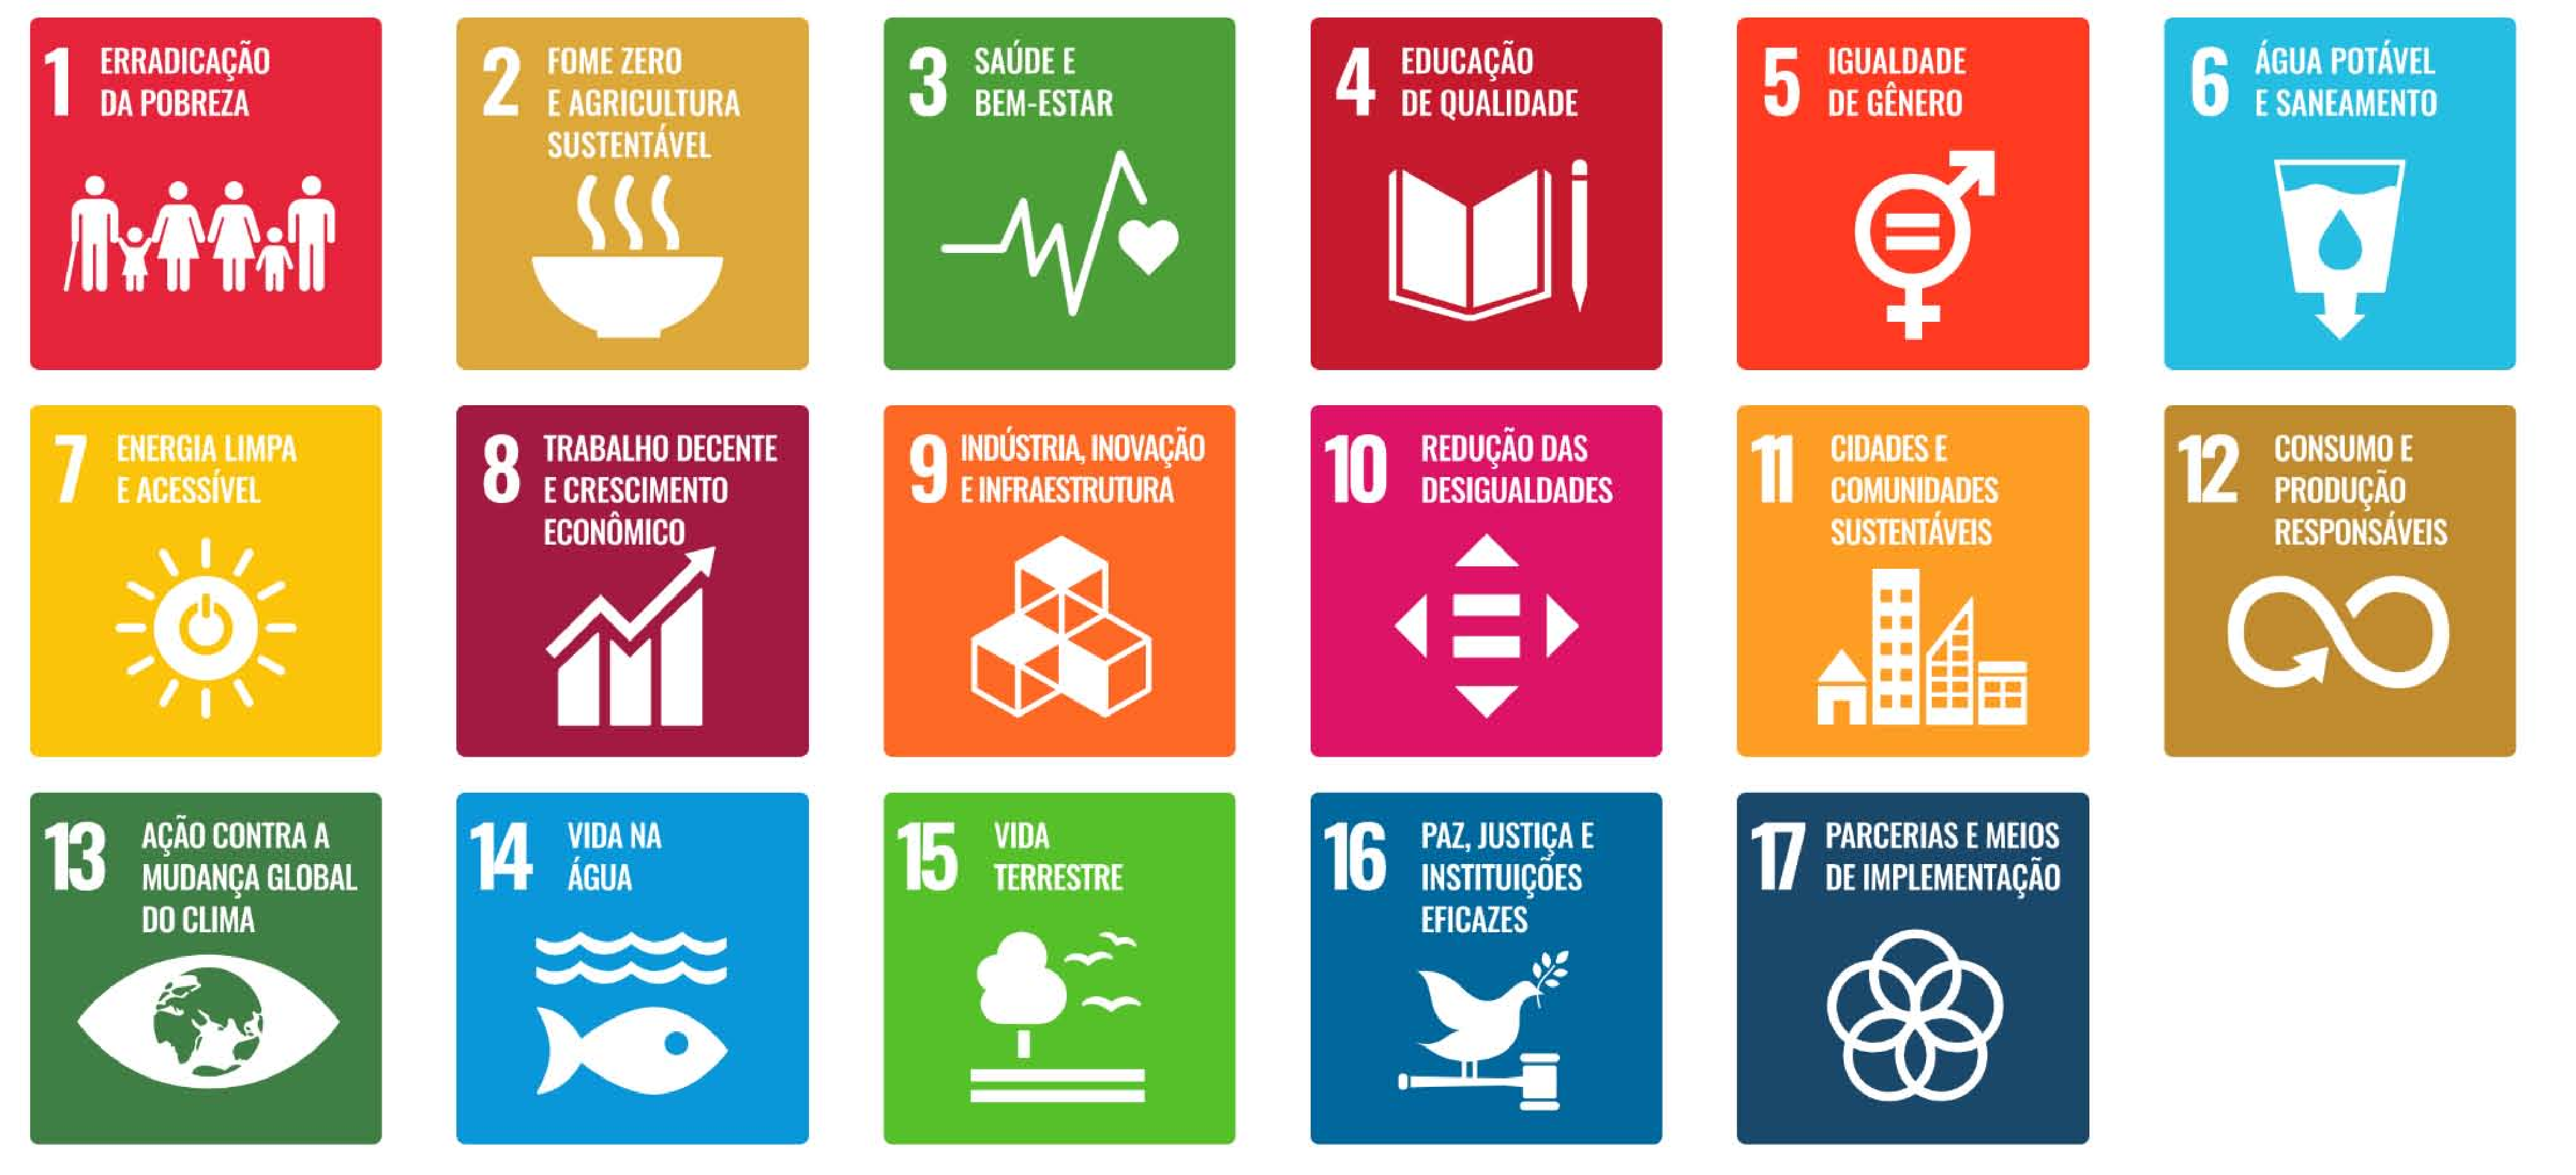
\includegraphics[width=\textwidth]{enc/imagens/ODS-ONU.pdf}
    %Fonte:~\textcite{ARM2013}
\end{figure}



\bigskip

\textbf{Plano de Ensino de uma Disciplina Extensionista (ACE Tipo I)}


\bigskip

Para ser considerada uma ACE a disciplina deve relacionar as competências, estabelecidas pelo NDE do curso de Engenharia
de Computação para um atividade extensionista, de acordo com a Resolução CoEx/CoG. 

A disciplina candidata a ser considerada uma ACE deve apresentar ao menos uma das seguintes características: 

\begin{itemize}[series=listWWNumi,label=\textstyleListLabeli{${\bullet}$}]
\item Projeto e/ou implementação real (hardware e/ou software);
\item Disponibilização em repositório de software público;
\item Interação direta com público externo ao curso;
\item Interação indireta com o público externo ao curso;
\item Disponibilização de software para teste público;
%\item …
\end{itemize}
\bigskip

As atividades propostas nas disciplinas deverão explorar, além dos conhecimentos e habilidades, as competências de uma
ACE. Tais competências devem ser implementadas e avaliadas de acordo com o estabelecido no plano de ensino da
disciplina.


\bigskip

Na disciplina extensionista, ACE Tipo I, há a obrigatoriedade do conteúdo produzido ser externado à comunidade, o que
pode ser realizado na forma de workshops, palestras, apresentação de pôsteres e/ou com as tecnologias de comunicação
existentes, como Redes Sociais (%
%será que vale a pena mencioar? Podem deixar de ser populares e/ou surgirem outras. (TikTok vale?:{}-)
%Helio Crestana Guardia
%2024 Feb 2 13:41
whatsapp, instagram, facebook, linkedin, etc), Fóruns de discussão, vídeos publicados na WEB de caráter “público”,
Webconferência on line, salas virtuais (ex.: google classroom), repositórios públicos de software, etc. garantindo
assim a interação com o público externo (comunidade interna e externa à UFSCar).


\bigskip

O conteúdo da disciplina extensionista (ACE do tipo I) a ser externado ao público interno e externo à UFSCar pode ser
parcial, durante a execução da disciplina, ou total, incluindo a apresentação de projetos, que podem ser divulgados
prévia e amplamente nos meios de comunicação digital%
%Pensar se vale a pena listar ou deixar aberto.
%Helio Crestana Guardia
%2024 Feb 2 13:45
, inclusive nos oficiais, em pelo menos um deles, como o “site” do Departamento de Computação - DC da UFSCar, \ Boletim
informativo da UFSCar, Boletim de oportunidades da UFSCar, etc.

%\end{document}
%\includepdf[pages=-]{anexos/extensao.pdf}

\chapter{Regulamento de Atividades Complementares}~\label{cha:atividades_complementares}
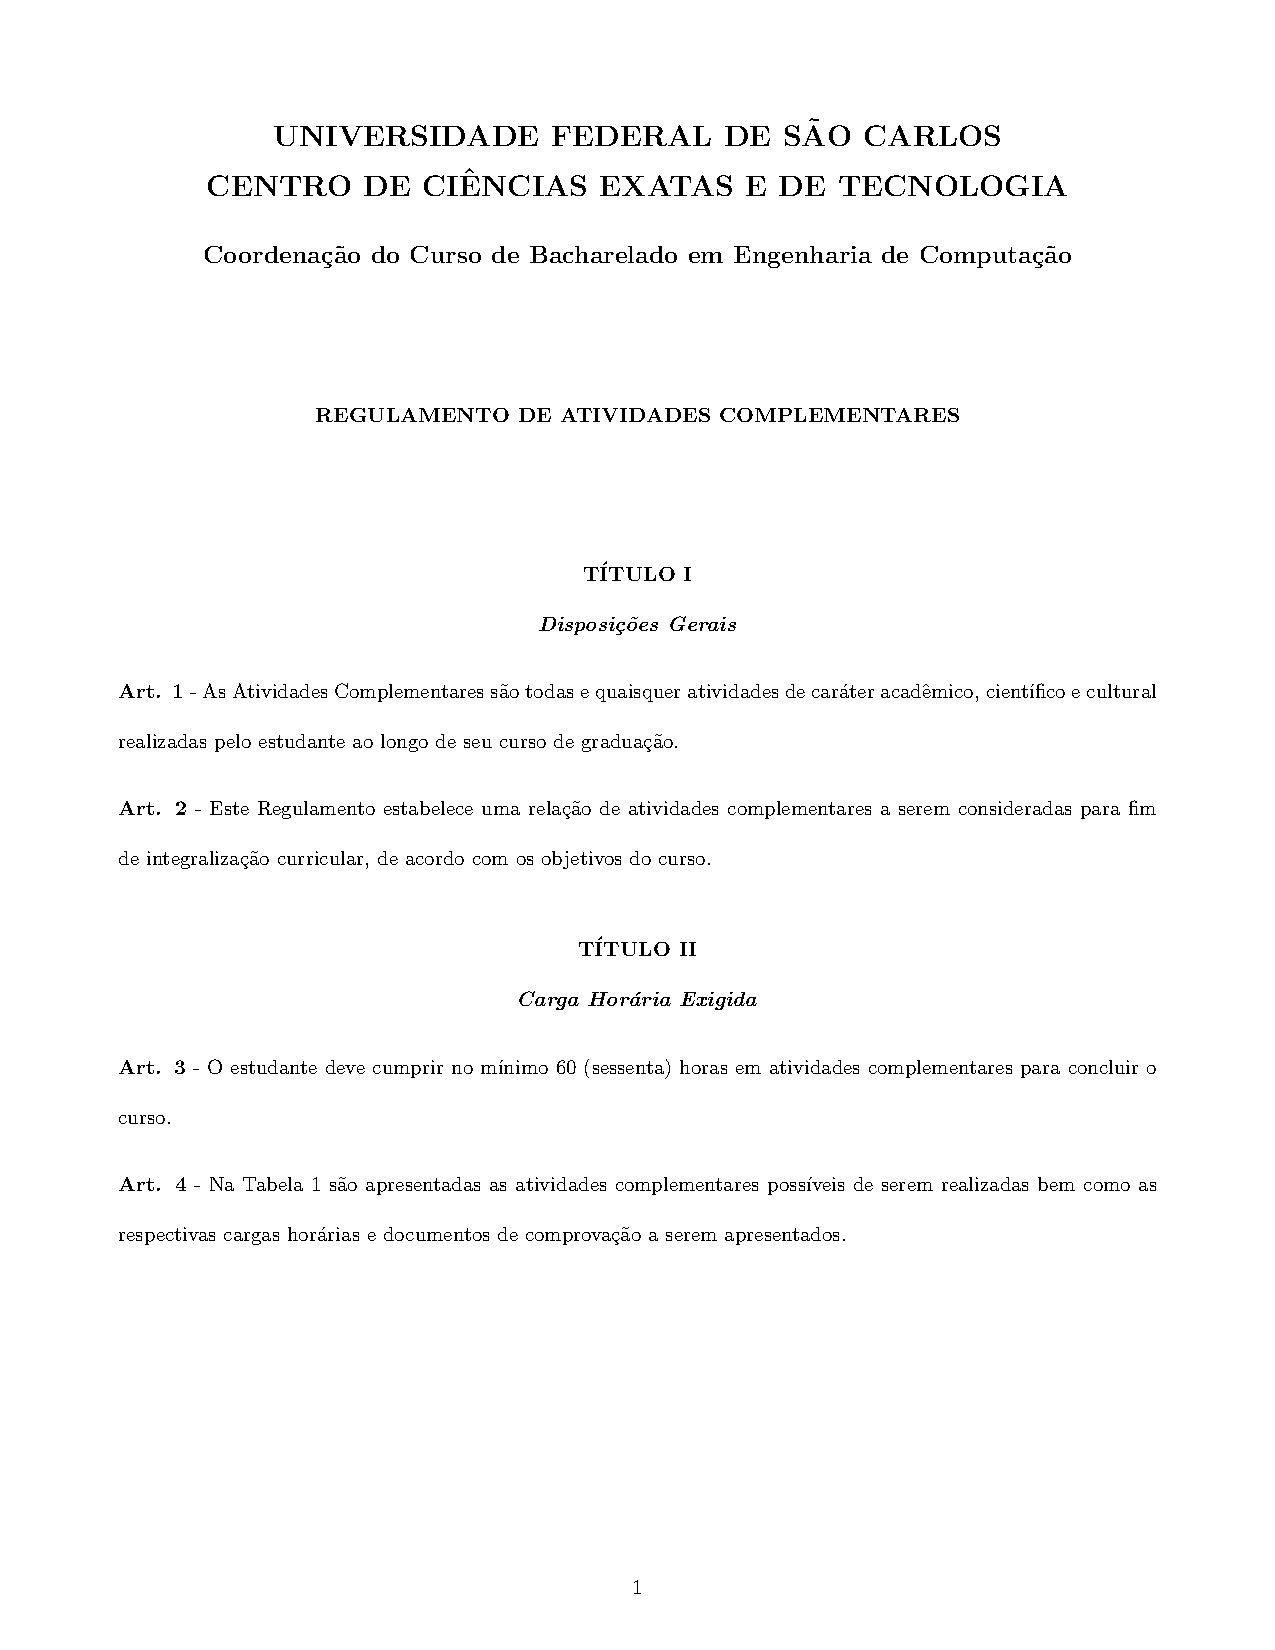
\includepdf[pages=-]{anexos/ativcompl.pdf}

\chapter{Regulamento do Estágio Curricular Obrigatório e Não-obrigatório}~\label{cha:estagio}
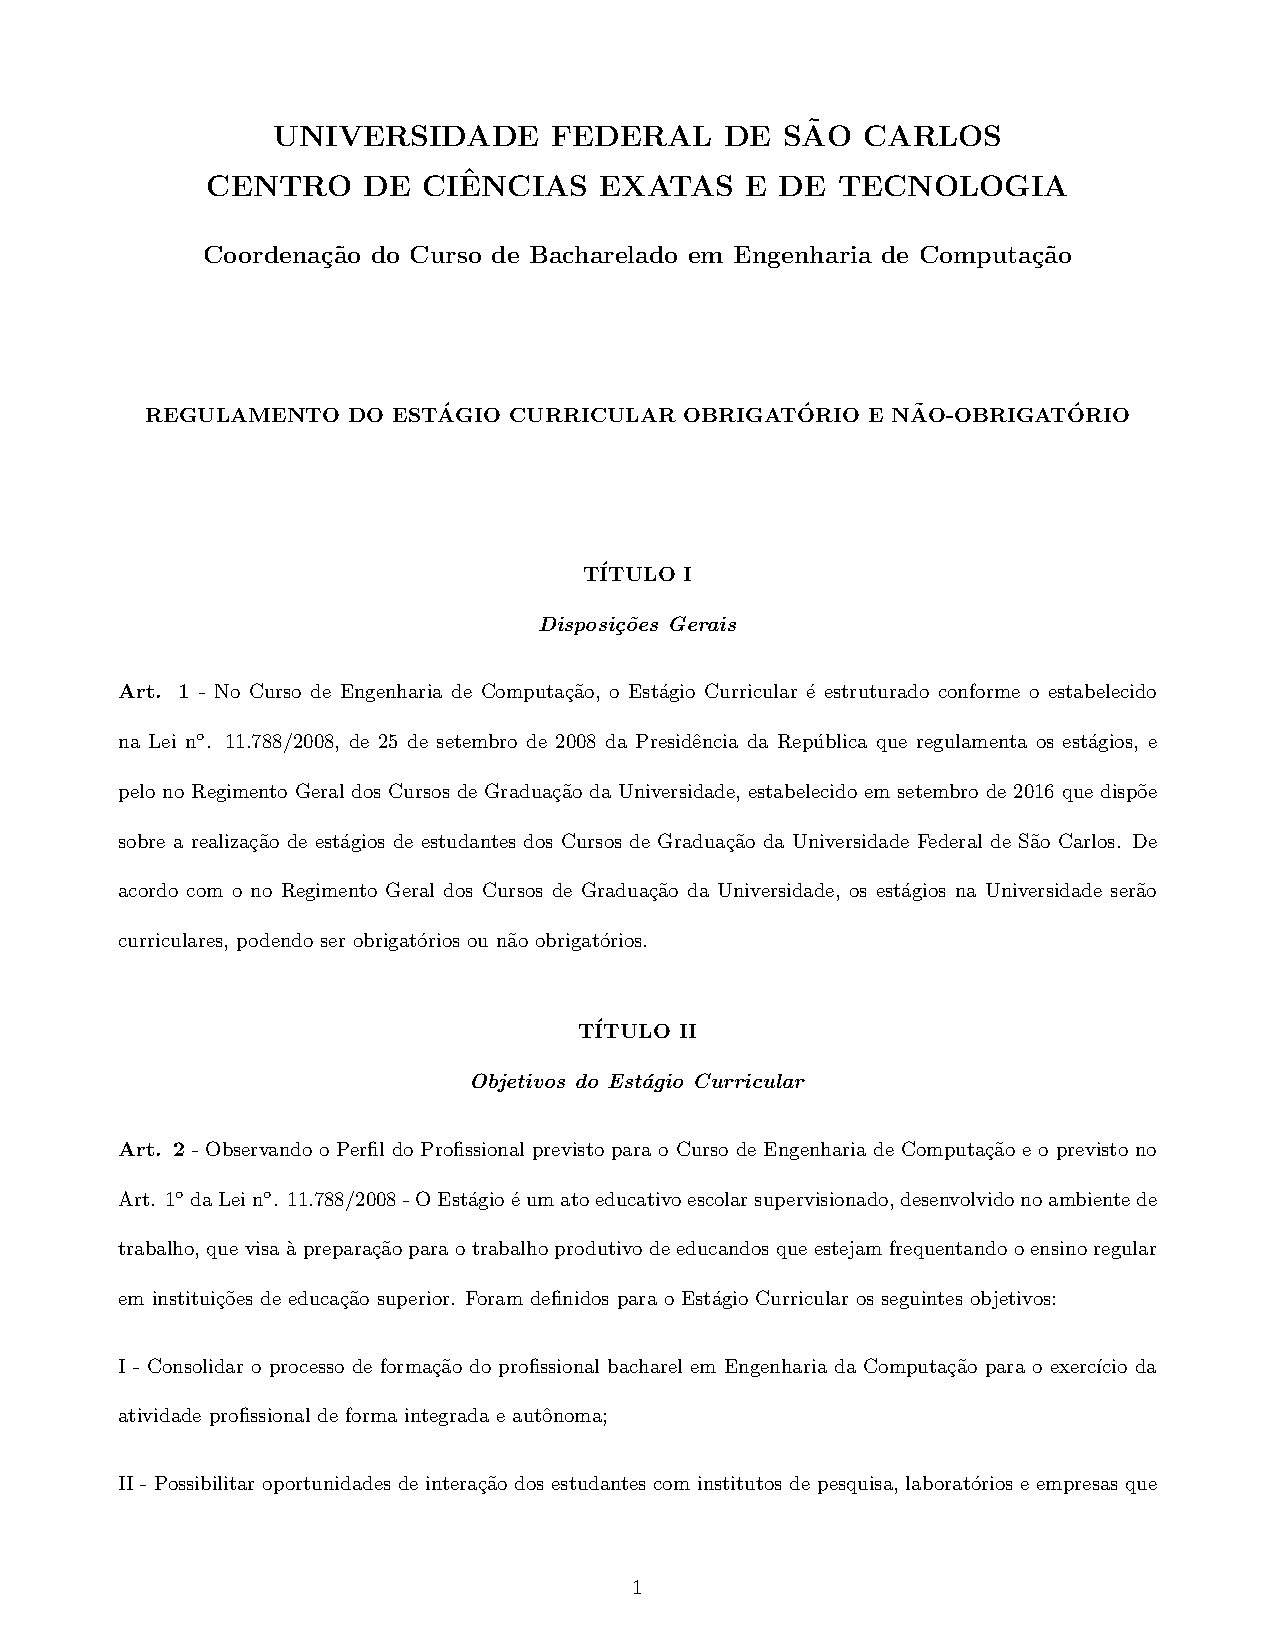
\includepdf[pages=-]{anexos/estagio.pdf}

\chapter{Regulamento do Trabalho de Conclusão de Curso}~\label{cha:tcc}
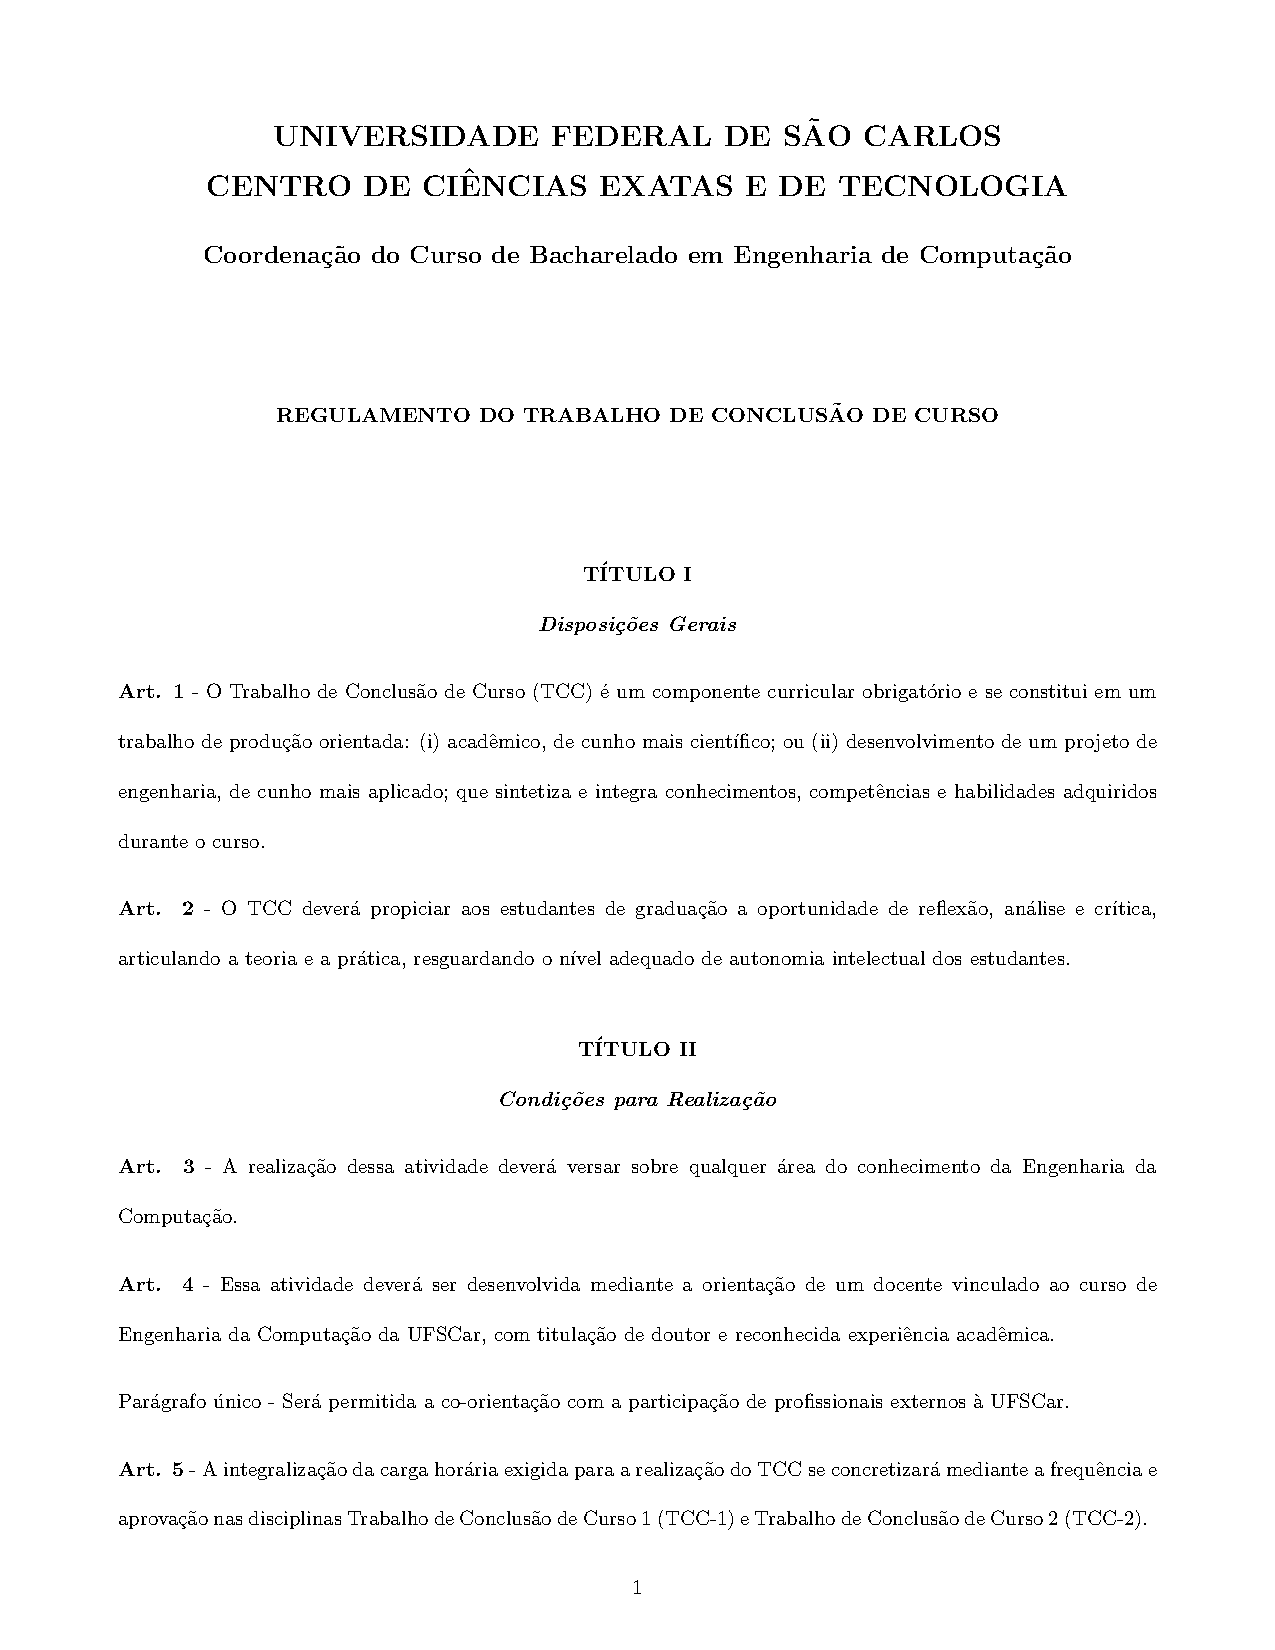
\includepdf[pages=-]{anexos/tcc.pdf}


%%%%%%%%%%%  Informações para gerenciamento

{
    \section*{Disciplinas que ainda não possuem competências especificadas}
    
    Relação de disciplinas que não tiveram as competências preenchidas:
        \color{red}
    \begin{itemize}
        \ExecuteLista{\Discipl}{%
            aed1,aed2,
            algelin,
            am1,am2,
            arq1,arq2,arqad,
            asp,bd,bdcd,calnum,calculo1,calculo2,calculo3,
            cap,
            cg,
            circeletricos,circeletronicos1,
            circeletronicos2,compiladores,controle,controle1,
            controle2,devops,dm,dw1,dw2,empreend,engsis,es1,
            es2,estagio,estagio,fisexpa,fisexpb,fisica1,
            fisica3,ga,ia,ihc,ipa,ld,libras,lm,md,metcient,
            musical,om,ori,paa,pde,pdi,pdi3dv,pibd,plp,
            pmac,poo,pooa,ppd,probest,projsisemb,protsisdigan,
            psd,pvd,rc,robosautonomos,robotica,sc,sd,sem1,sem2,
            sereqdif,siai,sistdin,sistdist,so,tc,tcc1,tcc2,teccom,
            vc
        }{%
            \SeExisteAtributo{\Discipl}{competencias}{}{\item \Atributo{\Discipl}{nome}}
        }
    \end{itemize}
}

{
    \section*{Atualização das competências das disciplinas}
    
    Relação de disciplinas com última dada de \textbf{revisão}:
    \begin{itemize}
        \ExecuteLista{\Discipl}{%
            aed1,aed2,
            algelin,
            am1,am2,
            arq1,arq2,arqad,
            asp,bd,bdcd,calnum,calculo1,calculo2,calculo3,
            cap,
            cg,
            circeletricos,circeletronicos1,
            circeletronicos2,compiladores,controle,controle1,
            controle2,devops,dm,dw1,dw2,empreend,engsis,es1,
            es2,estagio,fisexpa,fisexpb,fisica1,
            fisica3,ga,ia,ihc,ipa,ld,libras,lm,md,metcient,
            musical,om,ori,paa,pde,pdi,pdi3dv,pibd,plp,
            pmac,poo,pooa,ppd,probest,projsisemb,protsisdigan,
            psd,pvd,rc,robosautonomos,robotica,sc,sd,sem1,sem2,
            sereqdif,siai,sistdin,sistdist,so,tc,tcc1,tcc2,teccom,
            vc
        }{%
            \item \Atributo{\Discipl}{nome} - \Atributo{\Discipl}{codigo} --
            \SeExisteAtributo{\Discipl}{dataatualizacao}{%
                \Atributo{\Discipl}{dataatualizacao}%
            }{%
                \textcolor{red!80!black}{\textbf{Sem data de revisão!}}
            }
        }
    \end{itemize}
}



%%%%%%%%%%%%%%%%%%%% Projetos pedagógicos Anteriores %%%%%%%%%%%%%%%%%%%%

% \chapter{Projeto Pedagógico 2006}~\label{cha:ppc2006}
% 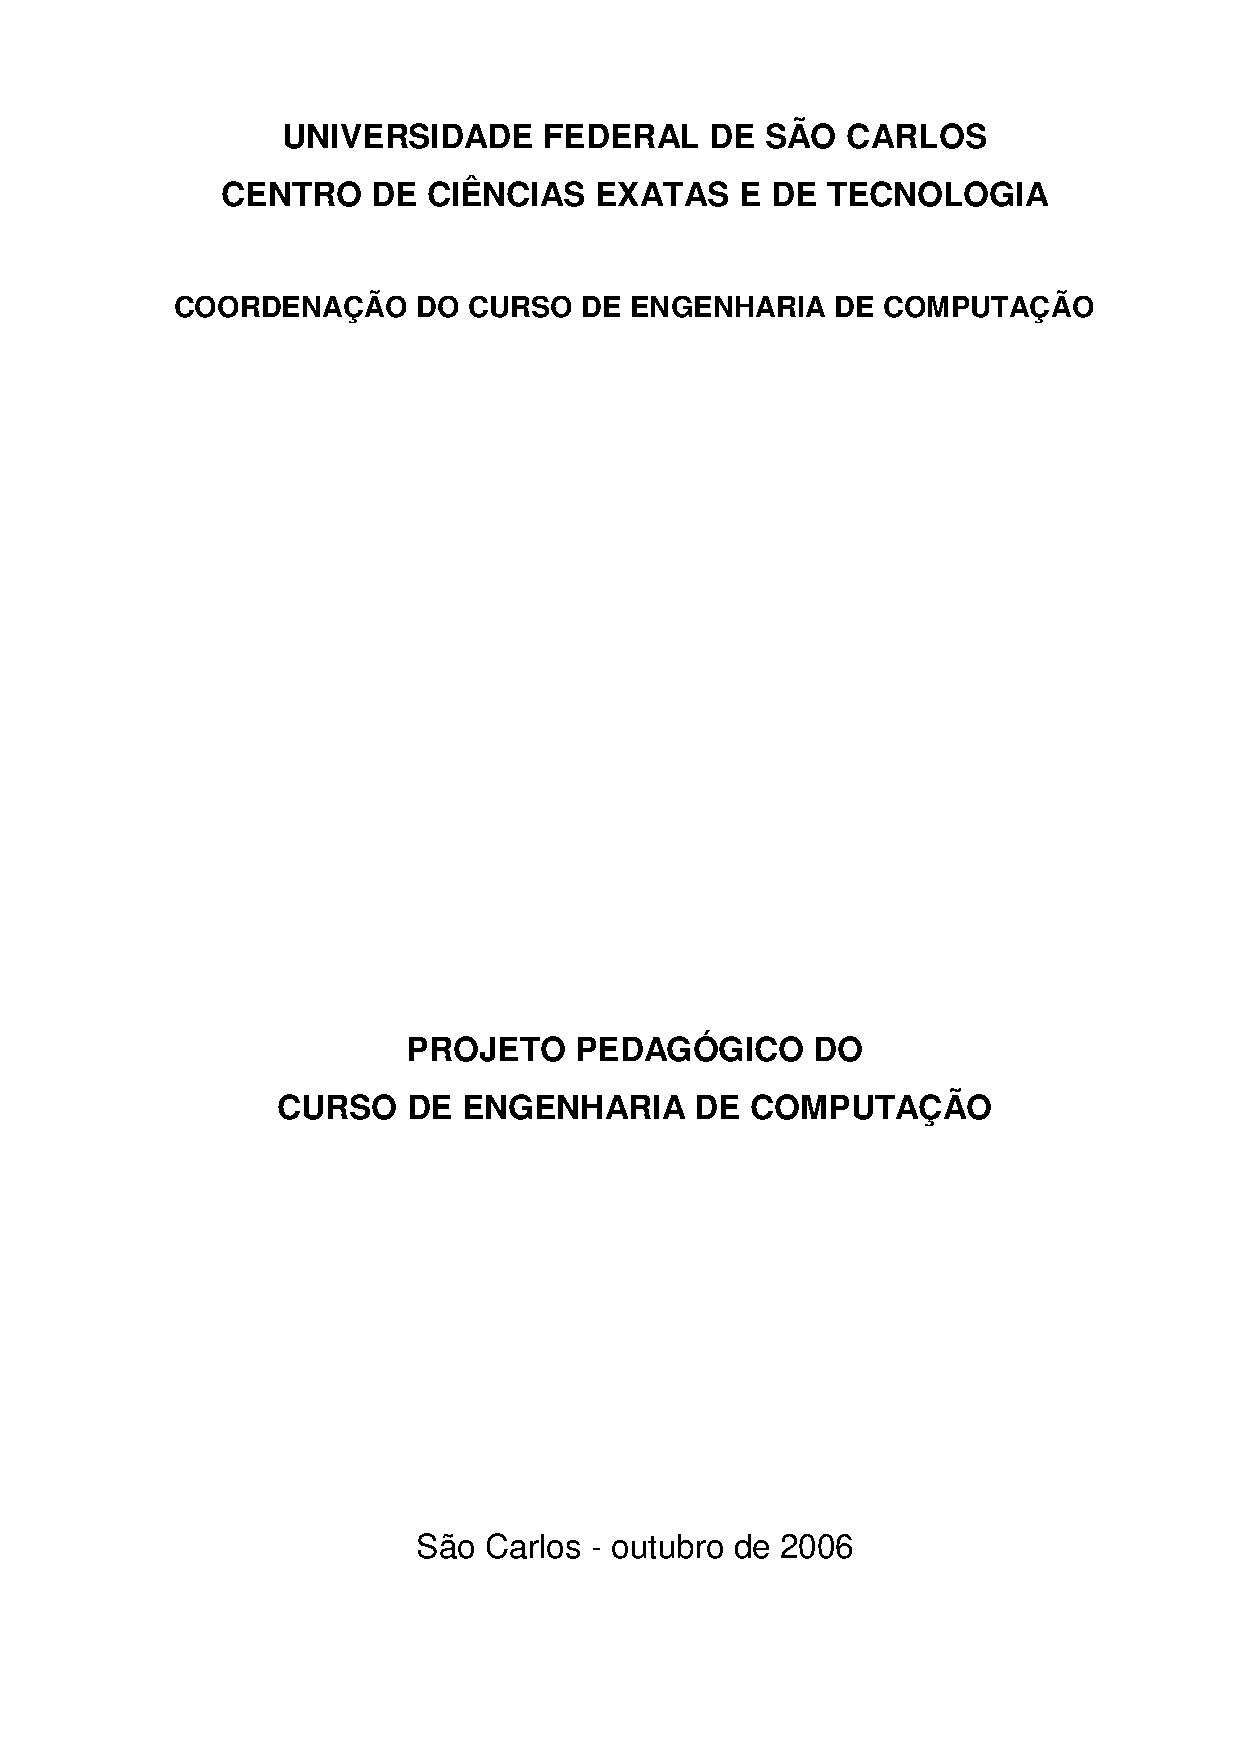
\includepdf[pages=-]{anexos/pp2006.pdf}

% \chapter{Matriz Curricular de 1999}~\label{cha:Matriz1999}
% 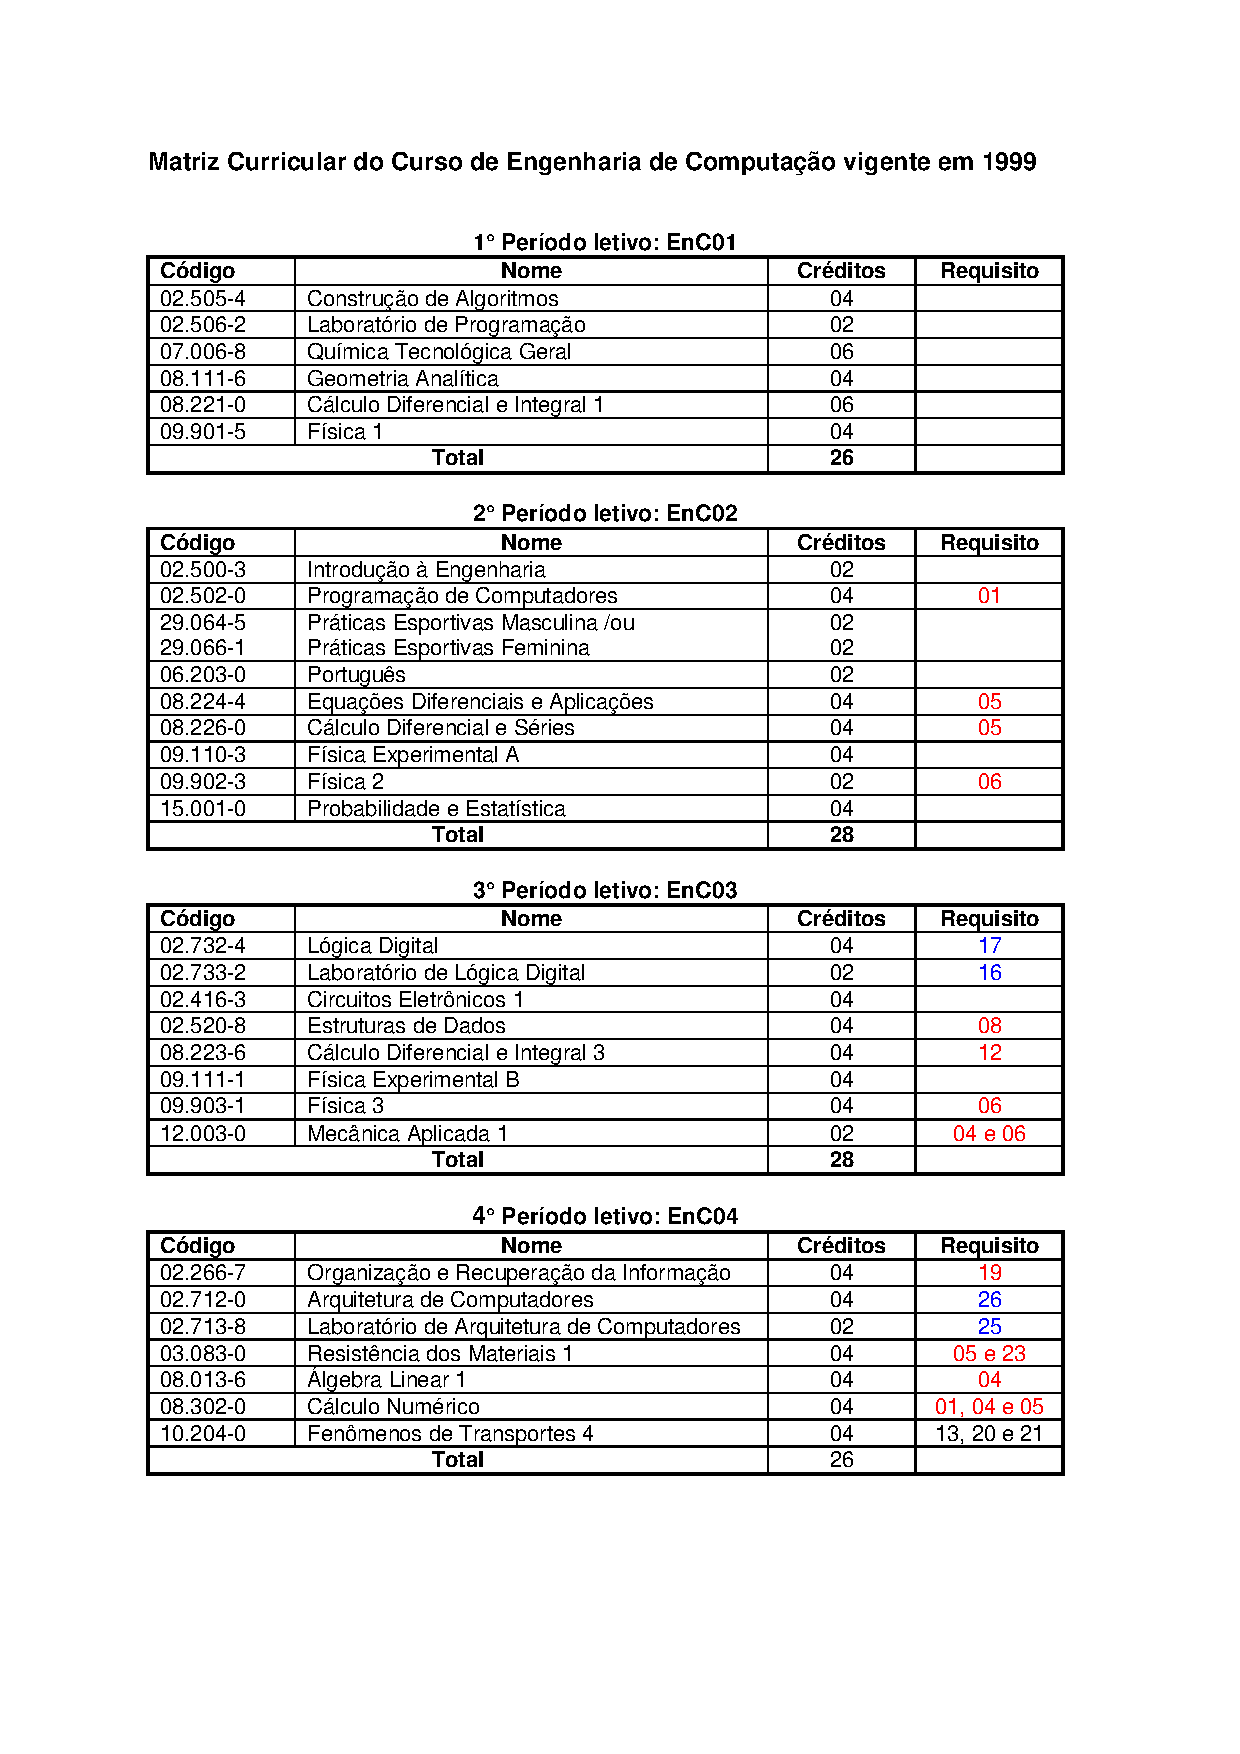
\includepdf[pages=-]{anexos/Matriz1999.pdf}

% \chapter{Matriz Curricular de 1992}~\label{cha:Matriz1992}
% 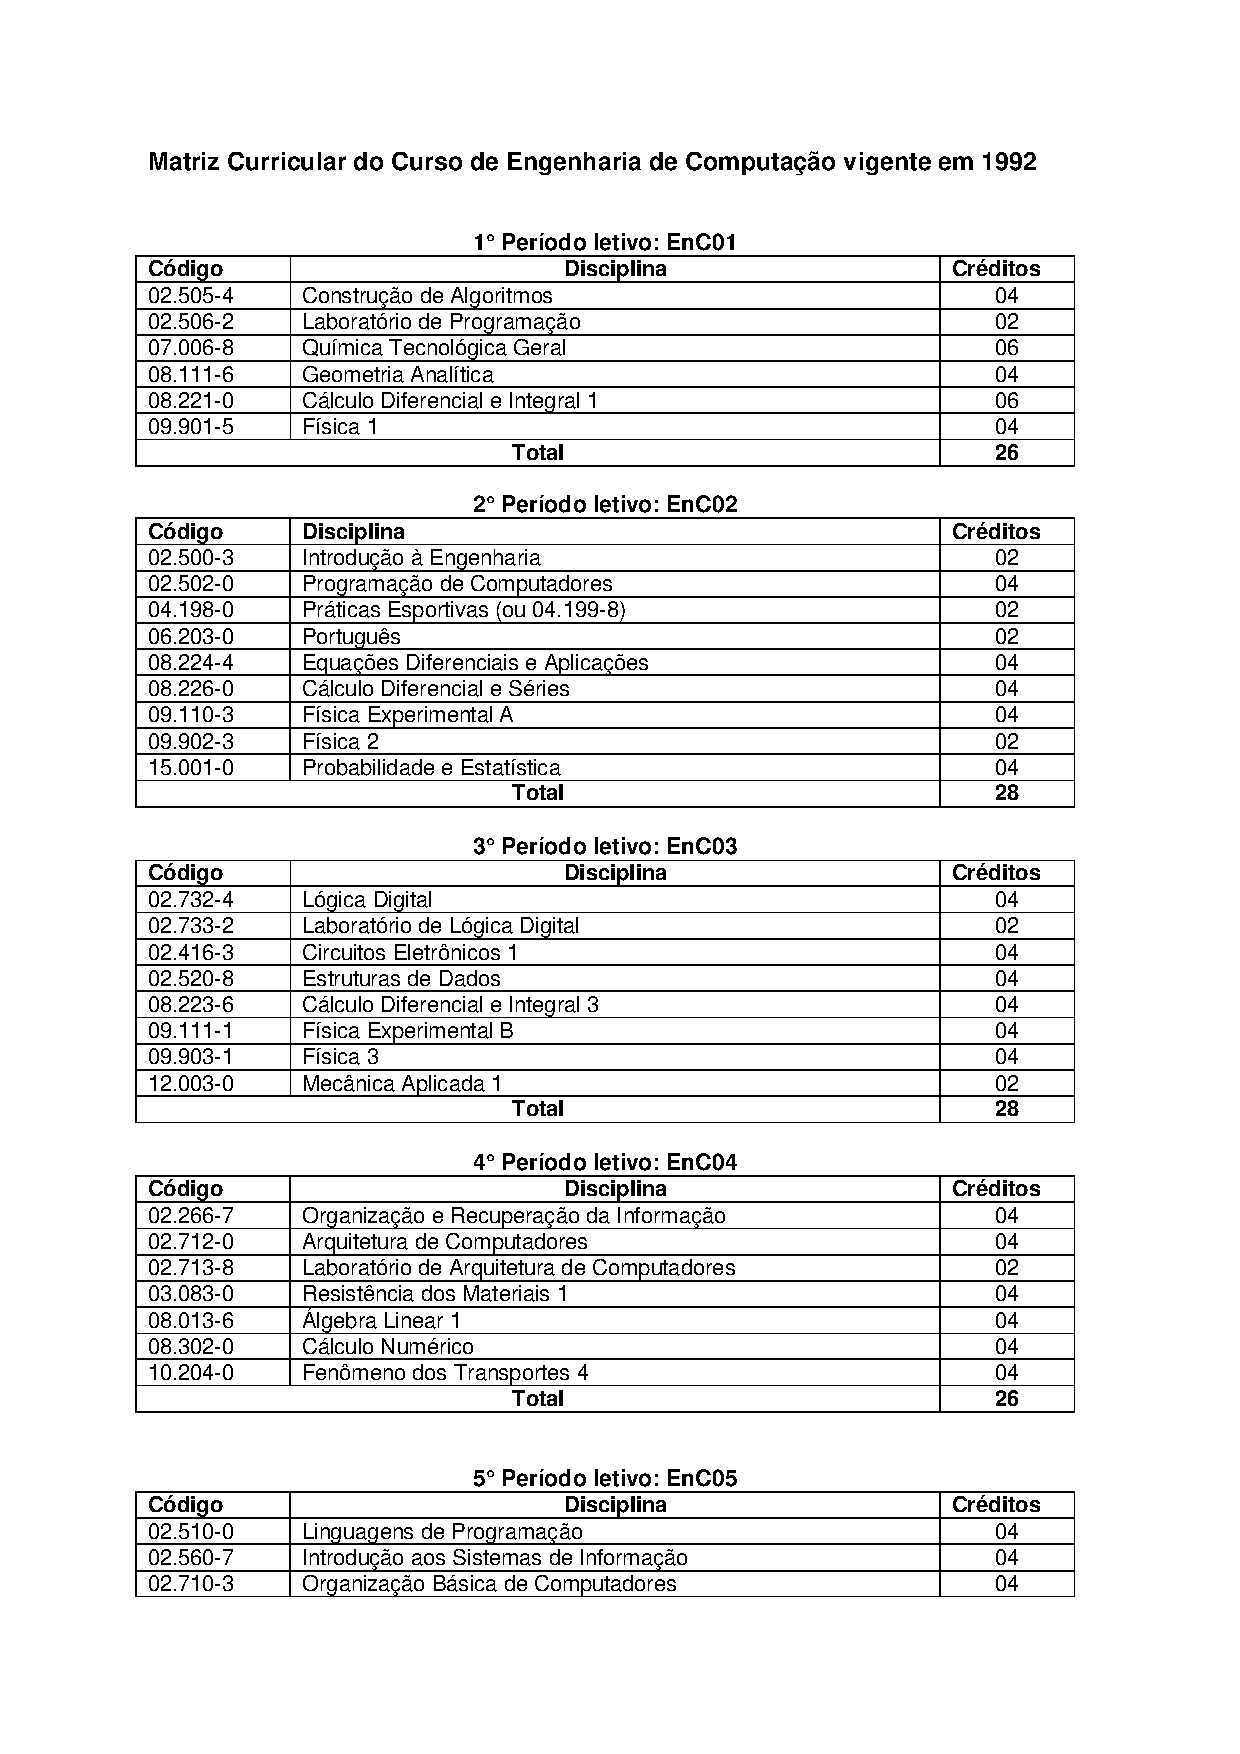
\includepdf[pages=-]{anexos/Matriz1992.pdf}


%%%%%%%%%%%%%%%%%%%% Avaliacoes %%%%%%%%%%%%%%%%%%%%

% \chapter{Avaliação Externa MEC}~\label{cha:AvaliacaoMEC}
% 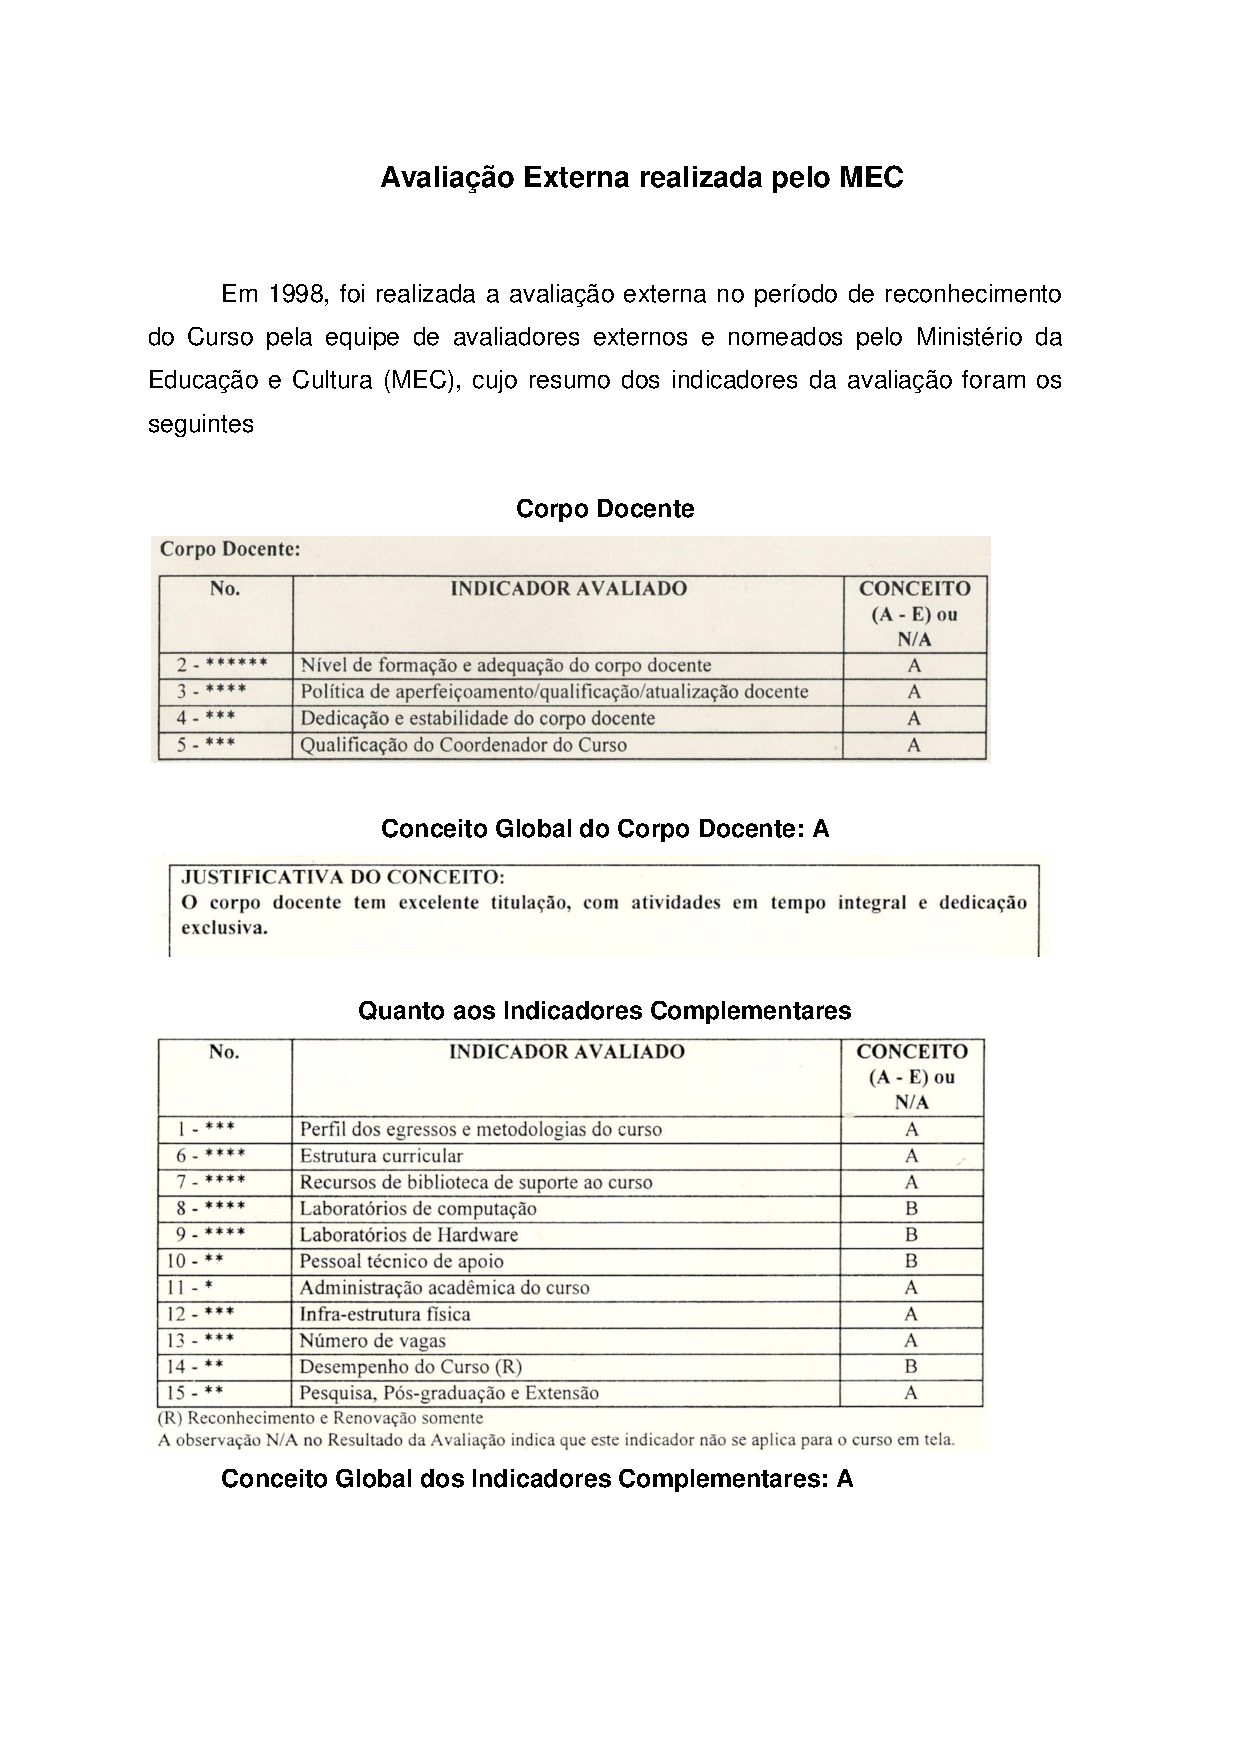
\includepdf[pages=-]{anexos/Avaliacao_externaMEC.pdf}

% \chapter{Programa de Avaliação Institucional das Universidades Brasileiras (PAIUB)}~\label{cha:PAIUB}
% 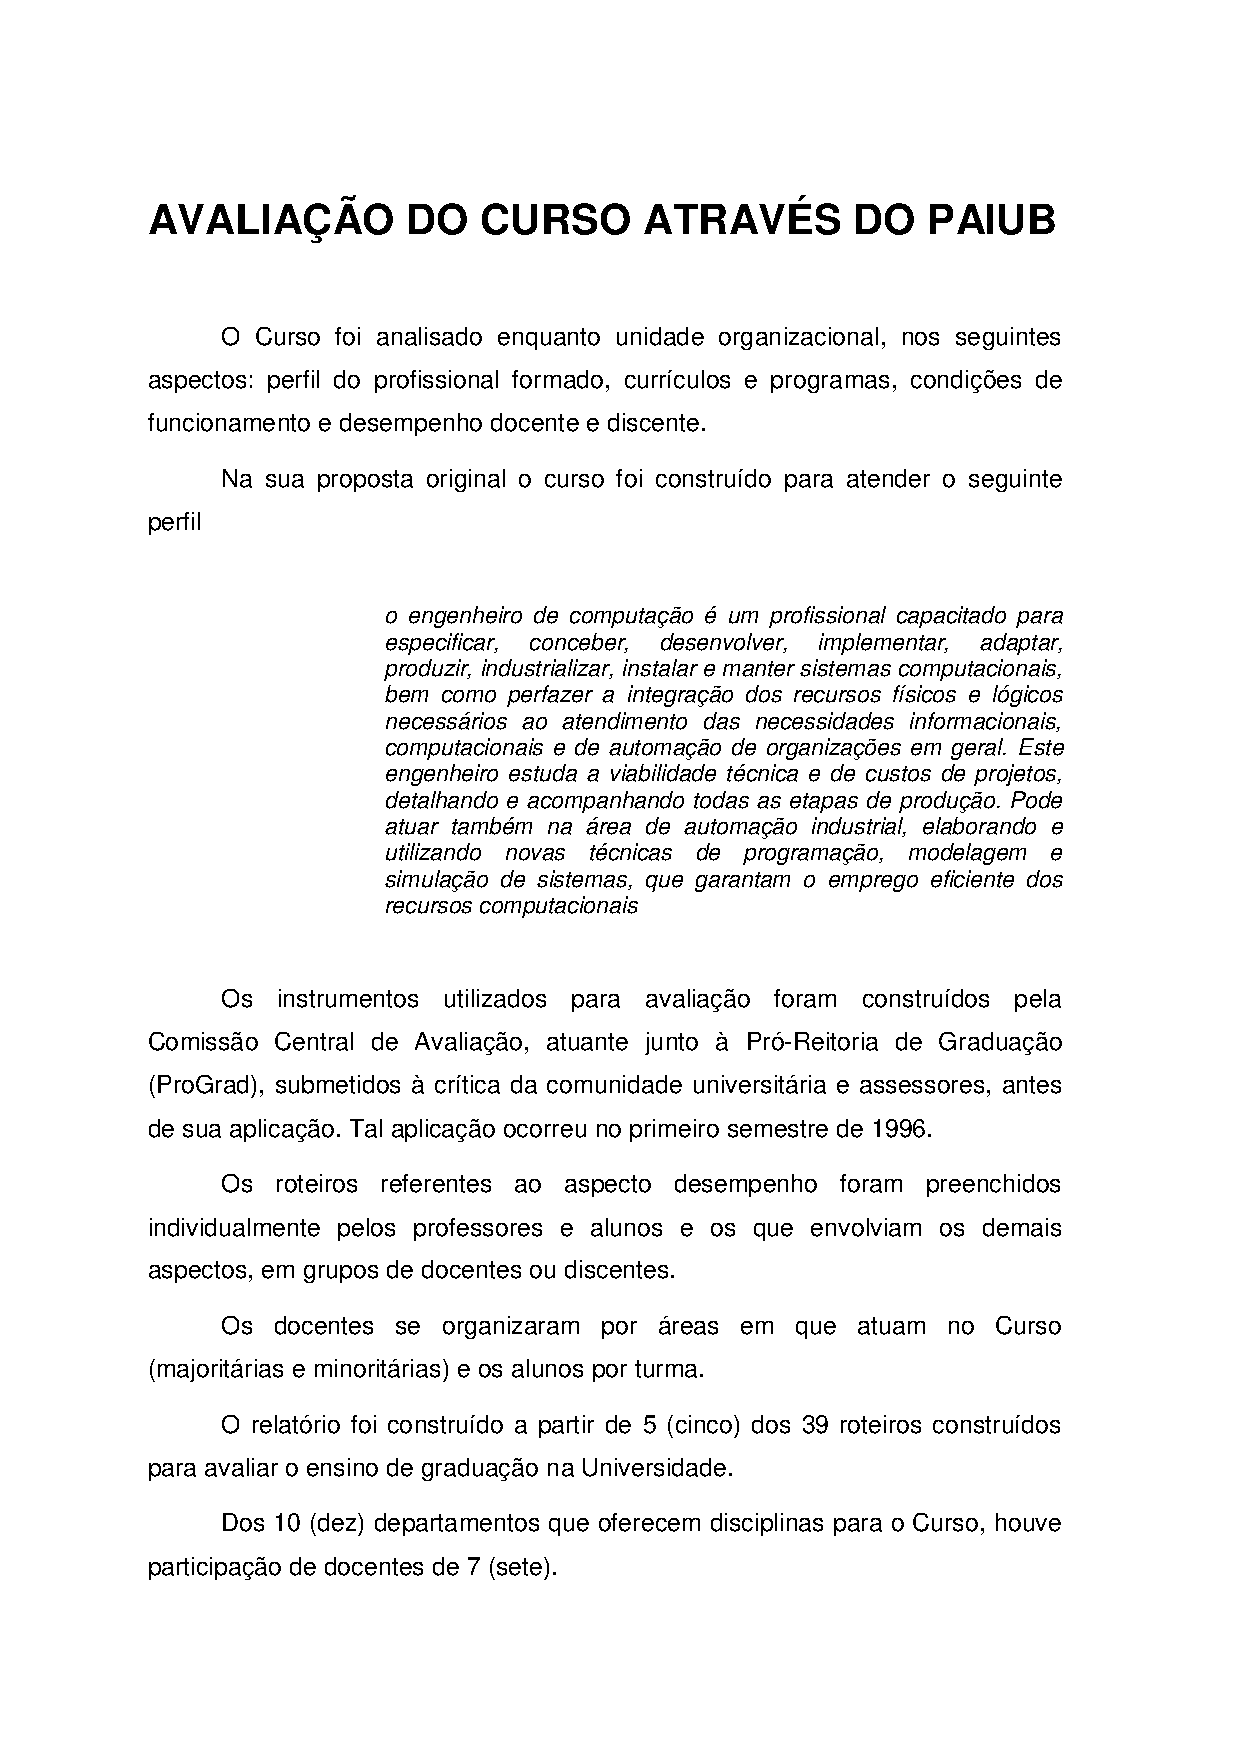
\includepdf[pages=-]{anexos/PAIUB.pdf}

% \chapter{Avaliação UFSCar/CPA}~\label{cha:CPA}
% 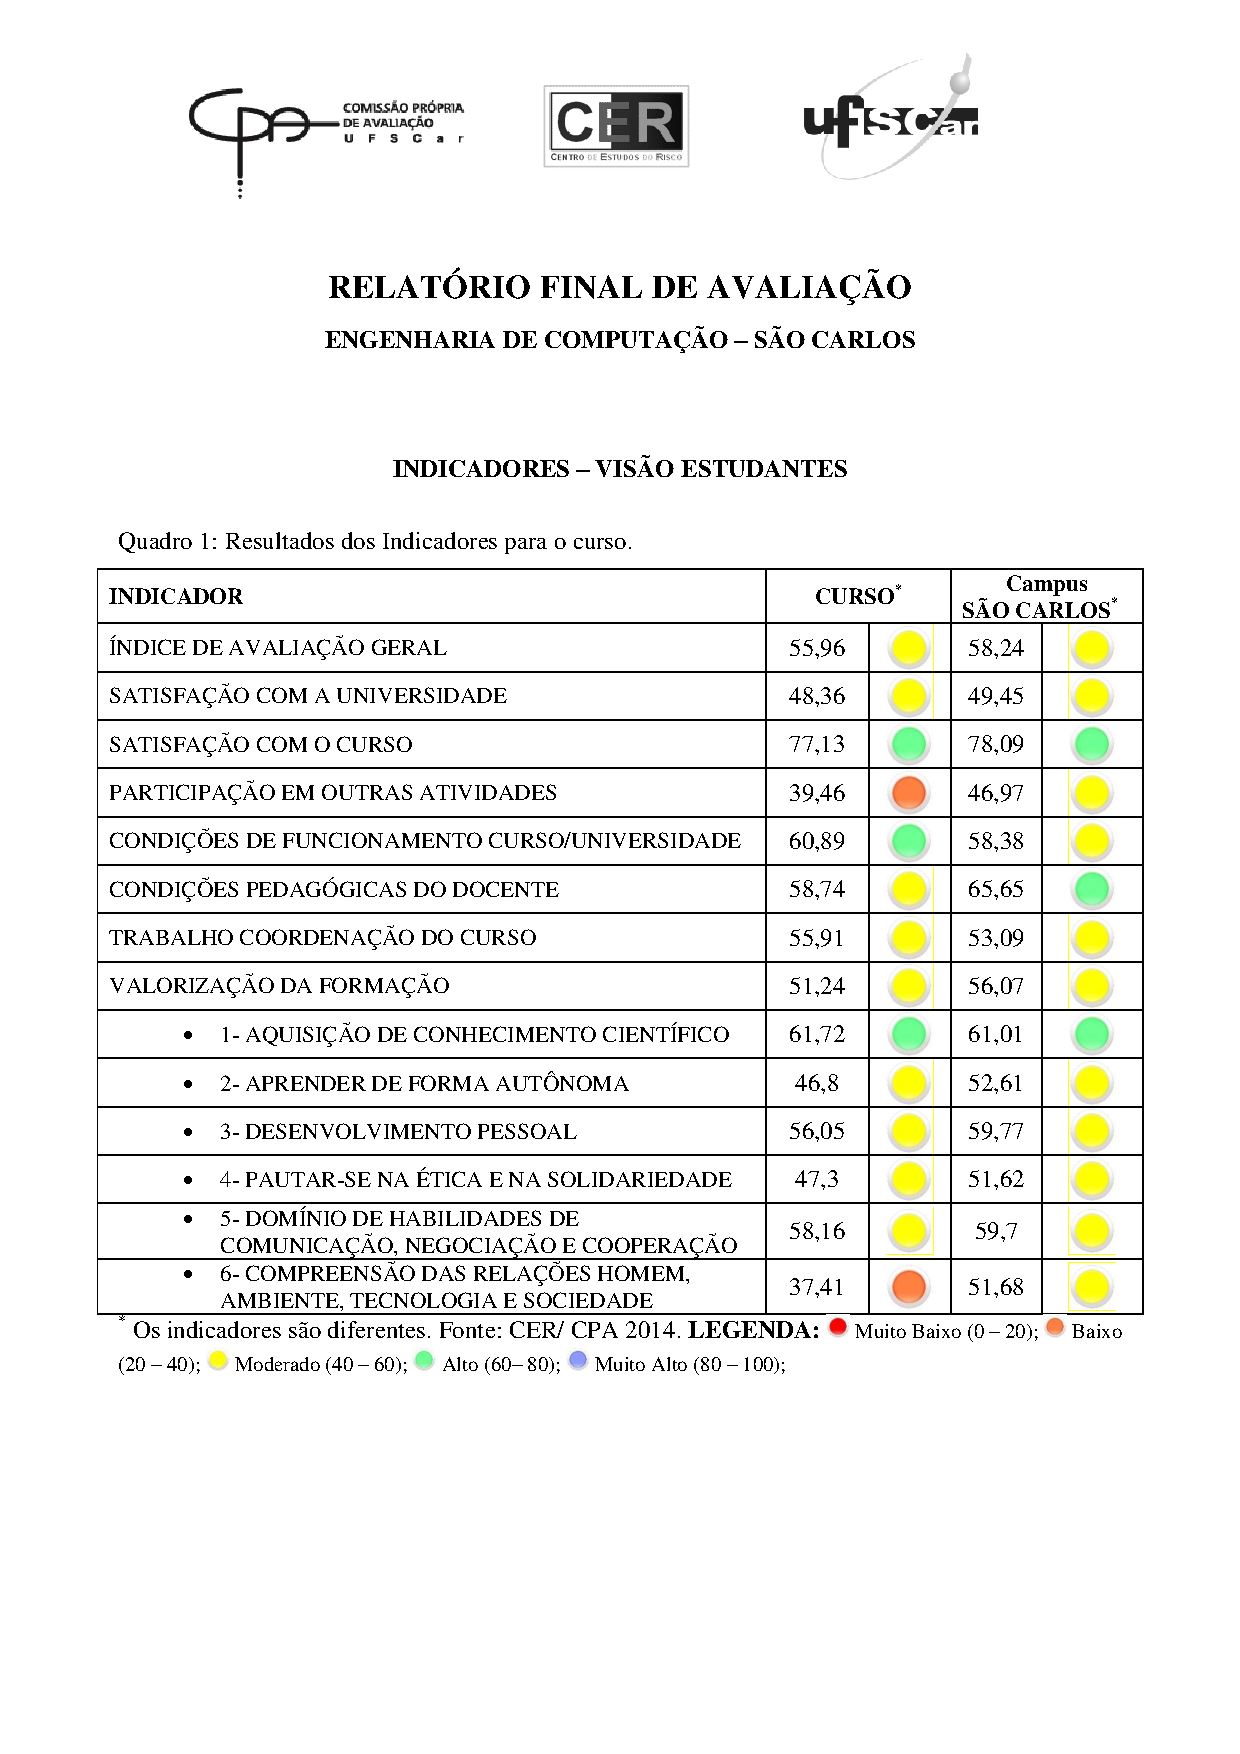
\includepdf[pages=-]{anexos/UFSCar_CPA.pdf}


\end{document}